\documentclass[12pt,a4paper]{article}
\usepackage[utf8]{inputenc}
\usepackage[T1]{fontenc}
\usepackage{graphicx}
\usepackage{geometry}
\usepackage{setspace}
\usepackage{array}
\usepackage{xcolor}
\usepackage{changepage}
\usepackage{caption}
\usepackage{tikz}
\usepackage[T5]{fontenc} % For Vietnamese
\usepackage[hidelinks]{hyperref} % Enables hyperlinks
\usepackage{titlesec}
\usepackage{enumitem}
\usepackage{graphicx}
\usepackage{float}
\usepackage{array} % for better column control
\usepackage{makecell} % for better cell formatting
\usepackage{longtable}
\usepackage{etoolbox}
% HEADER AND FOOTER STUFF
\usepackage{fancyhdr}
\usepackage{lastpage}
\usepackage{enumitem} % in preamble
\usepackage{subcaption}

% Set globally for all figures
\captionsetup{skip=6pt} % Default is usually 10pt

\pagestyle{fancy}
\fancyhead{}
\fancyfoot{}
% \fancyfoot[R]{\thepage}
\fancyfoot[C]{\makebox[\textwidth][r]{Page \thepage\ of \pageref{LastPage}}}
\renewcommand{\headrulewidth}{0pt}

% Define colors first before using them
\definecolor{sectioncolor}{RGB}{0, 0, 0} % Using black for section headers
\definecolor{usthblue}{RGB}{36, 64, 142}
\definecolor{usthred}{RGB}{237, 50, 36}

% Define horizontal lines
\newcommand{\horrule}[1]{\rule{\linewidth}{#1}}

% Change section numbering to Roman numerals
\renewcommand\thesection{\Roman{section}}
\renewcommand\thesubsection{\arabic{section}.\arabic{subsection}}

% Adjust section formatting with rule line underneath
\titleformat{\section}
  {\normalfont\Large\bfseries\color{sectioncolor}}
  {\thesection}{1em}{}[{\titlerule[0.8pt]}]
\titleformat{\subsection}
  {\normalfont\large\bfseries\color{sectioncolor}}
  {\thesubsection}{1em}{}

\usetikzlibrary{calc}

% Set page margins
\geometry{left=3.5cm, right=2.0cm, top=2.5cm, bottom=2.5cm}

\begin{document}

\begin{titlepage}
    \begin{center}
        % Create a frame around the entire page
        \begin{tikzpicture}[remember picture, overlay]
            \draw [line width=1pt]
                ([xshift=3.5cm, yshift=-2.5cm]current page.north west) rectangle
                ([xshift=-2.0cm, yshift=2.5cm]current page.south east);
        \end{tikzpicture}
    
        {\normalsize \textbf{UNIVERSITY OF SCIENCE AND TECHNOLOGY OF HANOI}} \\
        {\normalsize {Department of Information and Communication Technology}} \\
        
        \vspace{1cm}
        
\includegraphics[width=5cm]{images/logo_USTH.png}
        
        \vspace{2cm}
        {\Huge {\textbf{Report Labwork 1}}} \\
        \vspace{0.5cm}
        {\LARGE \textbf{Gradient Descent}} \\

        \vspace{1.5cm}
        By\\
        Ngo Quang Truong\\
        2540106\\
        
        \vfill
        {\large \textbf{Hanoi, May 2026}}
    \end{center}
\end{titlepage}

% TABLE OF CONTENT
\renewcommand{\contentsname}{TABLE OF CONTENTS} % Change "Contents" to "My Custom Title"
\clearpage
\pagestyle{empty}
\newpage
\thispagestyle{empty}
\tableofcontents
\clearpage

% When starting the main content:
\newpage
\clearpage
\pagenumbering{arabic}  % Switch back to arabic numbers
\setcounter{page}{1}    % Reset page counter again for main content
\pagestyle{fancy}  
\pagenumbering{arabic}  % Switch back to arabic numbers
\setcounter{page}{1}    % Reset page counter again for main content

% I. INTRODUCTION
\newpage
\setcounter{page}{1}  % Reset page numbering so the introduction starts from page 1
\section{INTRODUCTION}\label{sec:intro}
  \indent
  Gradient Descent is an iterative optimization algorithm used to minimize a cost function by adjusting model parameters in the direction of the steepest descent of the function’s gradient. In simple terms, it finds the optimal values of weights and biases by gradually reducing the error between predicted and actual outputs.Given a differentiable function f : R →R and its first-order derivative f, the algorithm repeatedly moves the current estimate of the minimum in the direction that decreases f most steeply—i.e. opposite to the gradient.

% II. SYSTEM ANALYSIS
\newpage
\section{MATHEMATIC BACKGROUND}\label{sec:mathematic_background}
  % 2.1 Problem formulation
  \subsection{Problem formulation}
  \label{sec:problem_formulation}
  \indent 
    
    We seek the minimiser
\[
  x^* \;=\; \arg\min_{x \in \mathbb{R}}\; f(x),
\]
where $f$ is assumed differentiable and the derivative $f'$ is known analytically
(or can be computed).

\subsection{The update rule}

Starting from an initial guess $x_0$, gradient descent produces the sequence
\[
  \boxed{x_{k+1} \;=\; x_k \;-\; r \cdot f'(x_k)}, \qquad k = 0, 1, 2, \ldots
\]
where $r > 0$ is the \textbf{learning rate} (also called step size).

\paragraph{Intuition.}
The derivative $f'(x_k)$ points uphill; subtracting a fraction of it moves
$x$ downhill.  If $r$ is too small the progress is slow; if $r$ is too large
the iterates may overshoot and oscillate or diverge.

\subsection{Convergence criterion}

We stop when the gradient magnitude drops below a tolerance $\varepsilon$:
\[
  |f'(x_k)| \;<\; \varepsilon \;\approx\; 10^{-8}.
\]

\subsection{Test function}

Throughout this report we use:
\[
  f(x) = x^2, \qquad f'(x) = 2x.
\]
The unique global minimum is $x^* = 0$ with $f(x^*) = 0$.

  % 2.2 System Requirements
  % \subsection{System Requirements}
  % \indent

This section presents an \textbf{overview of the entire system requirements} through a high-level use case diagram. It also includes details visualizations of each \textbf{key module and feature under my responsibility}.


\subsubsection{System Requirements Overview}
\noindent
\begin{minipage}{\textwidth}
    \setlength{\parindent}{2em}
    From the modules and user roles defined in \textbf{\autoref{sec:scope} \nameref{sec:scope}}, this section presents a visual overview of the entire systems requirements and the associated user roles.
\end{minipage}

\begin{figure}[H]
    \centering
    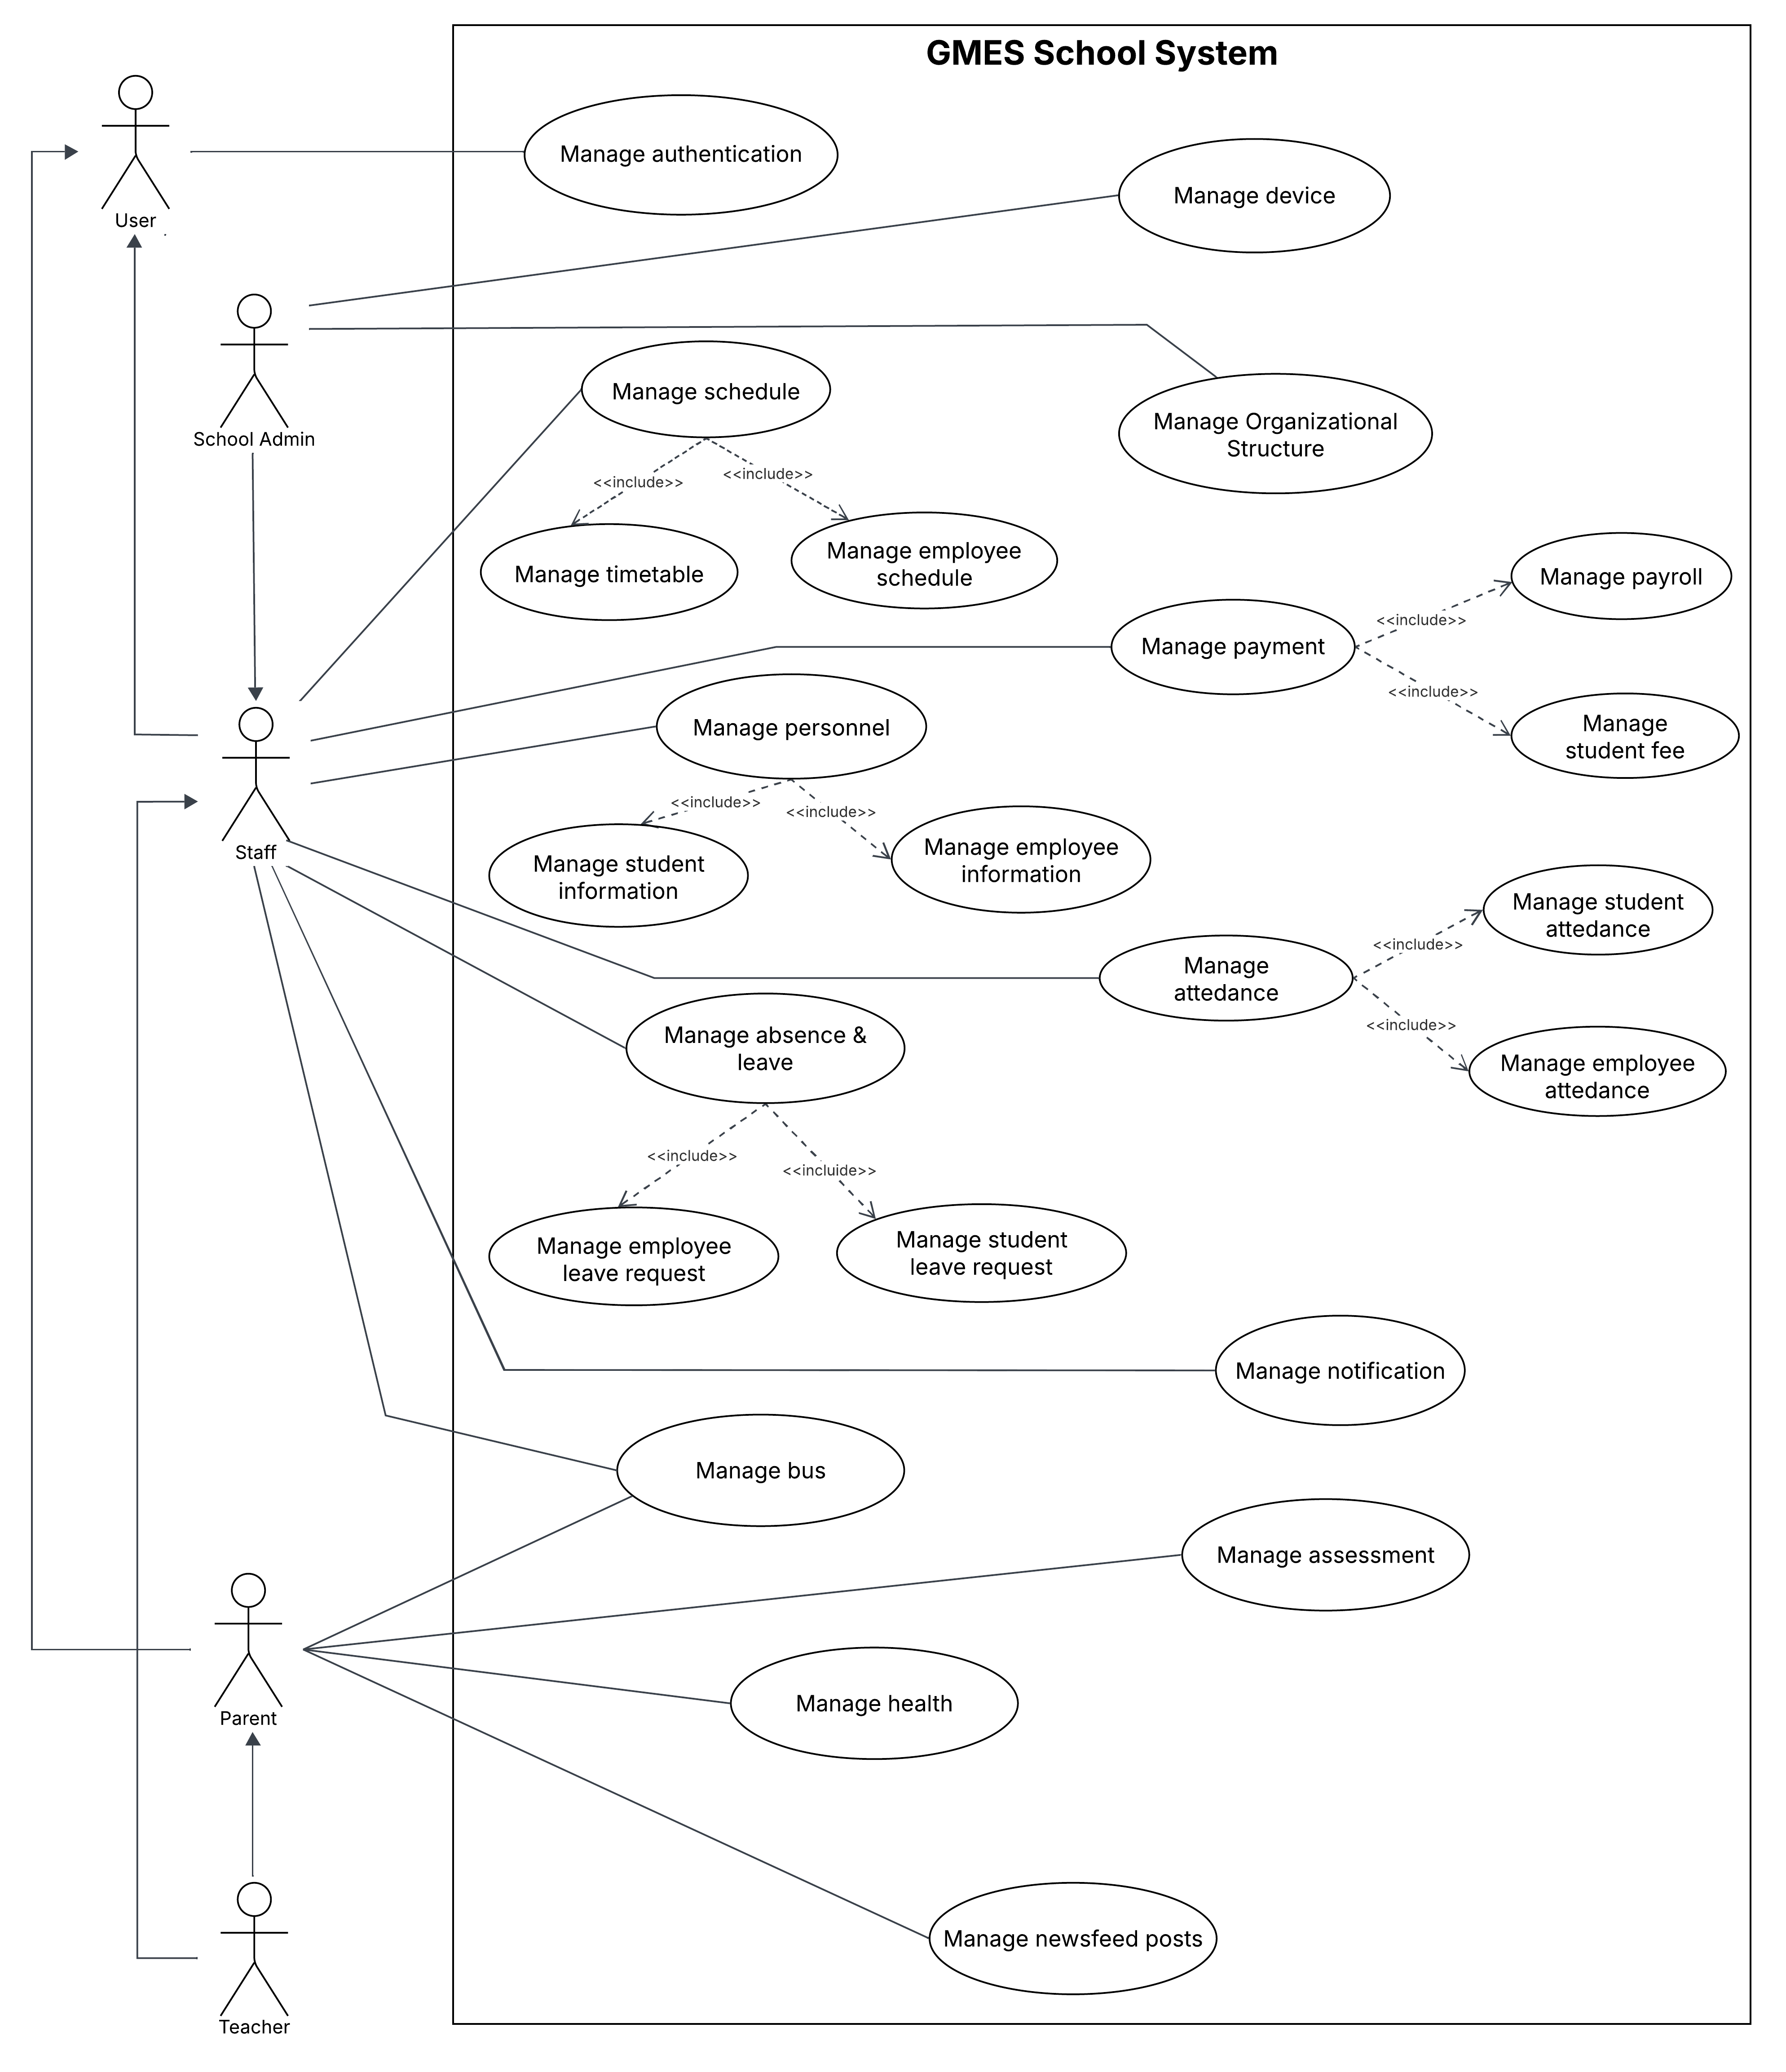
\includegraphics[width=1.1\linewidth]{images/use_case_diagram.png}
    \vspace{-2.5em}
    \caption{System requirements overview.}
    \label{fig:overview_diagram_of_usecases}
\end{figure}

\subsubsection{Detailed System Requirements}
\noindent
\begin{minipage}{\textwidth}
    \setlength{\parindent}{2em}
    This section outlines the detailed system requirements by breaking down each module into specific features. It includes a use case diagram of the \textbf{module assigned to me} and provides an analysis of its key features.
\end{minipage}
\vspace{0.5em}


% ATTENDANCE MANAGEMENT
\newpage
\indent\textbf{2.2.2.1 Attendance Management}
\begin{figure}[H]
    \centering
    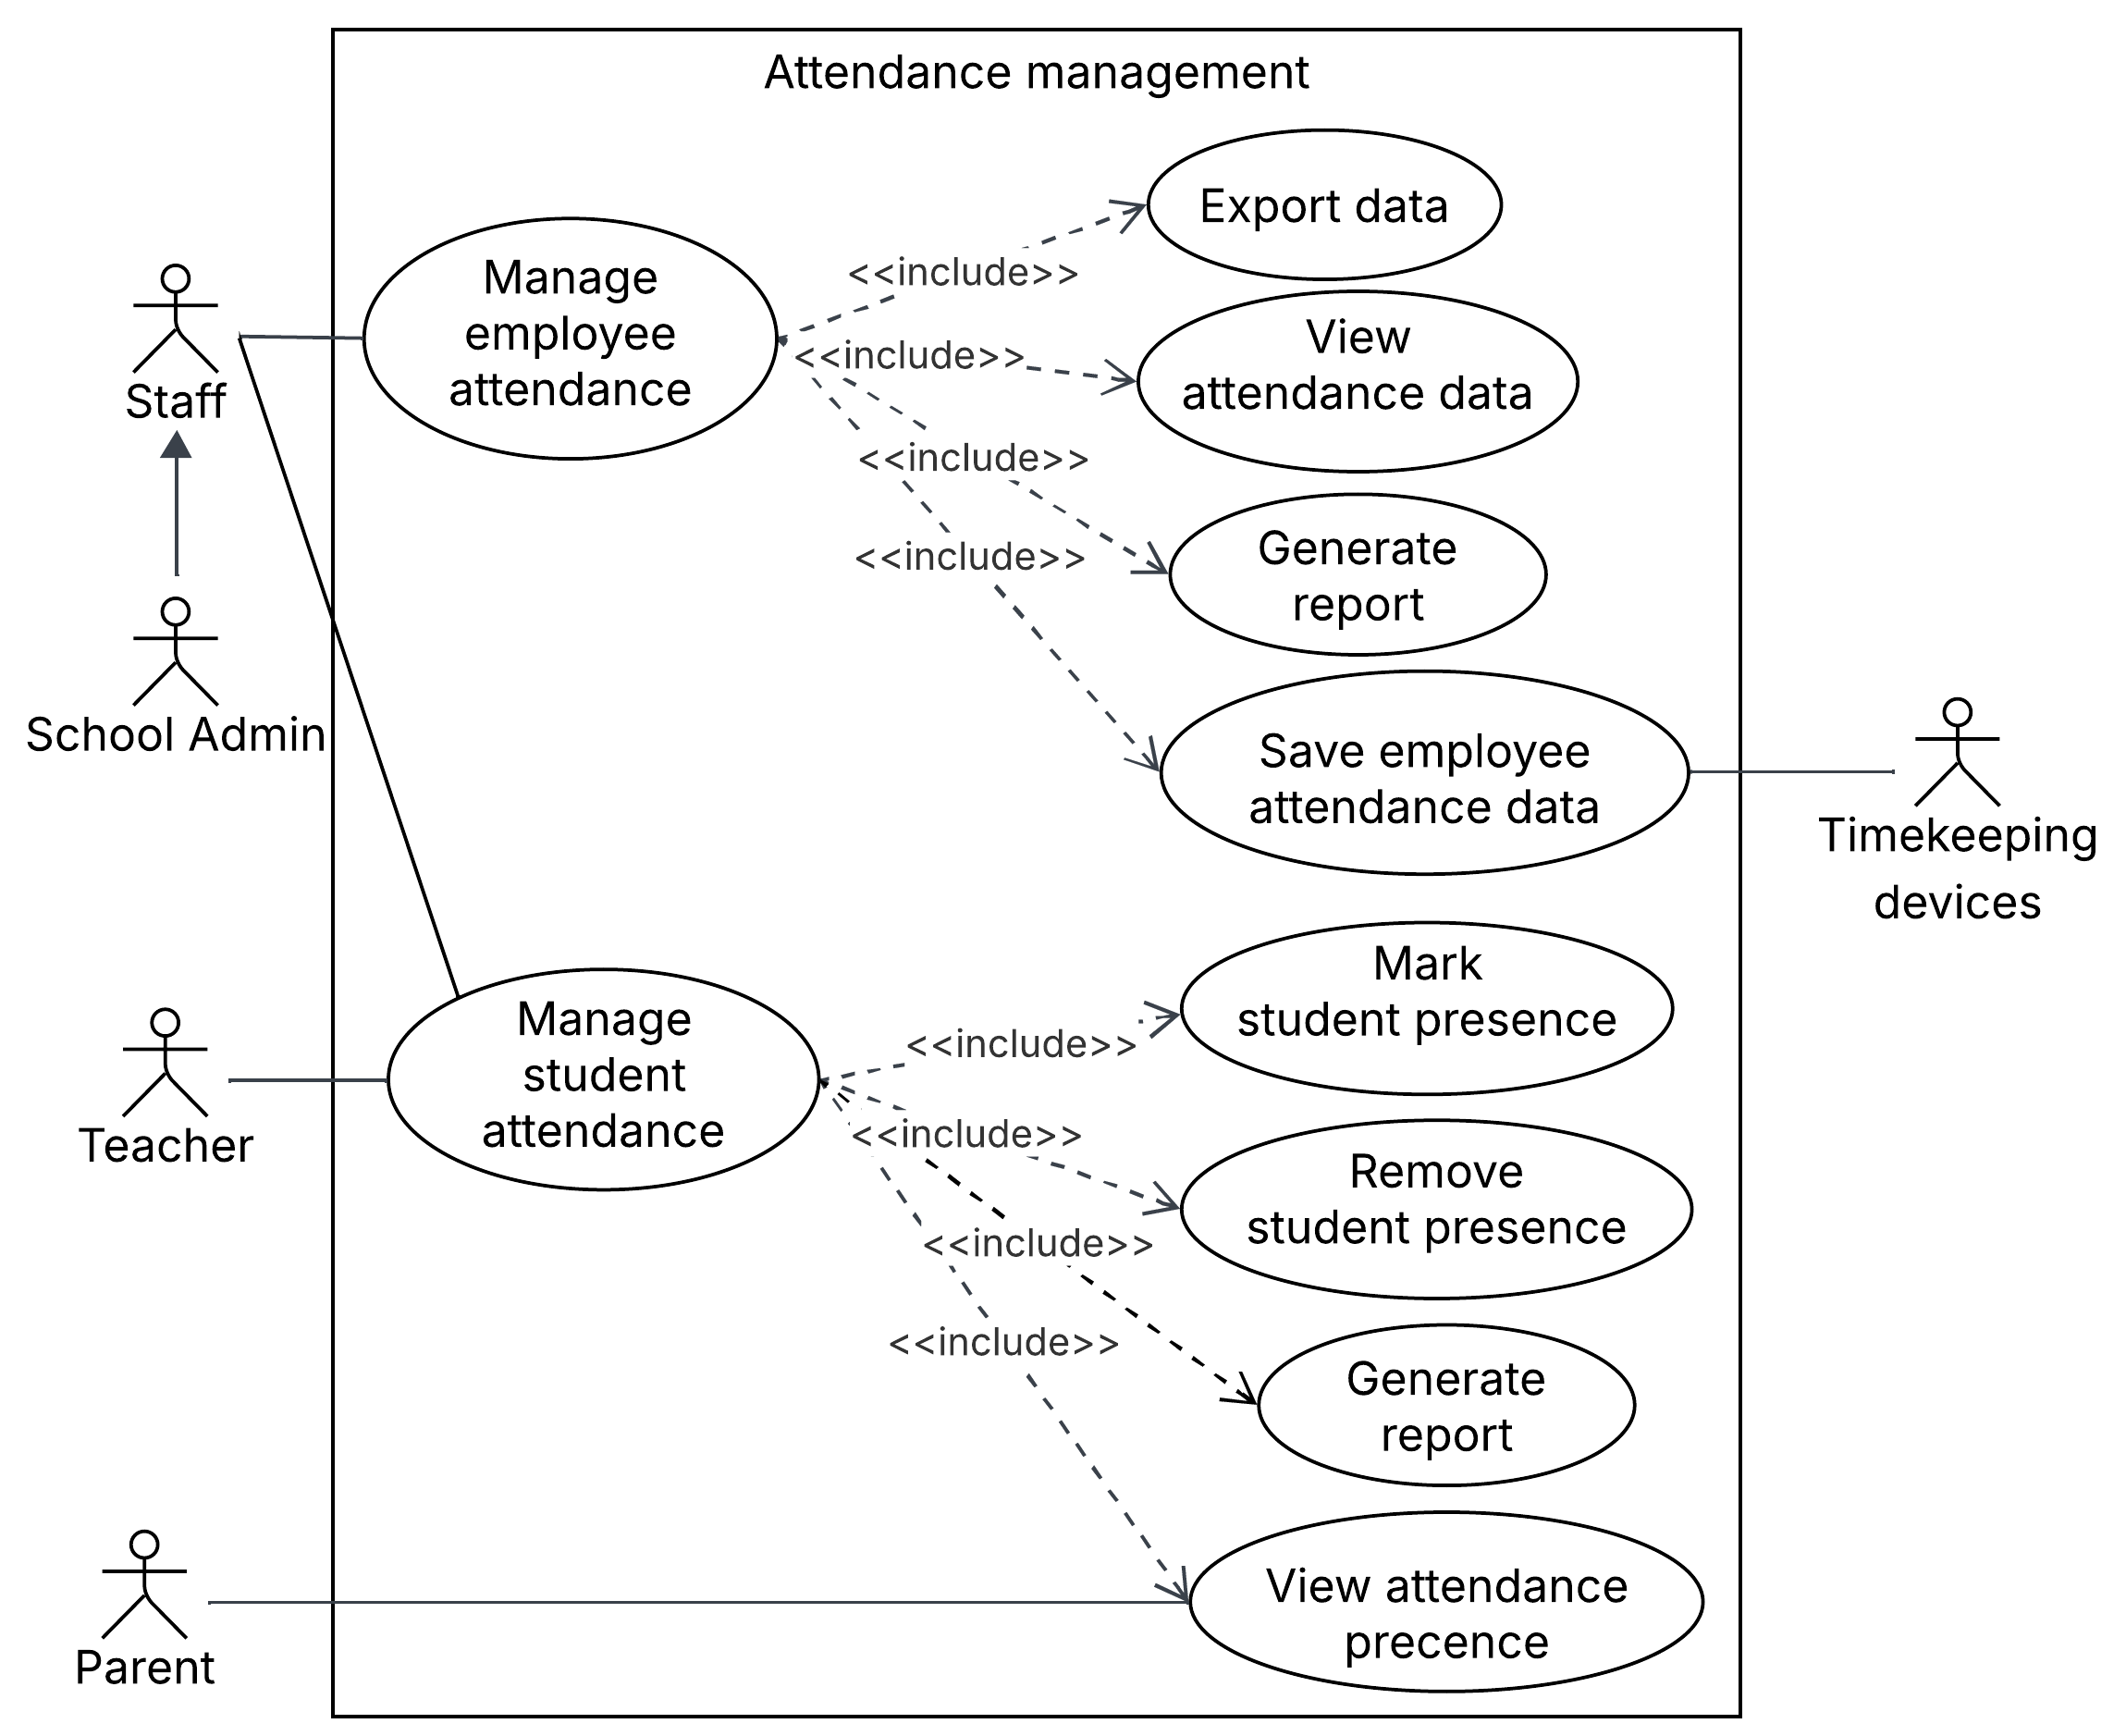
\includegraphics[width=0.7\textwidth]{images/use_case_attendance_management.png}
    \caption{Use case diagram for Attendance Management.}
    \label{fig:use_case_attendance_management}
\end{figure}
In the Attendance Management module, \textbf{the entire sub-module Student Attendance Management has been assigned to me}. The following are its key features:
\begin{itemize}[itemsep=-0.1cm, topsep=0.1cm]
    \item \textbf{Feature 1: Mark students' presence: }is a mobile app feature that enables \textbf{teachers and transportation staff} to efficiently record and update student attendance in class or on the bus with multiple status options. It ensures parents will receive notifications about their child's attendance, providing peace of mind about their safe arrival and participation.
    \item \textbf{Feature 2: Generate report: }is a web app feature that enables \textbf{administrators, authorized staff, and teachers} to create a report and export student/employee attendance data to Excel. This feature replaces manual data collection, minimizing human error, and speeding up processing time.
\end{itemize}

% ASSESSMENT MANAGEMENT
\indent\textbf{2.2.2.2 Student Assessment Management}
\begin{figure}[H]
    \centering
    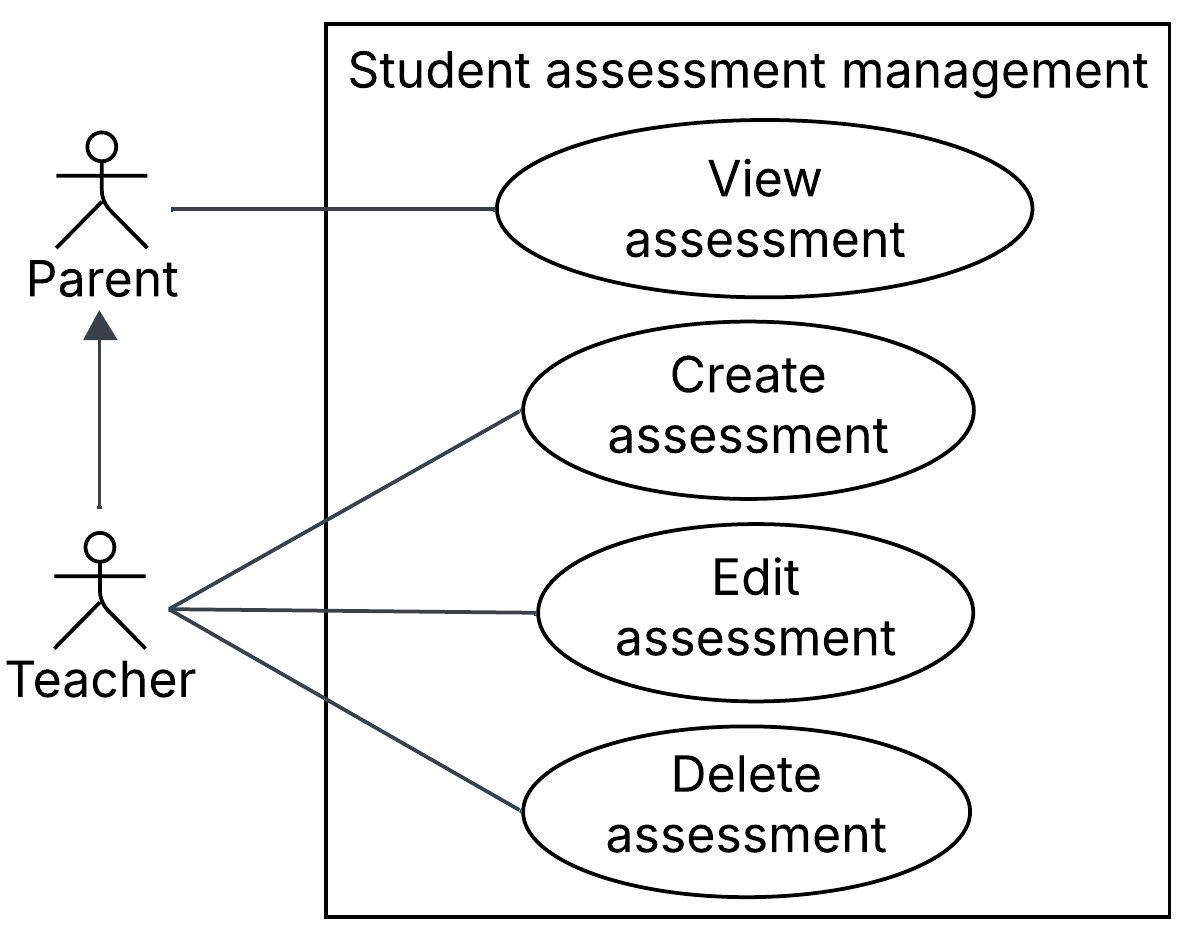
\includegraphics[width=0.4\textwidth]{images/use_case_student_assessment_management.png}
    \caption{Use case diagram for Student Assessment Management.}
    \label{fig:use_case_student_assessment_management}
\end{figure}
The \textbf{entire Student Assessment Management} module for the mobile application \textbf{has been assigned to me}. The following are its key features:
\begin{itemize}[itemsep=-0.1cm, topsep=0.1cm]
    \item \textbf{Feature 1: Create/update assessments:} allows \textbf{teachers} to create or update assessments (with file/image attachments) for their students. This feature eliminates paper-based processes, saves significant preparation time, and enhances quality through multimedia attachments.
    \item \textbf{Feature 2: View assessment:} enables \textbf{parents and teachers} monitor student progress, and performance, allowing them to identify areas where additional support may be needed and collaborate with teachers to develop appropriate solutions.
\end{itemize}

% BUS MANAGEMENT
\indent\textbf{2.2.2.3 Bus Management}
\begin{figure}[H]
    \centering
    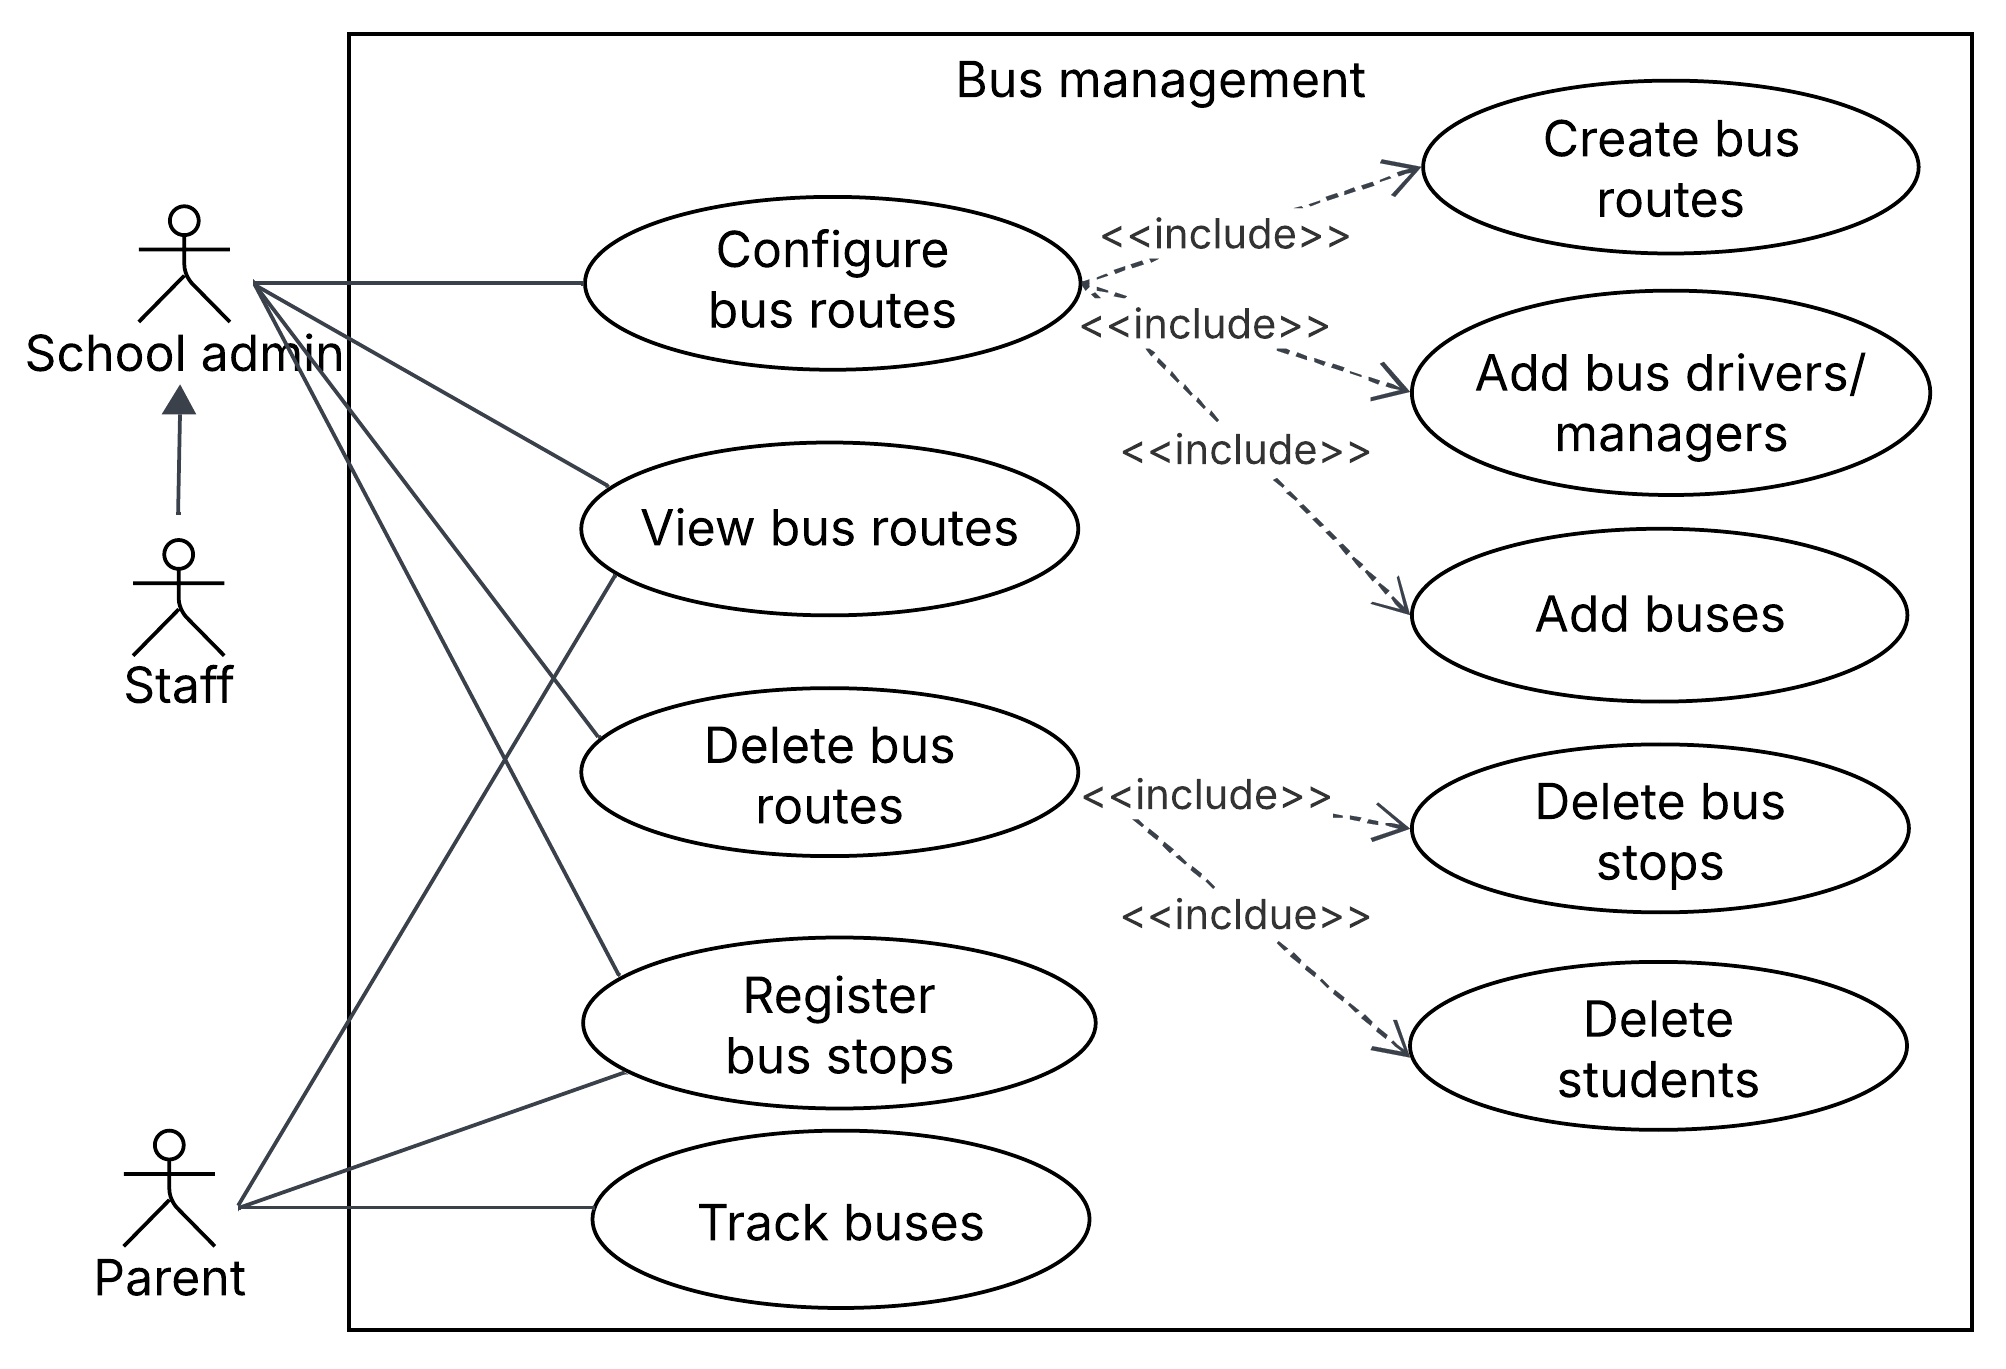
\includegraphics[width=0.7\textwidth]{images/use_case_bus_management.png}
    \caption{Use Case diagram for Bus Management.}
    \label{fig:use_case_bus_management}
\end{figure}
In the Bus Management module, the \textbf{Register Bus Stops} and \textbf{Real-Time Bus Tracking} features for mobile app are \textbf{under my responsibility}. I am also responsible for \textbf{ updating the Configure Bus Route feature} to ensure compatibility with the new Register Bus Stops module. 
\begin{itemize}[itemsep=-0.1cm, topsep=0.1cm]
    \item \textbf{Feature 1: Register bus transportation:} allows \textbf{administrators and parents} to register or cancel bus transportation services for their children. This feature saves time for both parents and staff, reduces paperwork and manual errors.
    \item \textbf{Feature 2: Track buses:} enables \textbf{parents} to monitor their children's school buses in real-time. By displaying the bus's current location, parents can track their child's journey to or from school, ensuring safety and peace of mind. This feature enhances reliability in school transportation services.
\end{itemize}

% HEALTH MANAGEMENT
\indent\textbf{2.2.2.4 Medicine Reminder Management}\\
\indent The \textbf{entire Medicine Reminder Management} module for the mobile application \textbf{has been assigned to me}. The following are its key features:
\begin{itemize}[itemsep=-0.1cm, topsep=0.1cm]
    \item \textbf{Feature 1: Create and update medicine reminder:} allows \textbf{parents} to create or update medicine reminders with image attachments to enhance reliability and clarity of medication information. It ensures that teacher are properly informed about medication schedules and dosage requirements of students.
    \item \textbf{Feature 2: Confirm medicine reminder:} enables \textbf{teachers} to confirm medicine reminder for students.
\end{itemize}
\begin{figure}[H]
    \centering
    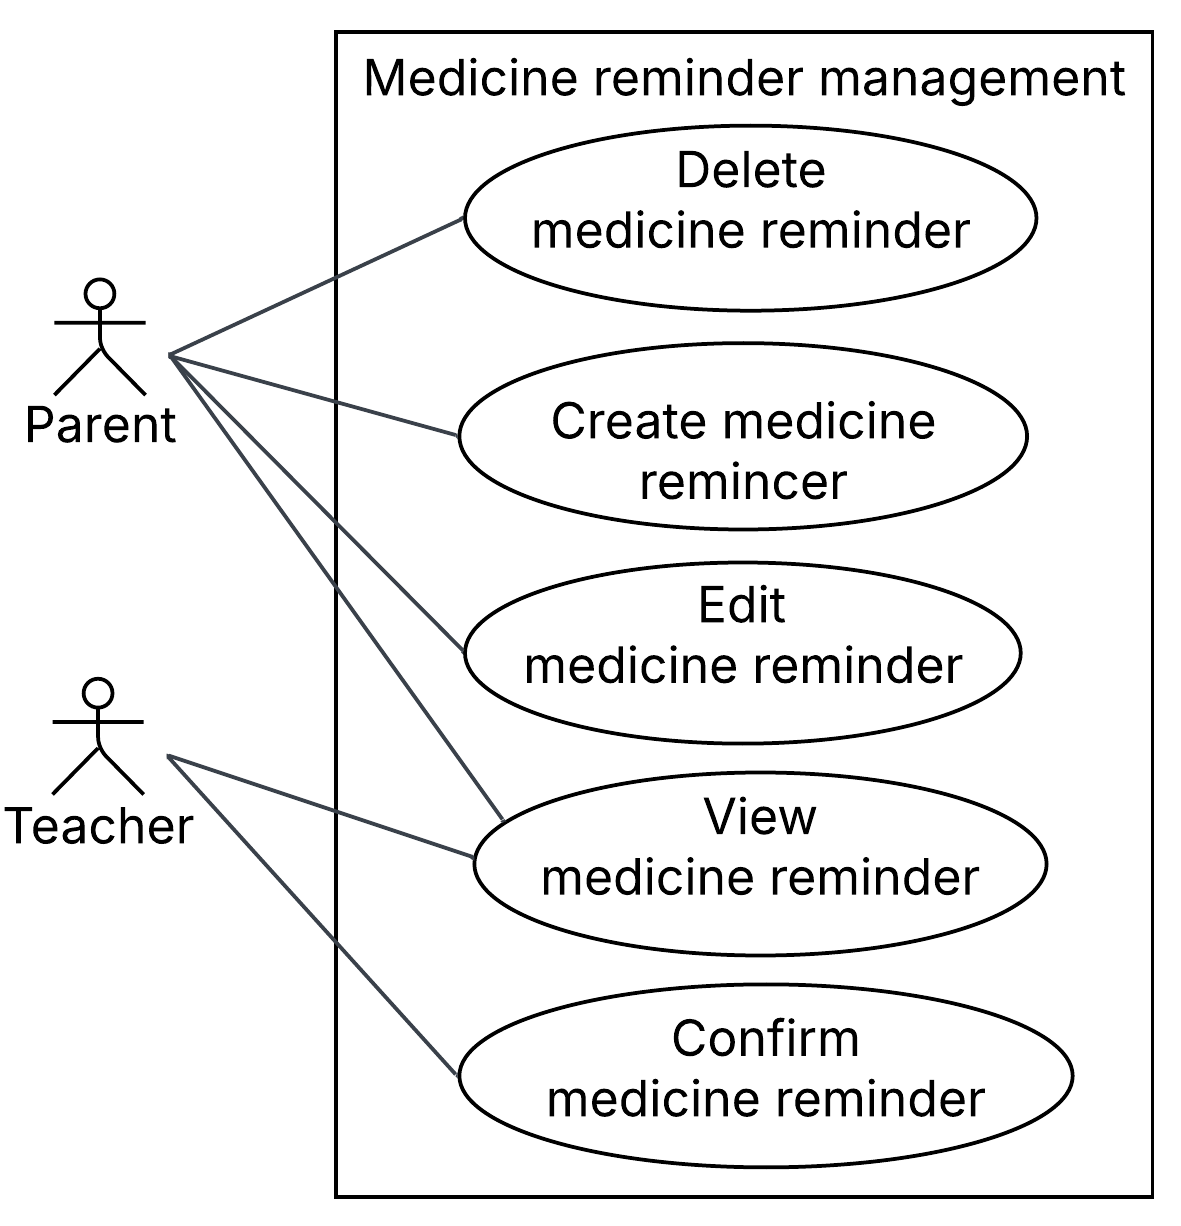
\includegraphics[width=0.45\textwidth]{images/use_case_medicine_reminder.png}
    \caption{Use case diagram for Medicine Reminder Management.}
    \label{fig:use_case_medicine_reminder_management}
\end{figure}

% LEAVE REQUEST MANAGEMENT
\indent\textbf{2.2.2.5 Leave Request Management}
\begin{figure}[H]
    \centering
    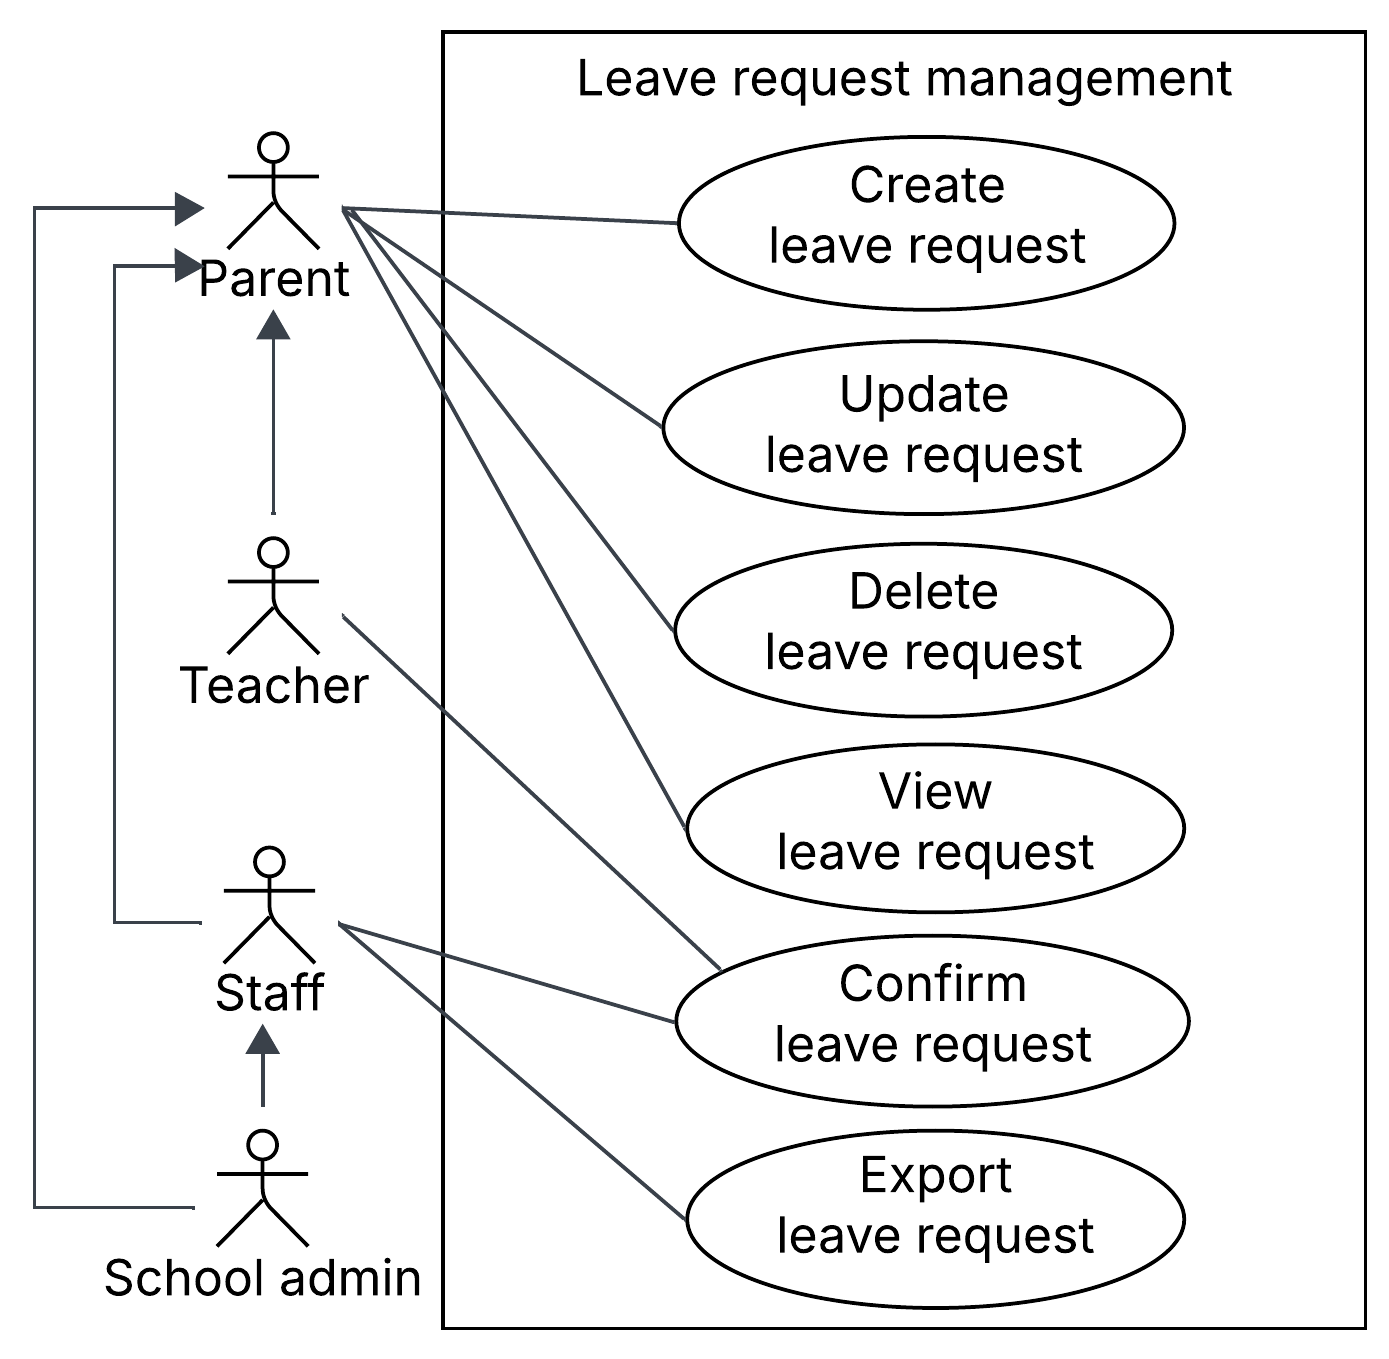
\includegraphics[width=0.5\textwidth]{images/use_case_leave_request_management.png}
    \caption{Use case diagram for Leave Request Management.}
    \label{fig:use_case_leave_request_management}
\end{figure}
Under the Leave Request Management module, the \textbf{entire sub-module Leave Request Management for Mobile App (Parents and Teachers)} is \textbf{assingned to me}. Its \textbf{key features} include the following:
\begin{itemize}[itemsep=-0.1cm, topsep=0.1cm]
    \item \textbf{Feature 1: Create and update leave request: }allows \textbf{parents and teachers} to digitally submit and manage leave requests for themselves or their students. It replaces outdated manual processes and improves transparency and compliance with institutional policies and labor regulations.
    \item \textbf{Feature 2: View and confirm leave request:}
    enables \textbf{teachers} to view their own and students' leave requests, with the ability to approve, decline, or revoke student requests. \textbf{Parents} can only track their child's leave request status.
\end{itemize}

% NEWSFEED MANAGEMENT
\indent\textbf{2.2.2.6 Newsfeed Management}
\begin{figure}[H]
    \centering
    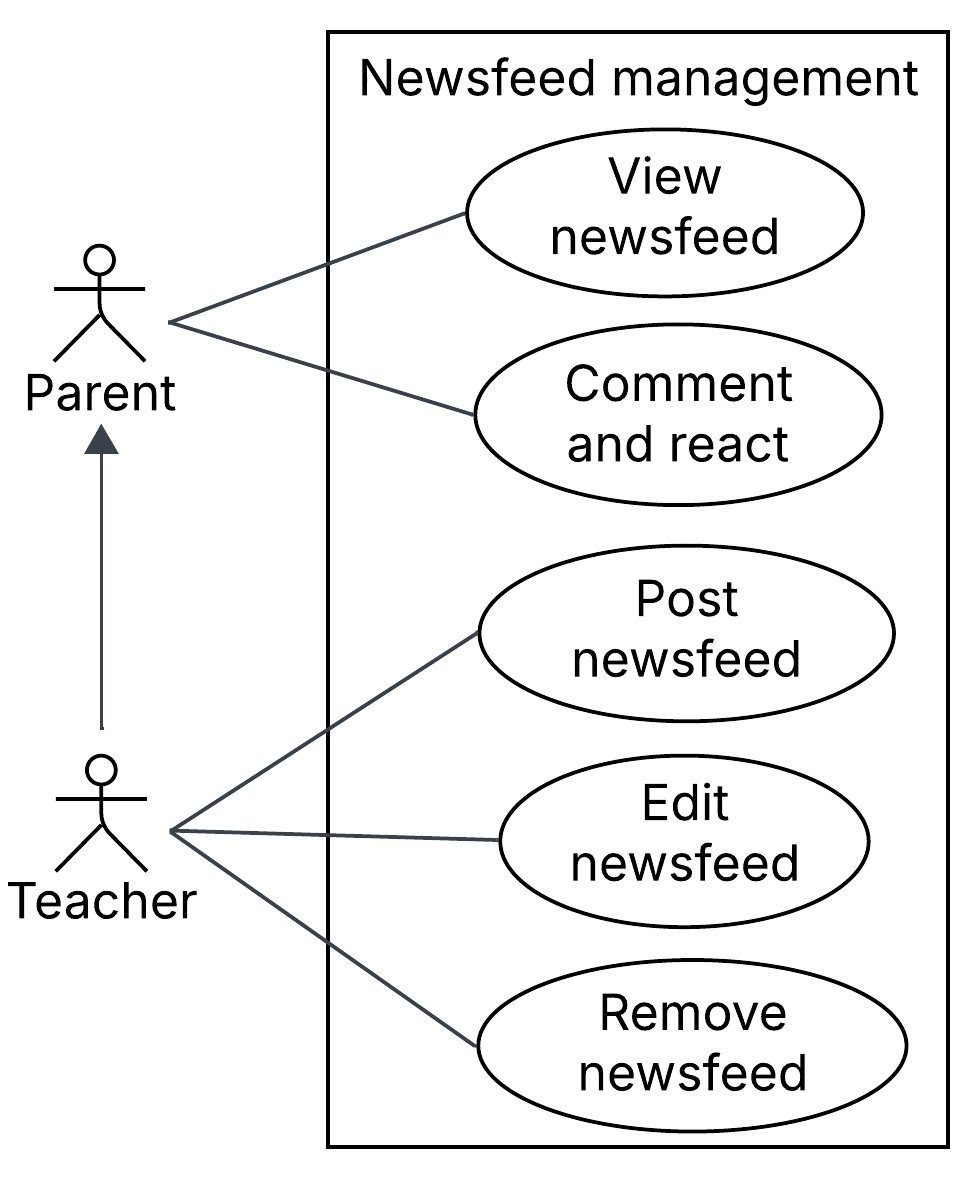
\includegraphics[width=0.35\textwidth]{images/use_case_newsfeed_management.png}
    \vspace{-0.5em}
    \caption{Use case diagram for Newsfeed Management.}
    \label{fig:use_case_newsfeed_management}
\end{figure}
The \textbf{entire Newsfeed Management module is assigned to me}. The module's \textbf{key features} include:
\begin{itemize}[itemsep=-0.1cm, topsep=0.1cm]
    \item \textbf{Feature 1: Create/update newsfeeds:} allows \textbf{teachers} to create or update posts (with file/image/video attachments) to share class events and activities with parents. This feature significantly improves communication between schools and families and ensures parents stay actively involved in their children's school life.
    \item \textbf{Feature 2: View and interact with post:} enables \textbf{parents and teachers} to view, comment on, and react to posts.
\end{itemize}

% NOTIFICATION MANAGEMENT
\indent\textbf{2.2.2.7 Notification Management}
\begin{figure}[H]
    \centering
    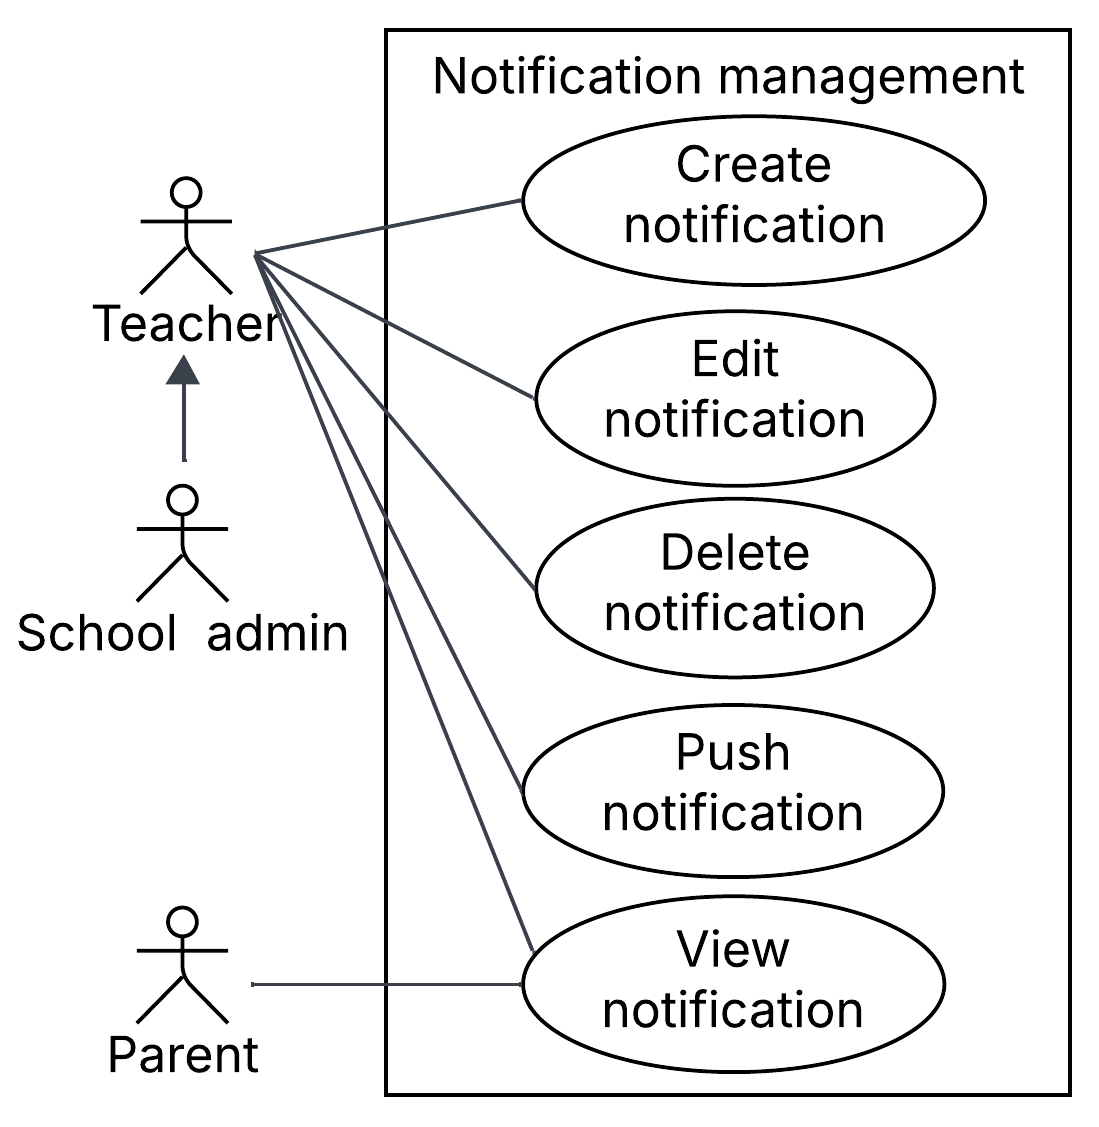
\includegraphics[width=0.4\textwidth]{images/use_case_notification_management.png}
    \caption{Use Case diagram for Notification Management.}
    \label{fig:use_case_notification_management}
\end{figure}
The \textbf{entire Notification Management module is assigned to me}. The module's \textbf{key features} include:
\begin{itemize}[itemsep=-0.1cm, topsep=0.1cm]
    \item \textbf{Feature 1: Create and push notification:} allows \textbf{administrators, authorized staff, and teachers} to create and push notifications to employees and parents through email and mobile notification channels. This feature ensures employees and parents are informed about critical notifications, events, and important updates.
\end{itemize}

% PERSONNEL MANAGEMENT
\indent\textbf{2.2.2.8 Personnel management}
\begin{figure}[H]
    \centering
    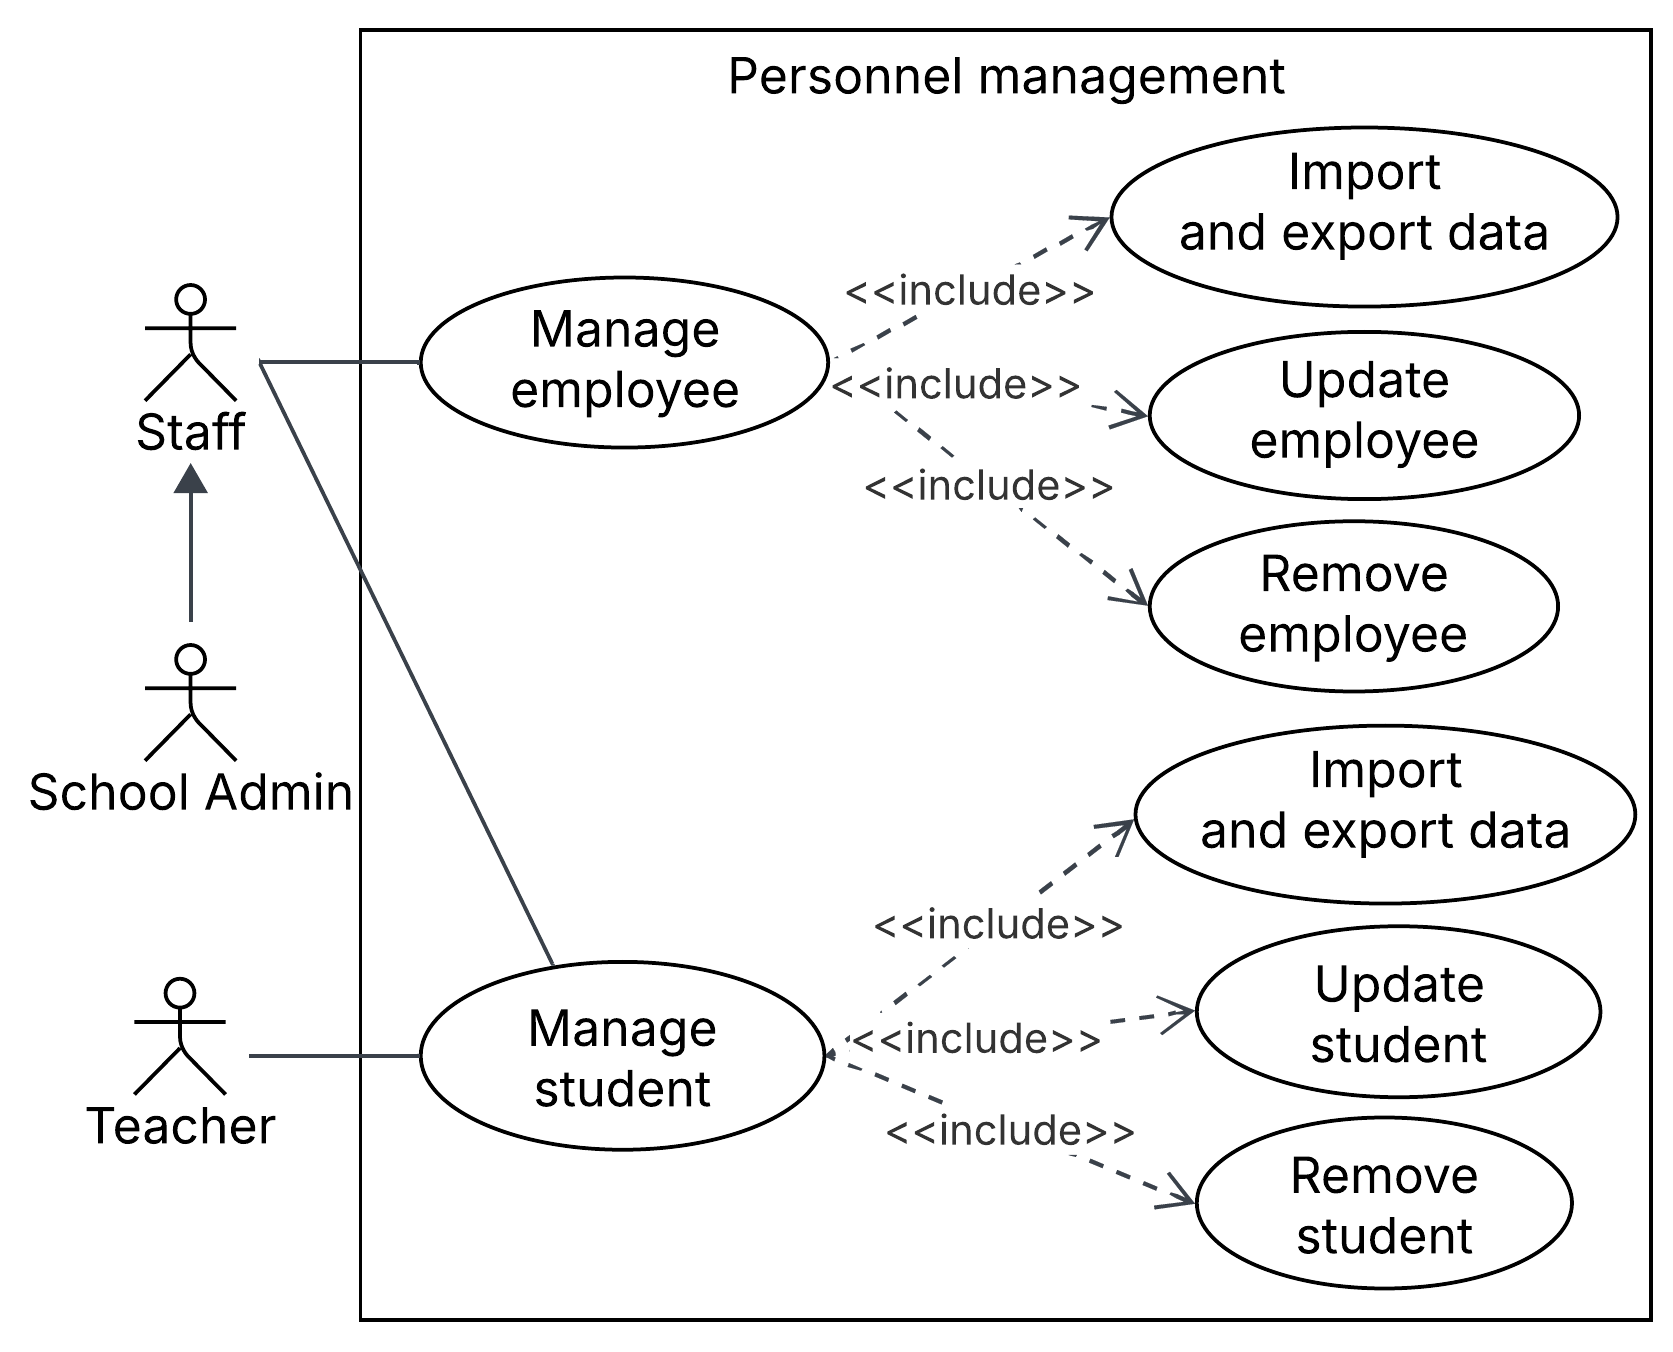
\includegraphics[width=0.6\textwidth]{images/use_case_personnel_management.png}
    \caption{Use case diagram for Personnel Management.}
    \label{fig:use_case_personnel_management}
\end{figure}
Under the the Personnel Management module, my responsibilities include developing the \textbf{Import/Export} functionality for employee and student data.
\begin{itemize}[itemsep=-0.1cm, topsep=0.1cm]
    \item \textbf{Feature 1: Import employee/student data: }allows \textbf{administrators and authorized staff} to efficiently create and update multiple employee/student data into the system, via Excel or ERP. This feature significantly reduces time, and effort and minimizes errors.
    \item \textbf{Feature 2: Export employee/student data: }allows \textbf{administrators and authorized staff} to export employee/student data to Excel for reporting purposes.
\end{itemize}

  % 2.3 Non-functional Requirements
  % \subsection{Non-functional Requirements}
  % \indent

  In this system, the following non-functional requirements make the system more comprehensive, improve user experience, and ensure secure, reliable operation while improving performance and usability standards: 
\begin{itemize}[itemsep=-0.1cm, topsep=0.1cm]
    \item The system must be compatible with the most popular browsers/platforms currently available.
    \item The system must ensure data security and privacy of user information.
    \item The system must have a user-friendly interface, easy to use to enable interaction without encountering too many difficulties.
    \item The system response time must be fast and stable.
    \item The system must remain stable to operate efficiently even during high-access traffic.
    \item The system needs to have periodic data backups to ensure security and the ability to recover data when necessary.
\end{itemize}

  % 2.4 Use case diagram
  % \subsection{Use-case Diagram}
  % \indent

% This section presents the high-level use case diagram of the system along with detailed visualizations of use cases. It provides a comprehensive view of system functionality, beginning with the big-picture interactions before focusing on specific use cases \textbf{under our responsibility}.
% \subsubsection{Overview diagram of usecases}
% \noindent
% \begin{minipage}{\textwidth}
%     \setlength{\parindent}{2em}
%     From the system requirements and user roles, we analyzed key interactions and designed an overview diagram of use cases to visualize the system's core functionalities. This diagram provides a clear, high-level overview of how users interact with the GMES system.
% \end{minipage}

% \begin{figure}[H]
%     \centering
%     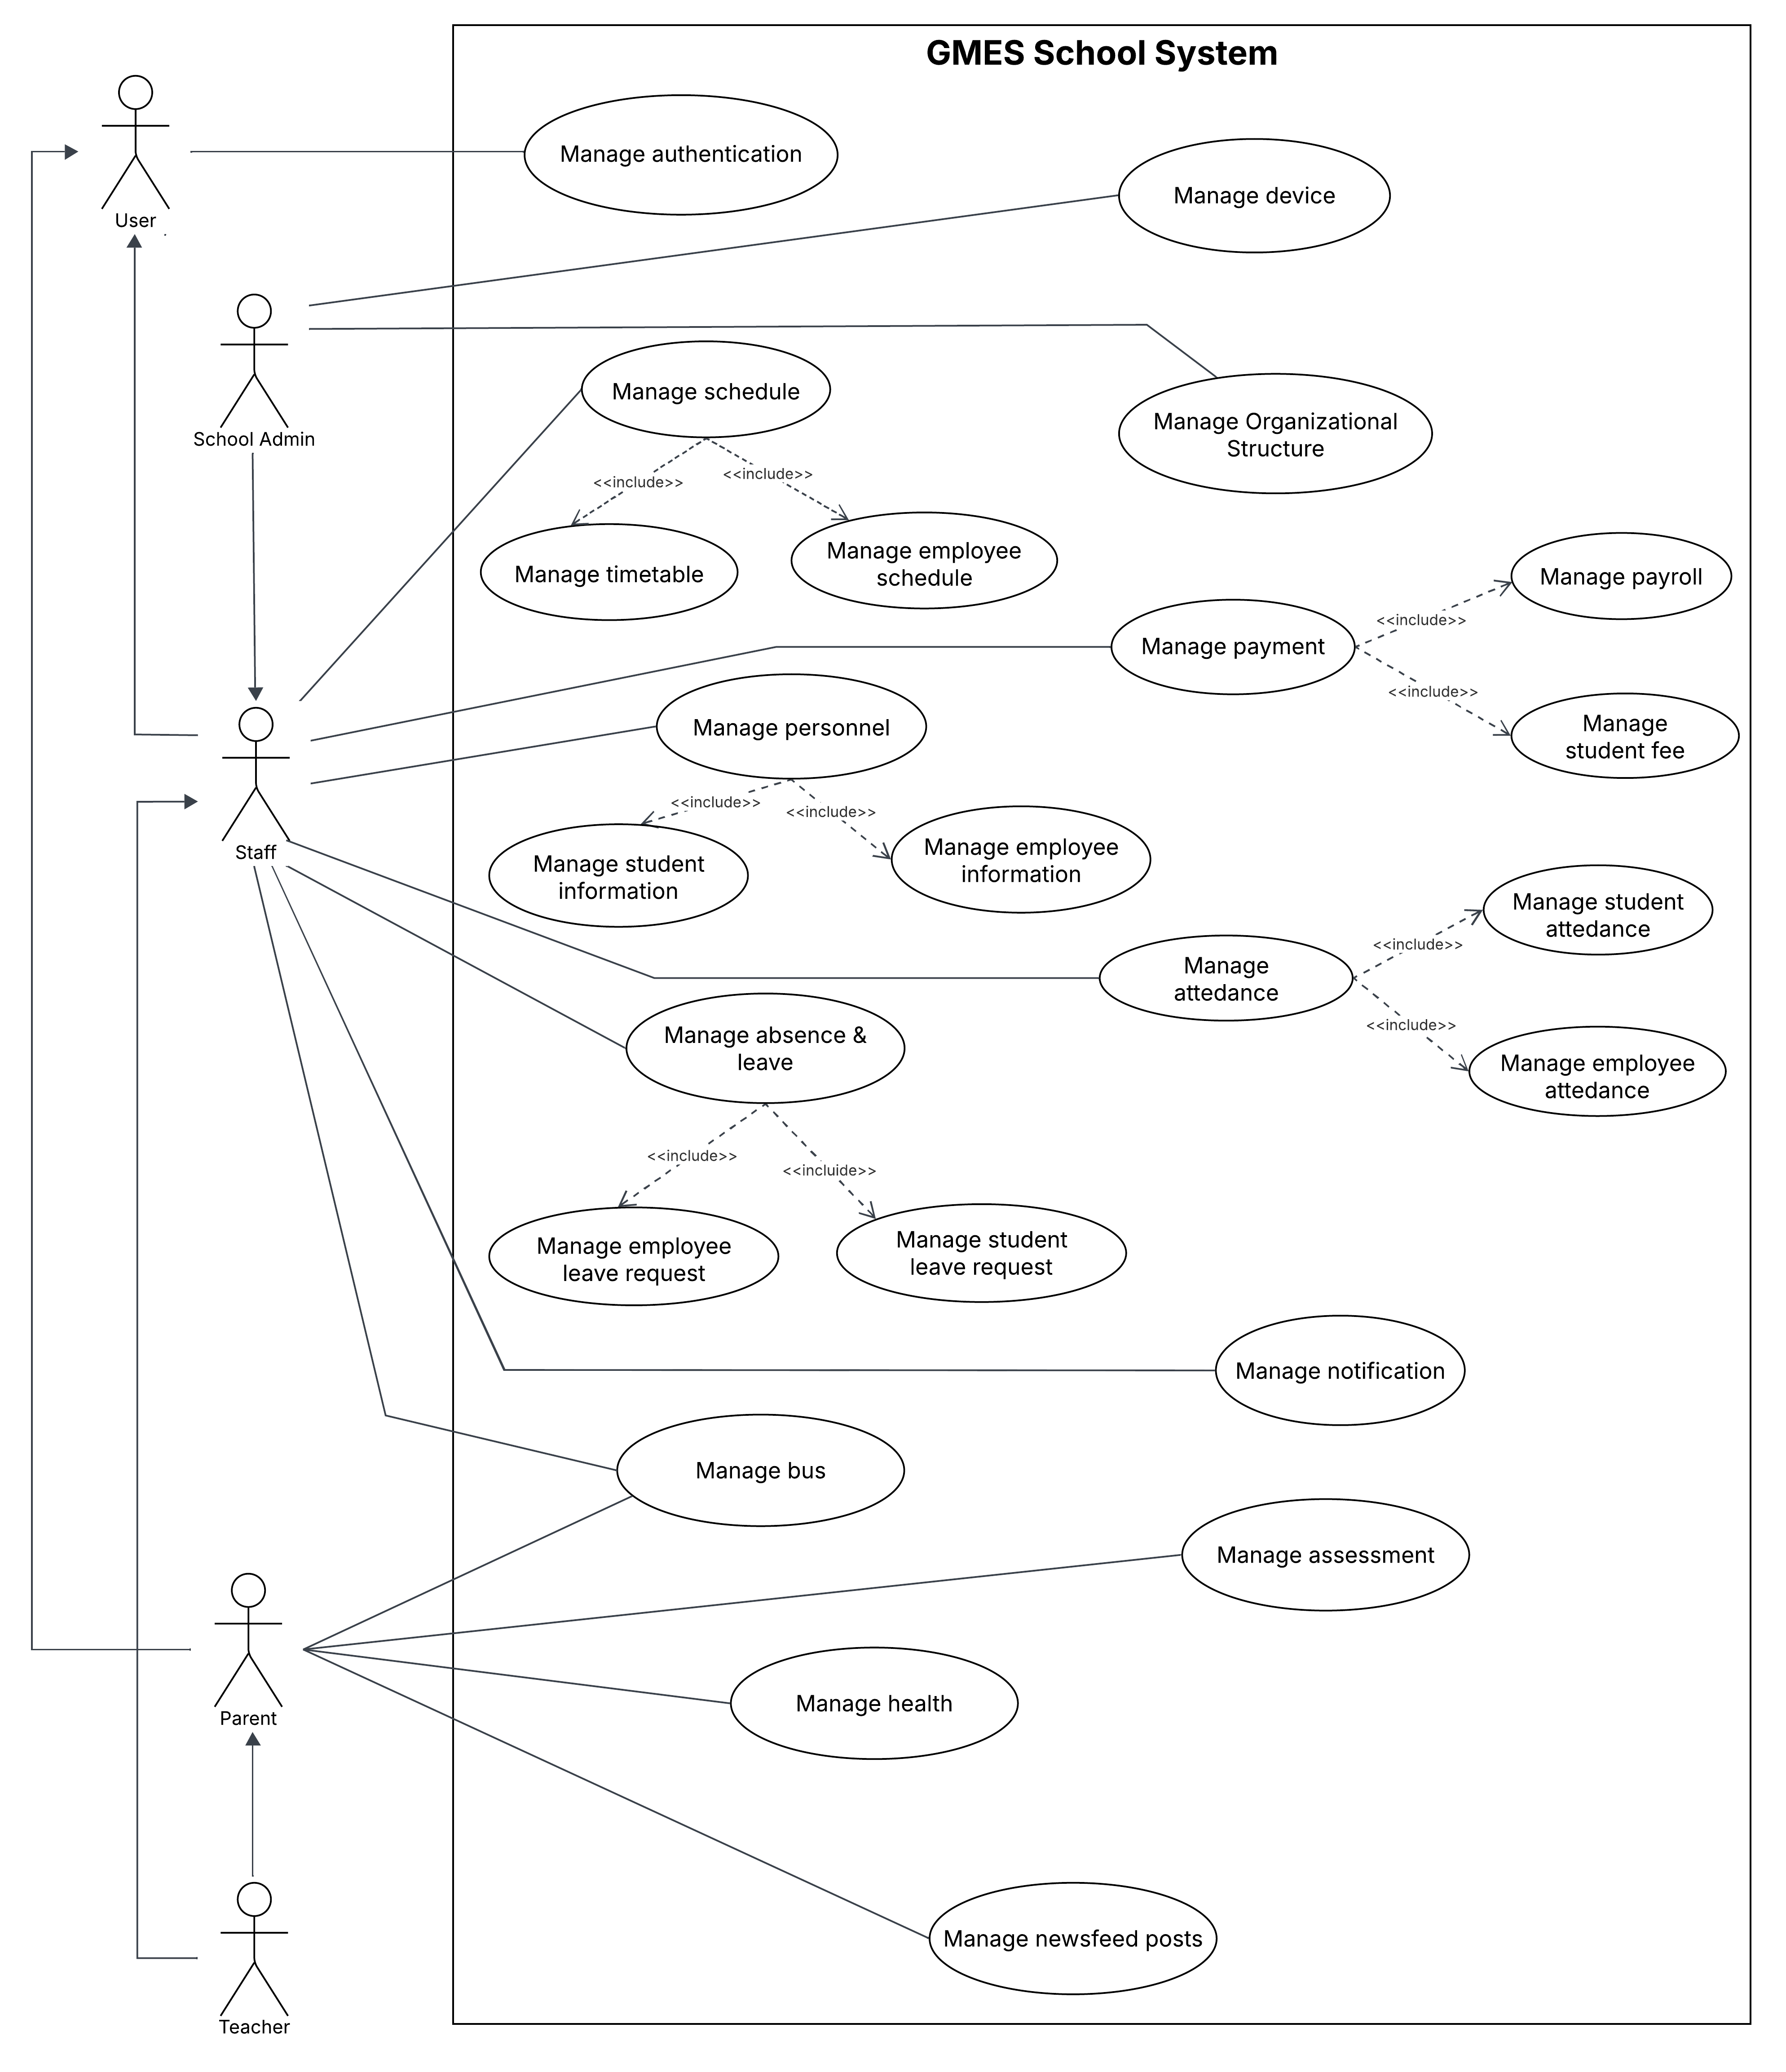
\includegraphics[width=1.1\linewidth]{images/use_case_diagram.png}
%     \vspace{-2.5em}
%     \caption{Overview diagram of use cases.}
%     \label{fig:overview_diagram_of_usecases}
% \end{figure}

\subsubsection{Detailed Use Case Diagrams}
\noindent
\begin{minipage}{\textwidth}
    \setlength{\parindent}{2em}
    While the previous section provided an overview of the system's functionalities, \textbf{this section presents detailed use case diagrams for each function under our responsibility} within the GMES School system. These diagrams illustrate the specific interactions between user roles and system features.
\end{minipage}
\vspace{0.5em}

% % AUTHENTICATION
% \indent\indent\textbf{2.4.2.1 Authentication usecase diagram}
% \vspace{0.5em}
% \par\indent\indent\parbox{0.9\textwidth}{
%     The Authentication function allow all users which use the GMES School system to securely access or exit the system.
% }
% \begin{figure}[H]
%     \centering
%     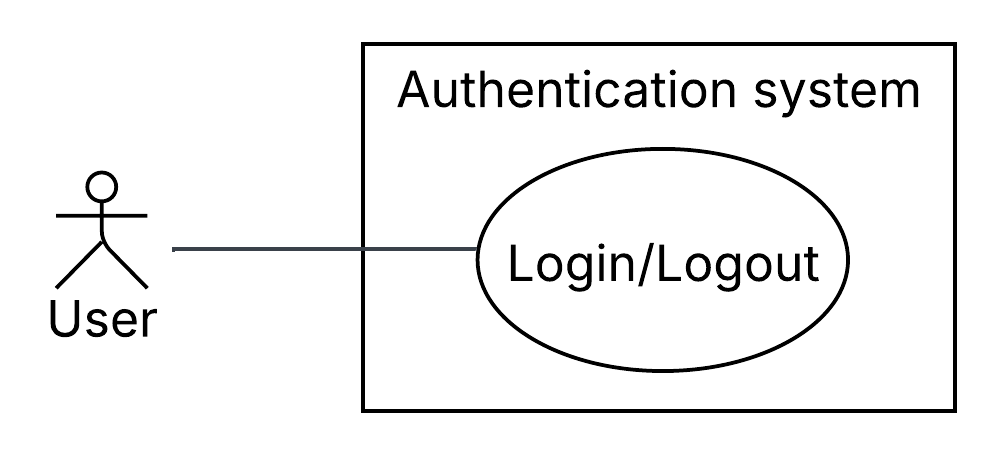
\includegraphics[width=0.6\textwidth]{images/use_case_login_logout.png}
%     \caption{Usecase diagram for login/logout.}
%     \label{fig:use_case_login_logout}
% \end{figure}

% PERSONNEL MANAGEMENT
% \newpage
% \indent\indent\textbf{2.4.2.1 Personnel Management Use Case Diagram}
% \vspace{0.5em}
% \par\indent\indent\parbox{0.9\textwidth}{
%     \setlength{\parindent}{2em}The Personnel Management module allows staff, school administrators, and teachers to manage personnel information. Staff and school administrators can manage employees, and students under their supervision, while teachers can only manage students under their supervision. This role-based approach prevents unauthorized access to sensitive information such as salary details, personal contracts, and student records, ensuring only authorized users can view or edit them. It also keeps information accurate by giving the right permissions to the right people.
% }\\
% \begin{figure}[H]
%     \centering
%     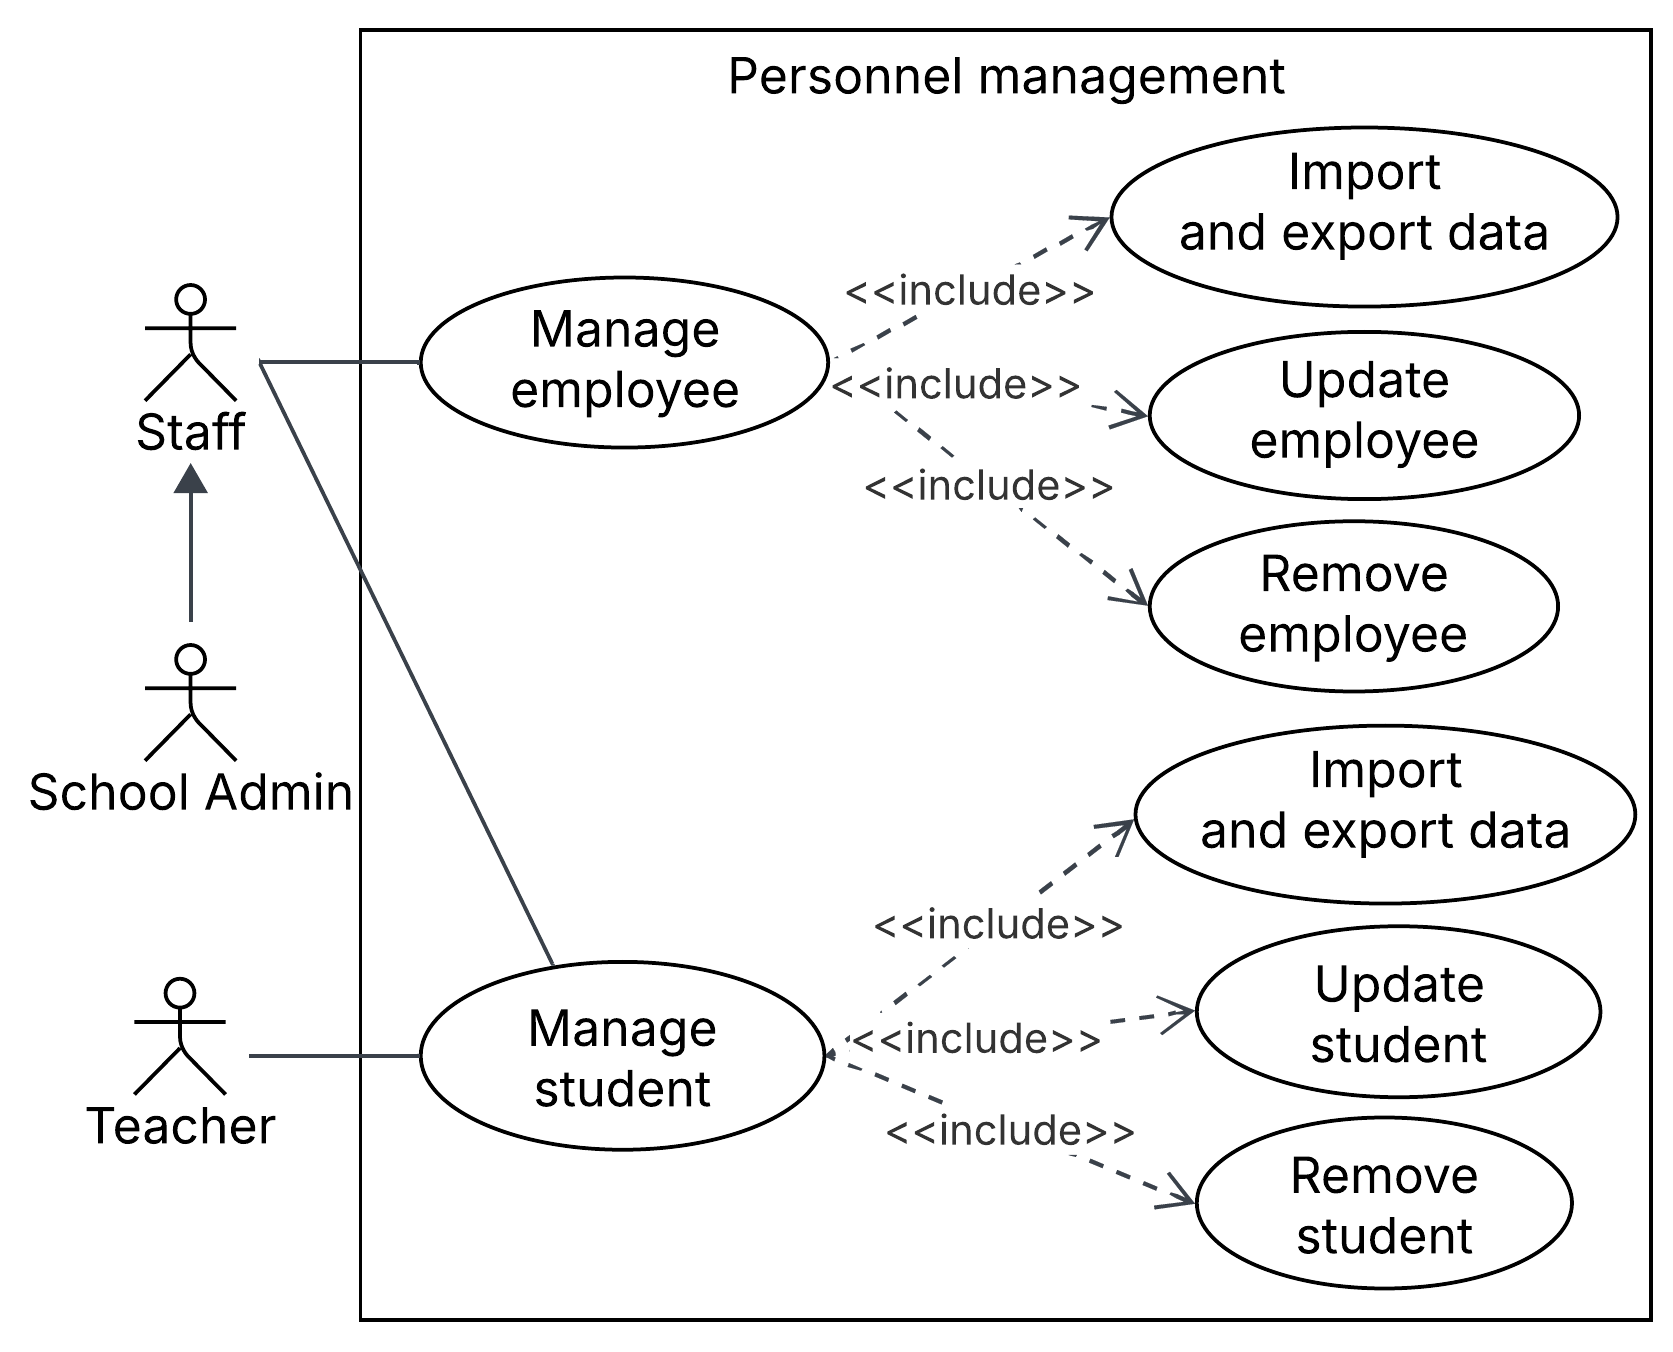
\includegraphics[width=0.7\textwidth]{images/use_case_personnel_management.png}
%     \caption{Use case diagram for Personnel Management.}
%     \label{fig:use_case_personnel_management}
% \end{figure}

% PERSONNEL MANAGEMENT: IMPORT EMPLOYEE DATA
% \renewcommand{\arraystretch}{1.5}
% \begin{longtable}{|>{\raggedright\arraybackslash}p{3.5cm}|
%                   >{\raggedright\arraybackslash}p{10cm}|}
% \caption{Import employee data via Excel basic flow.}
% \label{tab:employee_management_basic_flow} \\
% \endfirsthead
% \endhead
% \hline
%     \textbf{Function name} & \textbf{Import employee data}\\
%     \hline
%     Actor & Administrators and staff \\
%     \hline
%     Description & Support administrators and staff to import employee data to the database via Excel file \\
%     \hline
%     Pre-conditions & {
%         \vspace{-1.7em}
%         \begin{itemize}
%             \item The administrators and staff must log into the system with valid access rights
%             \vspace{-0.8em}
%             \item The uploaded file must be Excel file (.xlsx/.xls).
%             \vspace{-1.5em}
%         \end{itemize}    
%     }\\
%     \hline
%     Main flow &  {
%         \vspace{-1.7em}
%         \begin{itemize}
%             \item The administrators and staff access the Employee profiles feature.
%             \vspace{-0.8em}
%             \item The system gets the departments which are managed by the user (displayed in a tree structures).
%             \vspace{-0.8em}
%             \item Users select a department and uploaded the Excel file.
%             \vspace{-0.8em}
%             \item System validate the data in the uploaded file and save it to database.
%             \vspace{-0.8em}
%             \item Finish the process of importing employees data.
%             \vspace{-1.8em}
%         \end{itemize}    
%     }\\
%     \hline
% \end{longtable}

% ATTENDANCE MANAGEMENT
% \indent\indent\textbf{2.4.2.2 Attendance Management Use Case Diagram}
% \vspace{0.5em}
% \begin{adjustwidth}{3em}{0em}
%     \setlength{\parindent}{2em}
%     \leavevmode\indent
%     The Attendance Management module allows staff and school administrators to manage the attendance records of employees under their supervision, while teachers and school administrators can manage the attendance records of students under their supervision. Additionally, a parent can also view the attendance records of their child. For employees, attendance data is automatically recorded by timekeeping devices or it can be updated by the administrators and stored in the database. For students, attendance data is stored when the teacher marks the presence in class. This module will help organizations track the check-in/check-out time of employees to calculate their salary. It also improves communication between teacher and parent by sending notifications when teachers mark student attendance, giving parents better oversight of their child.
% \end{adjustwidth}    
% \begin{figure}[H]
%     \centering
%     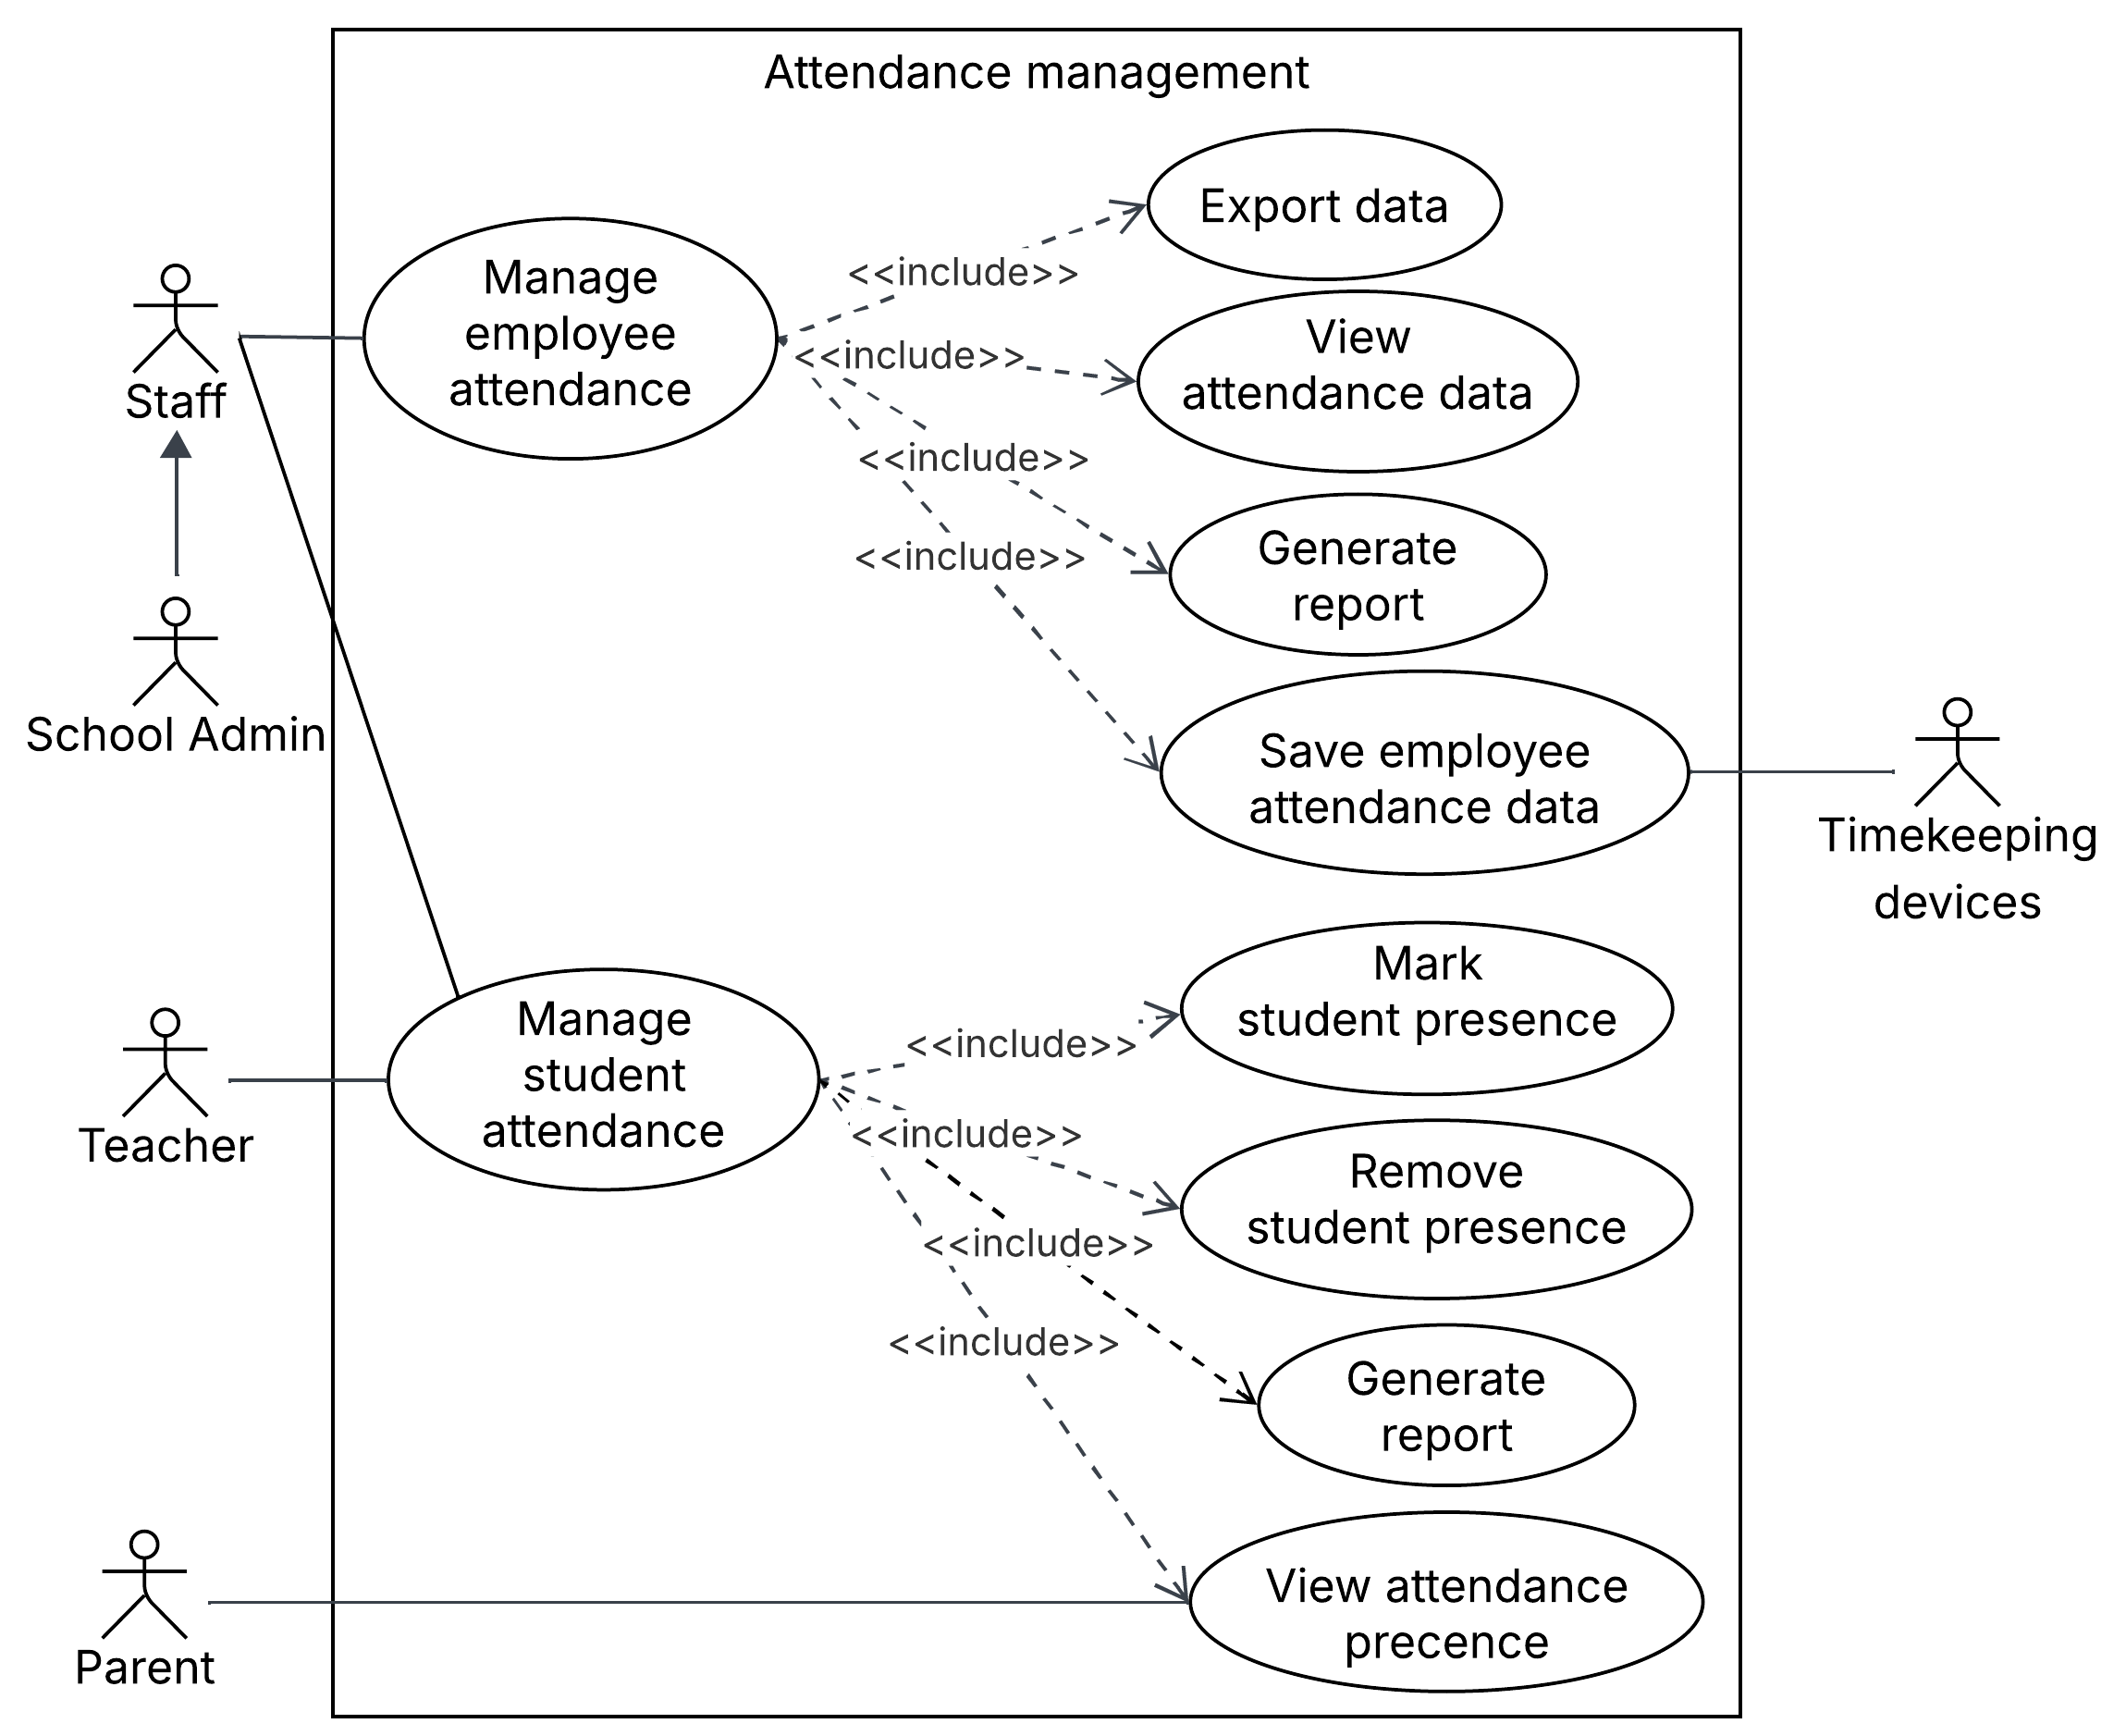
\includegraphics[width=\textwidth]{images/use_case_attendance_management.png}
%     \caption{Use case diagram for Attendance Management.}
%     \label{fig:use_case_attendance_management}
% \end{figure}

% ATTENDANCE MANAGEMENT: MARK ATTENDANCE IN CLASS
% \renewcommand{\arraystretch}{1.5}
% \begin{longtable}{|>{\raggedright\arraybackslash}p{3.5cm}|
%                   >{\raggedright\arraybackslash}p{10cm}|}
% \caption{Use Case Analysis for the Student Attendance Feature in Class.}
% \label{tab:attendance_management_student_attendance} \\
% \endfirsthead
% \endhead
% \hline
%     \textbf{Function name} & \textbf{Mark student attendance in class}\\
%     \hline
%     Actor & Teachers \\
%     \hline
%     Description & Support teachers to record student attendance when students arrive at class and when they leave to go home. \\
%     \hline
%     Pre-conditions & {
%         \vspace{-1.7em}
%         \begin{itemize}
%             \item The administrators and teachers must log into the system with valid access rights
%             \vspace{-0.8em}
%             \item The teachers must manage at least one class.
%             \vspace{-1.5em}
%         \end{itemize}    
%     }\\
%     \hline
%     Main flow &  {
%         \vspace{-1.7em}
%         \begin{itemize}
%             \item Teachers selects a class and access the Attendance feature
%             \vspace{-0.8em}
%             \item The system retrieves a list of students with their current status (checked/unchecked).
%             \vspace{-0.8em}
%             \item Teacher selects student and mark attendance status.
%             \vspace{-0.8em}
%             \item System save the records and push notification to parents.
%             \vspace{-0.8em}
%             \item Finish the process of marking student attendance data.
%             \vspace{-1.8em}
%         \end{itemize}    
%     }\\
%     \hline
% \end{longtable}

% LEAVE REQUEST MANAGEMENT
% \indent\indent\textbf{2.4.2.3 Leave Request Management Use Case Diagram}
% \vspace{0.5em}
% \begin{adjustwidth}{3em}{0em}
%     \setlength{\parindent}{2em}
%     \leavevmode\indent 
%     The Leave Request Management module enables school administrators, staff, teachers and parents to create, update, delete, and view leave requests. Parents can only manage leave requests for their own children, while teachers can manage their own requests and have the ability to review and confirm leave requests for students under their supervision. Staff and school administrators can manage leave requests for employees they supervise, including actions such as approving, declining, or canceling confirmed leave requests. Additionally, they can also export the leave request data of employees under their supervision to an Excel file. This module will reduce paperwork and manual errors in tracking absences. It also provides a clear working flow for requesting, reviewing, and approving or declining leave requests.
% \end{adjustwidth}   
% \begin{figure}[H]
%     \centering
%     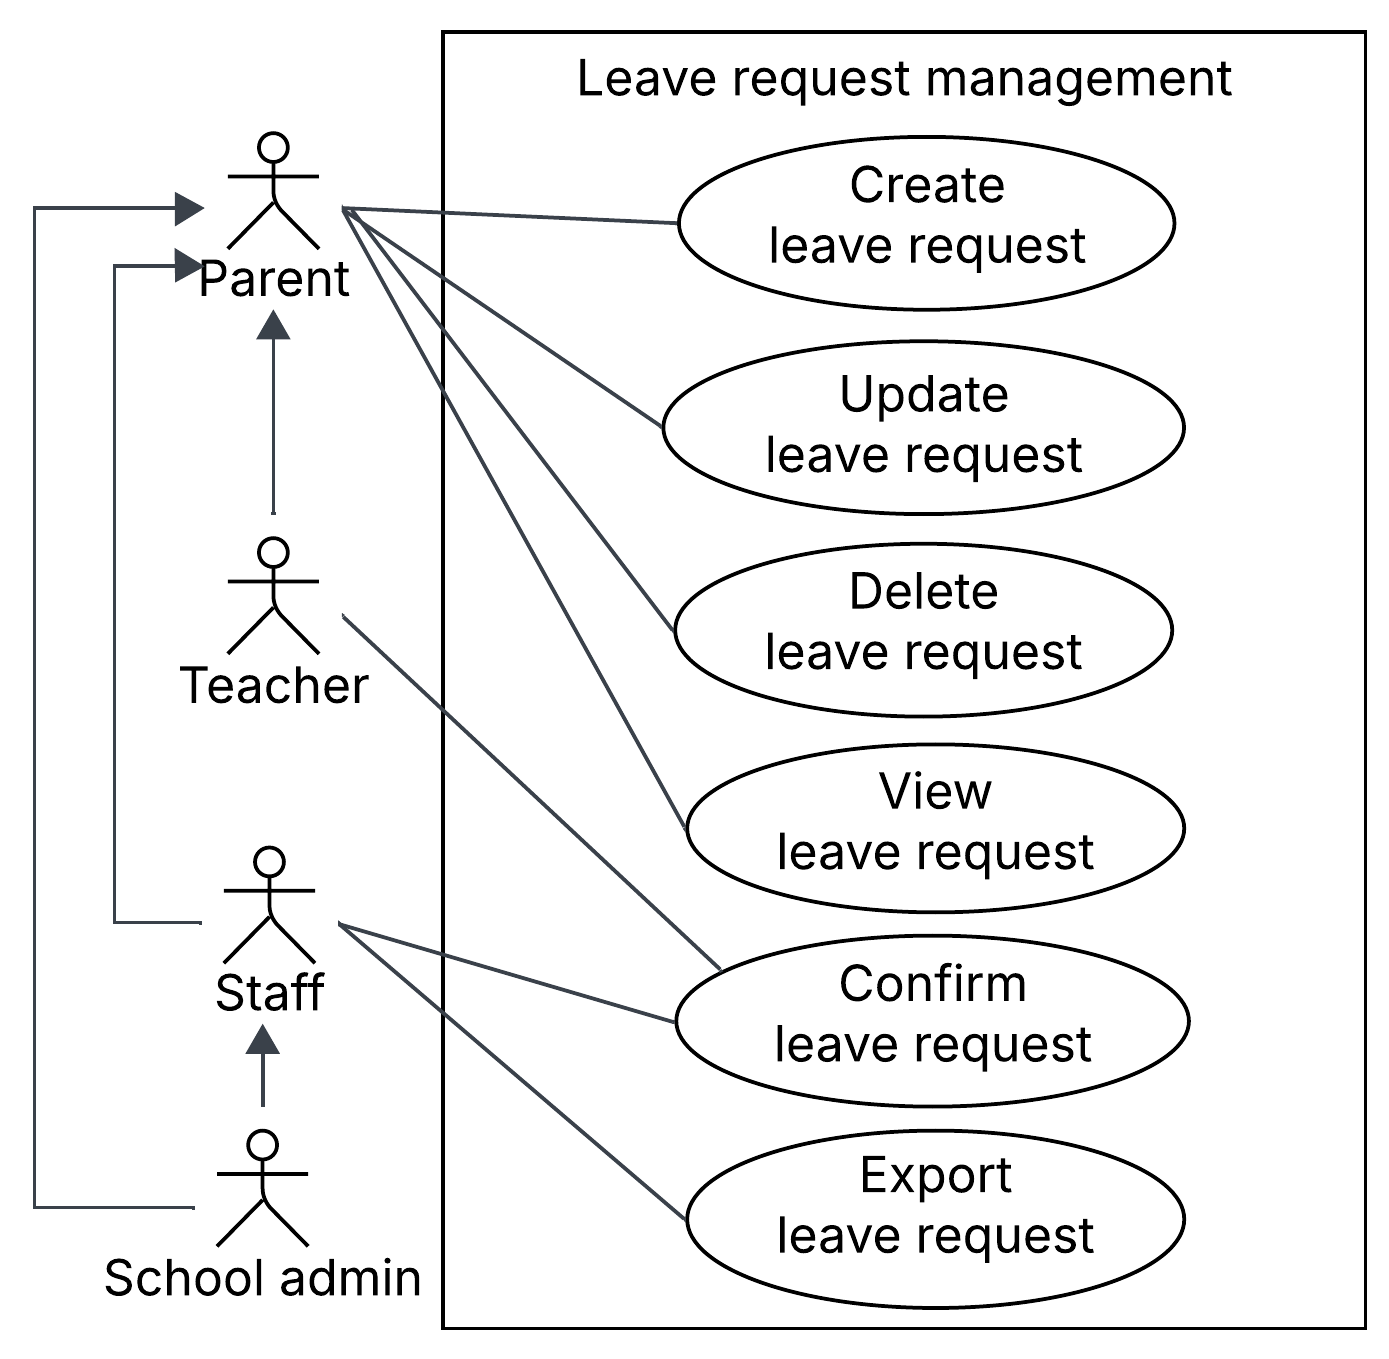
\includegraphics[width=0.55\textwidth]{images/use_case_leave_request_management.png}
%     \caption{Use case diagram for Leave Request Management.}
%     \label{fig:use_case_leave_request_management}
% \end{figure}

% LEAVE REQUEST MANAGEMENT: CREATE STUDENT LEAVE REQUEST
% \renewcommand{\arraystretch}{1.5}
% \begin{longtable}{|>{\raggedright\arraybackslash}p{3.5cm}|
%                   >{\raggedright\arraybackslash}p{10cm}|}
% \caption{Use Case Analysis for the Create Student Leave Request feature.}
% \label{tab:leave_management_student_leave_request} \\
% \endfirsthead
% \endhead
% \hline
%     \textbf{Function name} & \textbf{Create student leave request}\\
%     \hline
%     Actor & Parents \\
%     \hline
%     Description & Support parent create leave requests for their children \\
%     \hline
%     Pre-conditions & {
%         \vspace{-1.7em}
%         \begin{itemize}
%             \item The administrators and teachers must log into the system with valid access rights
%             \vspace{-0.8em}
%             \item The teachers must manage at least one class.
%             \vspace{-1.5em}
%         \end{itemize}    
%     }\\
%     \hline
%     Main flow &  {
%         \vspace{-1.7em}
%         \begin{itemize}
%             \item Teachers selects a class and access the Attendance feature
%             \vspace{-0.8em}
%             \item The system retrieves a list of students with their current status (checked/unchecked).
%             \vspace{-0.8em}
%             \item Teacher selects student and mark attendance status.
%             \vspace{-0.8em}
%             \item System save the records and push notification to parents.
%             \vspace{-0.8em}
%             \item Finish the process of marking student attendance data.
%             \vspace{-1.8em}
%         \end{itemize}    
%     }\\
%     \hline
% \end{longtable}
    


% NEWSFEED MANAGEMENT
% \indent\indent\textbf{2.4.2.4 Newsfeed management Use Case Diagram}
% \vspace{0.5em}
% \par\indent\indent\parbox{0.9\textwidth}{
%     \setlength{\parindent}{2em} 
%     The Newsfeed Management is a communication module that allows teachers to share classroom and school activities through images, videos, and files. Teachers can create, edit, view, comment on, react to, and delete content for the classes they supervise, while parents can only view, comment on, and react to these posts. This feature provides parents with valuable insights into their child's class experiences and improves the connection between home and school.
% }\\
% \begin{figure}[H]
%     \centering
%     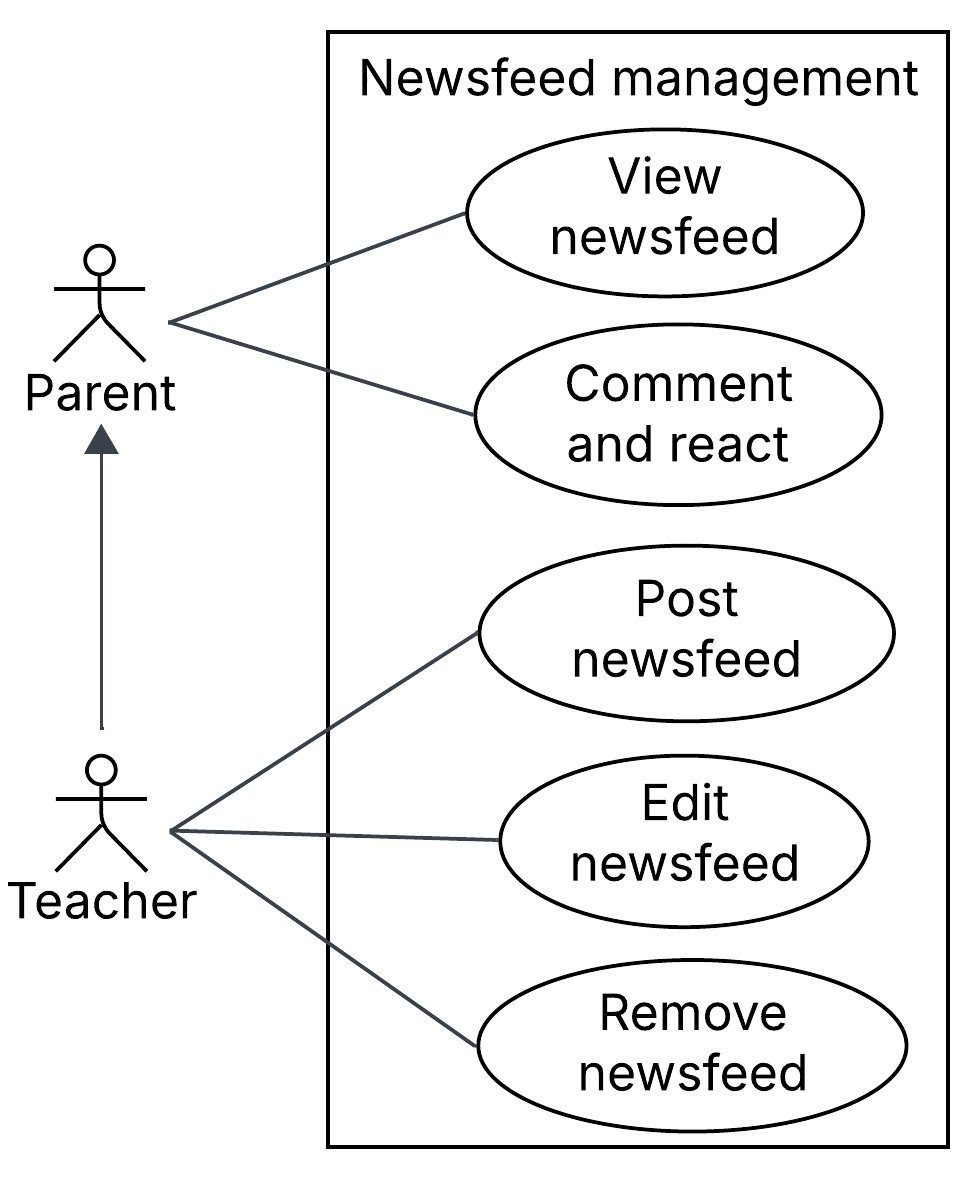
\includegraphics[width=0.5\textwidth]{images/use_case_newsfeed_management.png}
%     \vspace{-0.5em}
%     \caption{Use case diagram for Newsfeed Management.}
%     \label{fig:use_case_newsfeed_management}
% \end{figure}
    

% STUDENT ASSESSMENT MANAGEMENT
% \indent\indent\textbf{2.4.2.5 Student Assessment Management Use Case Diagram}
% \vspace{0.5em}
% \par\indent\indent\parbox{0.9\textwidth}{
%     \setlength{\parindent}{2em} 
%     Student Assessment Management is a module that allows teachers to evaluate individual or multiple students. Teachers can create, modify, and view assessments for the students they supervise, while parents can only view assessments of their children. Additionally, teachers can add supporting files such as images or files for assessment to make it more reliable. This feature helps parent tracks their child's academic progress, achievements, and overall performance in the class.
% }\\
% \begin{figure}[H]
%     \centering
%     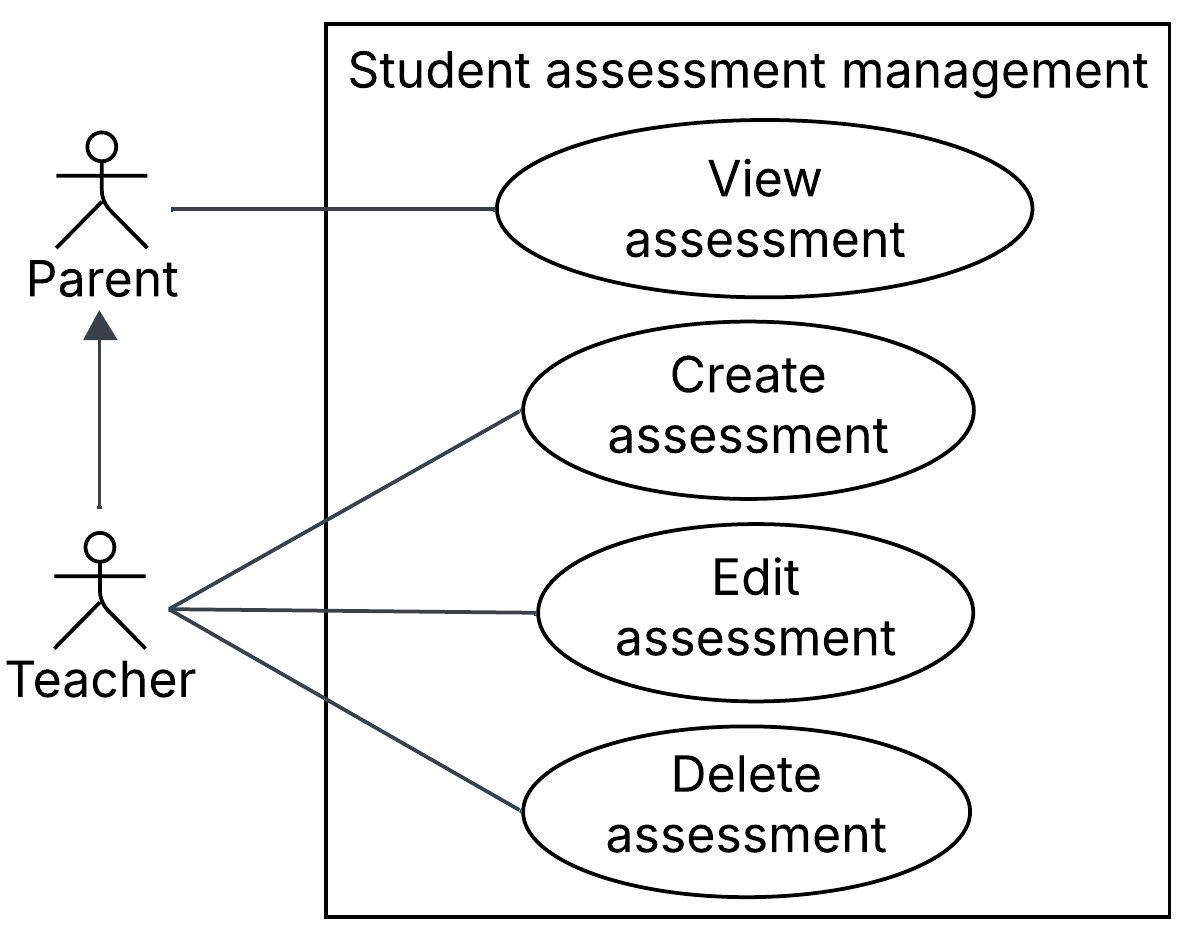
\includegraphics[width=0.6\textwidth]{images/use_case_student_assessment_management.png}
%     \caption{Use case diagram for Student Assessment Management.}
%     \label{fig:use_case_student_assessment_management}
% \end{figure}

% MEDICINE REMINDER MANAGEMENT
% \indent\indent\textbf{2.4.2.6 Medicine Reminder Management Use Case Diagram}
% \vspace{0.5em}
% \par\indent\indent\parbox{0.9\textwidth}{
%     \setlength{\parindent}{2em}
%     Medicine Reminder Management is a module that allows parents to remind teachers to administer medication to their children. Parents can create, modify, delete, and view medicine reminders for their children, while teachers can only view and confirm these reminders. Once a medicine reminder is confirmed by a teacher, parents cannot modify or delete it to ensure accountability and prevent confusion. Additionally, parents can attach images to the reminders to increase reliability. This feature helps ensure proper medication administration while maintaining clear communication between parents and teachers, ultimately supporting children's health and safety in the educational environment.
% }\\
% \begin{figure}[H]
%     \centering
%     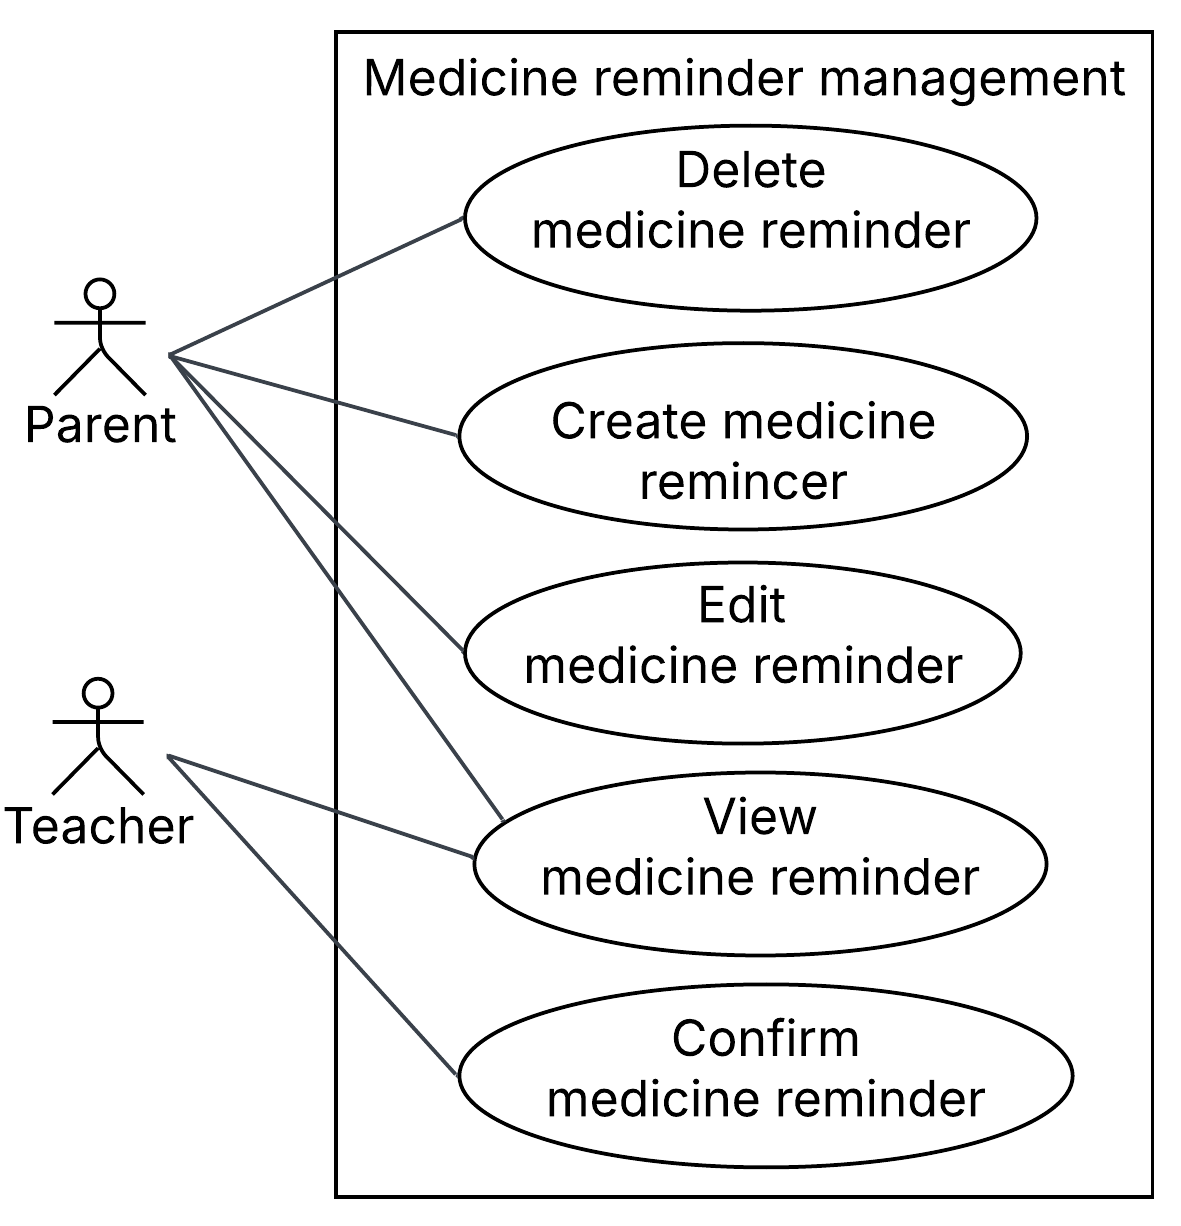
\includegraphics[width=0.55\textwidth]{images/use_case_medicine_reminder.png}
%     \caption{Use case diagram for Medicine Reminder Management.}
%     \label{fig:use_case_medicine_reminder_management}
% \end{figure}

% NOTIFICATION MANAGEMENT
% \indent\indent\textbf{2.4.2.7 Notification Management Use Case Diagram}
% \vspace{0.5em}
% \par\indent\indent\parbox{0.9\textwidth}{
%     \setlength{\parindent}{2em}
%     Notification Management is a module that serves as a communication bridge between schools and parents. School administrators and teachers can create, edit, delete, push, and view notifications, while parents can only receive and read all notifications sent by the school. This feature ensures parents stay informed about important school updates, events, and announcements. The notifications will be pushed to the parent mobile device, and this module eliminates the need for paper notices or phone calls.
% }\\
% \begin{figure}[H]
%     \centering
%     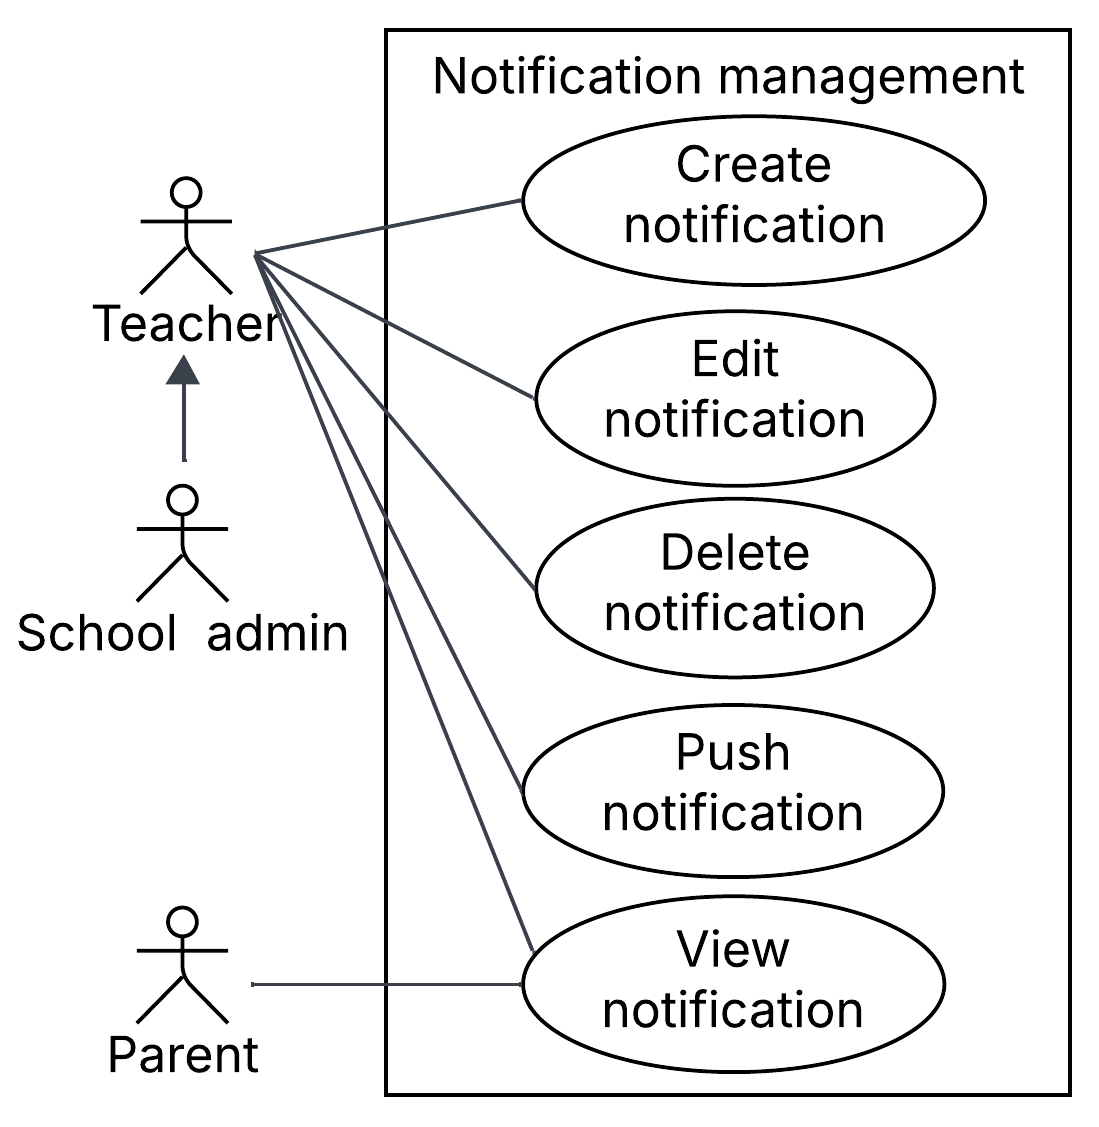
\includegraphics[width=0.55\textwidth]{images/use_case_notification_management.png}
%     \caption{Use Case diagram for Notification Management.}
%     \label{fig:use_case_notification_management}
% \end{figure}

% BUS MANAGEMENT
% \newpage
% \indent\indent\textbf{2.4.2.8 Bus Management Use Case Diagram}
% \vspace{0.5em}
% \par\indent\indent\parbox{0.9\textwidth}{
%     \setlength{\parindent}{2em}
%     Bus Management is a module that manages all aspects related to school transportation services within educational institutions. It enables administrators and staff to efficiently configure, view, and delete bus routes as well as register bus stops for students, ensuring optimized resource allocation and reduced manual time. For parents, the module provides real-time bus tracking and the ability to register designated stops, along with access to bus route information for their children, enhancing transparency and safety.
% }\\
% \begin{figure}[H]
%     \centering
%     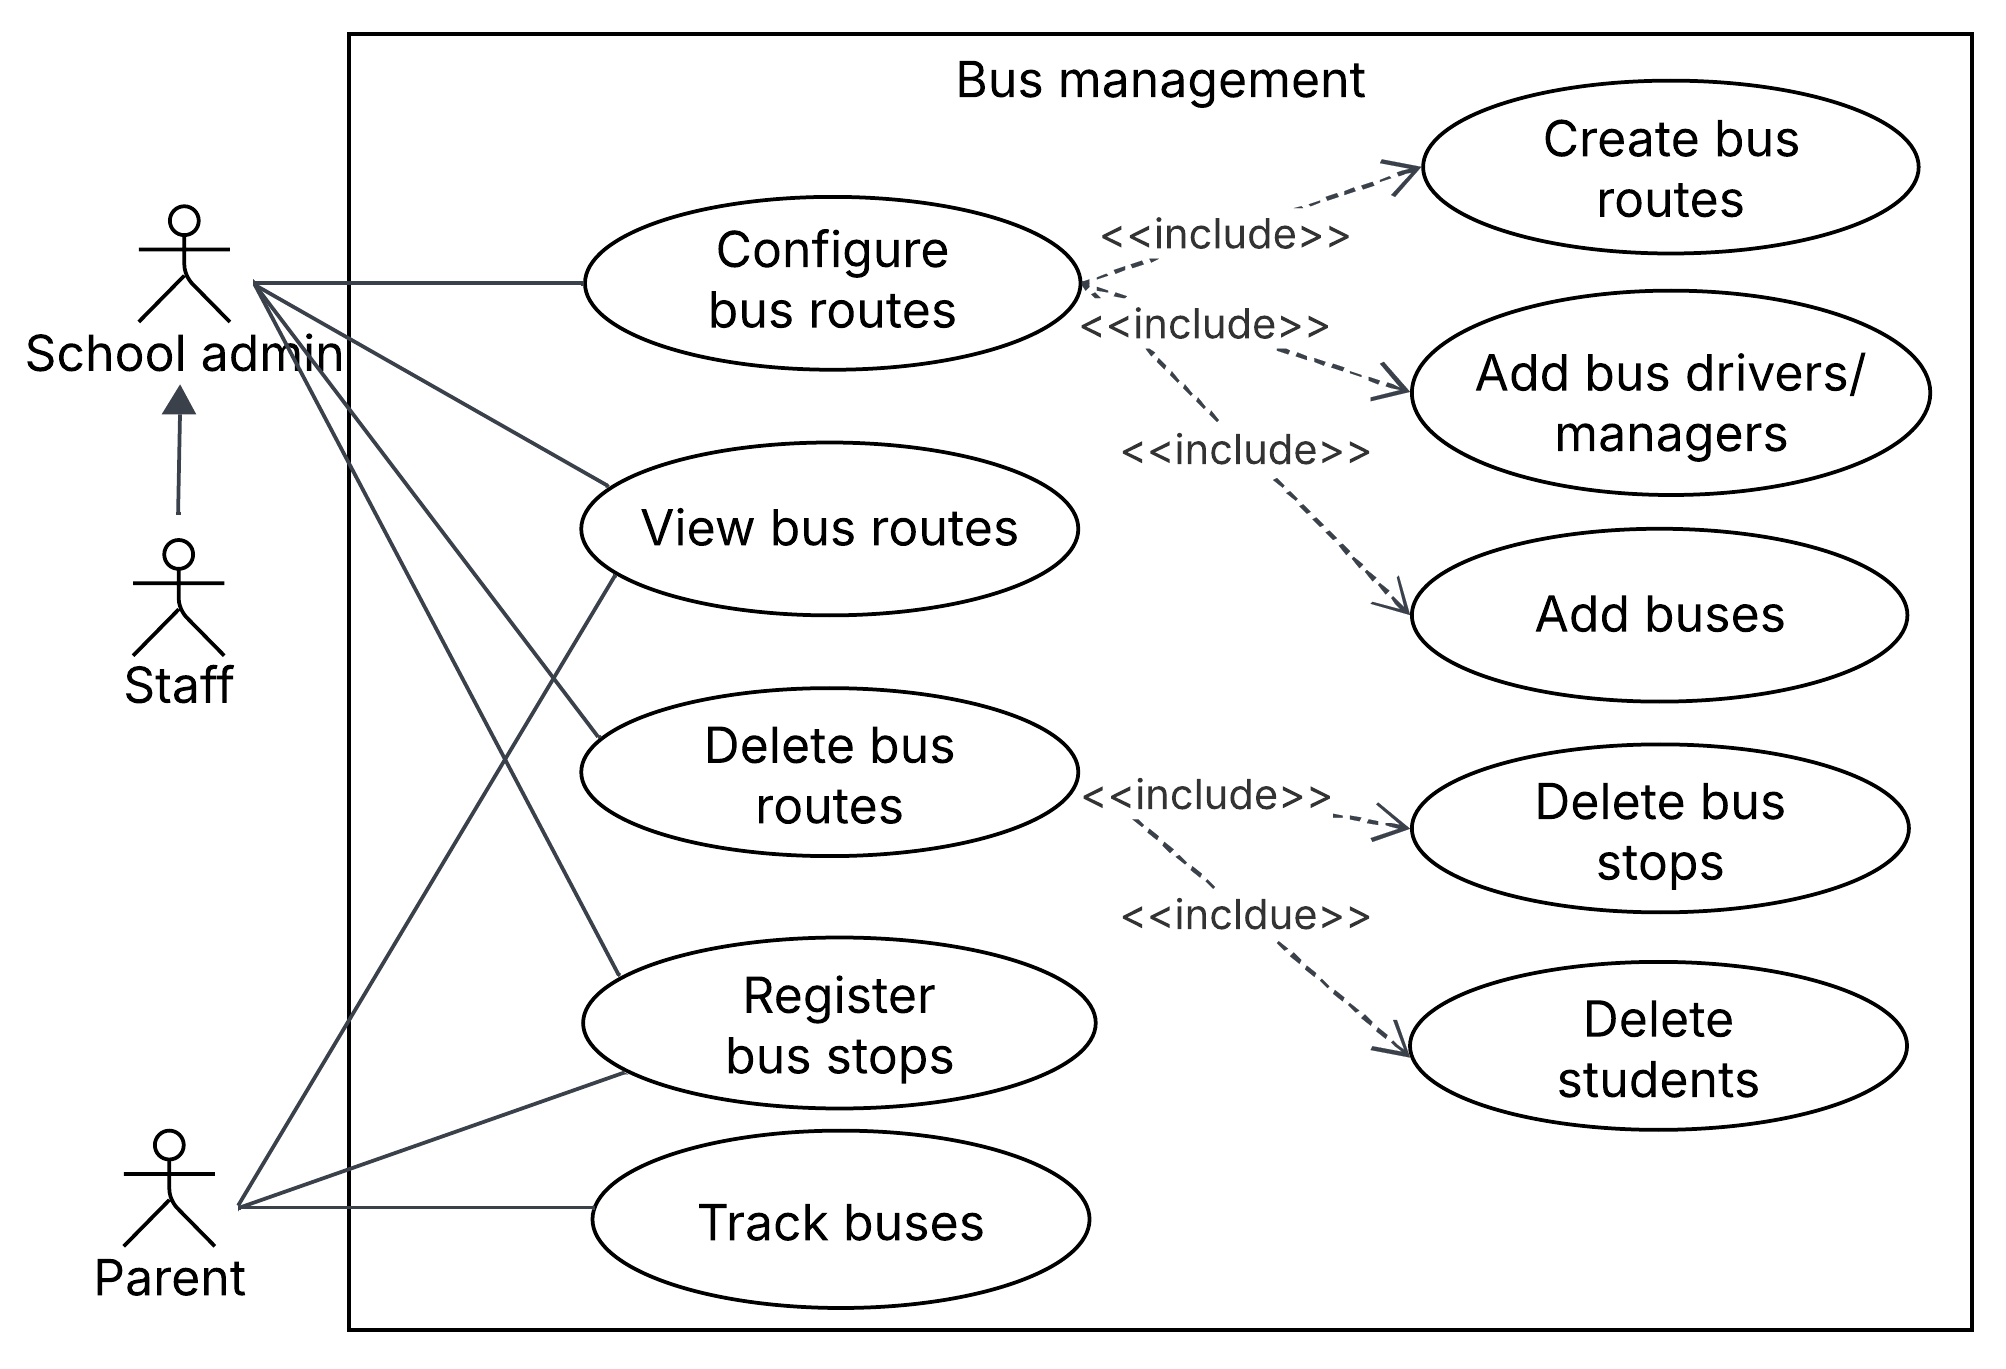
\includegraphics[width=0.9\textwidth]{images/use_case_bus_management.png}
%     \caption{Use Case diagram for Bus Management.}
%     \label{fig:use_case_bus_management}
% \end{figure}


  % 2.5 Use-case specification
  % \subsection{Use case Specification}\label{sec:use_case_specification}
  % \indent

\textbf{This section examines the key features under my responsibility in the GMES School system}, analyzing user role interactions and business logic.
% COMMON
\subsubsection{Common Elements and Flows for All Use Cases}\label{sec:common_usecase}
\par\indent\indent\parbox{0.9\textwidth}{
    This section establishes the foundational elements that are consistent across all use cases documented in \textbf{\autoref{sec:use_case_specification} \nameref{sec:use_case_specification}}
}\\[0.25cm]
\indent\textbf{2.4.1.1 Standard Pre-conditions}\\
\indent\indent User must be logged into the system with valid credentials.\\
\indent\indent User must have appropriate role-based permissions for the specific function.\\[0.2cm]
\indent\textbf{2.4.1.2 Standard Request Data}\\
\indent\indent User session data (token, context).\\[0.2cm]
\indent\textbf{2.4.1.3 Standard Alternative Flow}
\vspace{0.2cm}
\par\indent\indent\parbox{0.9\textwidth}{\textbf{Network/server error}: If network/server errors occur, the system displays an alert about connectivity issues, notifying users when features are unavailable. This allows users to retry or report the problem to support staff.}

% IMPORT EMPLOYEE DATA
\subsubsection{Personnel Management: Import Employee Data}
\indent\indent\textbf{2.4.2.1 Brief description}
\vspace{0.5em}
\par\indent\indent\parbox{0.9\textwidth}{
    This use case demonstrates how school administrators and staff import employee information using Excel files through the system's web application.
}\\

\vspace{0.5em}
\indent\textbf{2.4.2.2 Flow of event}
\vspace{0.5em}
\par\indent\indent\textbf{A. Basic flow}
\vspace{-0.5em}
\renewcommand{\arraystretch}{1.5}
\begin{longtable}{|>{\raggedright\arraybackslash}p{4.5cm}|
                  >{\raggedright\arraybackslash}p{6cm}|
                  >{\raggedright\arraybackslash}p{4.5cm}|}                  
\caption{Import employee data via Excel basic flow.}
\label{tab:employee_management_basic_flow1} \\
\hline
\centering\textbf{User action} & \centering\textbf{System action} & \centering\arraybackslash\textbf{Data} \\
\hline
\endfirsthead
\endhead

1. User navigates to the Employee profiles tab. & 2. The system retrieves the organizations that are managed by the user.& \\
    \hline
    3. User selects a department and clicks the "Upload employee file" button. &4. System prepares to receive the Excel file.&\\
    \hline
    5. User uploads the Excel file.& 6. System validates the file format and checks for required columns.
    &\par{Request:
        \vspace{-0.8em}
        \begin{itemize}
            \item Excel file
        \end{itemize}
    } \\
    \hline
    &7. The system reads the file and checks each employee code to determine whether the employee is new or existing.&\\
    \hline
    &8. System verifies all data fields in each row.&\\
    \hline
    &9. If the employee is new, the system adds a new record to the database, otherwise, the system updates the existing employee information.&\\
    \hline
    &10. The system reloads and displays the latest employee list for the chosen department.&\\
    \hline
\end{longtable}

\par\indent\indent\textbf{B. Alternative flow}
\vspace{-0.5em}
\renewcommand{\arraystretch}{1.5}
\begin{longtable}{|>{\raggedright\arraybackslash}p{4.5cm}|
                  >{\raggedright\arraybackslash}p{6cm}|
                  >{\raggedright\arraybackslash}p{4.5cm}|}                  
\caption{Import employee data via Excel alternative flow.}
\label{tab:employee_management_import_data_alternative_flow} \\
\hline
\centering\textbf{User action} & \centering\textbf{System action} & \centering\arraybackslash\textbf{Data} \\
\hline
\endfirsthead
\endhead

5. User uploads the Excel file.& 6a. System detects invalid file format (not .xlsx/.xls).
&\par{Request:
    \vspace{-0.8em}
    \begin{itemize}
        \item Excel file
        \vspace{-1.4em}
    \end{itemize}
}\\

\hline
&6b. The system checks for missing required fields such as employee code, name, ID number, work office, etc.&
\par{Request:
    \vspace{-0.8em}
    \begin{itemize}
        \item Excel file
    \end{itemize}
}\\
\hline
&6c. For valid file, system detects a duplication in ID number.&\\
\hline
&6d. System identifies invalid data in a row such as wrong date format.& \\
\hline
&6e. System detects reference data mismatch such as invalid department code.&\\
\hline
&7. The system updates the valid data that it read before encountering the error, the rest of the file will be ignored. &\\
\hline
&10. The system displays an error message.&\\
\hline
\end{longtable}
\newpage
\indent\textbf{2.4.2.3 Notes}\\
\vspace{-0.7em}
\par\indent\indent\parbox{0.9\textwidth}{
    The uploaded Excel file must follow the system's predefined template. User can download the template from the web application of the system.
}\\[0.2cm]
\indent\textbf{2.4.2.4 Pre-conditions}\\
\indent\indent The uploaded file must be Excel file (.xlsx/.xls).\\[0.2cm]
\indent\textbf{2.4.2.5 Post-conditions}\\
\vspace{-0.7em}
\par\indent\indent\parbox{0.9\textwidth}{
    On success, the system updates all employee data from the file to the database and refreshes the data. If an error occurs, the system updates only the valid data before it encounters the error and displays an error message.
}\\

% STUDENT ATTENDANCE MANAGEMENT
\subsubsection{Attendance Management: Mark Student Attendance}
\indent\indent\textbf{2.4.3.1 Brief description}
\vspace{0.5em}
\par\indent\indent\parbox{0.9\textwidth}{
    This use case demonstrates how teacher and bus managers mark student attendance through the mobile app, and how the system handles the request.
}\\

\vspace{0.5em}
\indent\textbf{2.4.3.2 Flow of event}
\vspace{0.5em}
\par\indent\indent\textbf{A. Basic flow}
\vspace{1em}
\par\indent\indent\indent\parbox{0.87\textwidth}{\textbf{Mark student attendance in class}: This feature enables teachers to record student attendance when they in class.}
\vspace{-1em}
\renewcommand{\arraystretch}{1.5}
\begin{longtable}{|>{\raggedright\arraybackslash}p{4.5cm}|
                  >{\raggedright\arraybackslash}p{6cm}|
                  >{\raggedright\arraybackslash}p{4.5cm}|}                  
\caption{Mark student attendance basic flow.}
\label{tab:student_attendance_mark_presence_class_basic_flow}\\
\hline
\centering\textbf{User action} & \centering\textbf{System action} & \centering\arraybackslash\textbf{Data} \\
\hline
\endfirsthead
\endhead

1. User selects a class and navigates to Attendance function. & 2. The system retrieves and display a list of students with their current status (checked/unchecked).& 
    \par{Request:
        \vspace{-0.8em}
        \begin{itemize}
            \item Id of the selected class
        \end{itemize}
    } 
    \vspace{-0.8em}
    \par{Response: 
        \vspace{-0.8em}
        \begin{itemize}
            \item A list of student.
            \vspace{-1.5em}
        \end{itemize}
    }\\
\hline
3. User selects students and marks their attendance status.&4. System processes the request and sends the attendance data to the timesheet service to update records for selected students.&
\par{Request: 
        \vspace{-0.8em}
        \begin{itemize}
            \item List of selected students.
            \vspace{-0.8em}
            \item Attendance status.
            \vspace{-2.5em}
        \end{itemize}
    }\\
\hline
&5. System pushes an attendance notification to parents' phones and saves it to the database.&\\
\hline
&6. System reloads the list of student and diplay to user.&\\
\hline
\end{longtable}

\par\indent\indent\indent\parbox{0.87\textwidth}{\textbf{Mark student presence on buses}: Similar to classroom attendance, but it has several key differences. This features enables 
transportation staff record student presence at bus stops with automatic geolocation capture.}
\vspace{0.5em}
\newpage
\par\indent\indent\textbf{B. Alternative flow}
\vspace{-0.5em}
\renewcommand{\arraystretch}{1.5}
\begin{longtable}{|>{\raggedright\arraybackslash}p{4.5cm}|
                  >{\raggedright\arraybackslash}p{6cm}|
                  >{\raggedright\arraybackslash}p{4.5cm}|}                  
\caption{Mark student presence alternative flow: Mark attendance in the past.}
\label{tab:student_attendance_past_date_alternative_flow} \\
\hline
\centering\textbf{User action} & \centering\textbf{System action} & \centering\arraybackslash\textbf{Data} \\
\hline
\endfirsthead
\endhead
1. User selects a day in the past.& 2. System prevents user from selecting students to mark presence in the past.&\\
\hline
\end{longtable}
\vspace{-0.5cm}
\renewcommand{\arraystretch}{1.5}
\begin{longtable}{|>{\raggedright\arraybackslash}p{4.5cm}|
                  >{\raggedright\arraybackslash}p{6cm}|
                  >{\raggedright\arraybackslash}p{4.5cm}|}                  
\caption{Mark student presence alternative flow: Mark attendance in future date}
\label{tab:student_attendance_future_date_alternative_flow} \\
\hline
\centering\textbf{User action} & \centering\textbf{System action} & \centering\arraybackslash\textbf{Data} \\
\hline
\endfirsthead
\endhead
1. User selects the calendar.& 2. System displays a calendar with disable future date to prevent marking attendance for future date.&\\
\hline
\end{longtable}
\vspace{-0.5cm}
\renewcommand{\arraystretch}{1.5}
\begin{longtable}{|>{\raggedright\arraybackslash}p{4.5cm}|
                  >{\raggedright\arraybackslash}p{6cm}|
                  >{\raggedright\arraybackslash}p{4.5cm}|}                  
\caption{Mark student presence alternative flow: Contact parent.}
\label{tab:student_attendance_contact_parent_alternative_flow} \\
\hline
\centering\textbf{User action} & \centering\textbf{System action} & \centering\arraybackslash\textbf{Data} \\
\hline
\endfirsthead
\endhead
1. User selects the call parents option.& 2. System retrieves the parent contact information of the selected student.&\\
\hline
&3. If parent contact information exists, the system initiates a call to their mobile number, else it displays an error message.&\\
\hline
\end{longtable}

\indent\textbf{2.4.3.3 Notes}\\
\indent\indent There is no note.
\vspace{0.5em}

\indent\textbf{2.4.3.4 Pre-conditions}\\
\indent\indent The student must be either in the class or registered to a bus stop.

\vspace{0.5em}
\indent\textbf{2.4.3.5 Post-conditions}\\
\vspace{-0.7em}
\par\indent\indent\parbox{0.87\textwidth}{
    On success, the system updates student attendance records into the database and notifies parents via their mobile phones. Otherwise, it returns an error message without making any updates.
}\\

% STUDENT ATTENDANCE MANAGEMENT: GENERATE STUDENT ATTENDANCE REPORT
\subsubsection{Attendance Management: Generate Student Attendance Report}
\indent\indent\textbf{2.4.4.1 Brief description}
\vspace{0.5em}
\par\indent\indent\parbox{0.9\textwidth}{
    This use case demonstrates how administrators, authorized staff, and teachers generate a student attendance report through the system's web app, and how the system processes the request.
}\\

\vspace{0.5em}
\indent\textbf{2.4.4.2 Flow of event}
\vspace{0.5em}
\par\indent\indent\textbf{A. Basic flow}
\vspace{-0.5em}
\renewcommand{\arraystretch}{1.5}
\begin{longtable}{|>{\raggedright\arraybackslash}p{4.5cm}|
                  >{\raggedright\arraybackslash}p{6cm}|
                  >{\raggedright\arraybackslash}p{4.5cm}|}                  
\caption{View student attendance record for teacher or bus manager basic flow.}
\label{tab:student_attendance_view_attendance_basic_flow}\\
\hline
\centering\textbf{User action} & \centering\textbf{System action} & \centering\arraybackslash\textbf{Data} \\
\hline
\endfirsthead
\endhead
1. User navigates to "Student Attendance Report" function. & 2. The system retrieves the
departments which are managed by the user.& 
    \par{Response: 
        \vspace{-0.8em}
        \begin{itemize}
            \item A list of departments.
            \vspace{-1.2em}
        \end{itemize}
    }\\
\hline
3. User selects a department and select the date range.&4. System processes the request and sends the data to timesheet service.&
\par{Request: 
        \vspace{-0.8em}
        \begin{itemize}
            \item Id of the class
            \vspace{-0.8em}
            \item Selected period
            \vspace{-1.5em}
        \end{itemize}
    }\\
\hline
&5. The timesheet service fetches attendance data, then maps each student's attendance status to every date in the selected period.&
\par{Response: 
        \vspace{-0.8em}
        \begin{itemize}
            \item Student attendance records.
            \vspace{-1.5em}
        \end{itemize}
    }\\
\hline
&6. The process completes and displays the data to the user.&\\
\hline
\end{longtable}
\par\indent\indent\textbf{B. Alternative flow}
\begin{adjustwidth}{4.5em}{0em}
    Follow the Standard Alternative Flow in \textbf{\autoref{sec:common_usecase} \nameref{sec:common_usecase}}
\end{adjustwidth}
% \begin{adjustwidth}{4.5em}{0em}
%     \textbf{No attendance records found}: When a user navigates to the attendance function and no attendance records are available, the system responds differently based on the user's role. If the user is a teacher or bus manager, the system displays a list of students in their assigned class or bus route, but shows these students with no attendance status recorded. This allows educational staff to see which students are enrolled but haven't had their attendance marked yet. Alternatively, if the user is a parent accessing the system, the system displays a message box indicating that no attendance records are currently available for their child, providing clear communication about the absence of attendance data without showing unnecessary student lists.
% \end{adjustwidth}

\vspace{0.5em}
\indent\textbf{2.4.4.3 Notes}\\
\indent\indent There is no note.
\vspace{0.5em}

\indent\textbf{2.4.4.4 Pre-conditions}\\
\indent\indent The user must be assigned to at least one class.
\vspace{0.5em}

\indent\textbf{2.4.4.5 Post-conditions}\\
\vspace{-0.7em}
\par\indent\indent\parbox{0.9\textwidth}{
    If the use case is successful, student attendance records are retrieved and displayed to the user. Otherwise, the system displays an error message.
}\\
% LEAVE REQUEST MANAGEMENT: CREATE LEAVE REQUEST
\subsubsection{Leave Request Management: Create Leave Requests}
\indent\indent\textbf{2.4.5.1 Brief description}
\vspace{0.5em}
\par\indent\indent\parbox{0.9\textwidth}{
    This use case describes how leave requests can be created via mobile app (by parents/teachers) and how the system processes the submitted requests.
}\\

\vspace{0.5em}
\indent\textbf{2.4.5.2 Flow of event}
\vspace{0.5em}
\par\indent\indent\textbf{A. Basic flow}
\vspace{-0.5em}
\renewcommand{\arraystretch}{1.5}
\begin{longtable}{|>{\raggedright\arraybackslash}p{4.5cm}|
                  >{\raggedright\arraybackslash}p{6cm}|
                  >{\raggedright\arraybackslash}p{4.5cm}|}                  
\caption{Create leave request on web application.}
\label{tab:leave_request_management_create_on_web_basic_flow}\\
\hline
\centering\textbf{User action} & \centering\textbf{System action} & \centering\arraybackslash\textbf{Data} \\
\hline
\endfirsthead
\endhead

1. User opens 'Leave Request' and clicks 'Create'. & 2. The system displays create leave request screen. &\\ 
\hline
& 3. System retrieves absence types.& 
    \par{Response:
        \vspace{-0.8em}
        \begin{itemize}
            \item Absence types
            \vspace{-1.2em}
        \end{itemize}
    } \\
\hline
4. User fills all the required fields and clicks the "Save" button.&5. System processes the request and validate the leave requests (e.g., check for overlapping leave request, valid date range, maximum absence days, holiday conflicts).&
\par{Request: 
        \vspace{-0.8em}
        \begin{itemize}
            \item Leave request.
        \end{itemize}
    }\\
\hline
&6. If the leave request is valid, the system saves it to database.&\\
\hline
&7. System resfreshes the list of leave requests and displays to user.&
\par{Response: 
        \vspace{-0.8em}
        \begin{itemize}
            \item Leave requests.
        \end{itemize}
    }\\
\hline
\end{longtable}

\par\indent\indent\textbf{B. Alternative flow}
\vspace{0.3cm}
\par\indent\indent\indent\parbox{0.9\textwidth}{\textbf{Required fields missing}: When a user creates a leave request but does not provide all required fields, the system disables the Save button, preventing the user from submitting an incomplete request. It ensures all necessary information is provided and maintains data integrity.}
\vspace{0.05cm}
\par\indent\indent\indent\parbox{0.9\textwidth}{\textbf{Invalid leave request}:}
\vspace{-2em}
\renewcommand{\arraystretch}{1.5}
\begin{longtable}{|>{\raggedright\arraybackslash}p{4.5cm}|
                  >{\raggedright\arraybackslash}p{6cm}|
                  >{\raggedright\arraybackslash}p{4.5cm}|}                  
\caption{Create leave requests alternative flow: Invalid leave request.}
\label{tab:leave_request_management_invalid_alternative_flow} \\
\hline
\centering\textbf{User action} & \centering\textbf{System action} & \centering\arraybackslash\textbf{Data} \\
\hline
\endfirsthead
\endhead
5. User fills all required fields and taps "Save" button.& 6. System receives the leave request and validates it.&\\
\hline
& 6a. If validation fails (overlapping requests, exceeds remaining/maximum days, holiday conflicts, or payroll cycle issues), system returns error message.&
\par{Request: 
        \vspace{-0.8em}
        \begin{itemize}
            \item Bad request message.
        \end{itemize}
    }
\\
\hline
\end{longtable}

\indent\textbf{2.4.5.3 Notes}\\
\indent\indent There is no note.
\vspace{0.5em}

\indent\textbf{2.4.5.4 Pre-conditions}\\
\indent\indent Follow the Standard Pre-conditions in \textbf{\autoref{sec:common_usecase}}
\vspace{0.5em}

\indent\textbf{2.4.5.5 Post-conditions}\\
\vspace{-0.7em}
\par\indent\indent\parbox{0.9\textwidth}{
    If the use case is successful, the system saves the leave request to the database and notifies teachers via their mobile phones. Otherwise, the system displays an error message without creating the request.
}\\

% LEAVE REQUEST MANAGEMENT: CONFIRM LEAVE REQUEST
\subsubsection{Leave Request Management: Confirm Leave Requests}
\indent\indent\textbf{2.4.6.1 Brief description}
\vspace{0.5em}
\par\indent\indent\parbox{0.9\textwidth}{
    This use case shows teachers approve, reject, or revoke leave requests for students through the mobile applications.
}\\

\vspace{0.5em}
\indent\textbf{2.4.6.2 Flow of event}
\vspace{0.5em}
\par\indent\indent\textbf{A. Basic flow}
\vspace{-0.5em}
\renewcommand{\arraystretch}{1.5}
\begin{longtable}{|>{\raggedright\arraybackslash}p{4.5cm}|
                  >{\raggedright\arraybackslash}p{6cm}|
                  >{\raggedright\arraybackslash}p{4.5cm}|}                  
\caption{Confirm leave request on mobile application.}
\label{tab:leave_request_management_confirm_request_on_mobile_basic_flow}\\
\hline
\centering\textbf{User action} & \centering\textbf{System action} & \centering\arraybackslash\textbf{Data} \\
\hline
\endfirsthead
\endhead

1. User navigates to "Approve Leave request" function. & 2. The system retrieves a list of leave request of students which are managed by the user.&
    \par{Response:
        \vspace{-0.8em}
        \begin{itemize}
            \item List of leave request
            \vspace{-1.5em}
        \end{itemize}
    } \\
\hline
&3. System retrieves the leaves request displays to user in 3 seperated groups: pending, approved and declined.& \\
\hline
4. User approves, rejectes, or revokes a leave request.&5. System updates the leave request status.&
\par{Request: 
        \vspace{-0.8em}
        \begin{itemize}
            \item Selected leave request.
            \vspace{-1.2em}
        \end{itemize}
    }\\
\hline
&6. System resfreshes the list of leave requests and displays the updated list to user.&
\par{Response: 
        \vspace{-0.8em}
        \begin{itemize}
            \item List of updated leave request.
            \vspace{-1.2em}
        \end{itemize}
    }\\
\hline
\end{longtable}

\par\indent\indent\textbf{B. Alternative flow}
\begin{adjustwidth}{4.5em}{0em}
    Follow the Standard Alternative Flow in \textbf{\autoref{sec:common_usecase} \nameref{sec:common_usecase}}
\end{adjustwidth}
\vspace{0.5em}

\indent\textbf{2.4.6.3 Notes}\\
\indent\indent There is no note.
\vspace{0.5em}

\indent\textbf{2.4.6.4 Pre-conditions}\\
\indent\indent Follow the Standard Pre-conditions in \textbf{\autoref{sec:common_usecase}}

\vspace{0.5em}
\indent\textbf{2.4.6.5 Post-conditions}\\
\vspace{-0.7em}
\par\indent\indent\parbox{0.9\textwidth}{
    On success, the system updates the leave request status in the database and notifies parents via mobile phones (for student requests). Otherwise, the system displays an error message without any updates.
}\\


% NEWSFEED MANAGEMENT: POST NEWSFEED
\subsubsection{Newsfeed Management: Post Newsfeed}
\indent\indent\textbf{2.4.7.1 Brief description}
\vspace{0.5em}
\par\indent\indent\parbox{0.9\textwidth}{
   This use case shows how teachers create posts with images, videos, and files via the system's mobile application and how the system processes them.
}\\
\newpage
\indent\textbf{2.4.7.2 Flow of event}
\vspace{0.5em}
\par\indent\indent\textbf{A. Basic flow}
\vspace{-0.5em}
\renewcommand{\arraystretch}{1.5}
\begin{longtable}{|>{\raggedright\arraybackslash}p{4.5cm}|
                  >{\raggedright\arraybackslash}p{6cm}|
                  >{\raggedright\arraybackslash}p{4.5cm}|}                  
\caption{Post newsfeed basic flow.}
\label{tab:newsfeed_management_post_newsfeed_basic_flow}\\
\hline
\centering\textbf{User action} & \centering\textbf{System action} & \centering\arraybackslash\textbf{Data} \\
\hline
\endfirsthead
\endhead

1. User selects a class and taps "Add" button. & 2. The system displays the post creation screen.& \\
\hline
3. User writes post content, adds attachments, and taps the "Post" button. & 4. System receives the POST request from the user and validates the attachment size of the post.& 
\par{Request:
        \vspace{-0.8em}
        \begin{itemize}
            \item Post content
            \vspace{-0.8em}
            \item List of attachment in Base64 format
            \vspace{-1.5em}
        \end{itemize}
    }\\
\hline
&5. The system saves the post content to database and attachments to server.&\\
\hline
&6. System refreshes the newsfeed list (page 0, size 10).&
\par{Request: 
        \vspace{-0.8em}
        \begin{itemize}
            \item Page number, size
        \end{itemize}
    }
\vspace{-0.8em}
\par{Response: 
    \vspace{-0.8em}
    \begin{itemize}
        \item Newsfeed posts.
        \vspace{-1.5em}
    \end{itemize}
}\\
\hline
\end{longtable}

\par\indent\indent\textbf{B. Alternative flow}
\vspace{-0.5em}
\renewcommand{\arraystretch}{1.5}
\begin{longtable}{|>{\raggedright\arraybackslash}p{4.5cm}|
                  >{\raggedright\arraybackslash}p{6cm}|
                  >{\raggedright\arraybackslash}p{4.5cm}|}                  
\caption{Post newsfeed alternative flow.}
\label{tab:newsfeed_management_post_newsfeed_alternative_flow}\\
\hline
\centering\textbf{User action} & \centering\textbf{System action} & \centering\arraybackslash\textbf{Data} \\
\hline
\endfirsthead
\endhead
&5. System rejects post because the total attachments exceed 100MB, and return a bad request message.&
\par{Response:
        \vspace{-0.8em}
        \begin{itemize}
            \item Bad request message
            \vspace{-1.5em}
        \end{itemize}
    }\\
\hline
6. User removes or reduces the oversized attachment and retries.& 7. System process and validate newsfeed post (similar to steps 4 - 6 in the \textbf{Post newsfeed basic flow}).&\\
\hline
\end{longtable}

\indent\textbf{2.4.7.3 Notes}\\
\indent\indent There is no note.
\vspace{0.5em}

\indent\textbf{2.4.7.4 Pre-conditions}\\
\indent\indent The total attachment size must below or equal to 100 MB.
\vspace{0.5em}

\indent\textbf{2.4.7.5 Post-conditions}\\
\vspace{-0.7em}
\par\indent\indent\parbox{0.9\textwidth}{
    If the use case is successful, the system saves newsfeed post to database and server, making it visible in the newsfeed of the class. Otherwise, the system displays an error message and no creation is performed.
}\\

% MEDICINE REMINDER MANAGEMENT: CONFIRM MEDICINE REMINDER
\subsubsection{Medicine reminder management: Confirm medicine reminder}
\indent\indent\textbf{2.4.8.1 Brief description}
\vspace{0.5em}
\par\indent\indent\parbox{0.9\textwidth}{
    This use case describes how teachers confirm medicine reminders for students through the mobile application and how the system processes the confirmation.
}\\

\vspace{0.5em}
\indent\textbf{2.4.8.2 Flow of event}
\vspace{0.5em}
\par\indent\indent\textbf{A. Basic flow}
\vspace{-0.5em}
\renewcommand{\arraystretch}{1.5}
\begin{longtable}{|>{\raggedright\arraybackslash}p{4.5cm}|
                  >{\raggedright\arraybackslash}p{6cm}|
                  >{\raggedright\arraybackslash}p{4.5cm}|}                  
\caption{Confirm medicine reminder basic flow.}
\label{tab:medicine_reminder_management_confirm_basic_flow}\\
\hline
\centering\textbf{User action} & \centering\textbf{System action} & \centering\arraybackslash\textbf{Data} \\
\hline
\endfirsthead
\endhead

1. User selects a medicine reminder to confirm.&2. The system retrieves and displays the detailed of the selected medicine reminder.&
\par{Request:
        \vspace{-0.8em}
        \begin{itemize}
            \item Reminder ID
            \vspace{-0.8em}
        \end{itemize}
    }
    \par{Response:
        \vspace{-0.8em}
        \begin{itemize}
            \item Medicine reminder details
            \vspace{-1.5em}
        \end{itemize}
    }\\
\hline
3. User selects medicines received from parents, adds a confirmation note, and confirms the reminder.&4. System updates the medicine reminder status and saves the confirming user's information.&
\par{Request:
        \vspace{-0.8em}
        \begin{itemize}
            \item Reminder ID
            \vspace{-0.8em}
            \item Confirmation note
            \vspace{-0.8em}
            \item Received medicine items
            \vspace{-1.5em}
        \end{itemize}
    }\\
\hline
& 5. The system pushes a confirmation notification to parents.&\\
\hline
\end{longtable}

\par\indent\indent\textbf{B. Alternative flow}
\vspace{-0.5em}
\renewcommand{\arraystretch}{1.5}
\begin{longtable}{|>{\raggedright\arraybackslash}p{4.5cm}|
                  >{\raggedright\arraybackslash}p{6cm}|
                  >{\raggedright\arraybackslash}p{4.5cm}|}                  
\caption{Confirm medicine reminder alternative flow.}
\label{tab:medicine_reminder_management_alternative_flow}\\
\hline
\centering\textbf{User action} & \centering\textbf{System action} & \centering\arraybackslash\textbf{Data} \\
\hline
\endfirsthead
\endhead
1. User selects a medicine reminder to confirm.&2a. System validates the confirmation date against with the usage date of the reminder.&\\
\hline
&2b. If the confirmation date is after the medicine's usage date, the system blocks the confirmation and displays an error message.&\\
\hline
\end{longtable}

\indent\textbf{2.4.8.3 Notes}
\par\indent\indent\parbox{0.9\textwidth}{
    Once confirmed, the medicine reminder status cannot be reverted to pending.
}
\vspace{0.5em}

\indent\textbf{2.4.8.4 Pre-conditions}\\
\indent\indent  Teachers must be assigned at lease one class.
\vspace{0.25em}
\par\indent\indent\parbox{0.9\textwidth}{
    The confirmation date must not be after the medicine usage date.
}
\vspace{0.5em}

\indent\textbf{2.4.8.5 Post-conditions}\\
\vspace{-0.7em}
\par\indent\indent\parbox{0.9\textwidth}{
    If the use case is successful, the system updates the medicine reminder status, and saves information of the confirmation user. In case of failure, the system displays an error message and no updation is performed.
}\\

% NOTIFICATION MANAGEMENT: PUSH NOTIFICATION
\subsubsection{Notification management: Push notification}
\indent\indent\textbf{2.4.9.1 Brief description}
\vspace{0.5em}
\par\indent\indent\parbox{0.9\textwidth}{
    This use case describes how school administrators and teachers send notifications to parents via the web application.
}\\

\indent\textbf{2.4.9.2 Flow of event}
\vspace{0.5em}
\par\indent\indent\textbf{A. Basic flow}
\vspace{-0.5em}
\renewcommand{\arraystretch}{1.5}
\begin{longtable}{|>{\raggedright\arraybackslash}p{4.5cm}|
                  >{\raggedright\arraybackslash}p{6cm}|
                  >{\raggedright\arraybackslash}p{4.5cm}|}                  
\caption{Push notification basic flow.}
\label{tab:notification_management_push_basic_flow}\\
\hline
\centering\textbf{User action} & \centering\textbf{System action} & \centering\arraybackslash\textbf{Data} \\
\hline
\endfirsthead
\endhead
1. User navigates to the "Push notification" tab.&2. System validate user role and retrieves the list of departments which are managed by the user.&
    \par{Response:
        \vspace{-0.8em}
        \begin{itemize}
            \item List of departments
            \vspace{-1.2em}
        \end{itemize}
    }\\
\hline
3. User selects a department and specifies the date.&4a. System validates user role and retrieves all notifications for the selected department and date.&
\par{Request:
        \vspace{-0.8em}
        \begin{itemize}
            \item Id of the selected department
        \end{itemize}
    }
    \vspace{-0.8em}
    \par{Response:
        \vspace{-0.8em}
        \begin{itemize}
            \item List of notifications
            \vspace{-1.5em}
        \end{itemize}
    }\\
\hline
&4b. System validates user role and retrieves all student of the selected deparment.&
    \par{Response:
        \vspace{-0.8em}
        \begin{itemize}
            \item List of students
        \end{itemize}
    }\\
\hline
5. User selects notification to send and students to receive notifications.& 6. System receives a POST request from user and connects to notification service.&
\par{Request:
        \vspace{-0.8em}
        \begin{itemize}
            \item User session data
            \vspace{-0.8em}
            \item Notification data
        \end{itemize}
    }\\
\hline
&7. System connects to Firebase message service.&
\par{Request:
        \vspace{-0.8em}
        \begin{itemize}
            \item Authentication data
            \vspace{-1.2em}
        \end{itemize}
    }\\
\hline
&8. System finds device token of parents for each selected student, and sends notification using these device tokens.&
\par{Notification data}\\
\hline
\end{longtable}

\par\indent\indent\textbf{B. Alternative flow}
\begin{adjustwidth}{4.5em}{0em}
    Follow the Standard Alternative Flow in \textbf{\autoref{sec:common_usecase} \nameref{sec:common_usecase}}
\end{adjustwidth}
\vspace{0.5em}

\indent\textbf{2.4.9.3 Notes}\\
\indent\indent There is no note.
\vspace{0.5em}

\indent\textbf{2.4.9.4 Pre-conditions}\\
\indent\indent Teacher must be assigned at least one class.
\vspace{0.25em}
\par\indent\indent\parbox{0.9\textwidth}{
    The Firebase app must be created and integrated with the notification service.
}
\vspace{0.5em}

\indent\textbf{2.4.9.5 Post-conditions}\\
\vspace{-0.7em}
\par\indent\indent\parbox{0.9\textwidth}{
    If the use case is successful, the system pushes notifications to the parents. Otherwise, the system displays an error message.
}\\

% BUS MANAGEMENT: TRACK BUS
\subsubsection{Bus management: Track buses}
\indent\indent\textbf{2.4.10.1 Brief description}
\vspace{0.5em}
\par\indent\indent\parbox{0.9\textwidth}{
    This use case shows how parents can track the registered bus in real time through the system's mobile application.
}\\

\vspace{0.5em}
\indent\textbf{2.4.10.2 Flow of event}
\vspace{0.5em}
\par\indent\indent\textbf{A. Basic flow}
\vspace{-0.5em}
\renewcommand{\arraystretch}{1.5}
\begin{longtable}{|>{\raggedright\arraybackslash}p{4.5cm}|
                  >{\raggedright\arraybackslash}p{6cm}|
                  >{\raggedright\arraybackslash}p{4.5cm}|}                  
\caption{Track buses basic flow.}
\label{tab:bus_management_track_buses_basic_flow}\\
\hline
\centering\textbf{User action} & \centering\textbf{System action} & \centering\arraybackslash\textbf{Data} \\
\hline
\endfirsthead
\endhead
1. The user accesses the Bus function and selects the active bus route.&2a. The system sends an HTTP GET request to upgrade the connection to WebSocke.&
\par{Request:
        \vspace{-0.8em}
        \begin{itemize}
            \item GET request
            \vspace{-0.8em}
        \end{itemize}
    }\\
\hline
&2b. The system sends a STOMP CONNECT frame to establish a connection between the parent’s phone and the server.&
\par{Request:
        \vspace{-0.8em}
        \begin{itemize}
            \item CONNECT frame
        \end{itemize}
    }\\
\hline
&3a. The system sends a STOMP SEND frame to the server to identify the transportation staff managing the selected bus route.&
    \par{Request:
        \vspace{-0.8em}
        \begin{itemize}
            \item Bus route id
        \end{itemize}
    }\\
\hline
& 3b. The system sends a STOMP SUBSCRIBE frame to receive future location updates from the transportation staff.&Same as above\\
\hline
& 3c. Once the transportation staff is identified, the system emits a STOMP MESSAGE frame to all subscribers.&Same as above\\
\hline
&4a. When the transportation staff receives the message, the system retrieves their current location (longitude and latitude) every 50 meters and sends a SEND frame to the server.&
\par{Request:
        \vspace{-0.8em}
        \begin{itemize}
            \item Longitude and latitude
            \vspace{-1.2em}
        \end{itemize}
    }\\
\hline
&4b. The system emits a MESSAGE frame to the topic previously subscribed to by the parent’s phone.&
\par{Reponse:
        \vspace{-0.8em}
        \begin{itemize}
            \item Longitude and latitude
            \vspace{-1.2em}
        \end{itemize}
    }\\
\hline
&5. The system receives the location data and displays it to the user.&\\
\hline
\end{longtable}

\par\indent\indent\textbf{B. Alternative flow}
\vspace{0.6em}
\par\indent\indent\indent\parbox{0.9\textwidth}{\textbf{Transportation Staff Not Found}: When a user wants to track the bus location that transports their child but the system cannot identify any transportation staff assigned to that route, it will display an error message to notify the user and ensure transparency.}
\vspace{0.5em}
\par\indent\indent\indent\parbox{0.9\textwidth}{\textbf{GPS Not Enabled}:  If the transportation does not enable the mobile device GPS, the system cannot get their current location. In this case, the system will display an error message: Cannot get the location of transportation staff.}
\vspace{0.1em}

\indent\textbf{2.4.10.3 Notes}\\
\indent\indent There is no note.
\vspace{0.5em}

\indent\textbf{2.4.10.4 Pre-conditions}\\
\indent\indent Children must be registered to a bus route.
\vspace{0.25em}
\par\indent\indent\parbox{0.9\textwidth}{
    The transportation staff must let the app in the foreground or background state and enable the GPS.
}

\vspace{1em}
\indent\textbf{2.4.10.5 Post-conditions}\\
\vspace{-0.7em}
\par\indent\indent\parbox{0.9\textwidth}{
    If the use case is successful, parents can track the buses in real-time. However, if the use case fails, the system will display to users, and they cannot see the location of the bus in real-time.
}\\


% EMPLOYEE ATTENDANCE
% \subsubsection{Employee attendance management: Export employee attendance data}
% \indent\indent\textbf{2.5.8.1 Brief description}
% \vspace{0.5em}
% \par\indent\indent\parbox{0.9\textwidth}{
%     The "Export employee attendance data" is a feature available in web browsers that allows school administrators, staff and teacher to export detailed check-in/check-out records of employees under their supervision in Excel. The exported file contains daily check-in/check-out times, total working hours, and absence records. This feature enables user to export attendance data in a specific month.
% }\\

% \vspace{0.5em}
% \indent\textbf{2.5.8.2 Flow of event}
% \vspace{0.5em}
% \par\indent\indent\textbf{A. Basic flow}
% \renewcommand{\arraystretch}{1.5}
% \begin{longtable}{|>{\raggedright\arraybackslash}p{4.5cm}|
%                   >{\raggedright\arraybackslash}p{6cm}|
%                   >{\raggedright\arraybackslash}p{4.5cm}|}                  
% \caption{Export employee attendance basic flow.}
% \label{tab:employee_attendance_management_export_attendance_data_basic_flow} \\
% \hline
% \centering\textbf{User action} & \centering\textbf{System action} & \centering\arraybackslash\textbf{Data} \\
% \hline
% \endfirsthead
% \endhead

% 1. User navigates to Attendance report tab. & 2. The system gets the organizations which are managed by the user (displayed in a tree structures).& 
%     Request:
%         \vspace{-0.8em}
%         \begin{itemize}
%             \item User session data
%         \end{itemize}
%     \\
% \hline
% 3. User selects month, year and an organization from the loaded organizations to export data and clicks Export excel button.&4. System verifies the user role and get all the active and inactive employees under user supervisor from the selected organization and the child organizations.&
% \par{Request:
%         \vspace{-0.8em}
%         \begin{itemize}
%             \item User session data
%             \vspace{-0.8em}
%             \item Id of the selected organization
%             \vspace{-0.8em}
%             \item Selected month
%             \vspace{-0.8em}
%             \item Selected year
%         \end{itemize}
%     } 
%     \\
% \hline
% & 5. System sends a request to the timesheet service to get the attendance records.&
% \par{Request:
%         \vspace{-0.8em}
%         \begin{itemize}
%             \item User session data
%             \vspace{-0.8em}
%             \item List of employees
%             \vspace{-0.8em}
%             \item Selected month
%             \vspace{-0.8em}
%             \item Selected year
%         \end{itemize}
%     }\\
% \hline
% &6. The timesheet service processes the request and returns all the attendance data by the list of employee and the selectd month and year.&
% \par{Response:
%         \vspace{-0.8em}
%         \begin{itemize}
%             \item List of attendance data.
%         \end{itemize}
% }\\
% \hline
% &7. System process the list of employees attedance data.&\\
% \hline
% &8. System creates a new excel file based on the excel template from server and add the value of the attendance list to excel file.&\\
% \hline
% &9. System converts the excel file to byte array, deletes the temporary excel file just created, and return the byte array to user.&
% \par{Response:
%         \vspace{-0.8em}
%         \begin{itemize}
%             \item Byte array of the excel file.
%         \end{itemize}
% }\\
% \hline
% 10. User receive the Excel file containing attendance data of the selected month.&&\\
% \hline
% \end{longtable}

% \par\indent\indent\textbf{B. Alternative flow}
% \vspace{1em}
% \par\indent\indent\indent\parbox{0.9\textwidth}{- \textbf{No organizations available}: If no organization is available, it means the user does not manage any organization or employees. In this case, they can only export their own attendance data.}
% \renewcommand{\arraystretch}{1.5}
% \begin{longtable}{|>{\raggedright\arraybackslash}p{4.5cm}|
%                   >{\raggedright\arraybackslash}p{6cm}|
%                   >{\raggedright\arraybackslash}p{4.5cm}|}                  
% \caption{Export employee attedance data alternative flow: No orginaizations is available.}
% \label{tab:employee_attendance_management_export_attendance_no_org_alternative_flow} \\
% \hline
% \centering\textbf{User action} & \centering\textbf{System action} & \centering\arraybackslash\textbf{Data} \\
% \hline
% \endfirsthead
% \endhead
% 1. User navigates to Attendance report tab.& 2. System find no organization managed by the user and fix the user code to the employee code and user cannot delete it.&
% Request:
%         \vspace{-0.8em}
%         \begin{itemize}
%             \item User session data
%         \end{itemize}
%     \\
% \hline
% 3. User selects month, year and an organization from the loaded organizations to export data and clicks Expor excel button.&4. System find the user information in database.&
% \par{Request:
%         \vspace{-0.8em}
%         \begin{itemize}
%             \item User session data
%             \vspace{-0.8em}
%             \item Employee code of the user
%             \vspace{-0.8em}
%             \item Selected month
%             \vspace{-0.8em}
%             \item Selected year
%         \end{itemize}
%     } 
%     \\
% \hline
% &5-10. Same as processing as basic flow.&\\
% \hline
% \end{longtable}

% \par\indent\indent\indent\parbox{0.9\textwidth}{- \textbf{Error during data retrieval}:}
% \vspace{-1.5em}
% \renewcommand{\arraystretch}{1.5}
% \begin{longtable}{|>{\raggedright\arraybackslash}p{4.5cm}|
%                   >{\raggedright\arraybackslash}p{6cm}|
%                   >{\raggedright\arraybackslash}p{4.5cm}|}                  
% \caption{Export employee attedance data alternative flow: Error during data retrieval.}
% \label{tab:employee_attendance_management_export_attendance_error_retrieves_alternative_flow} \\
% \hline
% \centering\textbf{User action} & \centering\textbf{System action} & \centering\arraybackslash\textbf{Data} \\
% \hline
% \endfirsthead
% \endhead
% & 6. Timesheet service encounters an error (database connection failure, timeout, etc.).&
% Response:
%         \vspace{-0.8em}
%         \begin{itemize}
%             \item Bad request message
%         \end{itemize}
%     \\
% \hline
% &7. System display a error message box.&\\
% \hline
% \end{longtable}
% \indent\textbf{2.5.8.3 Special Requirements}\\
% \indent\indent This feature is only available on the web application of the system.
% \vspace{0.5em}

% \indent\textbf{2.5.8.4 Pre-conditions}\\
% \indent\indent User must be logged in the system with valid credentials.
% \vspace{0.25em}
% \par\indent\indent\parbox{0.9\textwidth}{
%     User must have permission to export employee data (school administrator, staff and teacher).
% }
% \vspace{0.25em}
% \par\indent\indent\parbox{0.9\textwidth}{
%     The system has access to both the database and timesheet service.
% }
% \vspace{0.25em}
% \par\indent\indent\parbox{0.9\textwidth}{
%     The Excel template file must be existed on the server.
% }
% \vspace{0.5em}

% \indent\textbf{2.5.8.5 Post-conditions}\\
% \vspace{-0.7em}
% \par\indent\indent\parbox{0.9\textwidth}{
%     If the use case is successful, a excel file containing employee attendance data is generated and downloaded to the user's device. Otherwise, the system returns an error message.
% }\\

  % 2.6 Sequence diagram
  % \newpage
  % \subsection{Sequence diagram}
  % \begin{minipage}{\textwidth}
    \setlength{\parindent}{2em}
    To clarify each workflow, the following sequence diagrams are constructed based on the use case diagrams, in order to describe in detail the interaction process between components throughout the entire system.
\end{minipage}

% MARK STUDENT PRESENCE
\subsubsection{Sequence Diagram for Mark Student Attendance}
\vspace{-1.5em}
\begin{figure}[H]
    \centering
    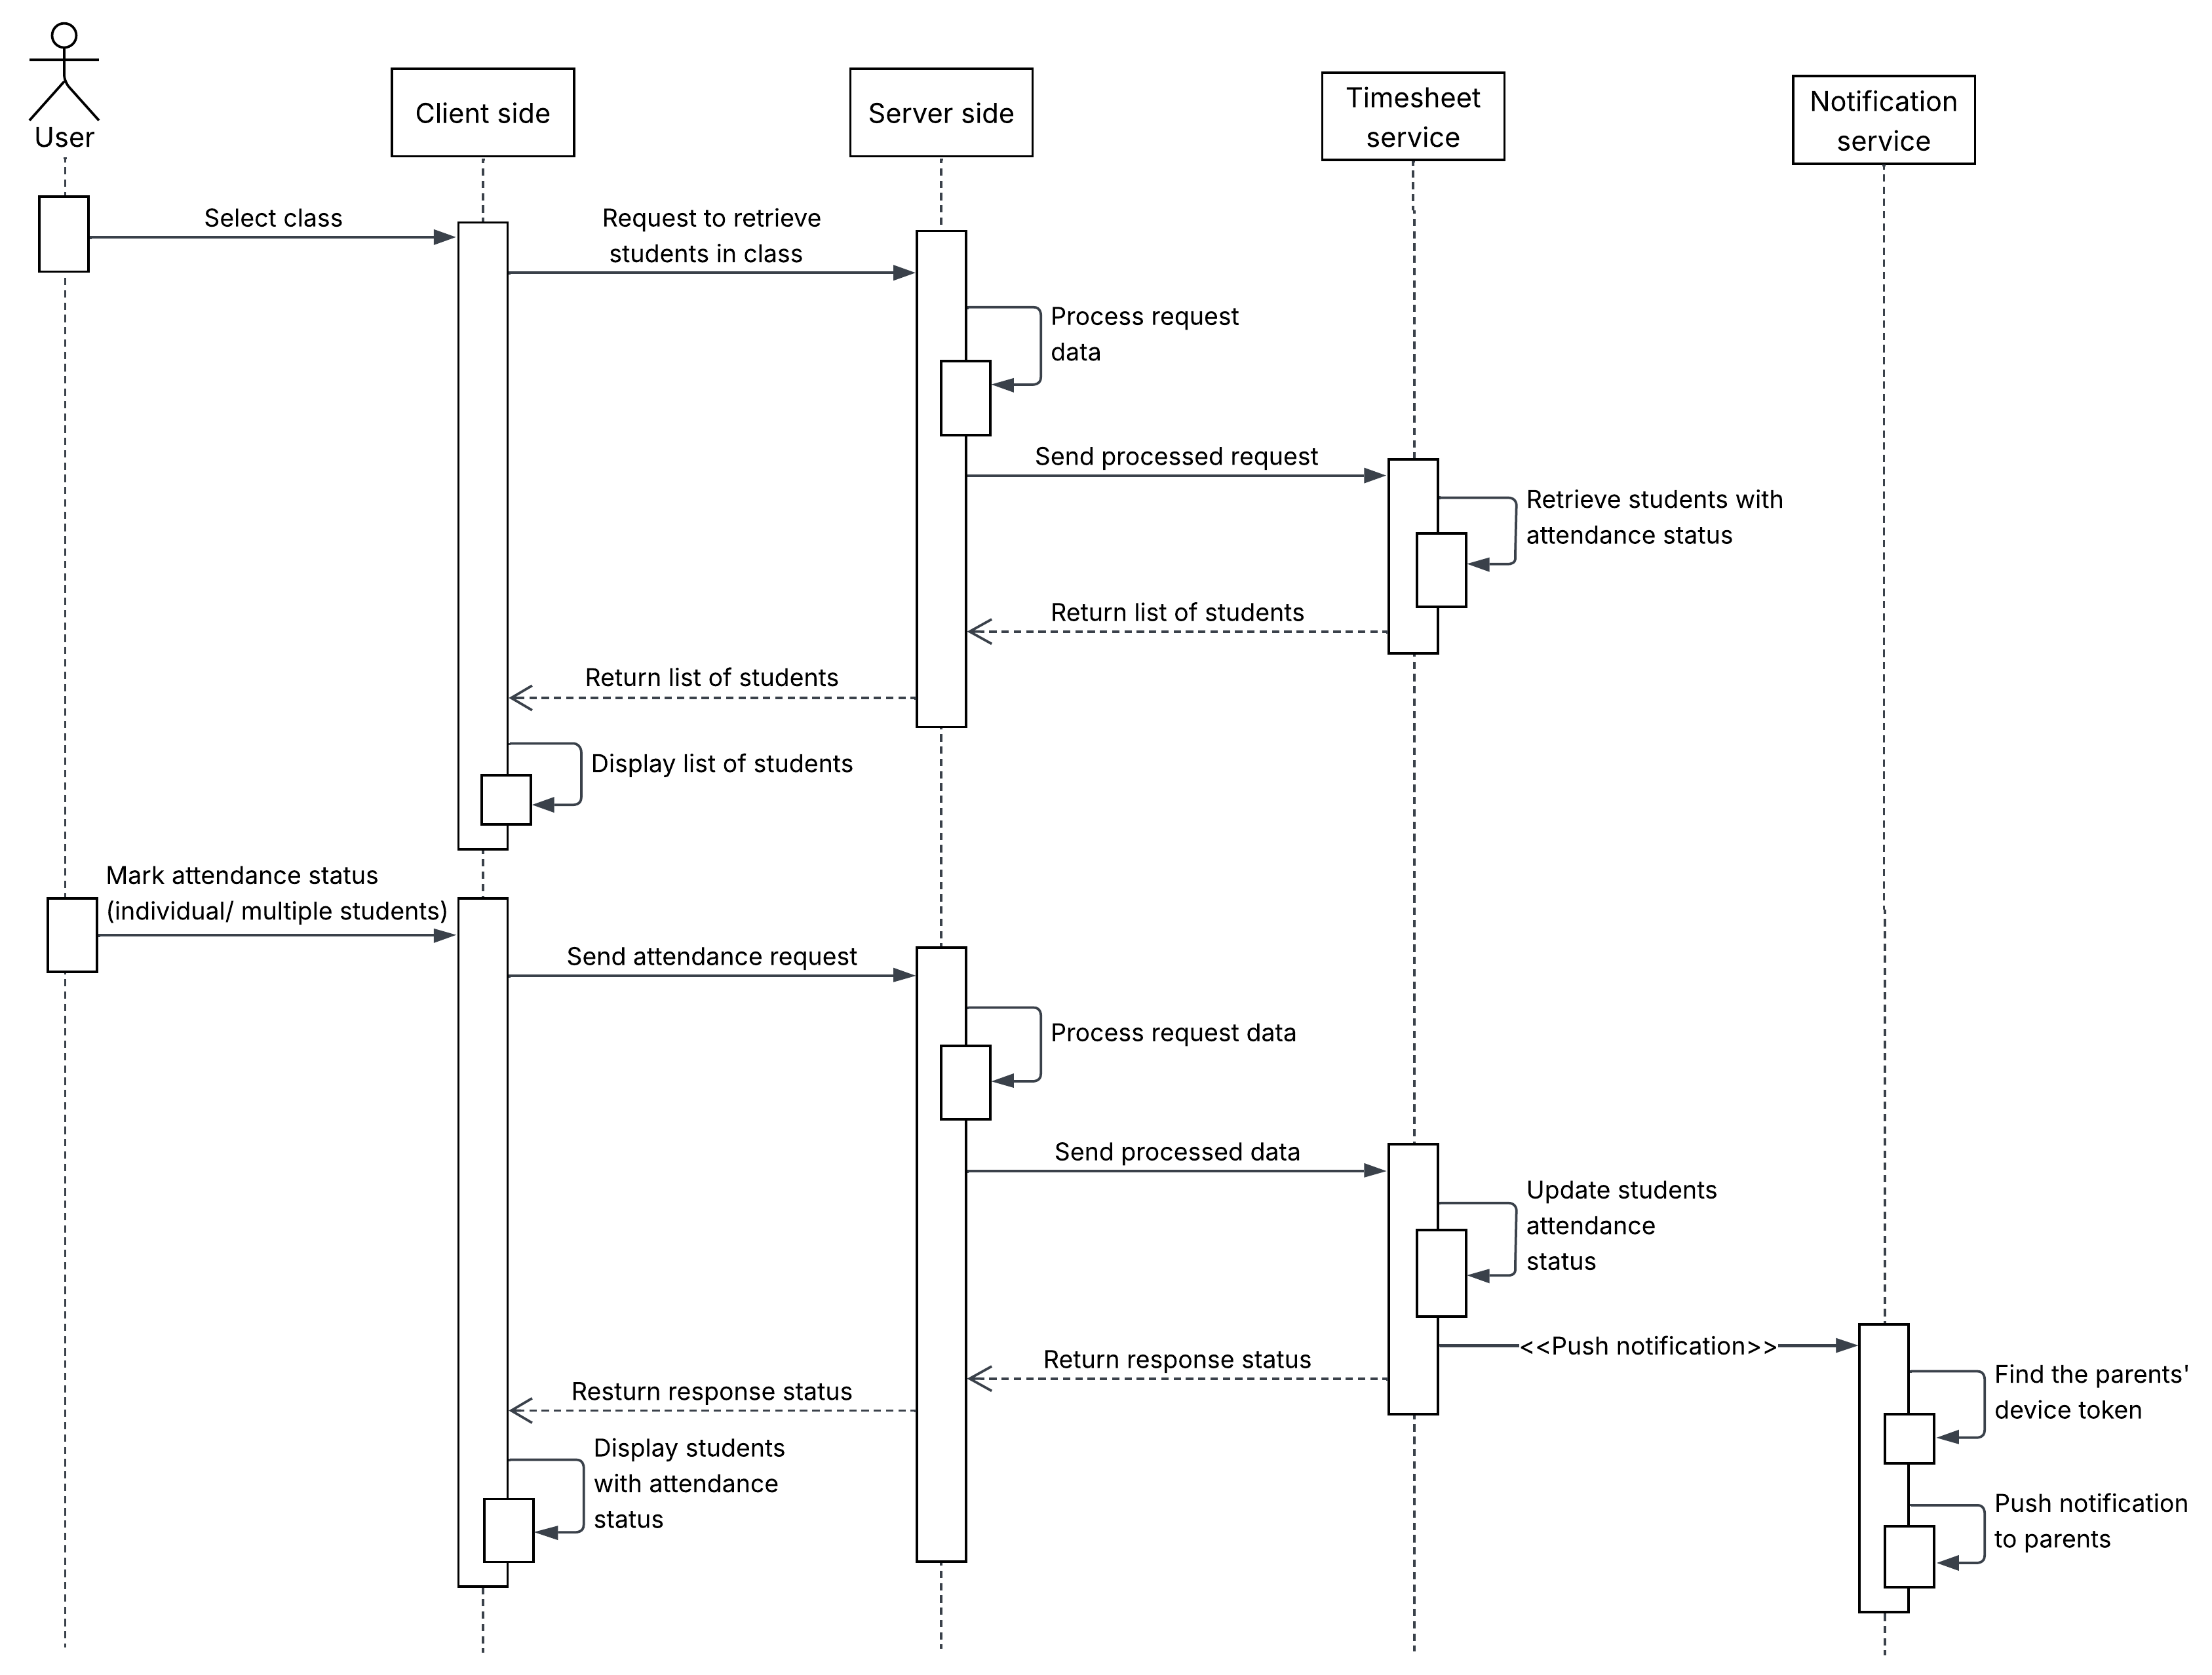
\includegraphics[width=1\textwidth]{images/sqd_mark_attendance_class.png}
    \vspace{-1em}
    \caption{Mark student presence sequence diagram.}
    \label{fig:sequence_diagram_mark_student_presence}
\end{figure}
\begin{minipage}{\textwidth}
    \setlength{\parindent}{2em}
    The sequence diagram illustrates a detailed process for marking student attendance in a classroom. When a user requests to mark attendance, the system retrieves a list of students in the class with their current attendance status (not marked, attended, absent, late, or left early). Users can update attendance records by marking individual students or multiple students simultaneously as present, absent, on excused leave, or having departed early. Once the attendance records are updated, the server asynchronously pushes notifications to parents.  
\end{minipage}

% IMPORT EMPLOYEE DATA
\subsubsection{Sequence Diagram for Import Employee Data}
\vspace{-1.5em}
\begin{figure}[H]
    \centering
    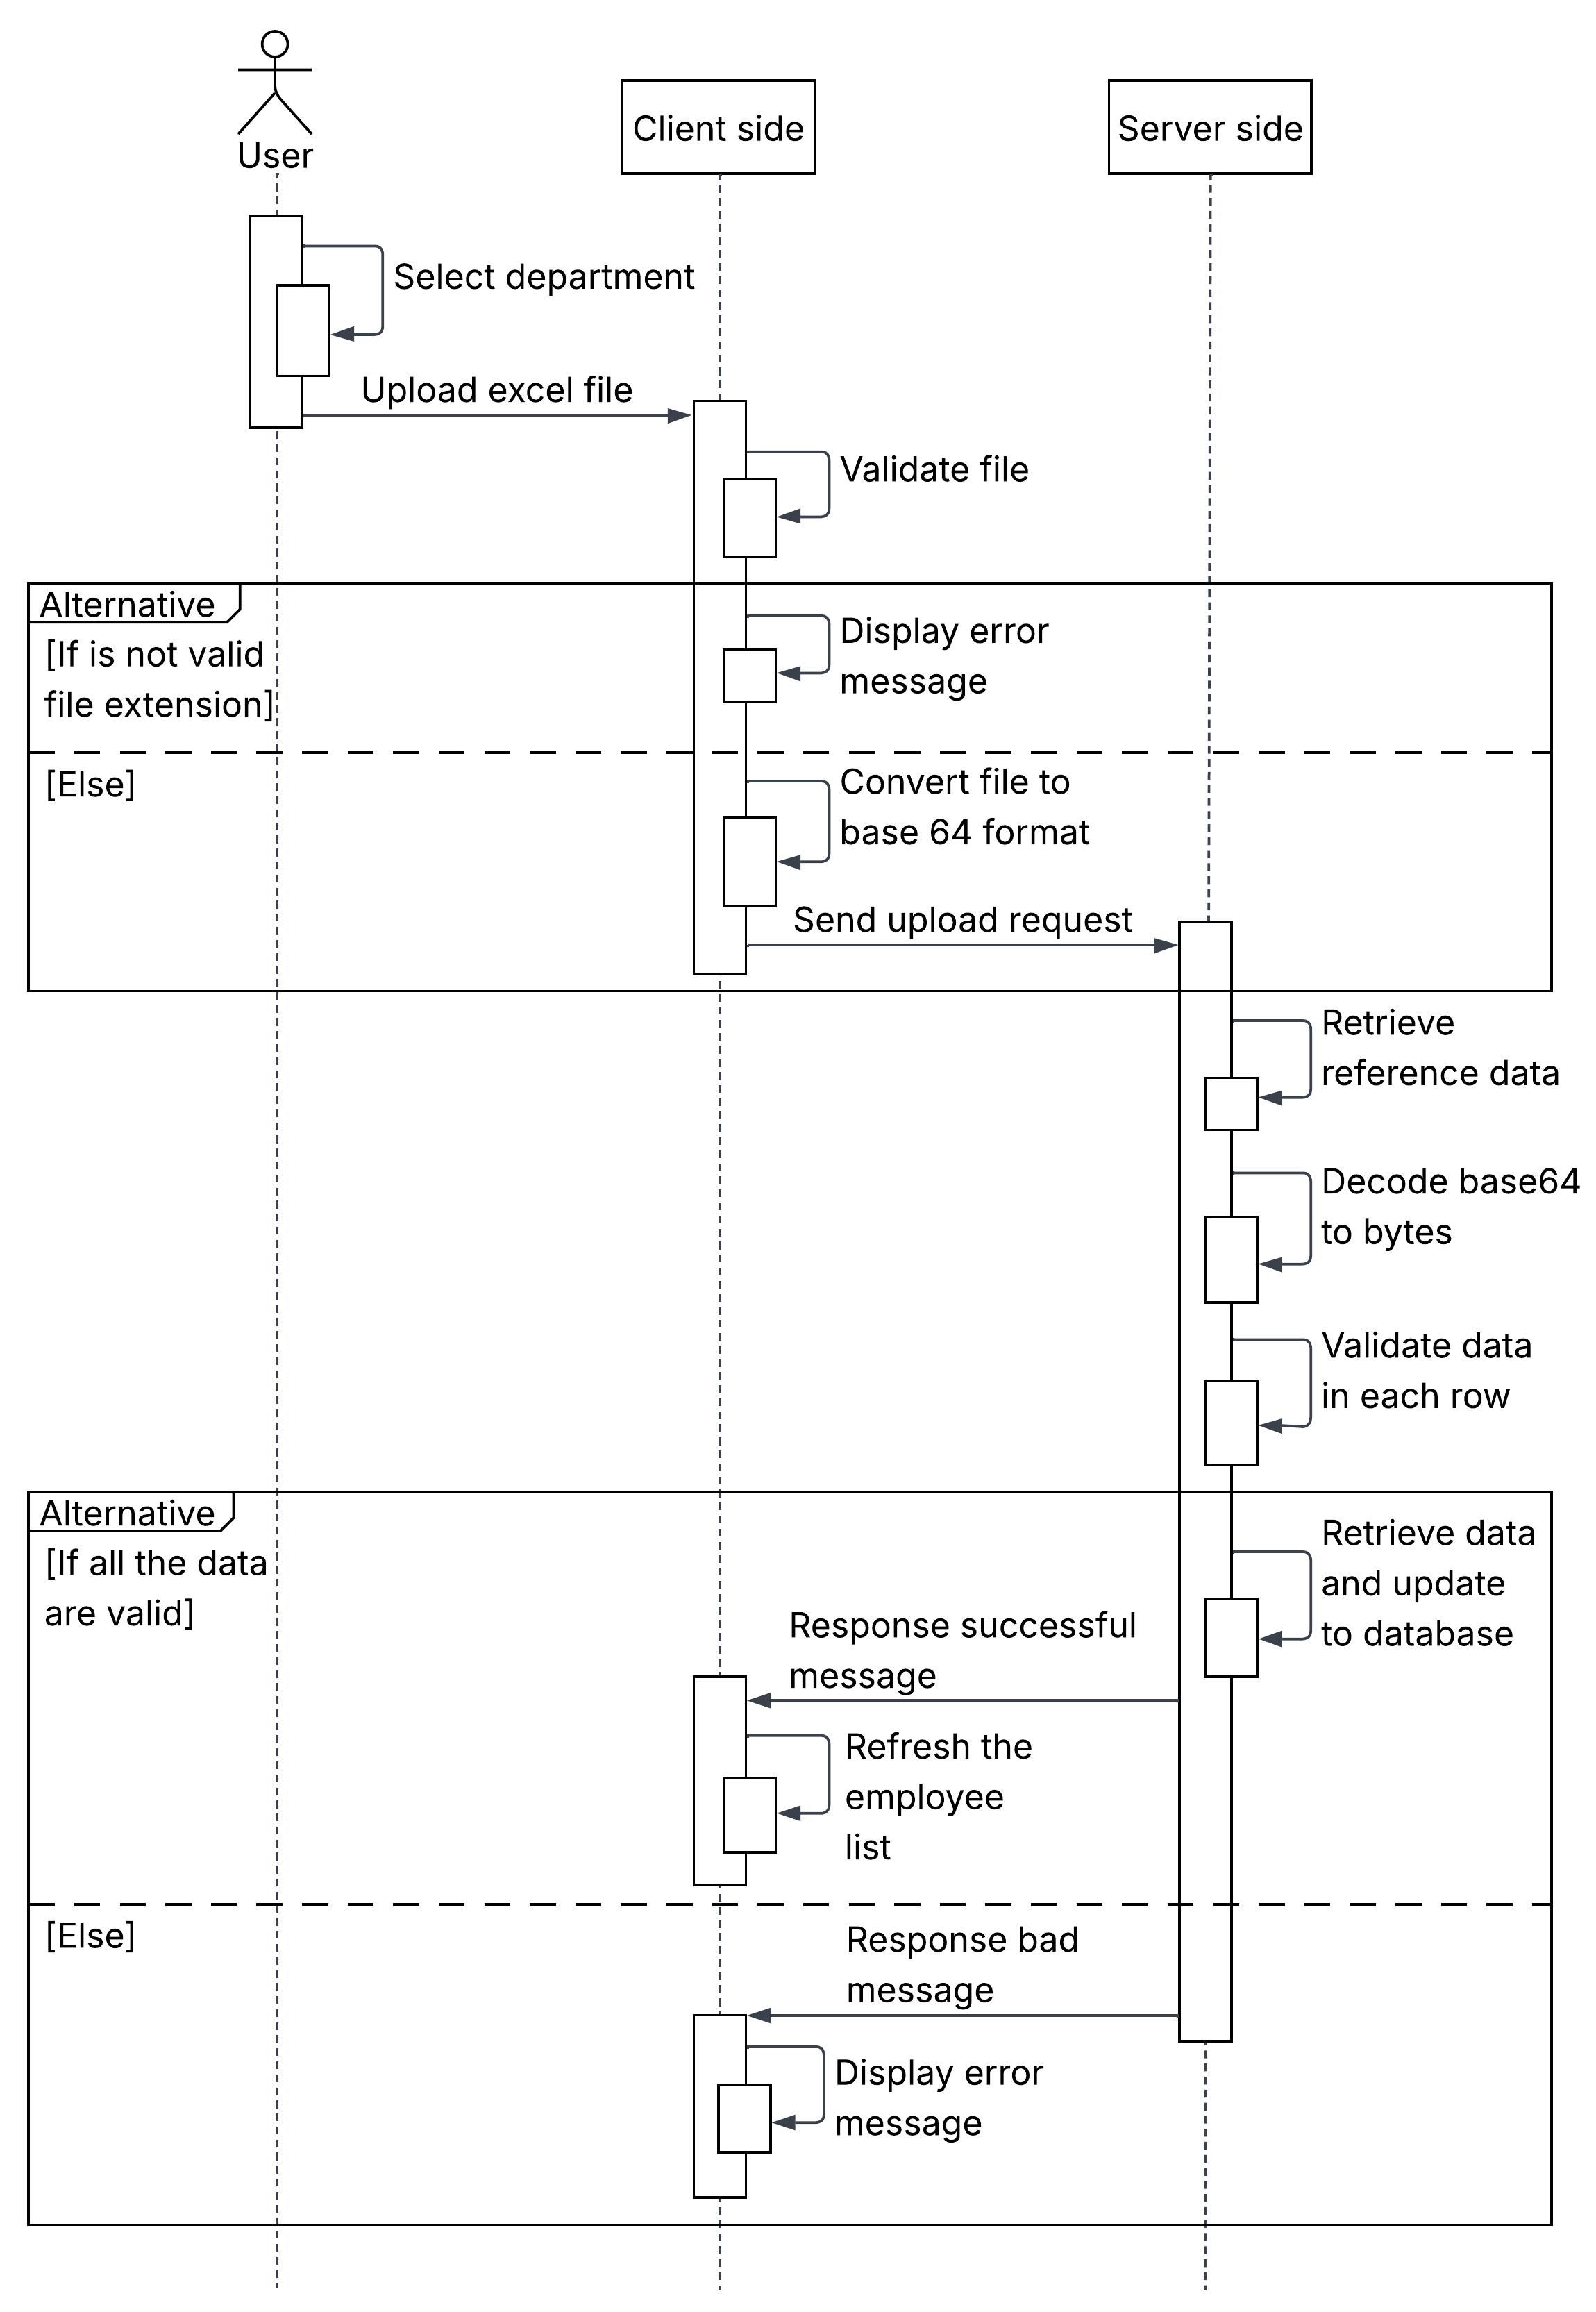
\includegraphics[width=0.8\textwidth]{images/sqd_import_employee_data.png}
    \vspace{-1em}
    \caption{Import employee data sequence diagram.}
    \label{fig:sequence_diagram_import_employee_data}
\end{figure}
\begin{minipage}{\textwidth}
    \setlength{\parindent}{2em}
    The sequence diagram illustrates a detailed process for importing employee data into the system. The user selects the department and uploads an employee Excel file. The client-side validates the format of the uploaded file. If the file format is invalid, it displays an error message to the user. Otherwise, it encodes the file to base64 format and sends a request to the server side. The server retrieves necessary reference data, decodes the file into bytes, and reads the content. The server then validates each row of data individually. If all the data is valid, the systems update the data to the database. However, if any data is invalid, it responds bad message to the user.
\end{minipage}

% CREATE LEAVE REQUEST
\subsubsection{Sequence Diagram for Create Student Leave Request}
\vspace{-1.5em}
\begin{figure}[H]
    \centering
    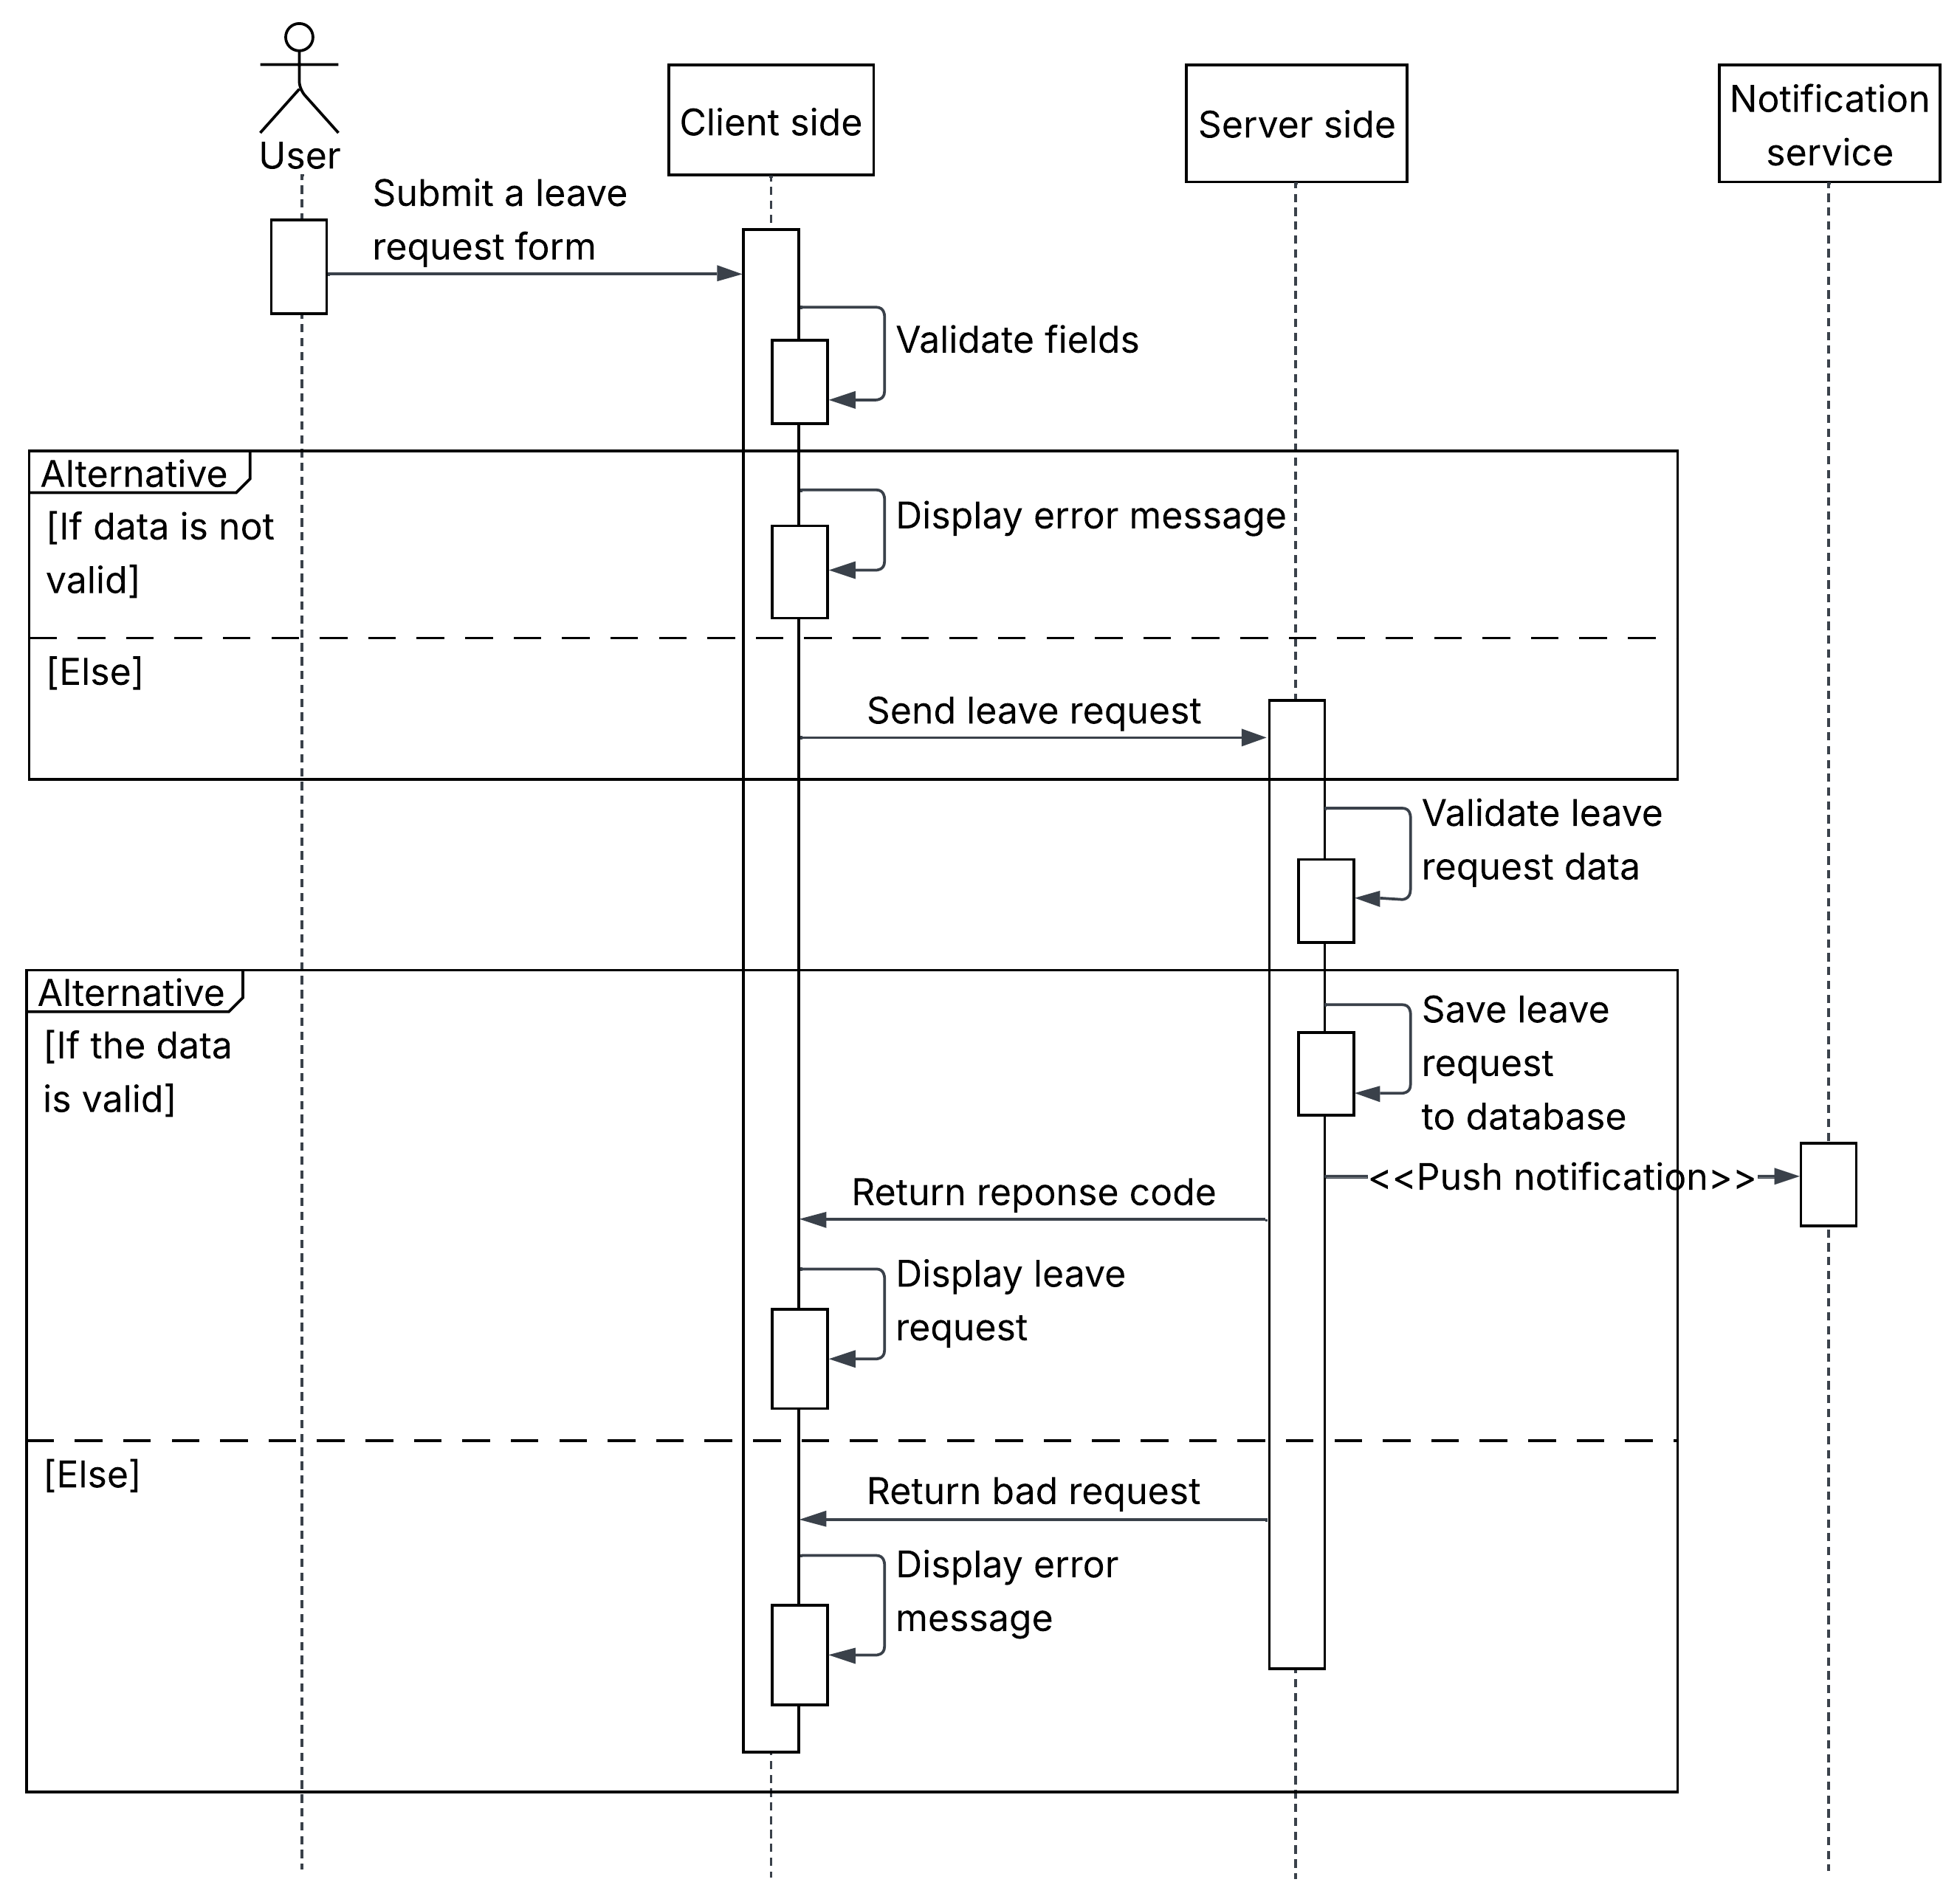
\includegraphics[width=1\textwidth]{images/sqd_create_student_leave_request.png}
    \vspace{-1em}
    \caption{Create student leave request sequence diagram.}
    \label{fig:sequence_diagram_create_student_leave_request}
\end{figure}
\begin{minipage}{\textwidth}
    \setlength{\parindent}{2em}
    The sequence diagram illustrates the operation when parents create a leave request for their child. First, they fill in all the required fields in the forms. The system checks these fields on the client side to make sure the information is valid. If everything is correct, the request is sent to the server. On the server side, the system performs further checks to prevent duplicate requests, such as overlapping dates or requests during holidays. Once the request passes all validations, it is saved to the database, and a notification is sent to the teacher. This process helps parents efficiently submit and track leave requests while ensuring teachers are promptly informed of planned student absences.
\end{minipage}

% CONFIRM LEAVE REQUEST
\subsubsection{Sequence Diagram for Confirm Student Leave Request}
\vspace{-1.5em}
\begin{figure}[H]
    \centering
    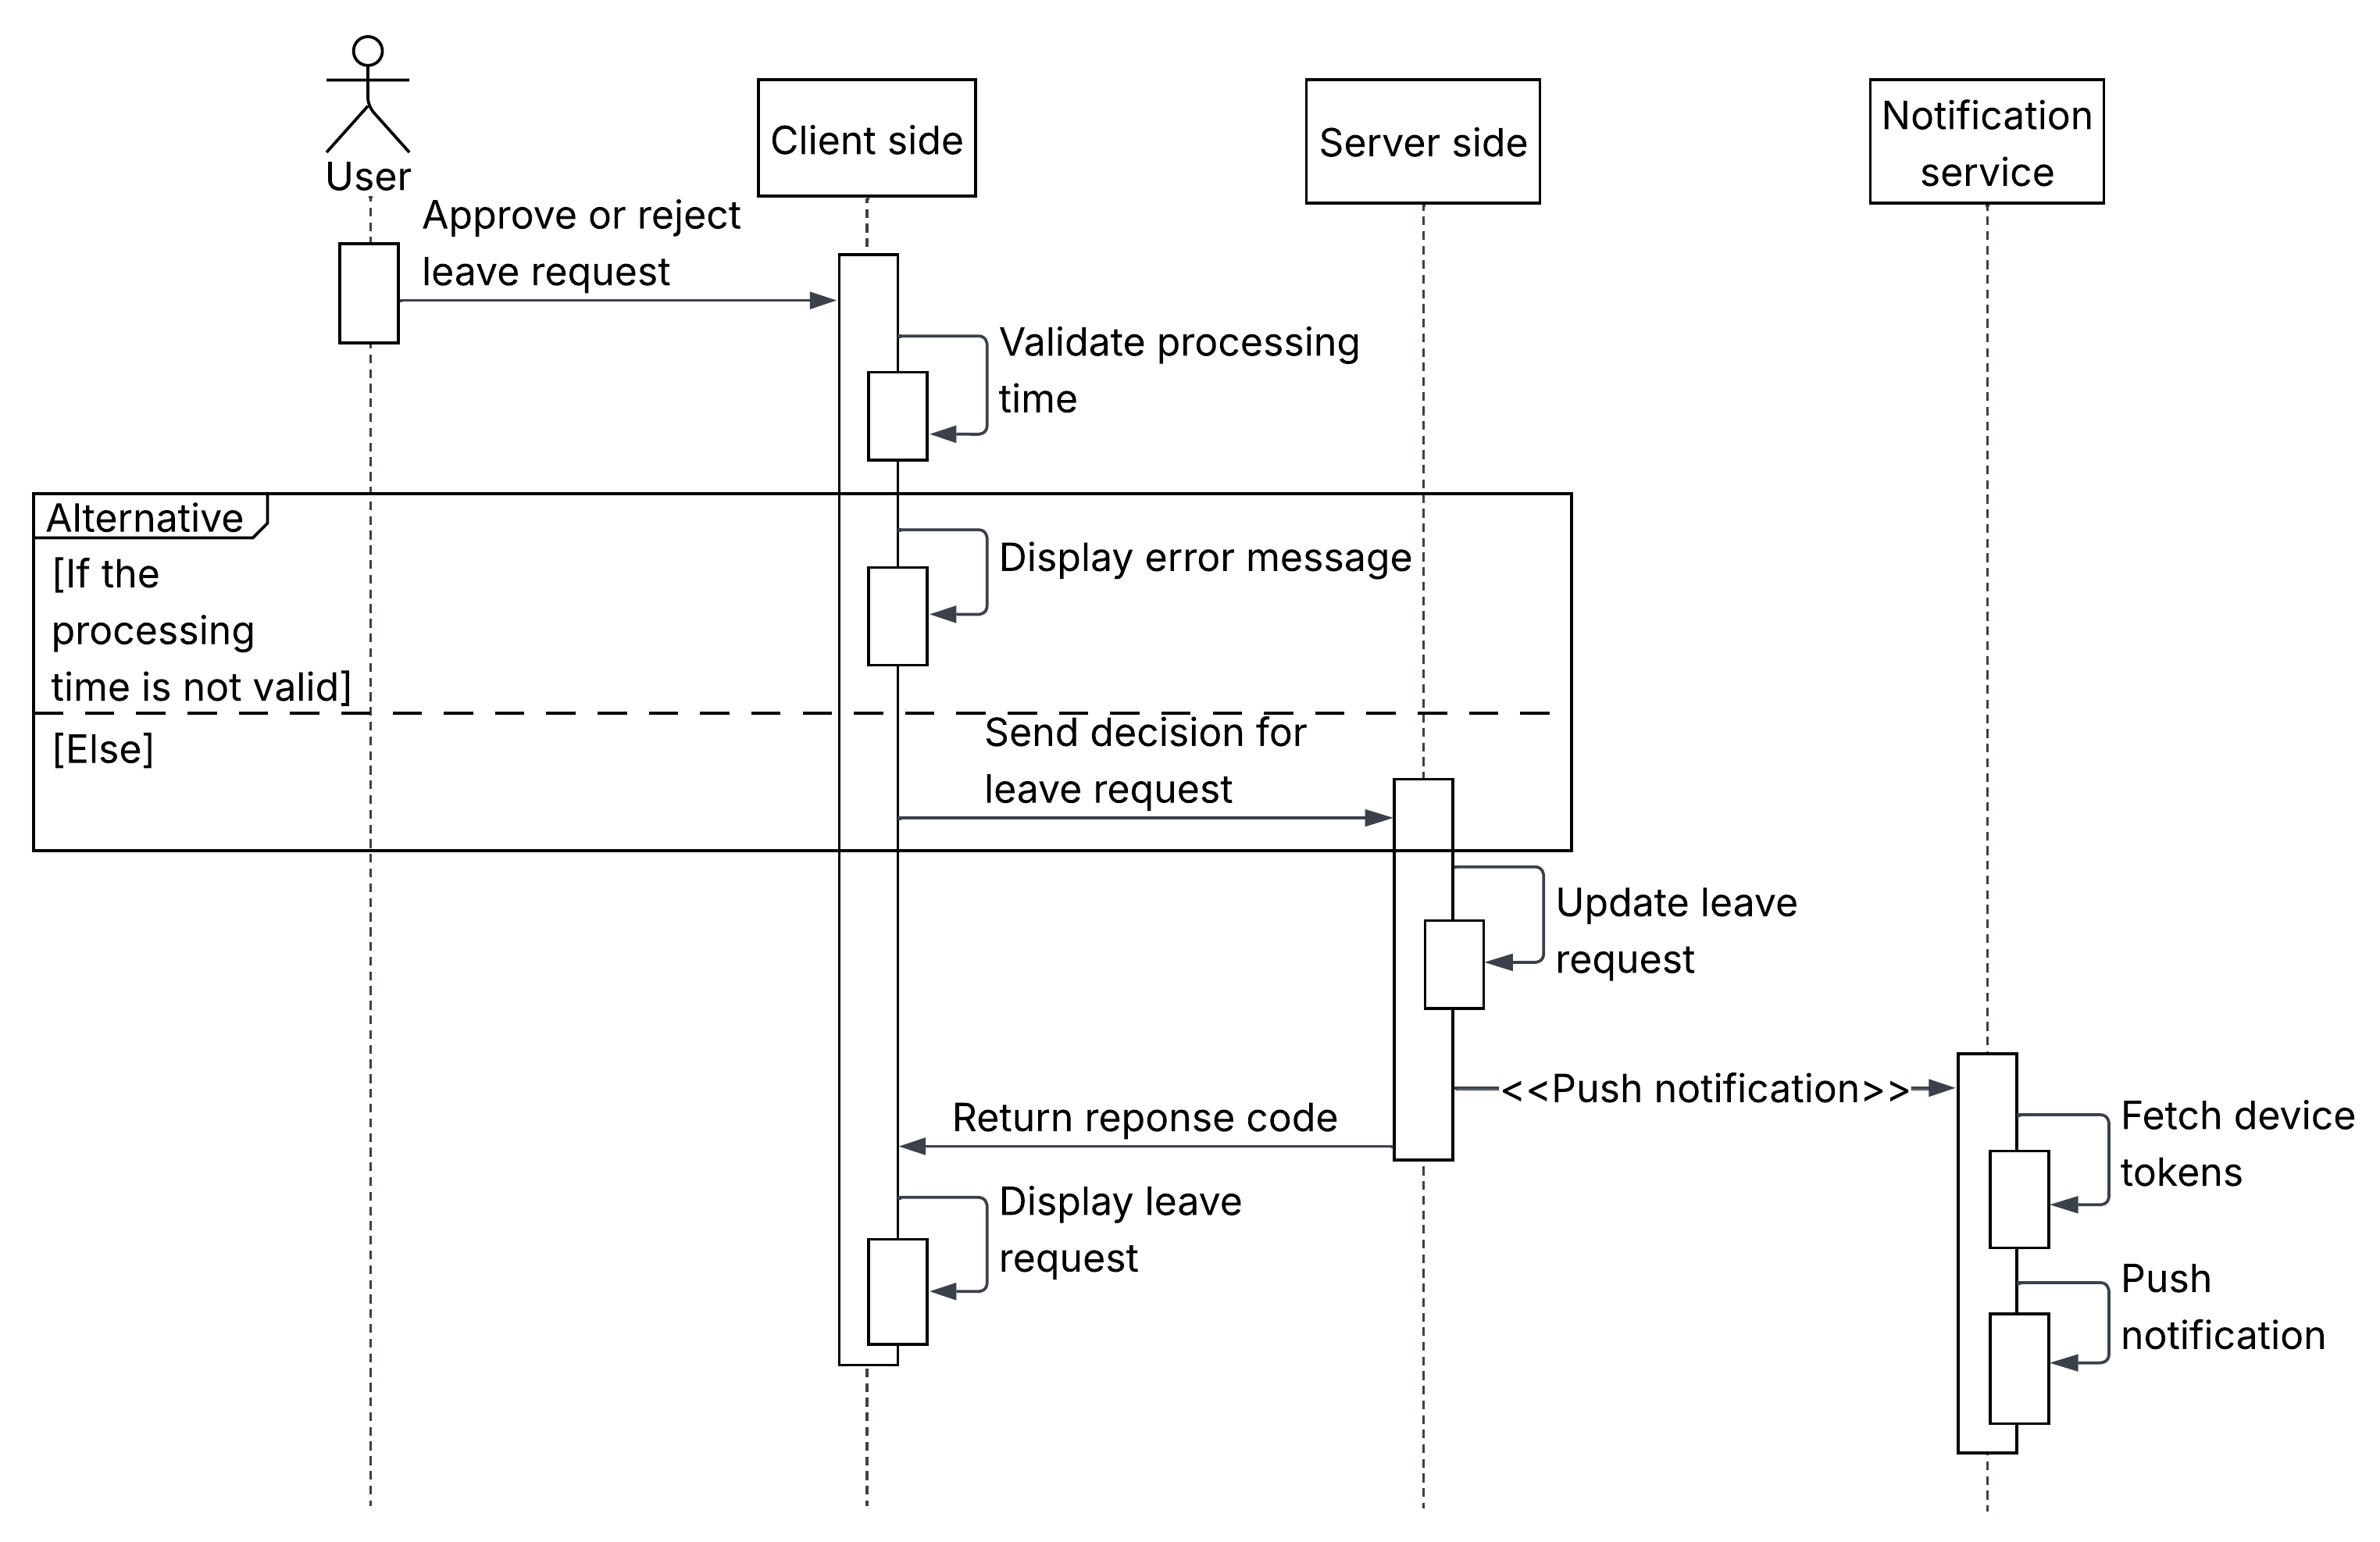
\includegraphics[width=1\textwidth]{images/sqd_confirm_student_leave_request.png}
    \vspace{-1em}
    \caption{Confirm student leave request sequence diagram.}
    \label{fig:sequence_diagram_confirm_student_leave_request}
\end{figure}
\begin{minipage}{\textwidth}
    \setlength{\parindent}{2em}
    The sequence diagram illustrates the operation when teachers confirm or reject student leave requests. First, the client side checks the date range of the leave request. If the confirmation date is after or outside the leave request date range, teachers cannot confirm or reject the request. Otherwise, they can proceed with their decision. Next, the decision for the leave request is sent to the server, which updates the leave request status, records the confirming teacher's information, and pushes notifications to parents. Once the process is successful, parents can view the updated leave request status. This process makes it easier for teachers to quickly review and approve student leave requests, with all details properly recorded.
\end{minipage}

% CREATE NEWSFEED POST
\subsubsection{Sequence Diagram for Post Newsfeed}
\vspace{-1.5em}
\begin{figure}[H]
    \centering
    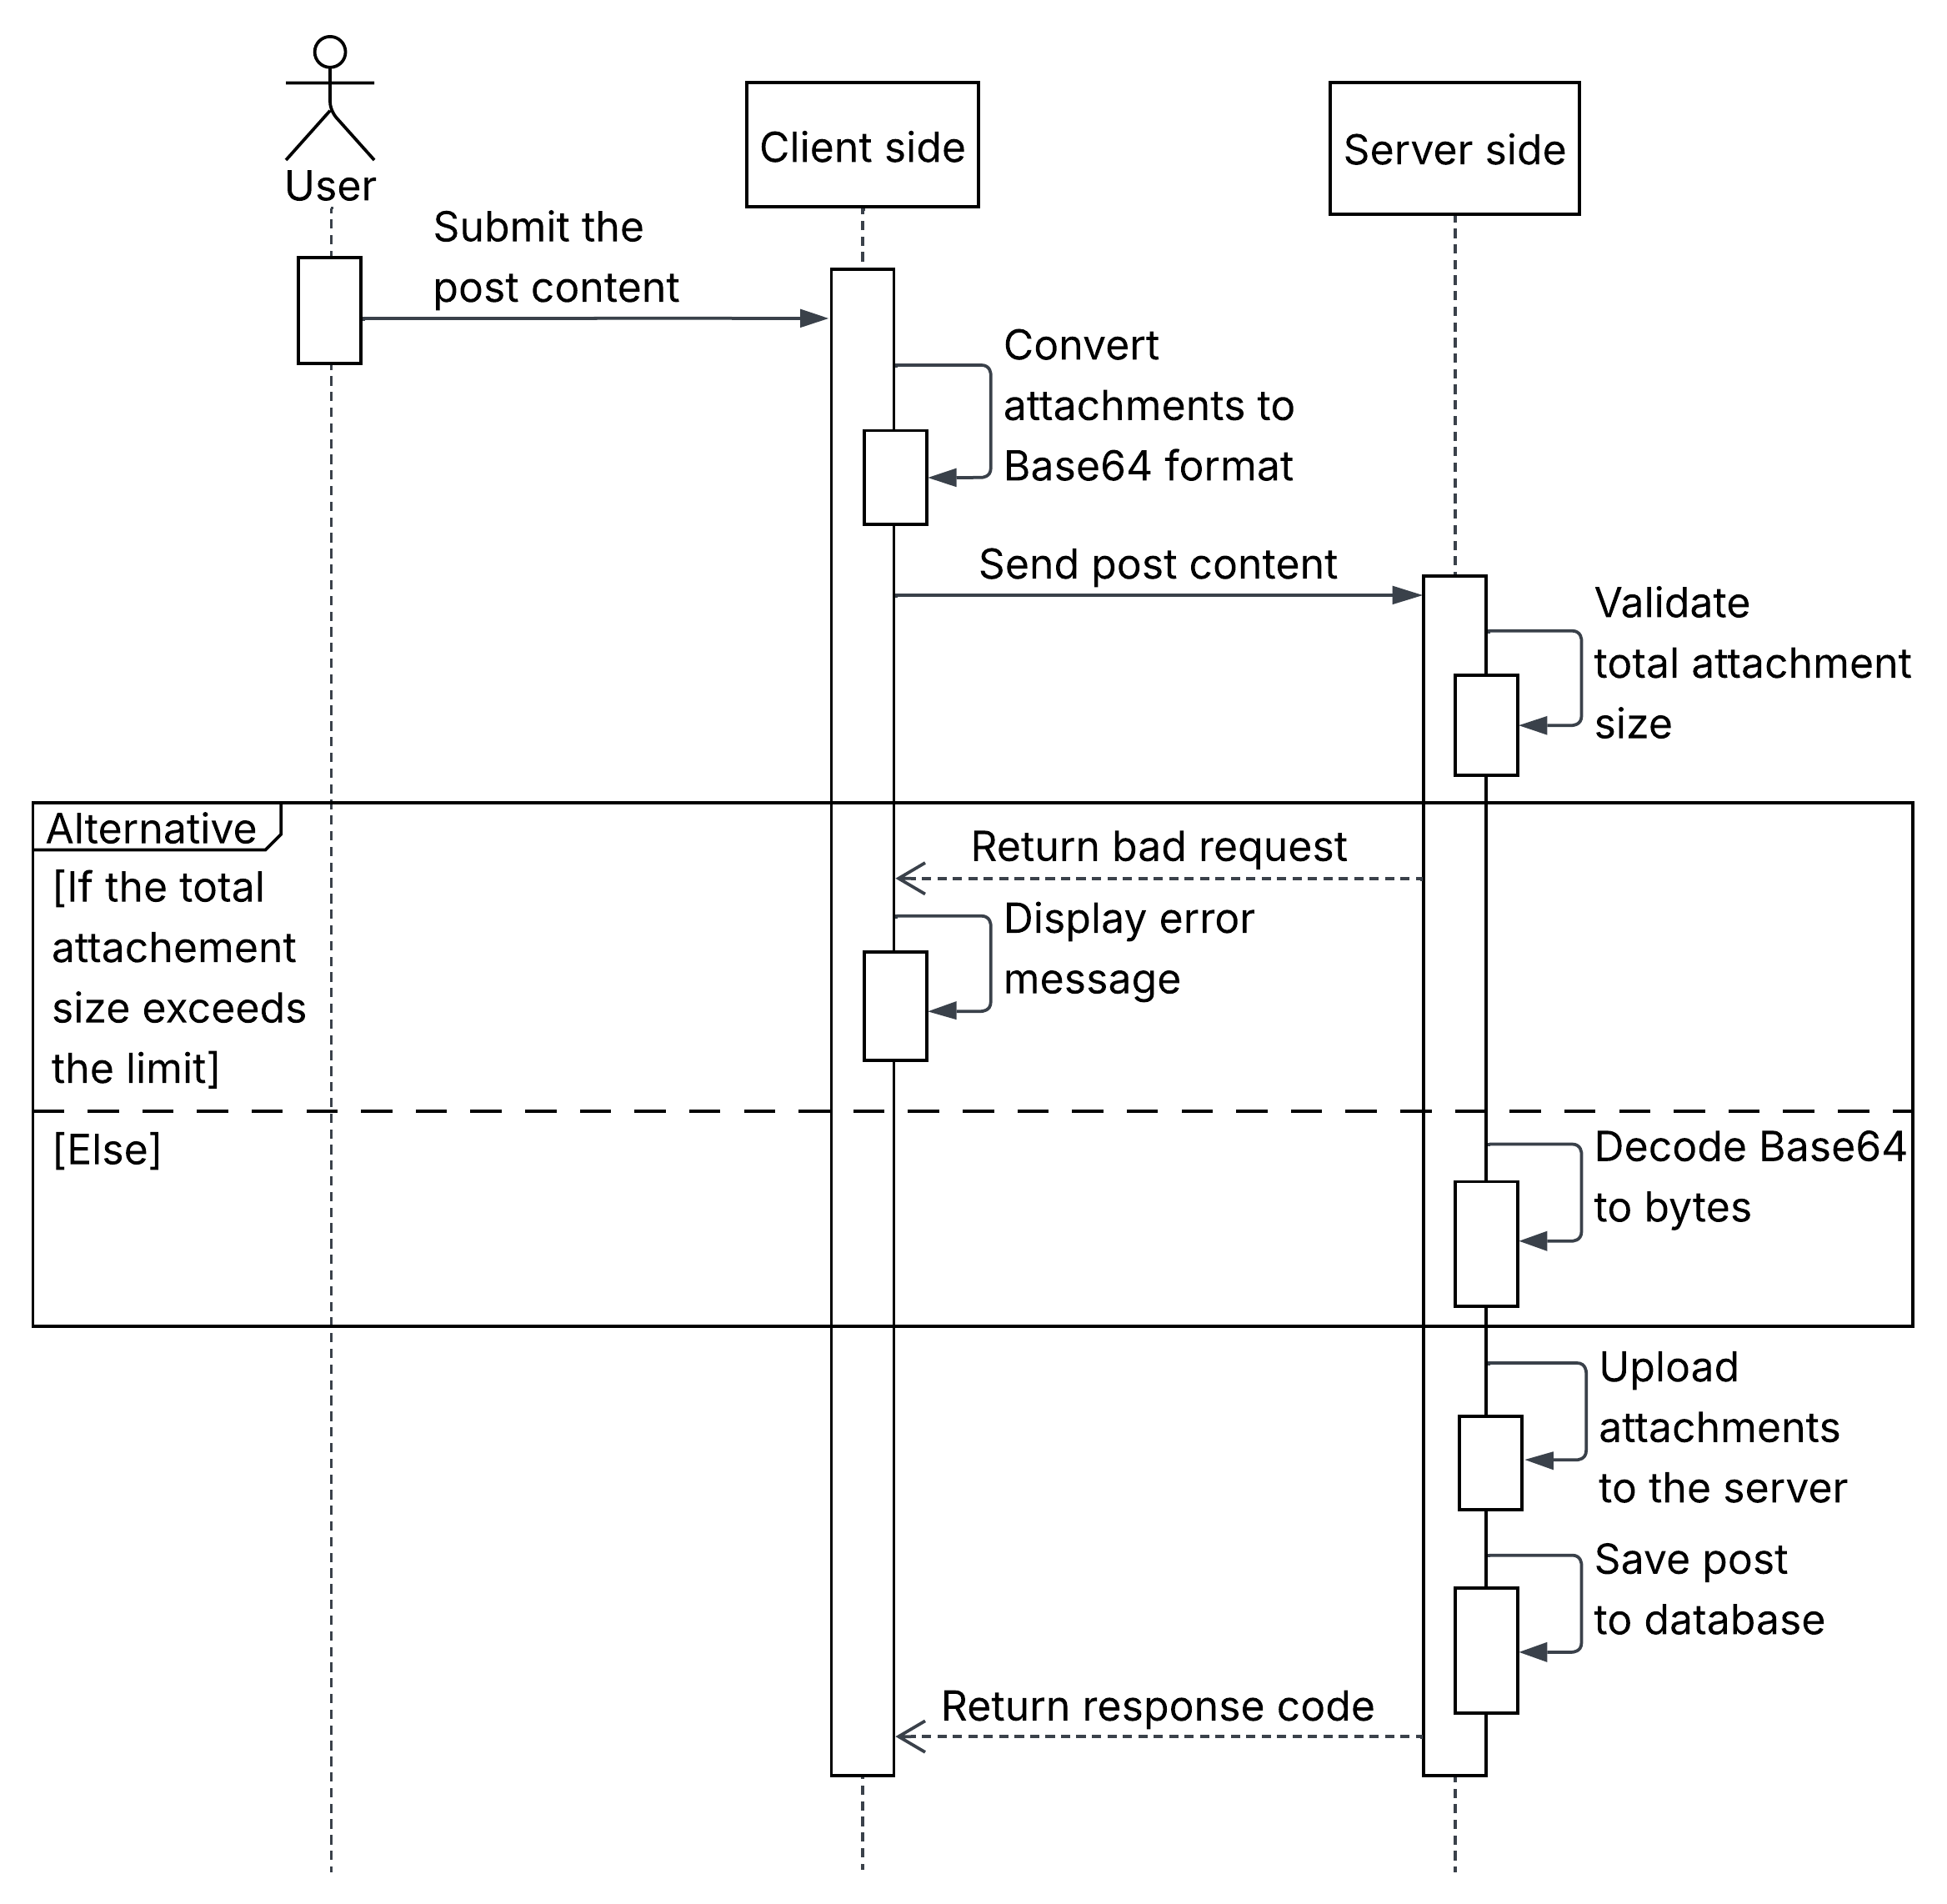
\includegraphics[width=1\textwidth]{images/sqd_post_newsfeed.png}
    \vspace{-1em}
    \caption{Post newsfeed sequence diagram.}
    \label{fig:sequence_diagram_post_newsfeed}
\end{figure}
\begin{minipage}{\textwidth}
    \setlength{\parindent}{2em}
    The sequence diagram illustrates the flow of actions when a teacher posts a newsfeed to the class. When a teacher creates a newsfeed post, the client-side application processes the content and converts any attachments to base64 format for transmission. After that, the system receives a request from the client side and validates the post. If the total attachment size does not exceed the limit, the system decodes the attachments to bytes, uploads the attachments to the server storage, and saves the post content to the database. Once processing is complete, the post is created and all student parents can view and interact with the post, enabling them to stay informed about their child's classroom and school activities.
\end{minipage}

% TRACK BUSES
\subsubsection{Sequence Diagram for Track Buses}
\vspace{-1.5em}
\begin{figure}[H]
    \centering
    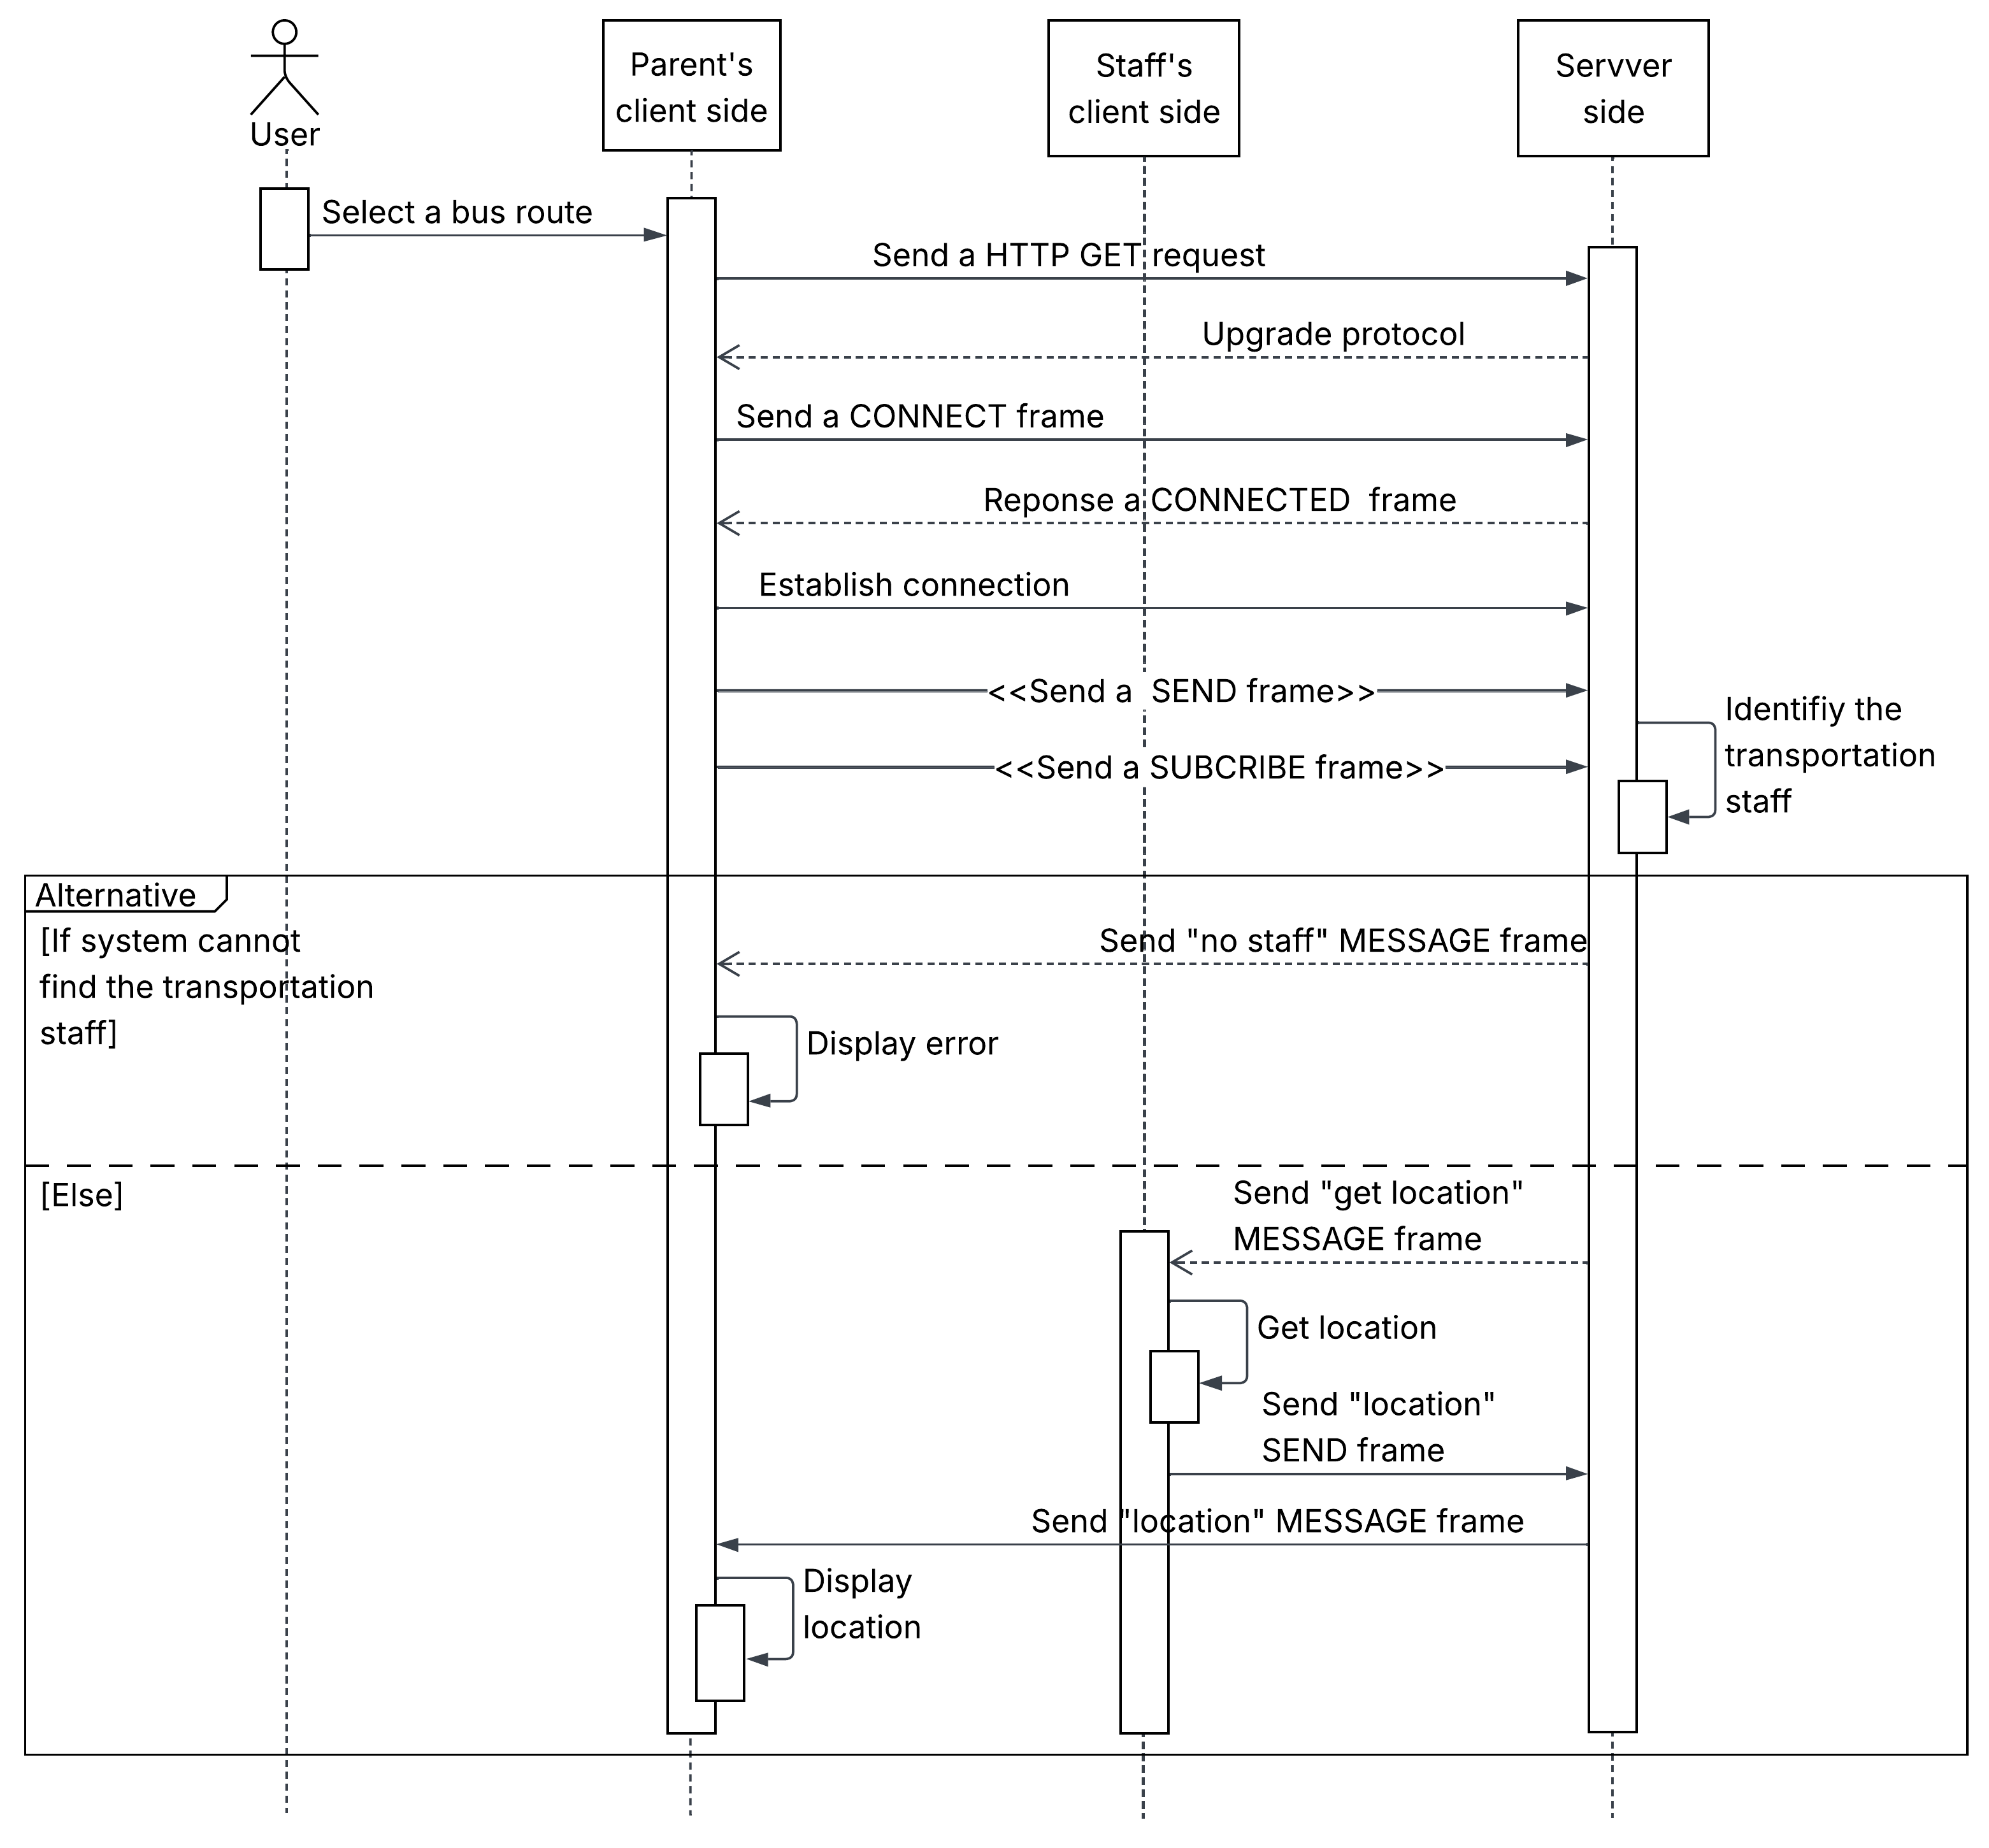
\includegraphics[width=1\textwidth]{images/sqd_track_bus.png}
    \vspace{-1em}
    \caption{Track buses sequence diagram.}
    \label{fig:sequence_diagram_track_buses}
\end{figure}
\begin{minipage}{\textwidth}
    \setlength{\parindent}{2em}
    The sequence diagram illustrates the real-time bus tracking process that enables parents to monitor their children's school buses. The workflow begins when a parent selects a specific bus route, prompting the client to initiate a WebSocket connection via an HTTP GET request, followed by a STOMP CONNECT frame. Once connected, the parent's client side sends a SEND frame to request the transportation staff location and a SUBSCRIBE frame to receive live updates. The system checks if transportation staff is assigned to the selected route. If available, the server sends a MESSAGE frame to the staff, prompting them to share their location. The staff client then sends location updates every 50 meters via SEND frames, which the server broadcasts to all subscribed parents. If no staff is assigned, the system notifies the parent immediately.
\end{minipage}

  % % 2.7 Database design
  % \subsection{Database Design}
  % \begin{minipage}{\textwidth}
    \setlength{\parindent}{2em}
    Following the analysis of the system requirements, this section outlines the \textbf{database tables supporting the modules and features under my responsibility}. It provides both a high-level overview and detailed descriptions of the entities, their attributes, and their relationships.
\end{minipage}


\subsubsection{Extracted database tables}
\noindent
\begin{minipage}{\textwidth}
    \setlength{\parindent}{2em}
    This part illustrated the \textbf{high-level overview of the extracted database tables for modules and features under my responsibility} through the Entity-Relationship Diagram (ERD). The ERD visually represents the core entities, their attributes, and the relationships between them.
\end{minipage}
\begin{figure}[H]
    \centering
    % 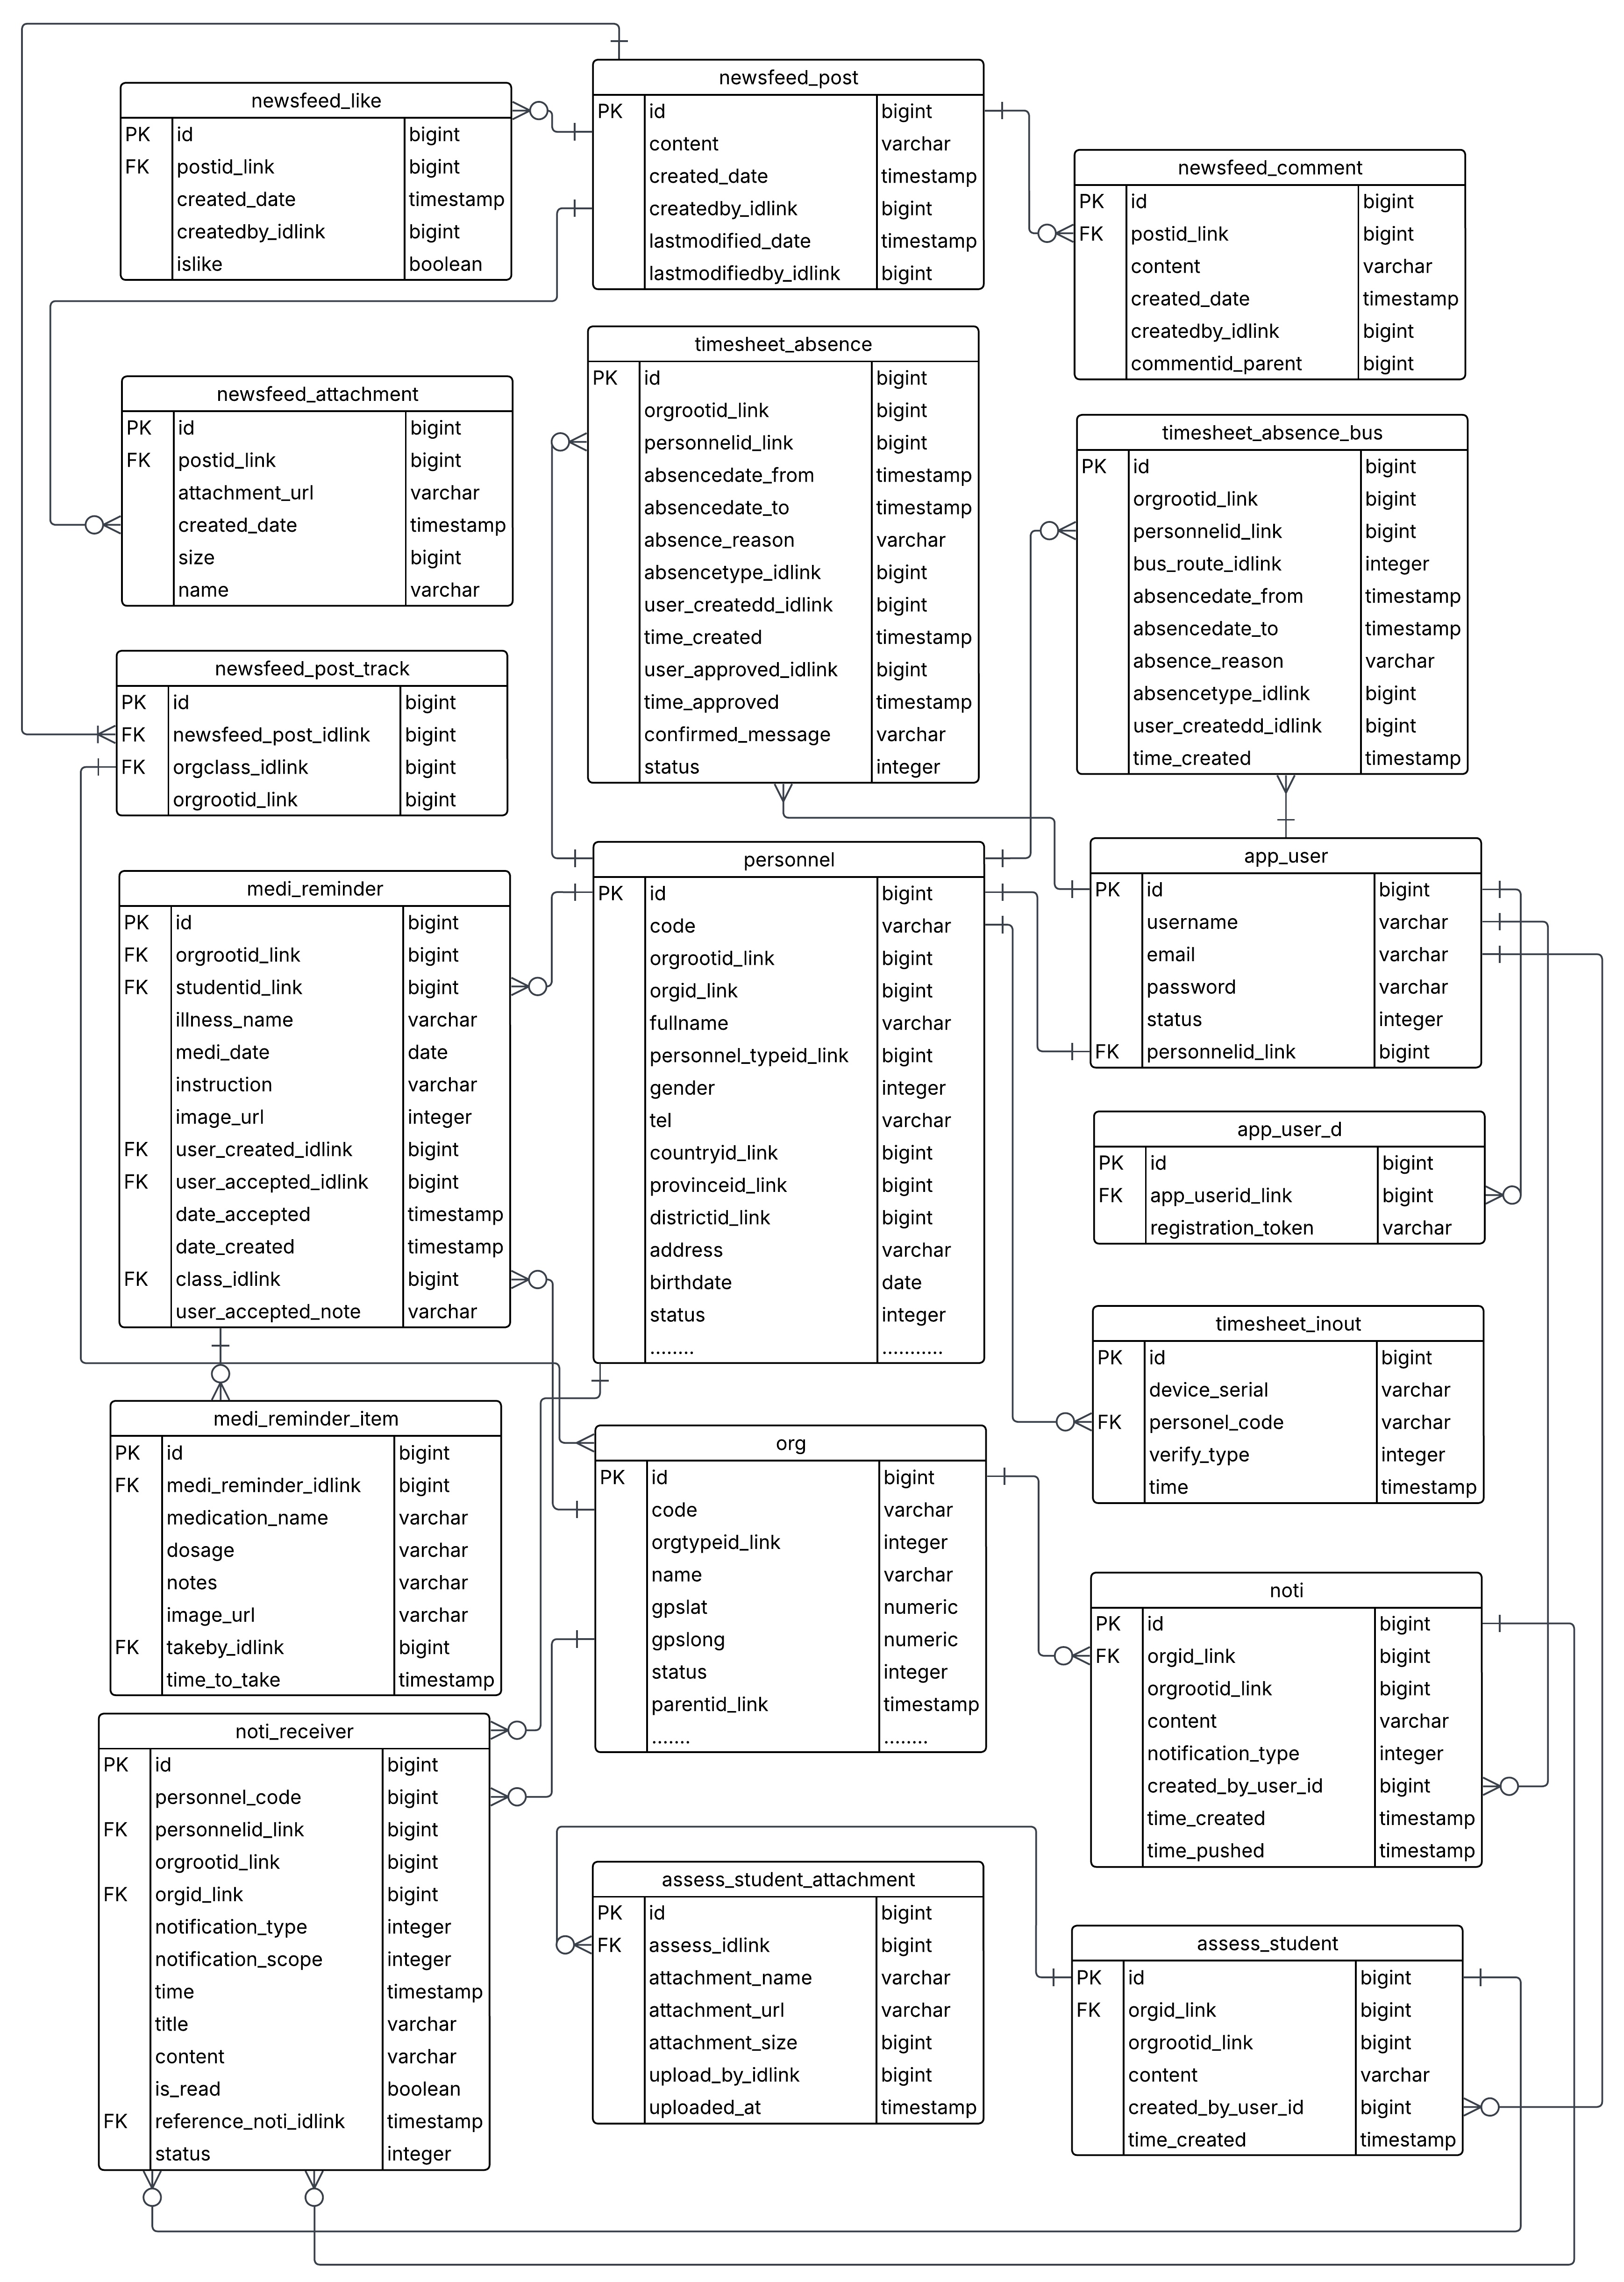
\includegraphics[width=1.05\textwidth]{images/database_erd.png}
    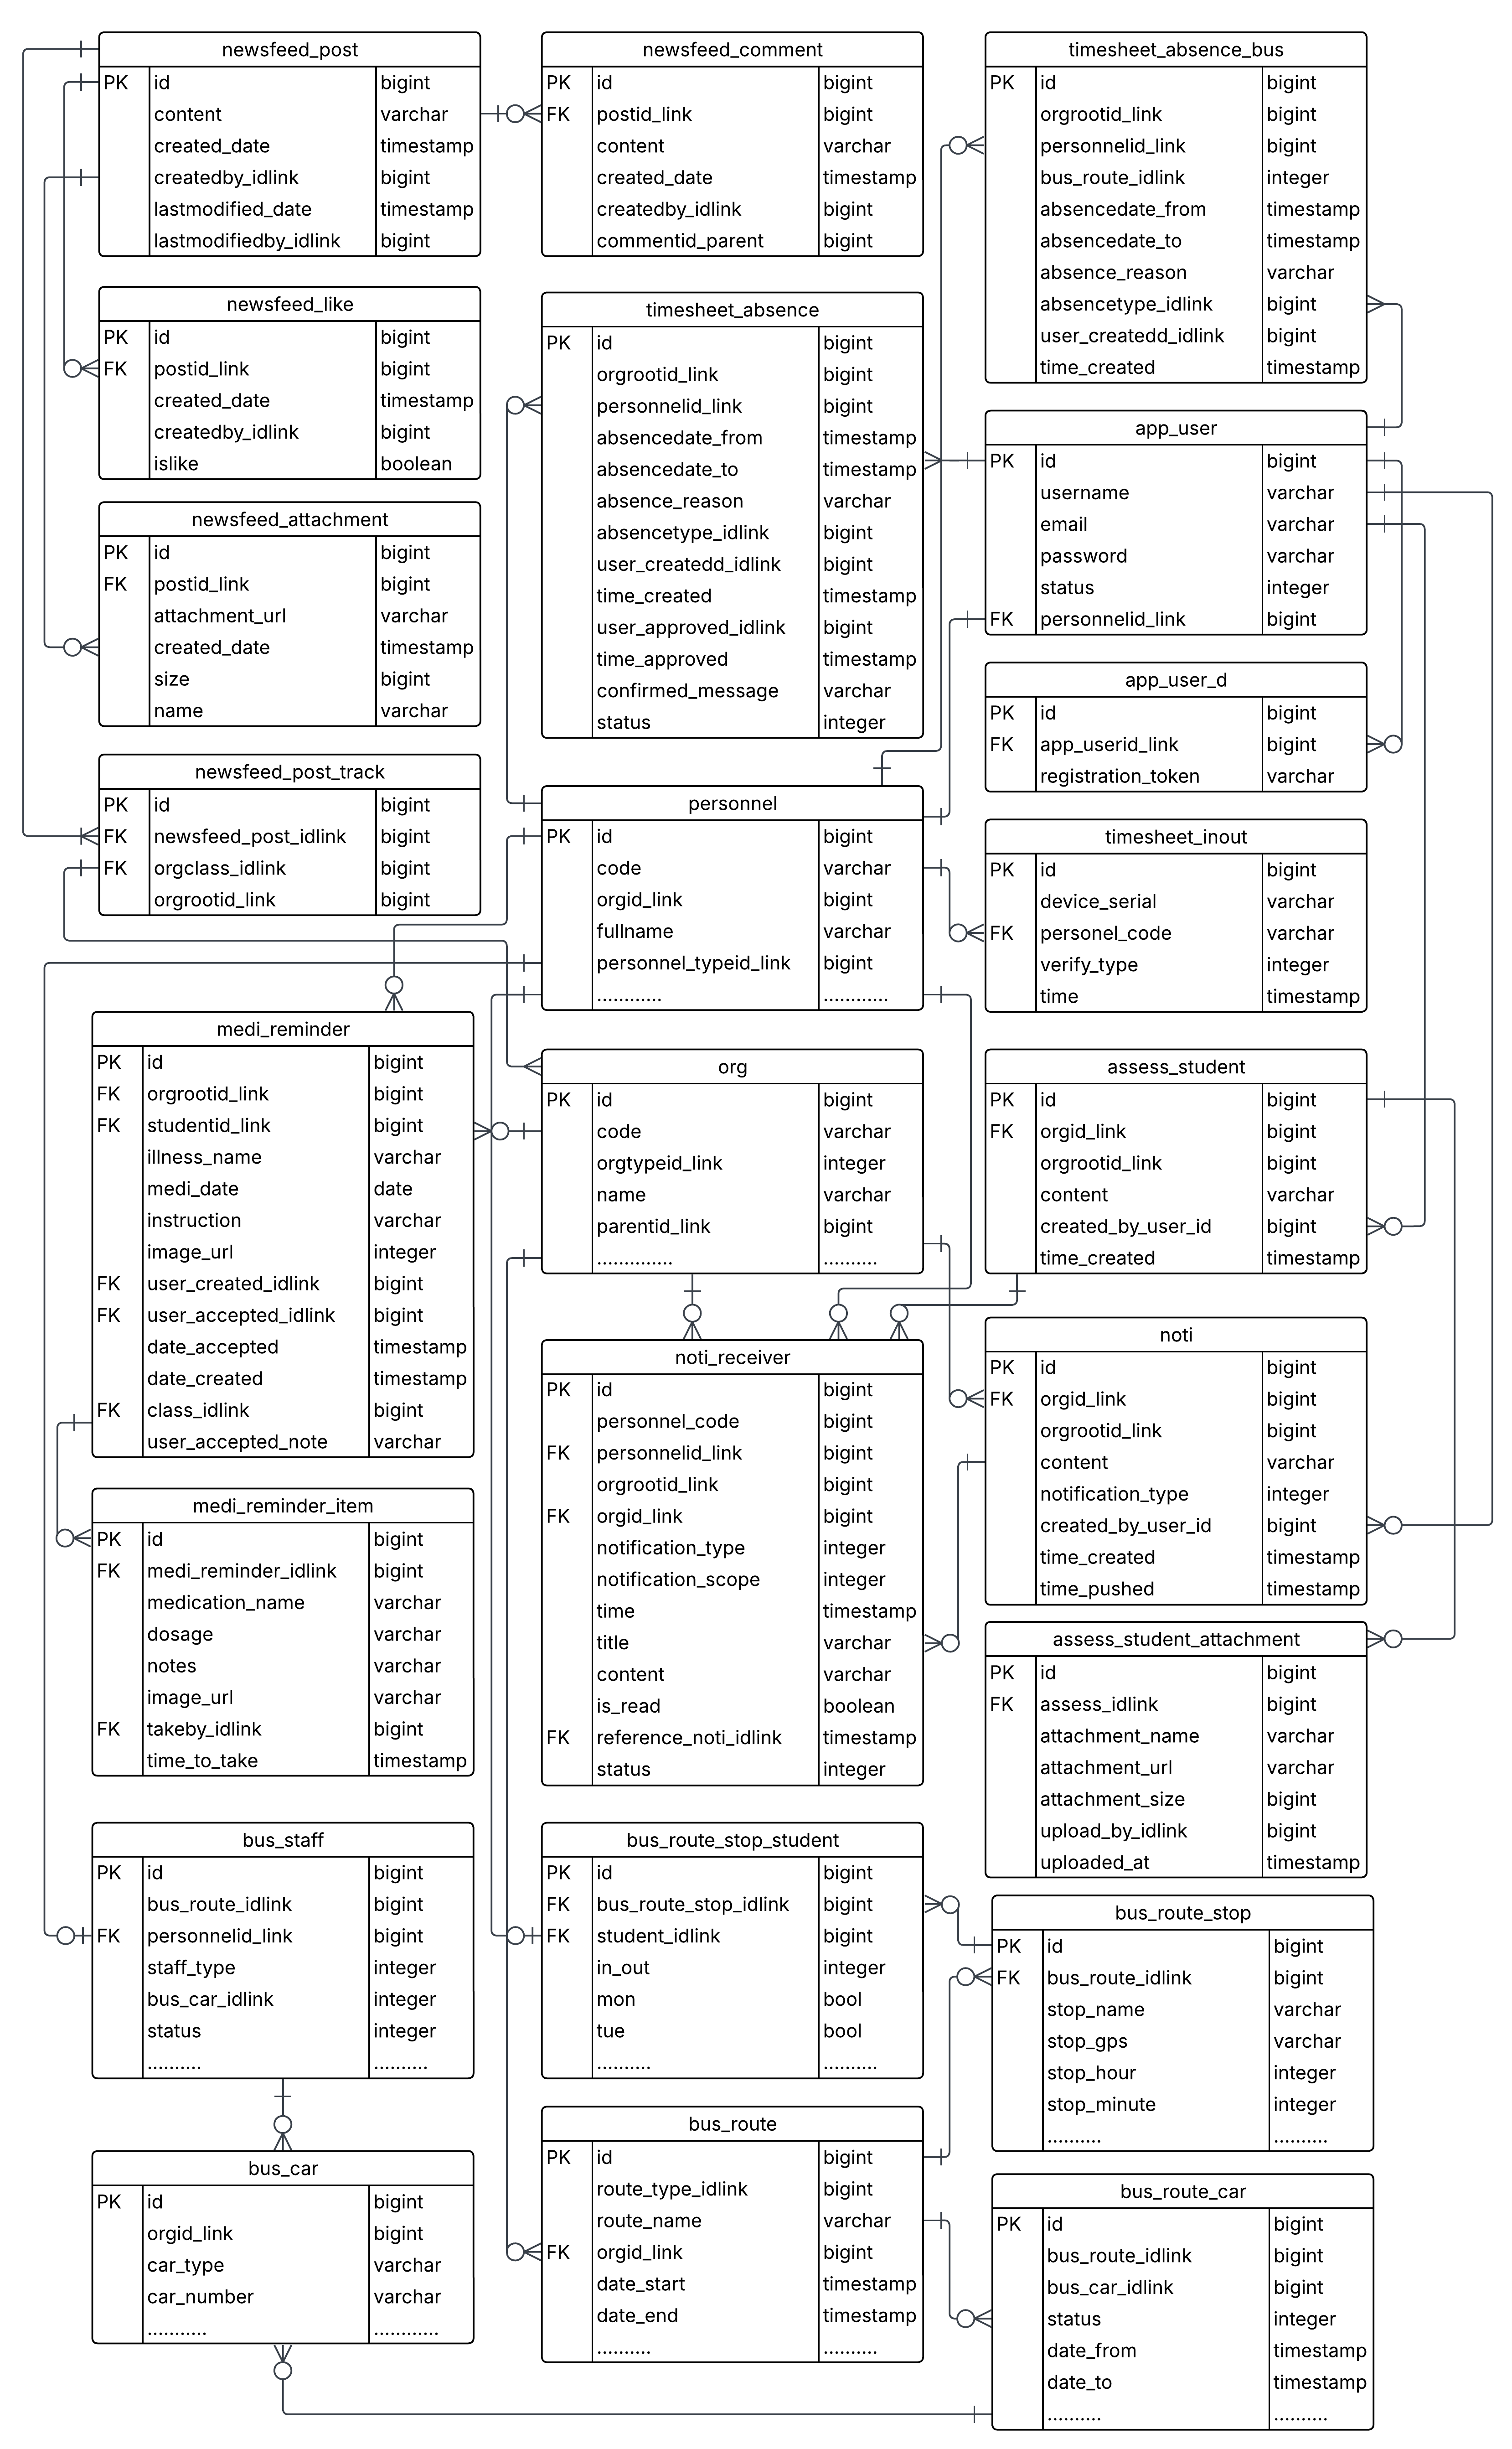
\includegraphics[width=1\textwidth]{images/image.png}
    \caption{Extracted database tables.}
    \label{fig:database_erd}
\end{figure}

\subsubsection{Database Design Description}
\noindent
\begin{minipage}{\textwidth}
    \setlength{\parindent}{2em}
    This section explain the \textbf{Extracted database tables} illustrated in \textbf{\autoref{fig:database_erd}} that related to the \textbf{features and modules assigned to me} in this project. Below is a detailed description of each entity and the relationships between them.
    % In this section, we will explain the Entity-Relationship Diagram (ERD) illustrated in \textbf{\autoref{fig:database_erd}} by describing each entity and its attributes, the relationships and cardinalities between entities, and how this design supports the system requirements.
\end{minipage}
\vspace{-0.8em}
\begin{itemize}[itemsep=-0.1cm]
    \item \textbf{personnel}: The table stores detailed information about both employees and students, which can be identified using the personnel\_typeid\_link attribute. It includes basic personal details (name, gender, birth date, contact, status) along with additional data specific to students and employees. This design ensures efficient management of personal information.
    \item \textbf{org}: The org table stores information about all organizational units (schools, departments, classes, etc) and uses the parentid\_link attribute to maintain a hierarchical structure.
    \item \textbf{app\_user}: This table stores user login credentials and controls access to the system. For security purposes, all passwords are encrypted using the Bcrypt hashing algorithm.
    \item \textbf{app\_user\_d}: The table manages mobile device access by linking each device token to a user account. These tokens are then used to send notifications.
    \item \textbf{timesheet\_inout}: The table is used to record raw attendance data. It tracks which device was used (device\_serial), the verification method: face recognition, fingerprint, or manual entry by a teacher (verify\_type), and the time when attendance was recorded.
    \item \textbf{timesheet\_absence}: Stores leave requests for employees and students. It records the absence dates, reason, leave type, and tracks the complete approval process including who submitted it, when it was created, who approved it, and approval time.
    \item \textbf{timesheet\_absence\_bus}: The table is used to track bus leave requests when students request time off from bus service, ensuring coordination between attendance and transportation management.
    \item \textbf{newsfeed\_post}: The main table for storing newsfeed content. Each post can be associated with multiple related entities, including newsfeed likes, comments, and attachments, enabling scalability.
    \item \textbf{newsfeed\_attachment}: The table manages attachments associated with newsfeed posts using URLs. It stores metadata like file name, size, and creation time, while the actual files are stored on the server and referenced by URLs.
    \item \textbf{newsfeed\_like}: The table manages user reactions to newsfeed posts, tracking which users have interacted with specific posts.
    \item \textbf{newsfeed\_comment}: The table manages user comments on newsfeed posts. It tracks who commented, the content, and timestamp while supporting hierarchical reply structures through the commentid\_parent field.
    \item \textbf{medi\_reminder}: The table stores the medicine reminders for students. It captures illness details, medication dates, treatment instructions, and tracks who created the reminder and which teacher confirmed it.
    \item \textbf{medi\_reminder\_item}: The table stores individual medicine details within each reminder request. These records maintain a direct relationship with their corresponding medication reminders through the medi\_reminder\_idlink.
    \item \textbf{assess\_student}: The assess\_student manages assessments for individual or multiple students.
    \item \textbf{assess\_student\_attachment}: The table manages file attachments associated with assessments using URLs. It stores metadata like file name, size, and creation time.
    \item \textbf{noti}: The table stores notifications to be pushed to users. Each record contains content, title, scope (whole organization, school, or class level), and type (attendance, leave requests, medicine reminders, etc.)
    \item \textbf{noti\_receiver}: The table tracks notifications or assessments sent to individual users. It records who received it, when it was sent, read status, and delivery status.
    \item \textbf{bus\_route}: The table is designed to store and manage information about bus routes. Its primary purpose is to track details such as route names, assigned vehicles, drivers, managers, and operational schedules, ensuring efficient organization and monitoring of bus routes.
    \item \textbf{bus\_route\_stop}: The table designed to store individual pickup and drop-off points  within a bus route. It define the sequential priority, timing, and location of stops, ensuring accurate scheduling and reliable navigation for both transportation staff and students.
    \item \textbf{bus\_route\_stop\_student}: The table links students to specific bus routes and stops, helping the system track assignments and improve bus operation efficiency and safety.
    \item \textbf{bus\_route\_staff}: The table assigns transportation staff (drivers, managers) to bus routes, allowing flexible allocation of drivers and managers to different routes as needed.
    \item \textbf{bus\_route\_car}: This table links buses to routes over time, allowing flexible assignments and preventing scheduling conflicts across the transportation network.
    \item \textbf{bus\_car}: The table stores detailed information about all school buses including vehicle type, license plate, description, and seating capacity. This centralized registry enables efficient assignment of specific buses to designated routes, ensuring optimal fleet utilization and proper matching of vehicle capacity to route requirements.
\end{itemize}


% III. SYSTEM DESIGN
\newpage
\section{SYSTEM DESIGN}\label{sec:system_design}
  \indent

  This section focuses on describing the design process of the system, progressing from general to detailed design based on the analysis presented in \textbf{\autoref{sec:system_analysis} \nameref{sec:system_analysis}}

    % 3.1 System Architecture Overview
  \subsection{System Architecture Overview}
  \vspace{-1em}
\begin{figure}[H]
    \centering
    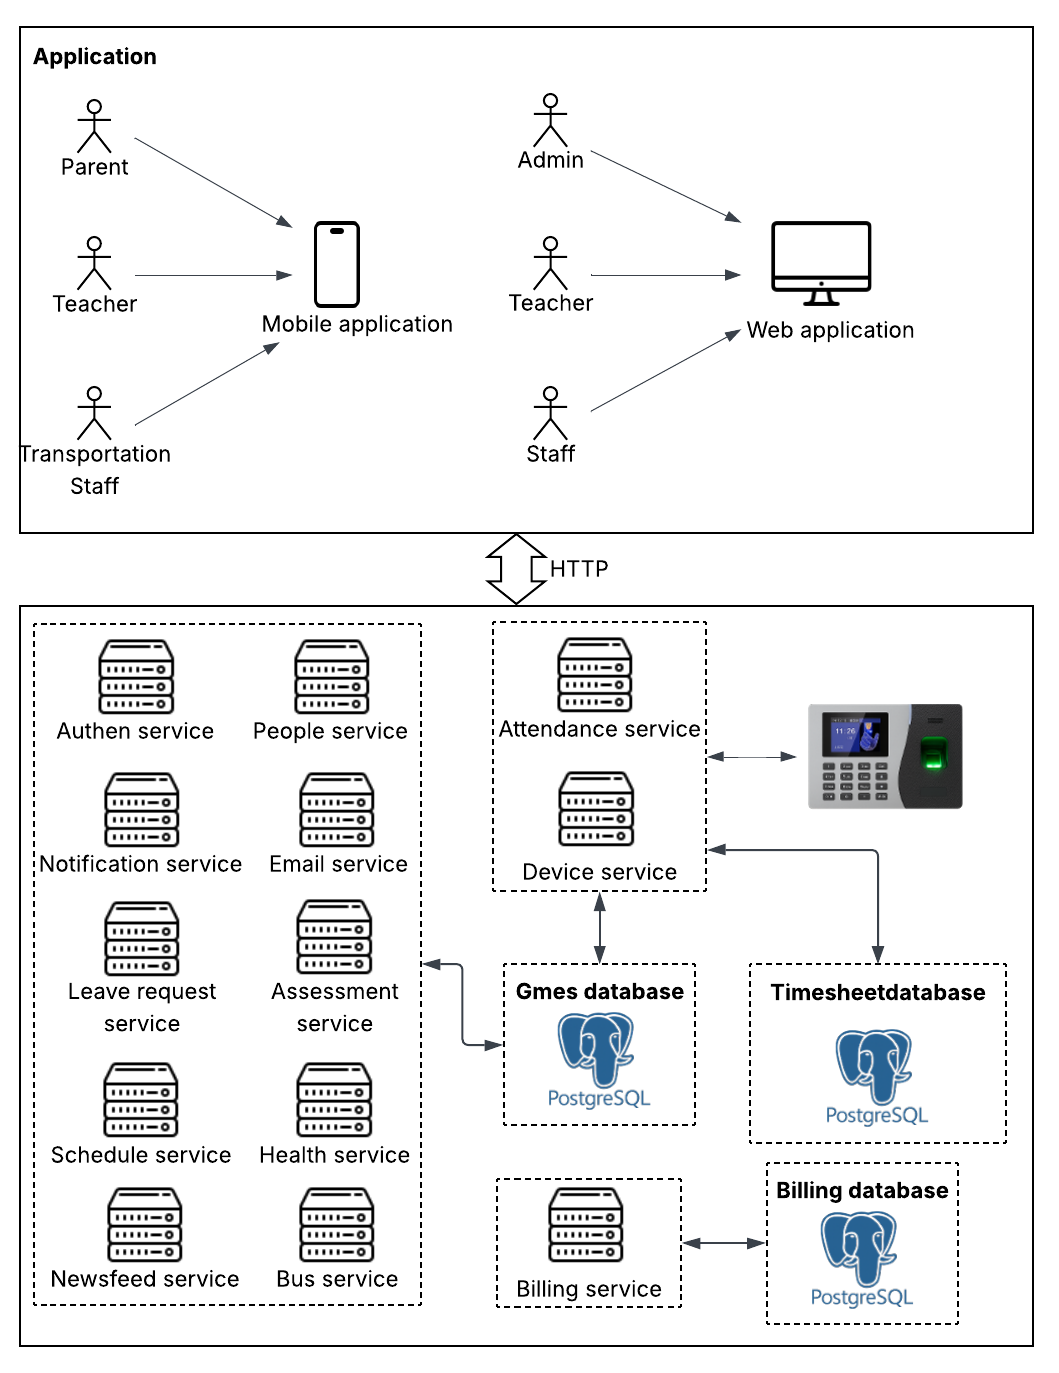
\includegraphics[width=0.9\textwidth]{images/sad_overview.png}
    \vspace{-1em}
    \caption{System architecture overview.}
    \label{fig:system_architecture_diagram_overview}
\end{figure}
\begin{minipage}{\textwidth}
    \setlength{\parindent}{2em}
   As shown in \textbf{\autoref{fig:system_architecture_diagram_overview}} the comprehensive overview of system architecture, the system provides both web and mobile application for differences user roles. These apps communicate with the server using the HTTP protocol, ensuring secure and reliable data exchange.

   Since GMES School is a comprehensive system handling multiple complex operations, it is designed using a microservices architecture. This approach allows each service to be developed, deployed, and scaled independently.
   
   Furthermore, to mange and stored data for these services, three separate PostgreSQL relational databases is designed:
\end{minipage}\\
\vspace{-0.8em}
\begin{itemize}
\setlength{\itemsep}{-0.1cm}
    \item A \textbf{GMES database} for core school data
    \item A \textbf{Timesheet database} for attendance data
    \item A \textbf{Billing database} for financial operations
\end{itemize}

\vspace{-0.5em}
\indent Futhermore, the system also integrates with physical attendance machines to accurately record  employee check-ins and check-outs time.


    % 3.2 Software block diagram
  \subsection{Software Block Diagram}
  % WEB APPLICATION
\subsubsection{Web Application}
\vspace{-2em}
\begin{figure}[H]
    \centering
    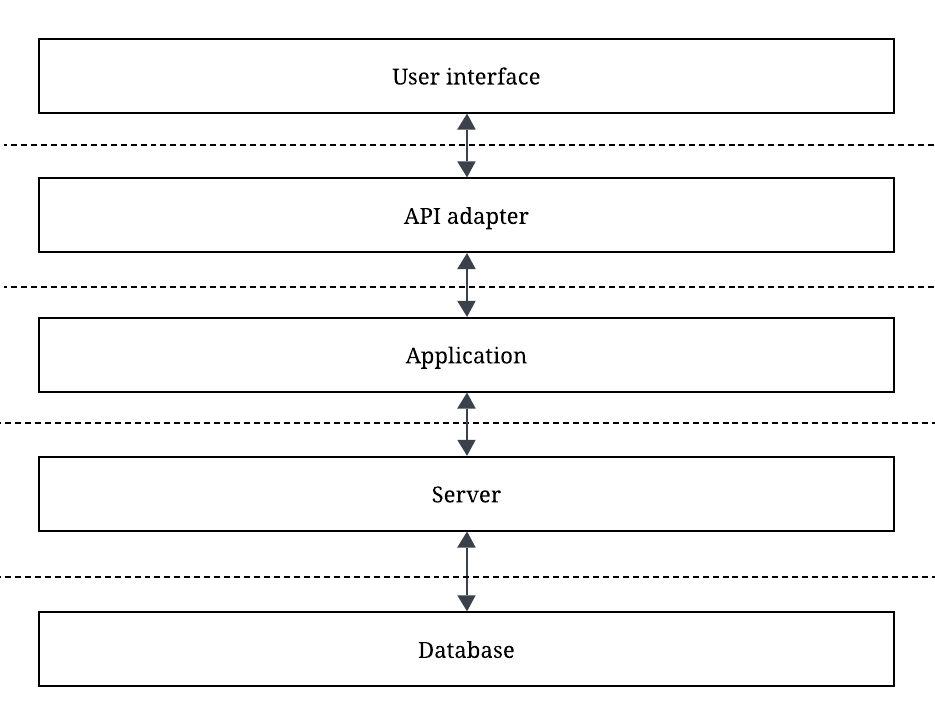
\includegraphics[width=1\textwidth]{images/bld_web_application.png}
    \vspace{-2em}
    \caption{Block Diagram of the Web application.}
    \label{fig:block_diagram_web}
\end{figure}
\begin{minipage}{\textwidth}
    \setlength{\parindent}{2em}
    \textbf{\autoref{fig:block_diagram_web}} above illustrates the high-level block diagram of the GMES School \textbf{web application system}. The architecture follows a layered approach where users interact with the system through the \textbf{User Interface} layer at the top. User requests are channeled through the \textbf{API Adapter}, which serves as the communication bridge between the frontend and backend services. These requests are processed by core services in the \textbf{Application layer}, which contains the business logic and application-specific functionality. The \textbf{Server layer} provides the runtime environment and infrastructure support, managing system resources, HTTP protocols, STOMP protocols, and service deployment. Finally, all processed data is stored and retrieved from the \textbf{Database layer}, which ensures data persistence, integrity, and security across the entire system.
\end{minipage}\\

\setlength{\parindent}{2em}Additionally, the system implements role-based access control, so that the application layer will provide different services and features based on the user's role.
% EMPLOYEE
\vspace{-0.4cm}
\begin{figure}[H]
    \centering
    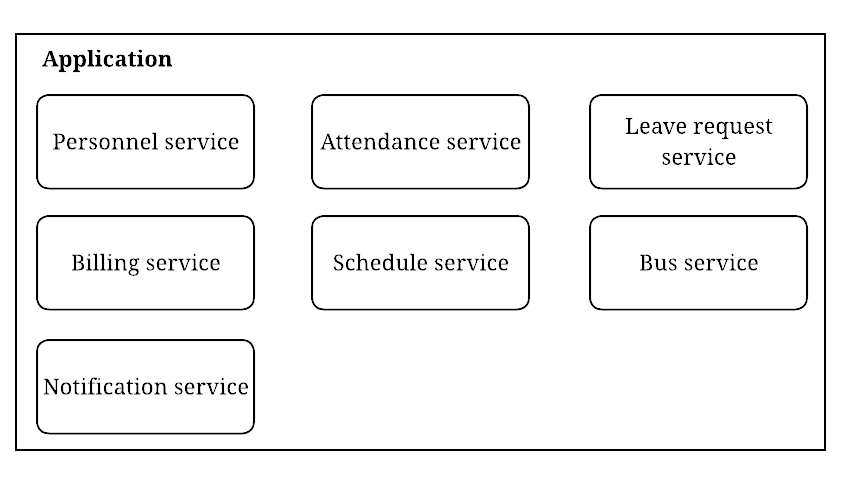
\includegraphics[width=0.8\textwidth]{images/bld_employee_web.png}
    \vspace{-1em}
    \caption{Application layer of the Web application for employees.}
    \label{fig:block_diagram_employee_web}
\end{figure}
\vspace{-0.4cm}
\setlength{\parindent}{2em} For \textbf{employees} (teachers and staff), the system provides several services illustrated in \textbf{\autoref{fig:block_diagram_employee_web}} that allow them to manage personnel records, attendance tracking, leave requests, salary processing, fee, scheduling, bus transportation, and notification.

% ADMIN
\vspace{-0.4cm}
\begin{figure}[H]
    \centering
    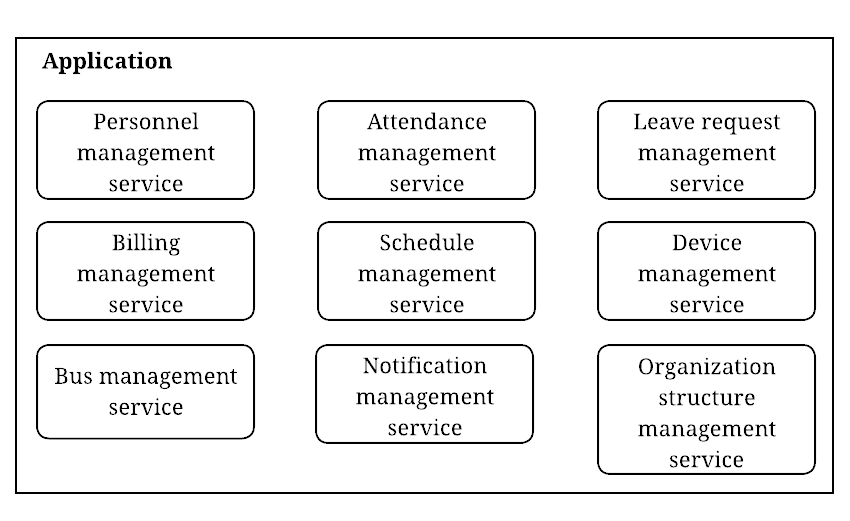
\includegraphics[width=0.8\textwidth]{images/bld_admin_web.png}
    \vspace{-1em}
    \caption{Application layer of the Web application for administrators.}
    \label{fig:block_diagram_admin_web}
\end{figure}
\vspace{-0.4cm}
\setlength{\parindent}{2em} For \textbf{administrators}, they have full access to all services that illustrated in \textbf{\autoref{fig:block_diagram_admin_web}}, complete oversight and control over all school operations through a unified platform.

% \setlength{\parindent}{2em}However, the functionality of these services will be hidden or provided based on the user's type and assigned role. This ensures that employees only access features relevant to their responsibilities and authorization level.


%MOBILE APP
\subsubsection{Mobile Application}
\begin{minipage}{\textwidth}
    \setlength{\parindent}{2em}
    The mobile application's architecture follows the same layered approach as the web application, as illustrated in \textbf{\autoref{fig:block_diagram_web}}.
\end{minipage}\\[0.17cm]
\indent Currently, the system's mobile application supports only three types of users: parents, teachers, and transportation staff. Therefore, the application layer provides different services and features based on the user type.
%TEACHER
\vspace{-0.7cm}
\begin{figure}[H]
    \centering
    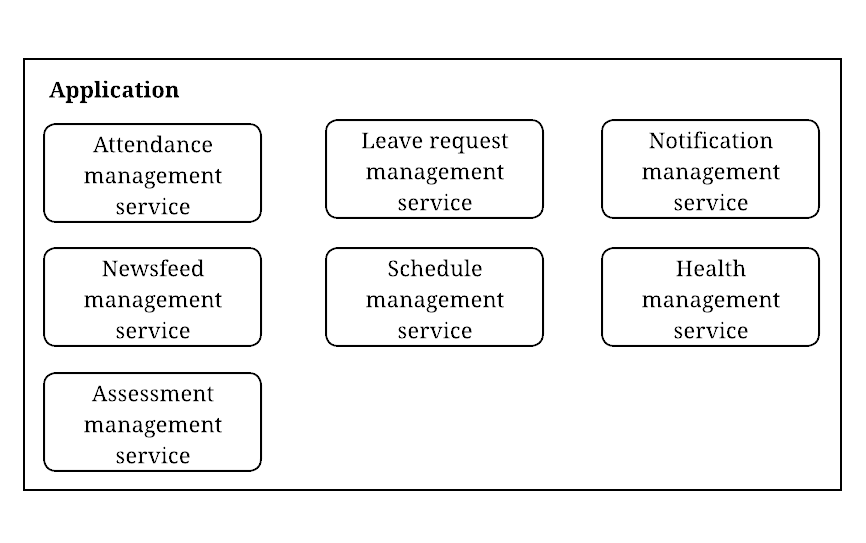
\includegraphics[width=0.8\textwidth]{images/bld_teacher_mobile_app.png}
    \vspace{-2em}
    \caption{Application layer of the Mobile Application for teachers.}
    \label{fig:block_diagram_teacher_mobile_app}
\end{figure}
\vspace{-0.4cm}
\setlength{\parindent}{2em}For \textbf{teachers}, the application layer integrates seven core services, as illustrated in \textbf{\autoref{fig:block_diagram_teacher_mobile_app}}, covering attendance, leave request, notifications, newsfeed, scheduling, health, and assessments. These integration services eliminate manual paperwork and time-consuming processes, help efficiently manage student-related activities, and maintain better communication with parents.
% PARENT MOBILE
\vspace{-0.7cm}
\begin{figure}[H]
    \centering
    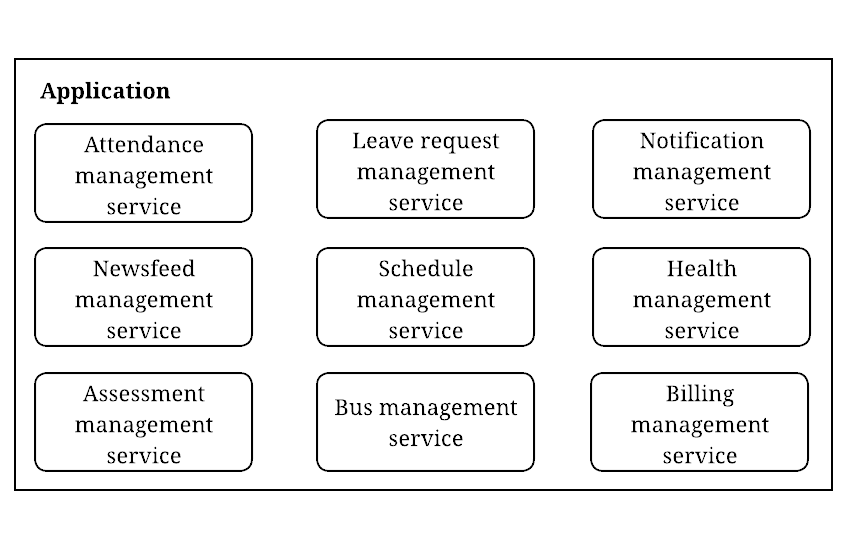
\includegraphics[width=0.8\textwidth]{images/bld_parent_mobile_app.png}
    \vspace{-2em}
    \caption{Application layer of the Mobile Application for parent.}
    \label{fig:block_diagram_parent_mobile_app}
\end{figure}
\vspace{-0.4cm}
\setlength{\parindent}{2em}For \textbf{parents}, the application layer provides several services, as illustrated in \textbf{\autoref{fig:block_diagram_parent_mobile_app}} that allow them to manage all aspects related to their children at school. By integrating these services into a single, user-friendly application, parents can gain greater control and convenience in supporting their children’s education.

% BUS MANAGER MOBILE APP
\begin{figure}[H]
    \centering
    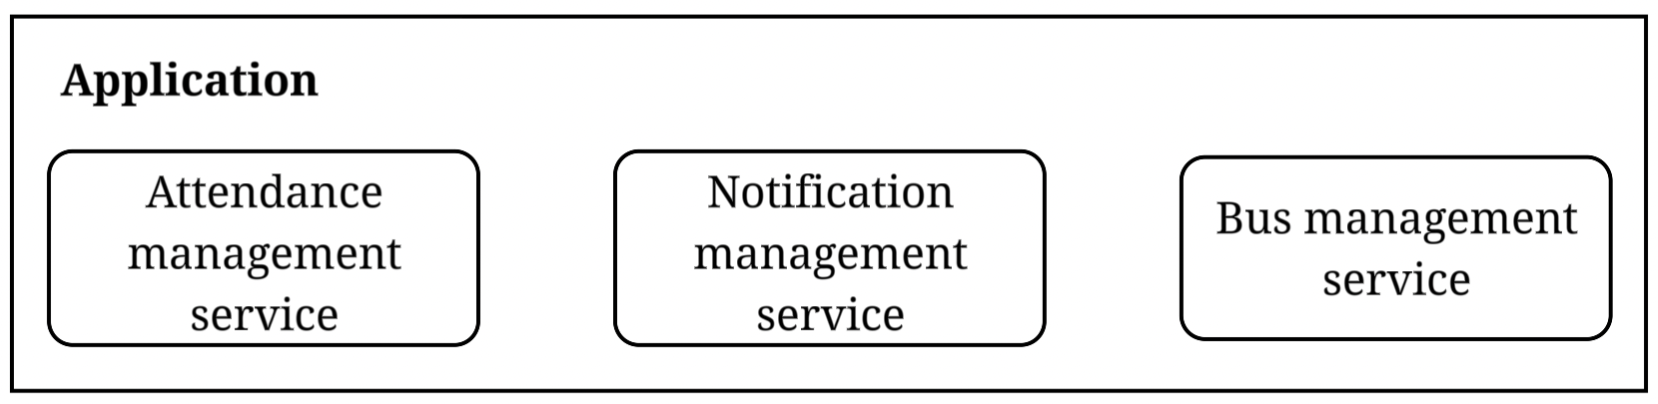
\includegraphics[width=0.8\textwidth]{images/bld_bus_manager_mobile_app.png}
    \vspace{-0.2em}
    \caption{Application layer of the Mobile Application for transportation staff.}
    \label{fig:block_diagram_bus_manager_mobile_app}
\end{figure}
\vspace{-0.4cm}
\setlength{\parindent}{2em}For \textbf{transportation staff}, the application provides only three services, as illustrated in \textbf{\autoref{fig:block_diagram_bus_manager_mobile_app}}. These services enable bus managers to efficiently manage bus routes, notifications and monitor student attendance during transportation.

  % 3.3 Database design
  \subsection{Database Design}
  % \begin{minipage}{\textwidth}
    \setlength{\parindent}{2em}
    Following the analysis of the system requirements, this section outlines the \textbf{database tables supporting the modules and features under my responsibility}. It provides both a high-level overview and detailed descriptions of the entities, their attributes, and their relationships.
\end{minipage}


\subsubsection{Extracted database tables}
\noindent
\begin{minipage}{\textwidth}
    \setlength{\parindent}{2em}
    This part illustrated the \textbf{high-level overview of the extracted database tables for modules and features under my responsibility} through the Entity-Relationship Diagram (ERD). The ERD visually represents the core entities, their attributes, and the relationships between them.
\end{minipage}
\begin{figure}[H]
    \centering
    % 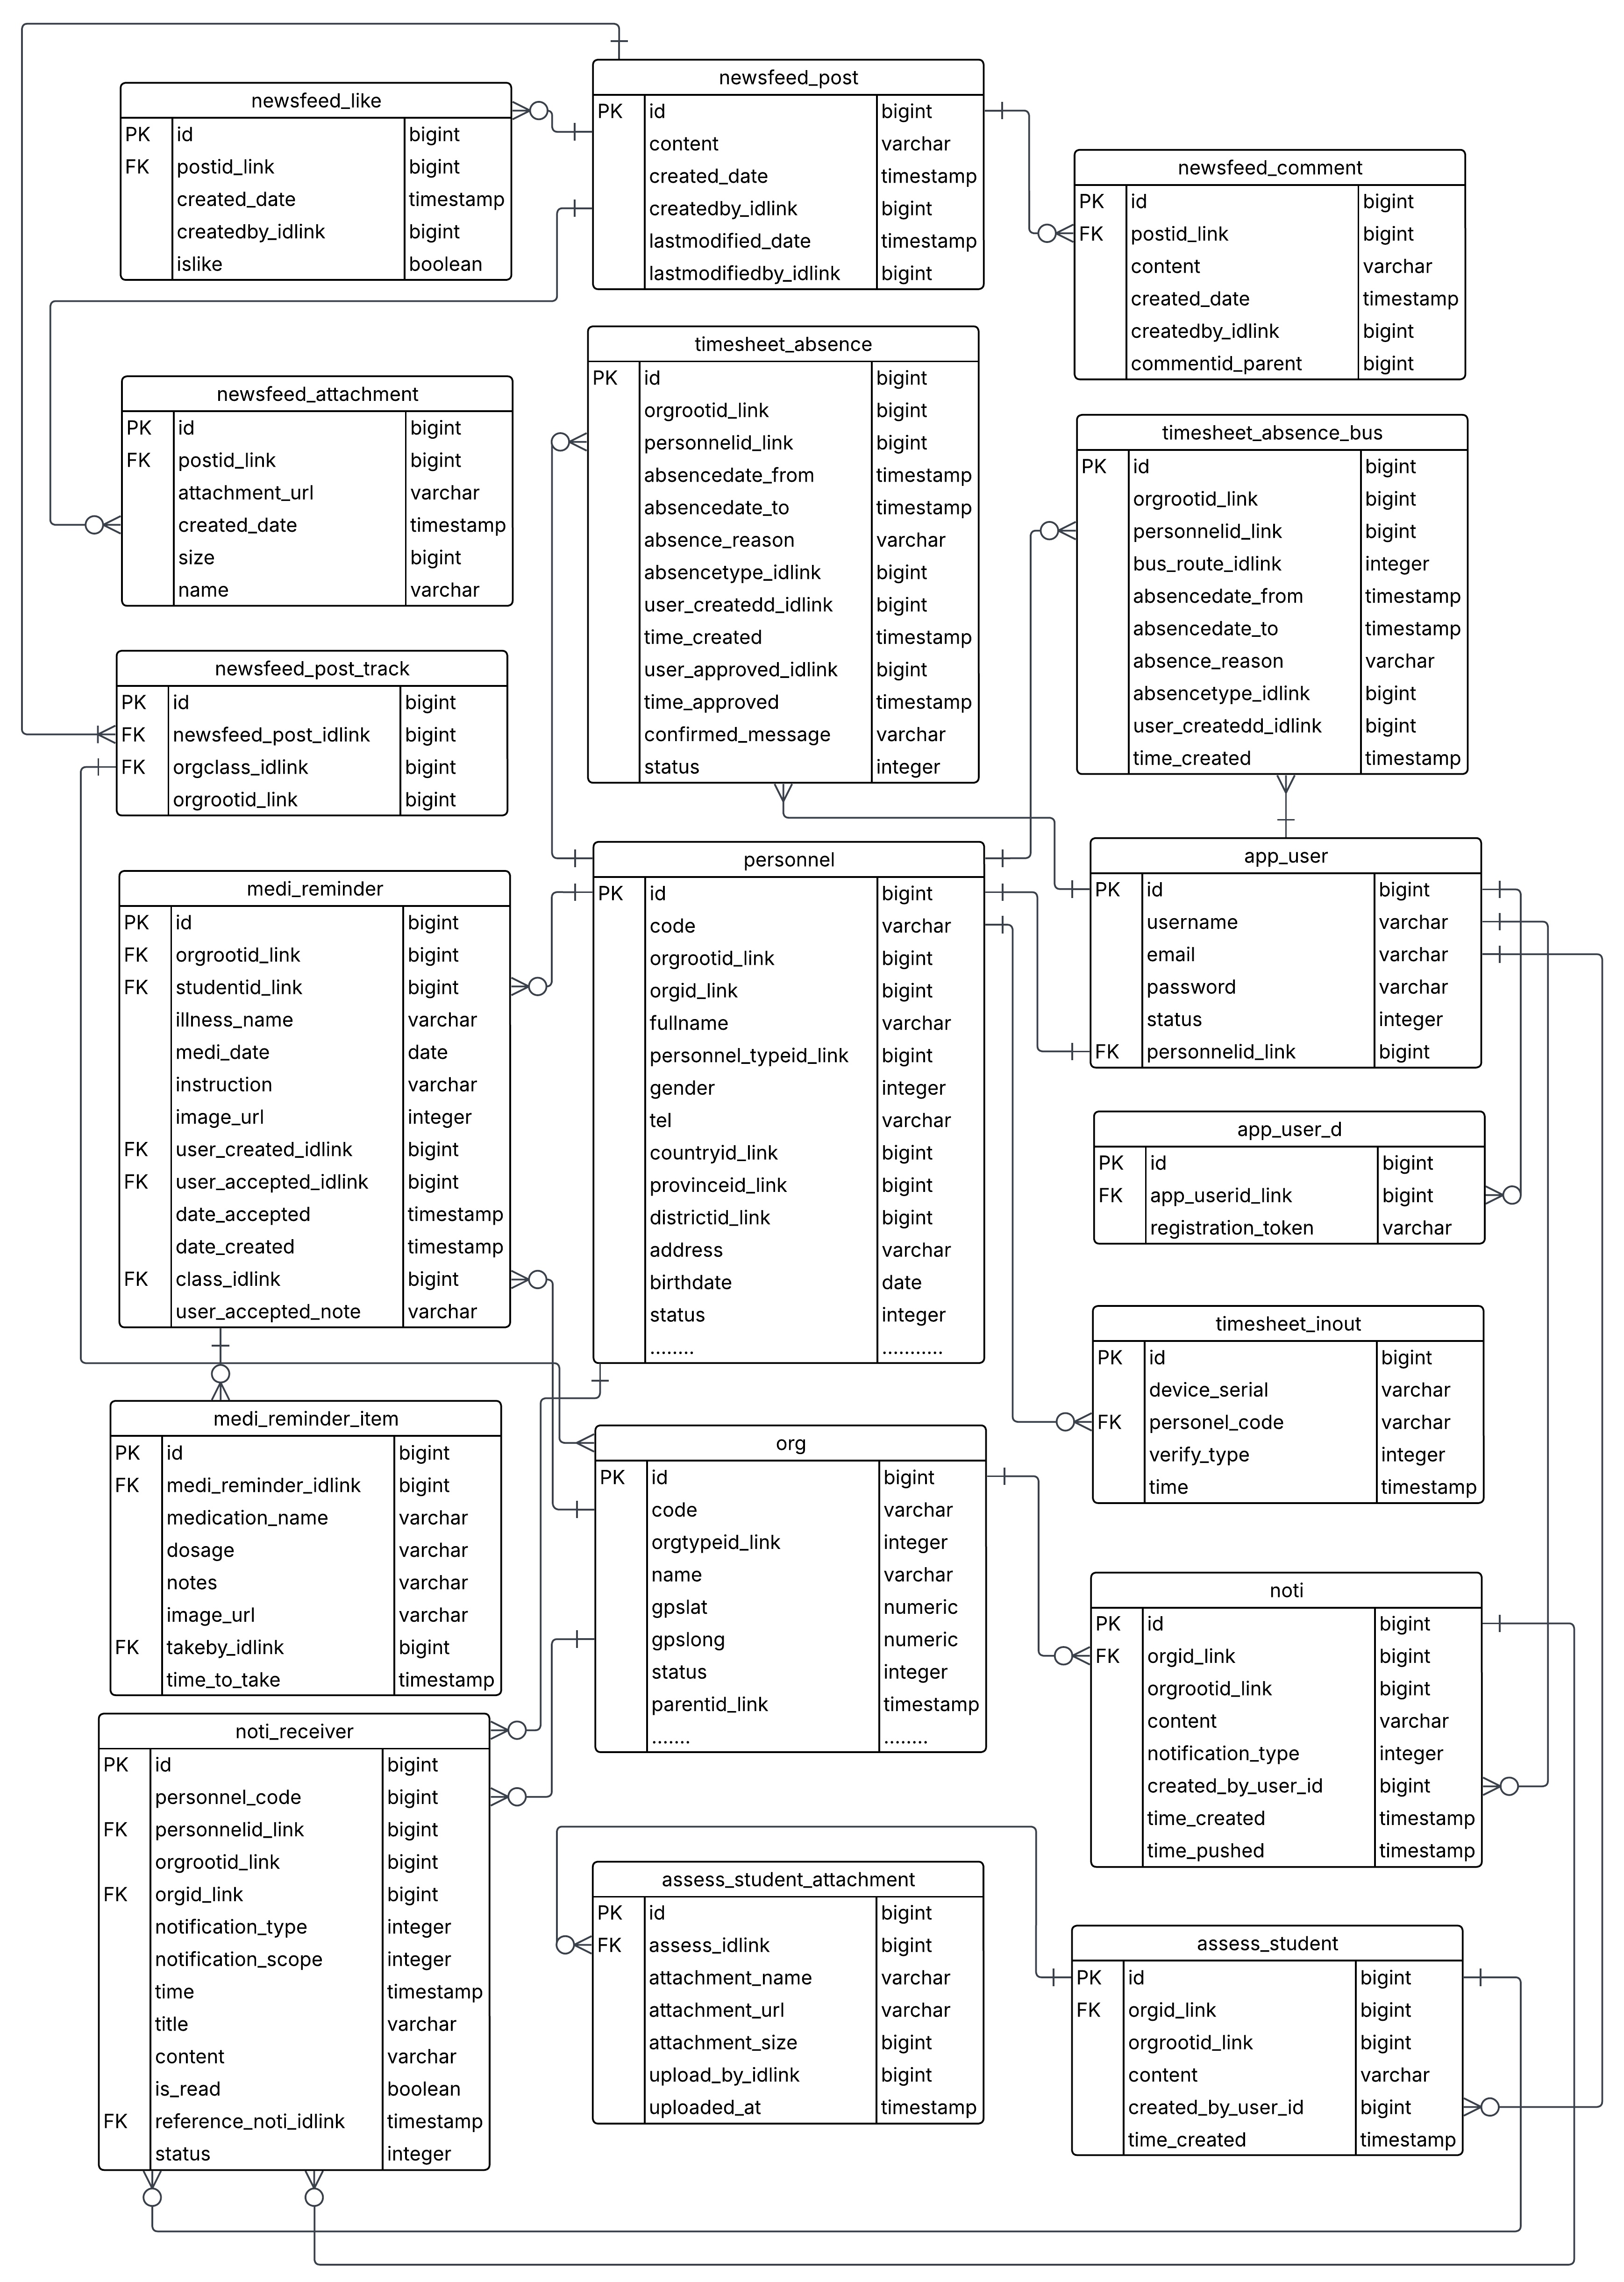
\includegraphics[width=1.05\textwidth]{images/database_erd.png}
    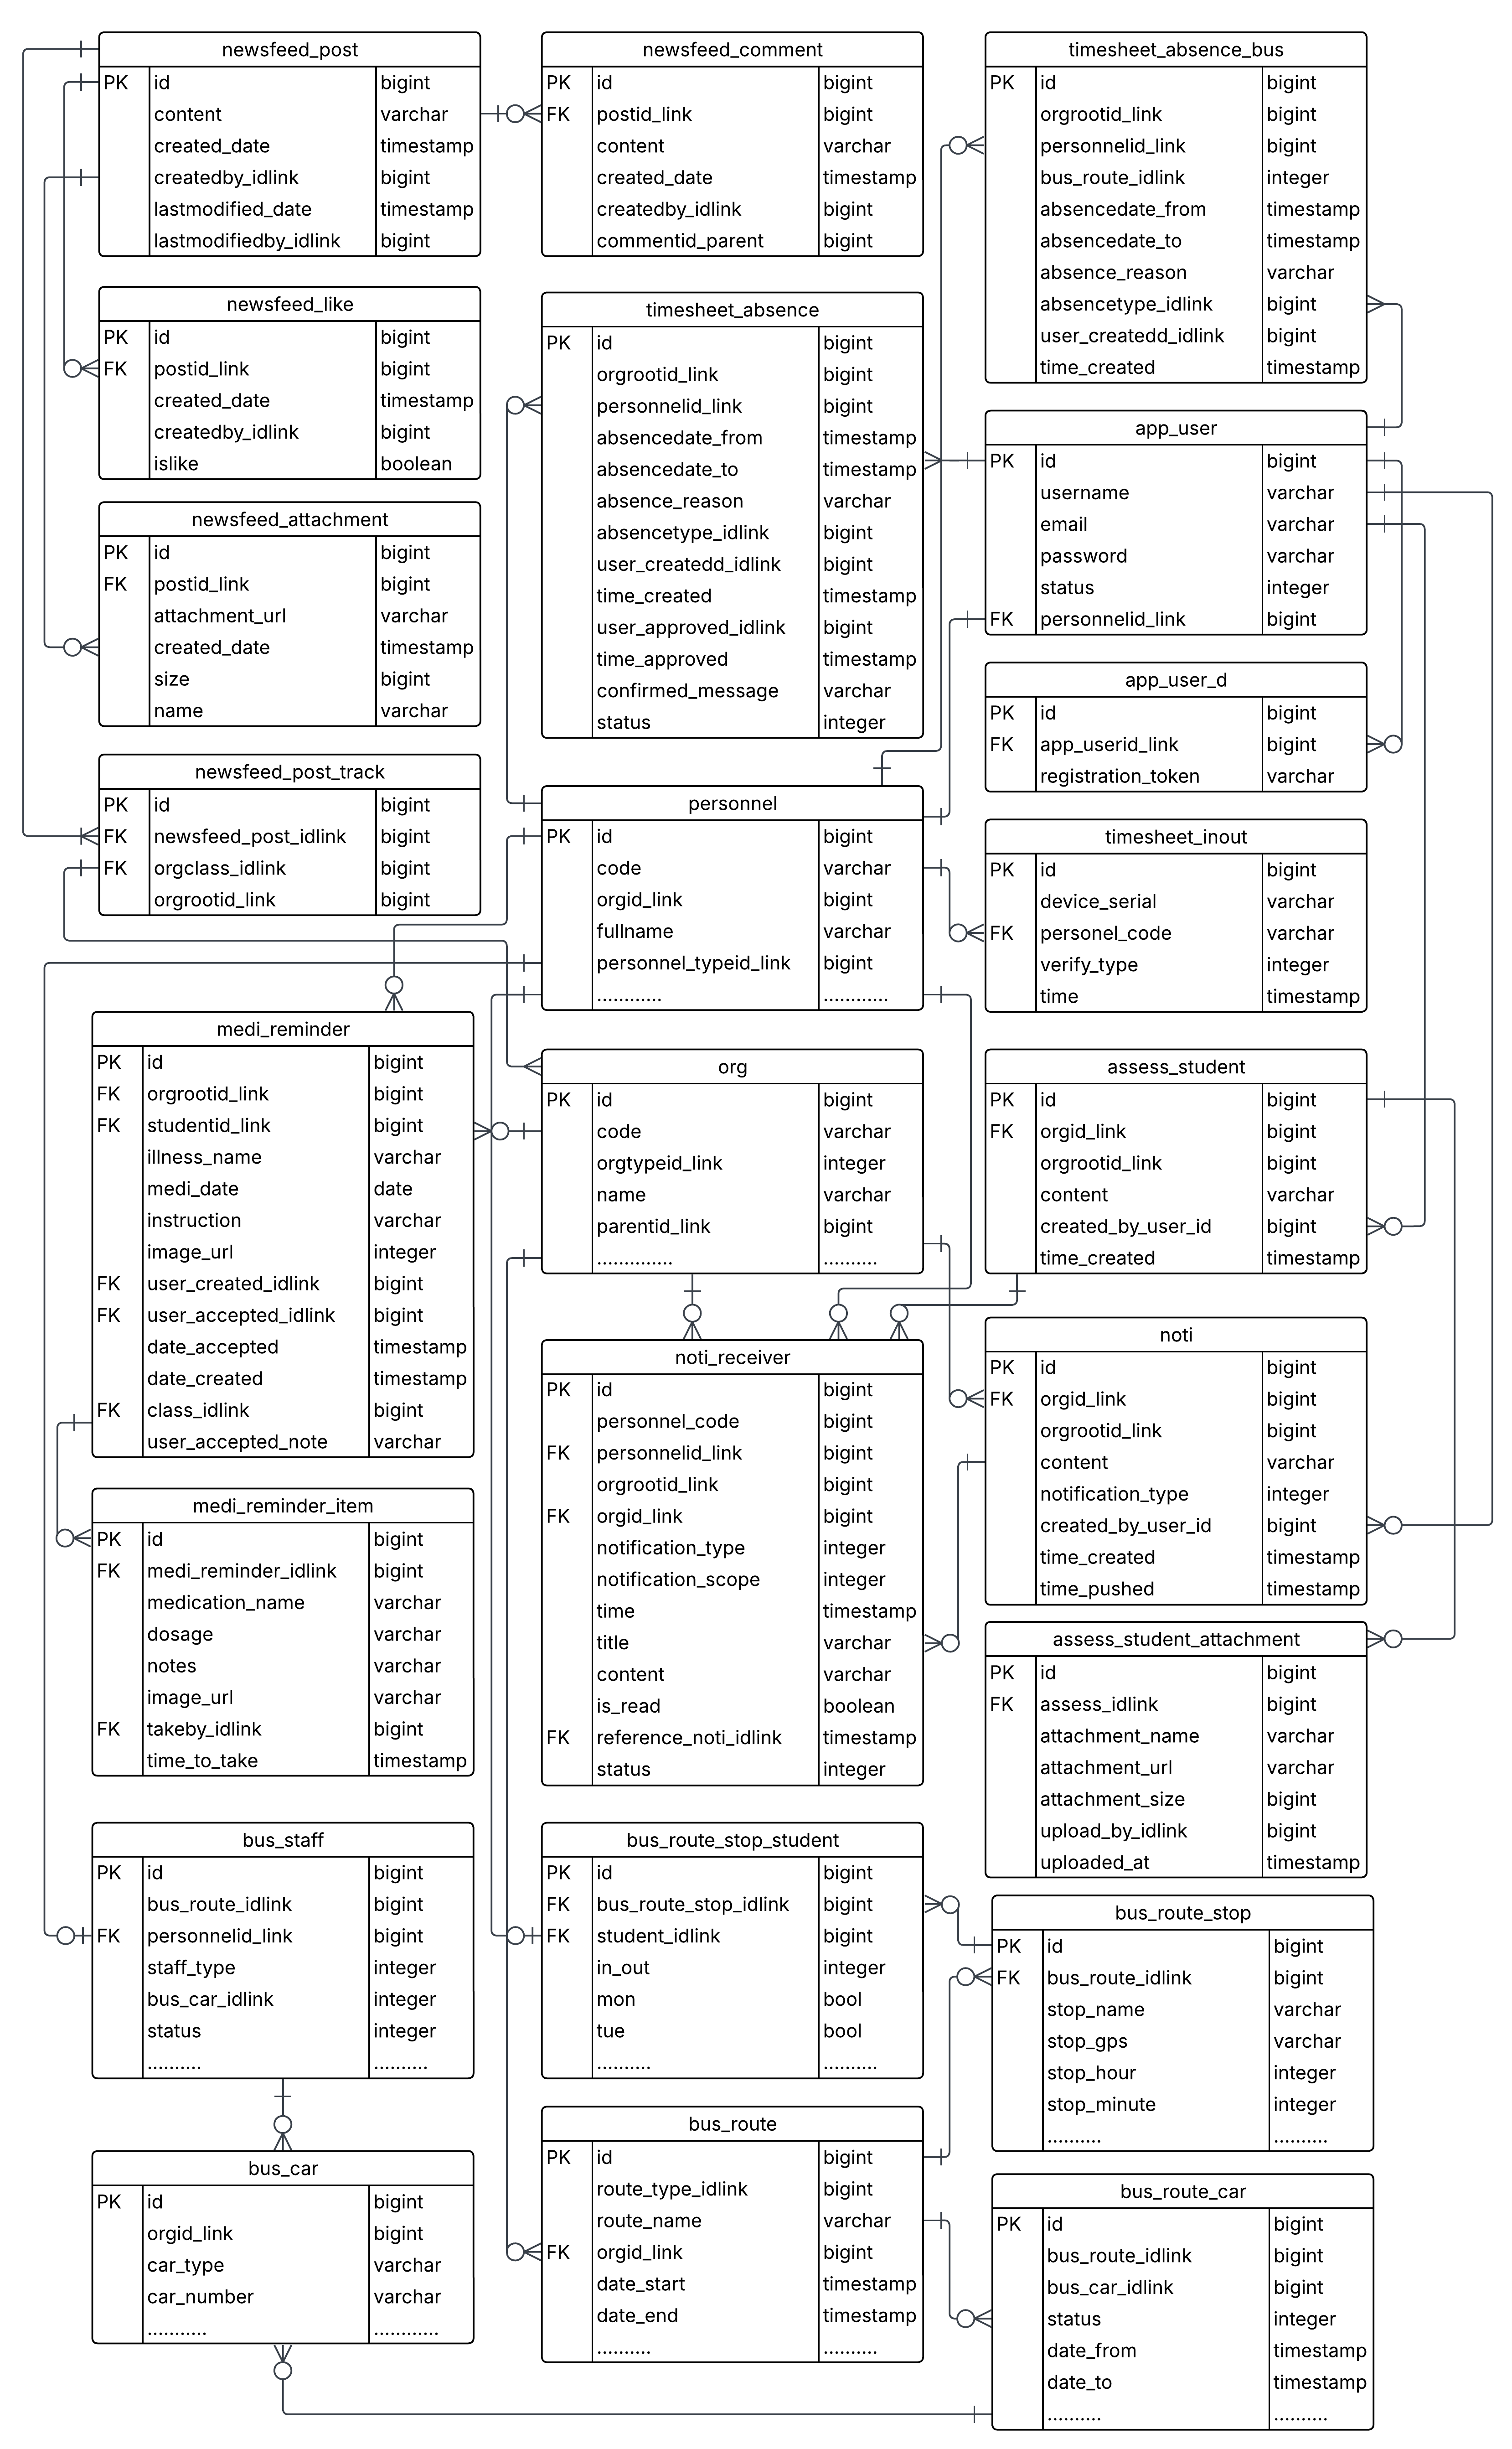
\includegraphics[width=1\textwidth]{images/image.png}
    \caption{Extracted database tables.}
    \label{fig:database_erd}
\end{figure}

\subsubsection{Database Design Description}
\noindent
\begin{minipage}{\textwidth}
    \setlength{\parindent}{2em}
    This section explain the \textbf{Extracted database tables} illustrated in \textbf{\autoref{fig:database_erd}} that related to the \textbf{features and modules assigned to me} in this project. Below is a detailed description of each entity and the relationships between them.
    % In this section, we will explain the Entity-Relationship Diagram (ERD) illustrated in \textbf{\autoref{fig:database_erd}} by describing each entity and its attributes, the relationships and cardinalities between entities, and how this design supports the system requirements.
\end{minipage}
\vspace{-0.8em}
\begin{itemize}[itemsep=-0.1cm]
    \item \textbf{personnel}: The table stores detailed information about both employees and students, which can be identified using the personnel\_typeid\_link attribute. It includes basic personal details (name, gender, birth date, contact, status) along with additional data specific to students and employees. This design ensures efficient management of personal information.
    \item \textbf{org}: The org table stores information about all organizational units (schools, departments, classes, etc) and uses the parentid\_link attribute to maintain a hierarchical structure.
    \item \textbf{app\_user}: This table stores user login credentials and controls access to the system. For security purposes, all passwords are encrypted using the Bcrypt hashing algorithm.
    \item \textbf{app\_user\_d}: The table manages mobile device access by linking each device token to a user account. These tokens are then used to send notifications.
    \item \textbf{timesheet\_inout}: The table is used to record raw attendance data. It tracks which device was used (device\_serial), the verification method: face recognition, fingerprint, or manual entry by a teacher (verify\_type), and the time when attendance was recorded.
    \item \textbf{timesheet\_absence}: Stores leave requests for employees and students. It records the absence dates, reason, leave type, and tracks the complete approval process including who submitted it, when it was created, who approved it, and approval time.
    \item \textbf{timesheet\_absence\_bus}: The table is used to track bus leave requests when students request time off from bus service, ensuring coordination between attendance and transportation management.
    \item \textbf{newsfeed\_post}: The main table for storing newsfeed content. Each post can be associated with multiple related entities, including newsfeed likes, comments, and attachments, enabling scalability.
    \item \textbf{newsfeed\_attachment}: The table manages attachments associated with newsfeed posts using URLs. It stores metadata like file name, size, and creation time, while the actual files are stored on the server and referenced by URLs.
    \item \textbf{newsfeed\_like}: The table manages user reactions to newsfeed posts, tracking which users have interacted with specific posts.
    \item \textbf{newsfeed\_comment}: The table manages user comments on newsfeed posts. It tracks who commented, the content, and timestamp while supporting hierarchical reply structures through the commentid\_parent field.
    \item \textbf{medi\_reminder}: The table stores the medicine reminders for students. It captures illness details, medication dates, treatment instructions, and tracks who created the reminder and which teacher confirmed it.
    \item \textbf{medi\_reminder\_item}: The table stores individual medicine details within each reminder request. These records maintain a direct relationship with their corresponding medication reminders through the medi\_reminder\_idlink.
    \item \textbf{assess\_student}: The assess\_student manages assessments for individual or multiple students.
    \item \textbf{assess\_student\_attachment}: The table manages file attachments associated with assessments using URLs. It stores metadata like file name, size, and creation time.
    \item \textbf{noti}: The table stores notifications to be pushed to users. Each record contains content, title, scope (whole organization, school, or class level), and type (attendance, leave requests, medicine reminders, etc.)
    \item \textbf{noti\_receiver}: The table tracks notifications or assessments sent to individual users. It records who received it, when it was sent, read status, and delivery status.
    \item \textbf{bus\_route}: The table is designed to store and manage information about bus routes. Its primary purpose is to track details such as route names, assigned vehicles, drivers, managers, and operational schedules, ensuring efficient organization and monitoring of bus routes.
    \item \textbf{bus\_route\_stop}: The table designed to store individual pickup and drop-off points  within a bus route. It define the sequential priority, timing, and location of stops, ensuring accurate scheduling and reliable navigation for both transportation staff and students.
    \item \textbf{bus\_route\_stop\_student}: The table links students to specific bus routes and stops, helping the system track assignments and improve bus operation efficiency and safety.
    \item \textbf{bus\_route\_staff}: The table assigns transportation staff (drivers, managers) to bus routes, allowing flexible allocation of drivers and managers to different routes as needed.
    \item \textbf{bus\_route\_car}: This table links buses to routes over time, allowing flexible assignments and preventing scheduling conflicts across the transportation network.
    \item \textbf{bus\_car}: The table stores detailed information about all school buses including vehicle type, license plate, description, and seating capacity. This centralized registry enables efficient assignment of specific buses to designated routes, ensuring optimal fleet utilization and proper matching of vehicle capacity to route requirements.
\end{itemize}


% IV. METHODOLOGY
\newpage
\section{METHODOLOGY}\label{sec:methodology}
  \indent

  This section details the methodologies used to develop the modules and features assigned to me. It explains why each approach was chosen and shows how these approaches helped solve the problems.
  % 4.1
  % \subsection{Technologies}
  % SENCHA EXT JS
\subsection{Sencha Ext JS}
\begin{minipage}{\textwidth}
    \setlength{\parindent}{2em}
    Sencha Ext JS is a comprehensive JavaScript framework for building data-intensive, cross-platform web applications. It is used for UI development \textbf{due to several reasons}: its \textbf{rich component library}, support for the \textbf{MVC architecture}, \textbf{responsive and cross-browser} compatibility, and \textbf{high performance}.
\end{minipage}\\

% FLUTTER
\subsection{Flutter}
\begin{minipage}{\textwidth}
    \setlength{\parindent}{2em}
    Flutter is an open-source mobile application development framework created by Google. It is chose to develop the GMES School mobile application \textbf{because of} several reasons:
\end{minipage}
\begin{itemize}
\setlength{\itemsep}{0.0em}
    \item \textbf{Cross-platform Development}: A single codebase that can create applications for both iOS and Android, helping save development time and ensuring consistency in user experience across platforms.
    \item \textbf{Widget-based Architecture}: I can built the interface by combining various widgets such as ListView for displaying data lists, Card widgets for information presentation, and custom widgets for specific functionalities throughout the application.
    \item \textbf{State Management}: Implemented GetX state management to manage the application state, ensuring data synchronization across different screens.
\end{itemize}

% SPRING
\subsection{Spring boot}
\begin{minipage}{\textwidth}
    \setlength{\parindent}{2em}
    Spring Boot is a Java framework that is used to build the GMES School system, allowing me to develop the backend, RESTful APIs, and real-time communication using STOMP over WebSocket quickly and efficiently. It is chosen because of its \textbf{integration with the Spring ecosystem} (including Dependency Injection and Spring Security), support for \textbf{auto-configuration} to speed up development, \textbf{microservices architecture} for scalable services, and its \textbf{built-in Tomcat server} for easy deployment to our VPS.
\end{minipage}\\

% POSTGRE SQL
\subsection{PostgreSQL}
\begin{minipage}{\textwidth}
    \setlength{\parindent}{2em}
    PostgreSQL is a powerful, open-source relational database management system (RDBMS) used to manage and process data. PostgreSQL is selected for the GMES School project due to its \textbf{superior performance} and \textbf{reliability}, especially when compared to alternatives like MySQL. As GMES School manages multiple institutions and thousands of users within a microservice architecture, PostgreSQL efficiently handles \textbf{high-concurrency workloads} with minimal delay. Additionally, \textbf{its accurate decimal arithmetic} ensures precise financial calculations, making it essential for maintaining system integrity and performance.
\end{minipage}\\

% OBJECT-RELATIONAL MAPPING
\subsection{Object-Relational Mapping}
\indent\indent The system implemented Hibernate ORM as the persistence layer framework to facilitate the interaction between the GMES Java application and the PostgreSQL database. ORM serves as a crucial bridge that maps object-oriented programming concepts to relational database structures, allowing me to focus on core educational management features instead of low-level database operations.

% PAGINATION
\subsection{Pagination}
\begin{minipage}{\textwidth}
    \setlength{\parindent}{2em}
    The GMES School system manages large datasets across multiple educational institutions, including comprehensive employee and student records. To maintain performance and user experience, I use pagination to \textbf{retrieve data in smaller chunks} instead of loading entire datasets at once.
\end{minipage}\\


% FIREBASE CLOUD MESSAGING
\subsection{Firebase Messaging Cloud}
\begin{minipage}{\textwidth}
    \setlength{\parindent}{2em} Push notifications are essential to the system, keeping parents, teachers, and transportation staff informed of important updates. Therefore, the system integrates Firebase Cloud Messaging (FCM) as its push notification solution due to its \textbf{reliability}, \textbf{cross-platform}, and scalable architecture that can \textbf{handle simultaneous notifications}.
\end{minipage}\\

% STOMP OVER WEBSOCKET
\subsection{STOMP Over WebSocket}
\begin{minipage}{\textwidth}
    \setlength{\parindent}{2em} In this project, I use STOMP over WebSocket to enable real-time bus tracking. WebSocket provides a persistent, full-duplex connection, while STOMP adds a structured messaging protocol that simplifies routing and processing. This combination allows Flutter mobile app and Spring Boot backend to exchange messages efficiently in real time. It enables key features such as:
\end{minipage}
\begin{itemize}[itemsep=-0.1cm, topsep=0.25cm]
    \item \textbf{Pub-Sub Messaging}: for broadcasting bus locations.
    \item \textbf{Targeted Messages}: to individual users
    \item \textbf{Acknowledgment Mechanisms}: for reliable delivery.
\end{itemize}



% V. TESTING
\newpage
\section{TESTING}\label{sec:testing}
  \indent

  This section outlines the systematic testing and evaluation procedures used to verify the functionality, and reliability of key features implemented in this project. The comprehensive testing approach ensures that each module operates correctly under various conditions and meets the established quality criteria.
  % 4.1
  % \subsection{Technologies}
  \renewcommand{\arraystretch}{1.2}
\begin{longtable}{|>{\raggedright\arraybackslash}p{3cm}|
                  >{\raggedright\arraybackslash}p{5cm}|
                  >{\raggedright\arraybackslash}p{5cm}|
                  >{\centering\arraybackslash}p{2cm}|}                  
\caption{System Functional Test Plan.}
\label{tab:test_plan} \\
\hline
\textbf{Test case} & \textbf{Steps} & \textbf{Expected Result} & \textbf{Status} \\
\hline
\endfirsthead
\endhead

Import employee data feature. & 
1. Navigate to Employee Profile → Import function.
\newline
2a. Upload valid Excel file with employee data.
\newline
2b. Upload invalid file (wrong format/missing columns).
\newline
2c. Upload file with duplicate employee codes, identities & 
1. Display user's managed departments in tree structure.
\newline
2a. Successfully import data, refresh employee list, show success message.
\newline
2b. Display specific error message (invalid format/missing required columns).
\newline
2c. Display error for duplicate entries, import only valid records. & 
PASS \\
\hline

Mark Student Attendance & 
1. Navigate to Attendance feature for selected class.
\newline
2. Mark students as present/absent/late.
\newline
3. Attempt to mark attendance for future dates.
\newline
4. Try to modify past attendance records.& 
1. Display student list with current attendance status.
\newline
2. Save attendance to database, send notifications to parents.
\newline
3. Future dates should be disabled in calendar.
\newline
4. Past records should be read-only.& 
PASS \\
\hline

Generate Student Attendance Report & 
1. Navigate to Student Attendance Report.
\newline
2. Select date range and generate report.
\newline
3. Export report to Excel format.
\newline
4. Try invalid date range. & 
1. Display departments managed by user.
\newline
2. Show attendance records with status indicators.
\newline
3. Download Excel file with formatted data.
\newline
4. Display validation error message. & 
PASS \\
\hline

Create Student Leave Requestt & 
1. Navigate to Leave Request feature.
\newline
2. Fill required fields and submit.
\newline
3. Create in leave request (overlapping, holiday conflicts, in valid date range). 
\newline
4. Submit request with missing mandatory fields or invalid field.& 
1. Display recent leave requests.
\newline
2. Save request, update student status, and send notification to teacher.
\newline
3. Display error message.
\newline
4. Disable submit button until all fields completed and valid.& 
PASS \\
\hline

Confirm Student Leave Request & 
1. Navigate to Confirm Leave request feature.
\newline
2. Review and approve/reject/revoke request.
\newline
3. Try to confirm expired leave request. & 
1. Display pending leave requests by priority.
\newline
2. Update request status, log approver info, and send notification to parents.
\newline
3. Show error for expired requests. & 
PASS \\
\hline

Post newsfeed & 
1. Navigate to Newsfeed feature.
\newline
2. Create post with text and images.
\newline
3. Upload attachments exceeding 100MB limit. 
\newline
4. Post with video content.& 
1. Display latest 10 newsfeed posts.
\newline
2. Save post, make visible to parents and teachers.
\newline
3. Display file size limit error. 
\newline
4. Successfully upload and display video content.& 
PASS \\
\hline

Confirm medicine reminder & 
1. Navigate to Medicine Reminder feature.
\newline
2. Confirm a valid reminder.
\newline
3. Try to confirm expired reminder. & 
1. Display latest 10 medicine reminders.
\newline
2. Update reminder status and send notification to parent.
\newline
3. Display error for expired reminders (usage date passed). & 
PASS \\
\hline

Real-time Bus Tracking & 
1. Navigate to Bus feature as parent.
\newline
2. Select bus route to track.
\newline
3. Transportation staff disables GPS.
\newline
4. No transportation staff assigned to route.& 
1. Display all active registered bus routes.
\newline
2. Establish WebSocket connection, receive real-time location updates every 50 meters.
\newline
3. Display GPS error message to parent.
\newline
4. Show "No staff assigned" error message.& 
PASS \\
\hline

\end{longtable}

% VI. RESULTS AND DISCUSSIONS 
\newpage
\section{RESULTS AND DISCUSSIONS}\label{sec:results_and_discussion}
  \indent

  This section outlines the features and modules I implemented, followed by the key challenges encountered during development.
  % 5.1 Results
  \subsection{Results}
  \begin{minipage}{\textwidth}
    \setlength{\parindent}{2em}
    This part summarizes the modules and features implemented by me (both front-end and back-end). Specifically, \textbf{I have implemented the following modules}:
\end{minipage}
\begin{itemize}[itemsep=-0.05cm, topsep=0.1cm]
    \item \textbf{Leave Request Management} (for mobile)
    %% Leave request parent
    \begin{figure}[H]
    \centering
    \begin{subfigure}{0.45\textwidth}
        \centering
        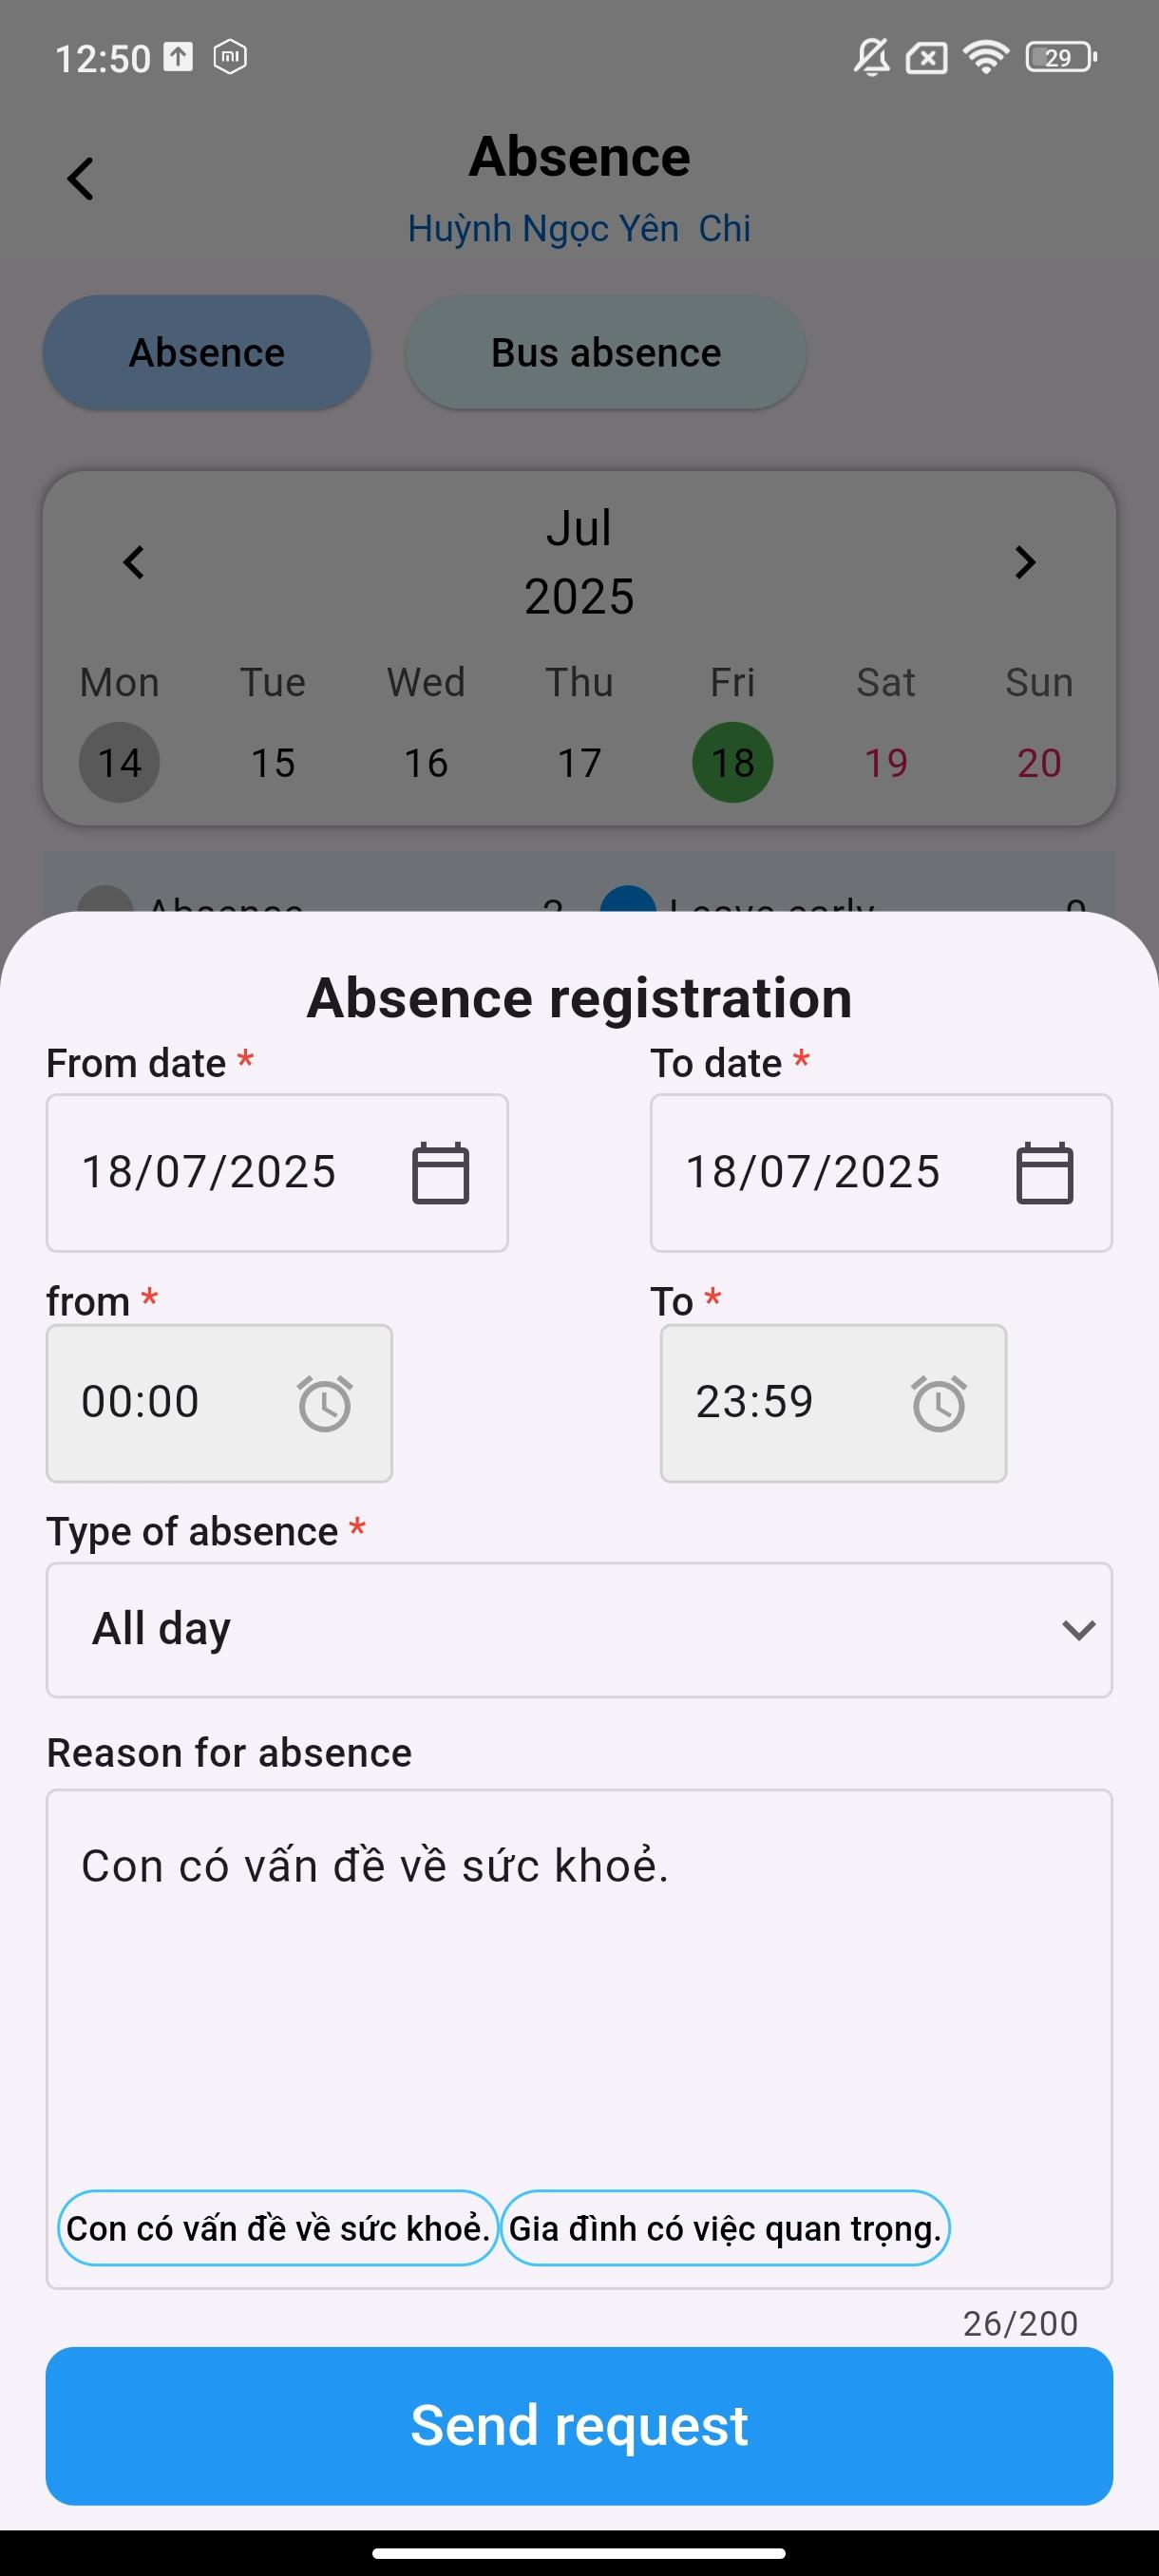
\includegraphics[width=0.6\textwidth]{images/create_leave_request_parent.png}
        \caption{Leave Request - Parent View}
        \label{subfig:leave_request_parent_view}
    \end{subfigure}
    \hfill
    \begin{subfigure}{0.45\textwidth}
        \centering
        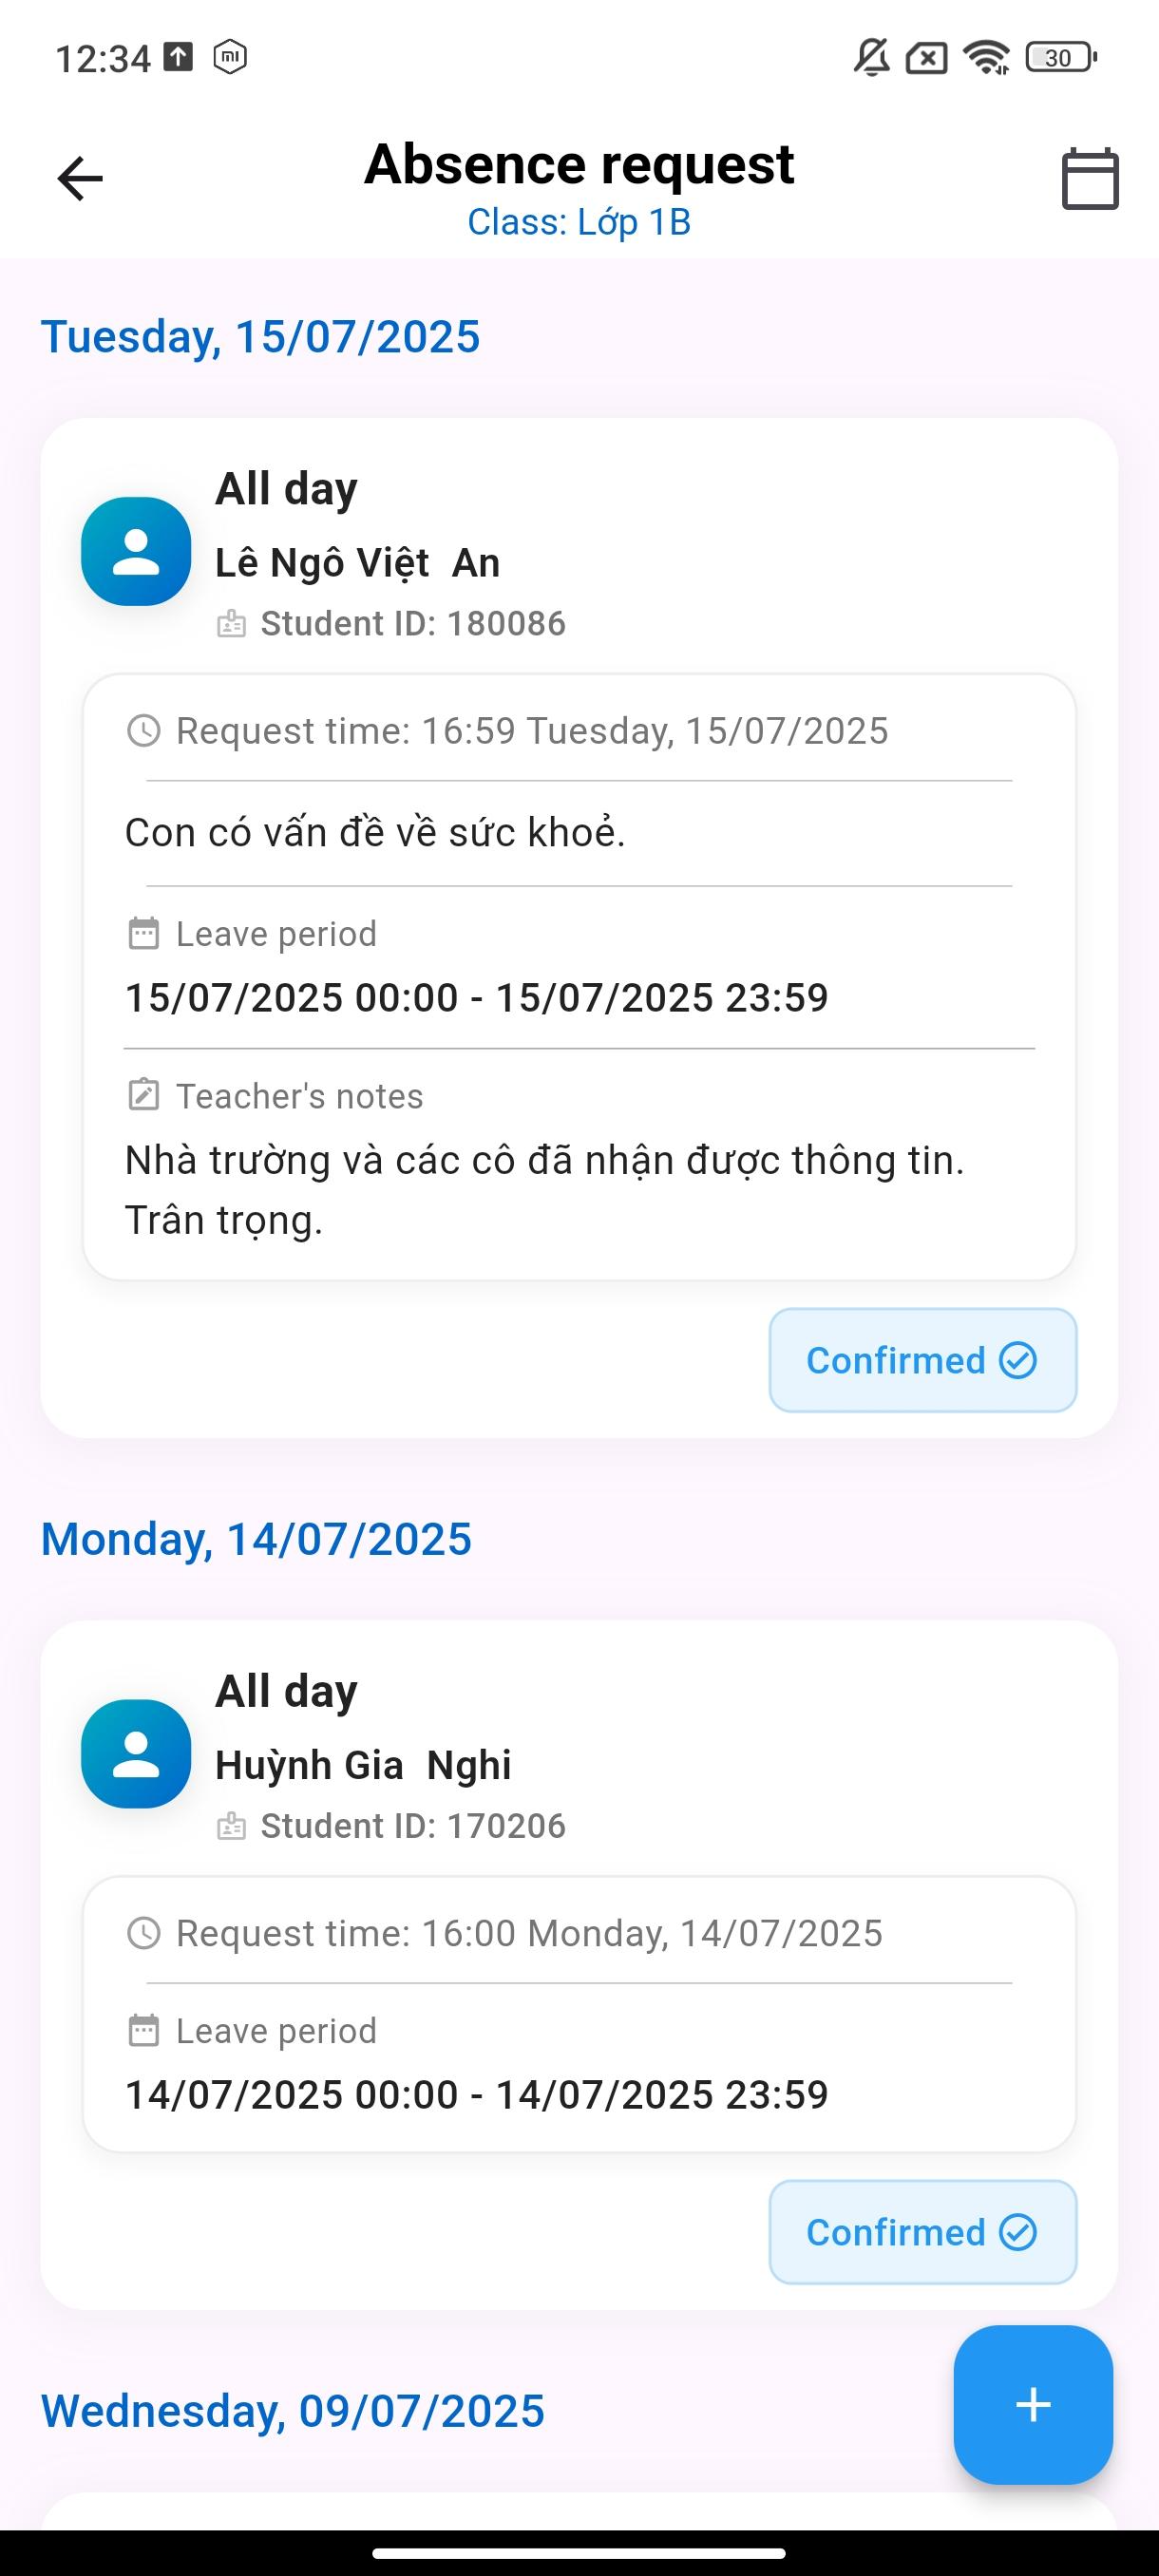
\includegraphics[width=0.6\textwidth]{images/approve_leave_request_teacher.png}
        \caption{Approve Leave - Teacher View}
        \label{subfig:create_leave_request_parent}
    \end{subfigure}
    \caption{Leave Request mobile app}
    \label{fig:leave_request_parent}
    \end{figure}
    %-------------------
    \newpage
    \item \textbf{Newsfeed Management}
    \begin{figure}[H]
    \centering
    \begin{subfigure}{0.45\textwidth}
        \centering
        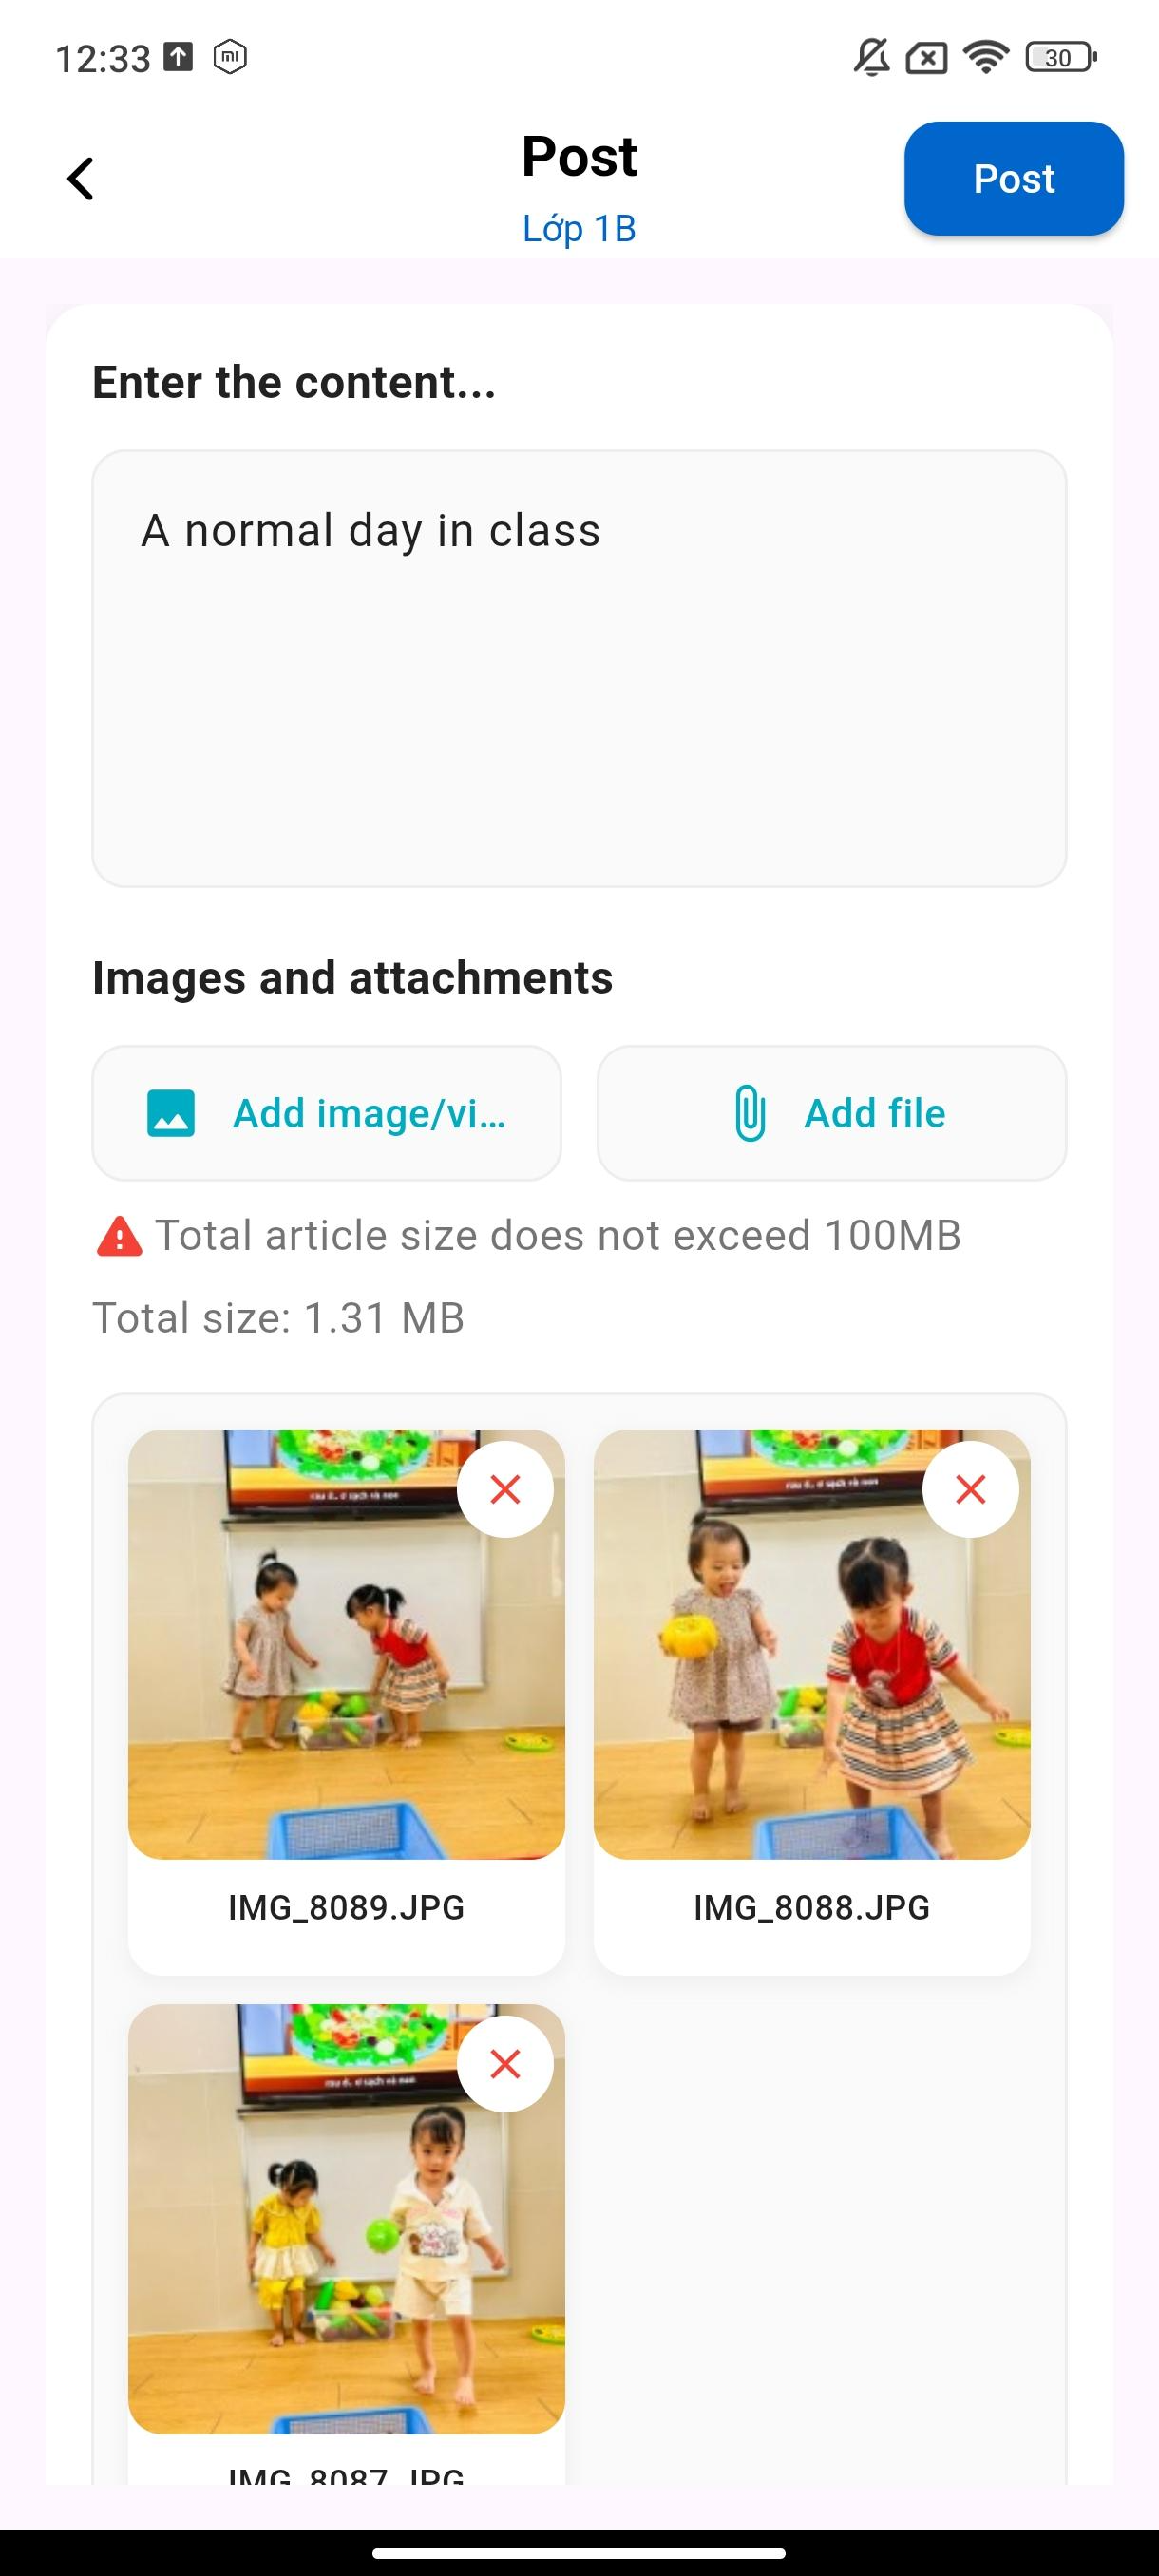
\includegraphics[width=0.6\textwidth]{images/create_post_teacher.png}
        \caption{Create Post Teacher View}
        \label{subfig:create_post_teacher_view}
    \end{subfigure}
    \hfill
    \begin{subfigure}{0.45\textwidth}
        \centering
        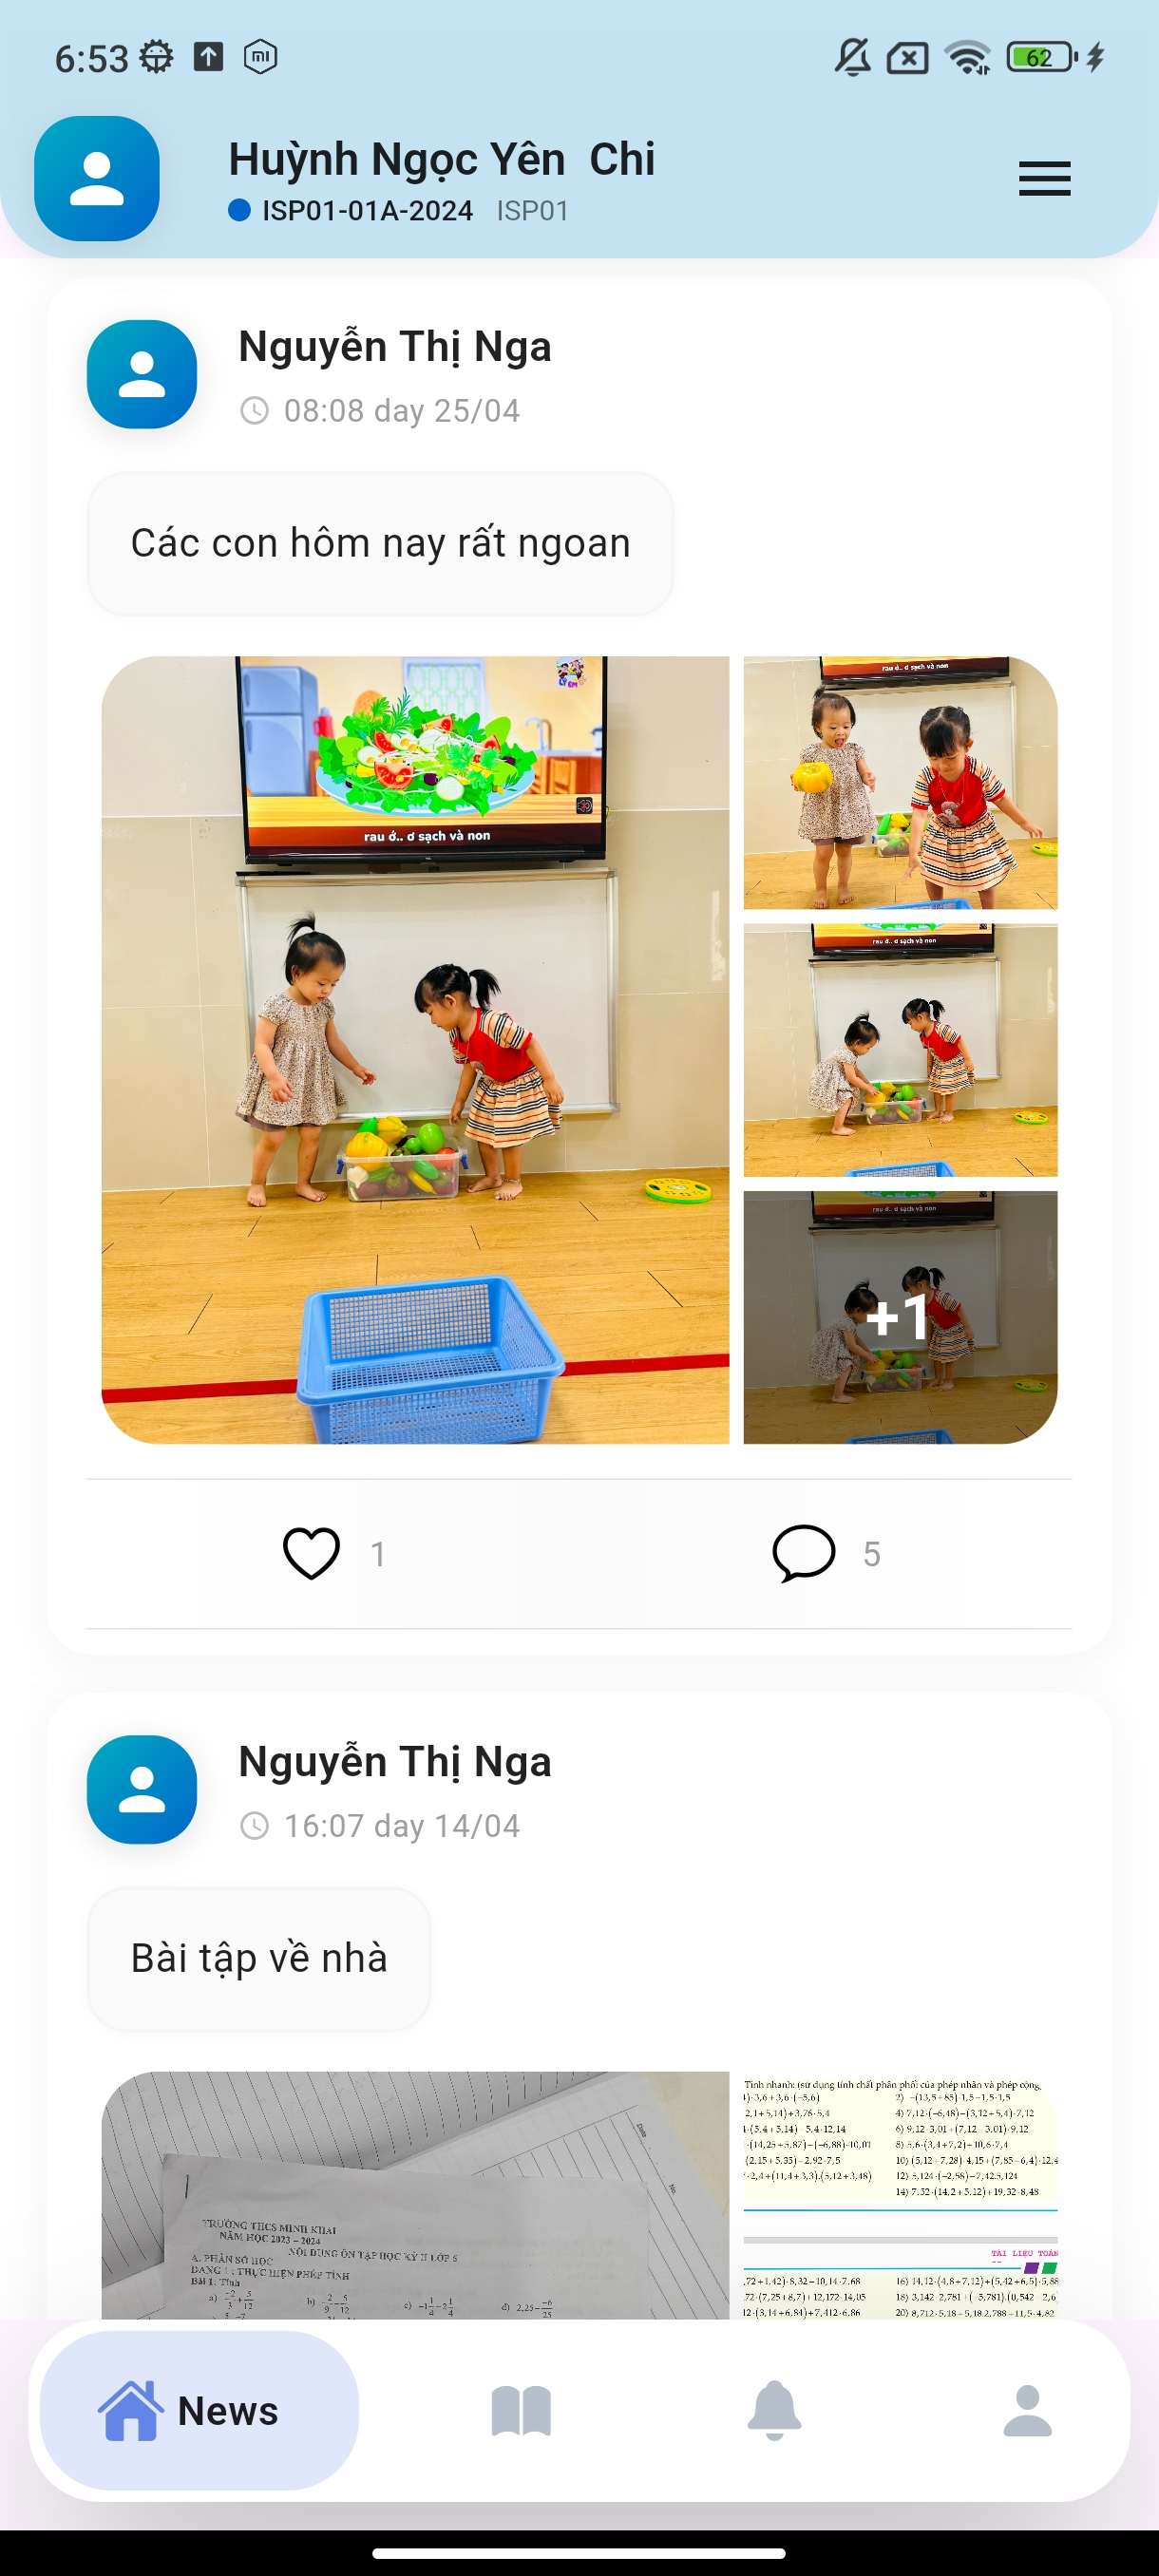
\includegraphics[width=0.6\textwidth]{images/appendix_news_student_mobile}
        \caption{Newsfeed Parent View}
        \label{subfig:newsfeed_parent_view}
    \end{subfigure}
    \caption{Newsfeed mobile app}
    \label{fig:newsfeed_mobile_app}
    \end{figure}
    %--------------
    \item \textbf{Student Attendance Management}
    \begin{figure}[H]
    \centering
    \begin{subfigure}{0.45\textwidth}
        \centering
        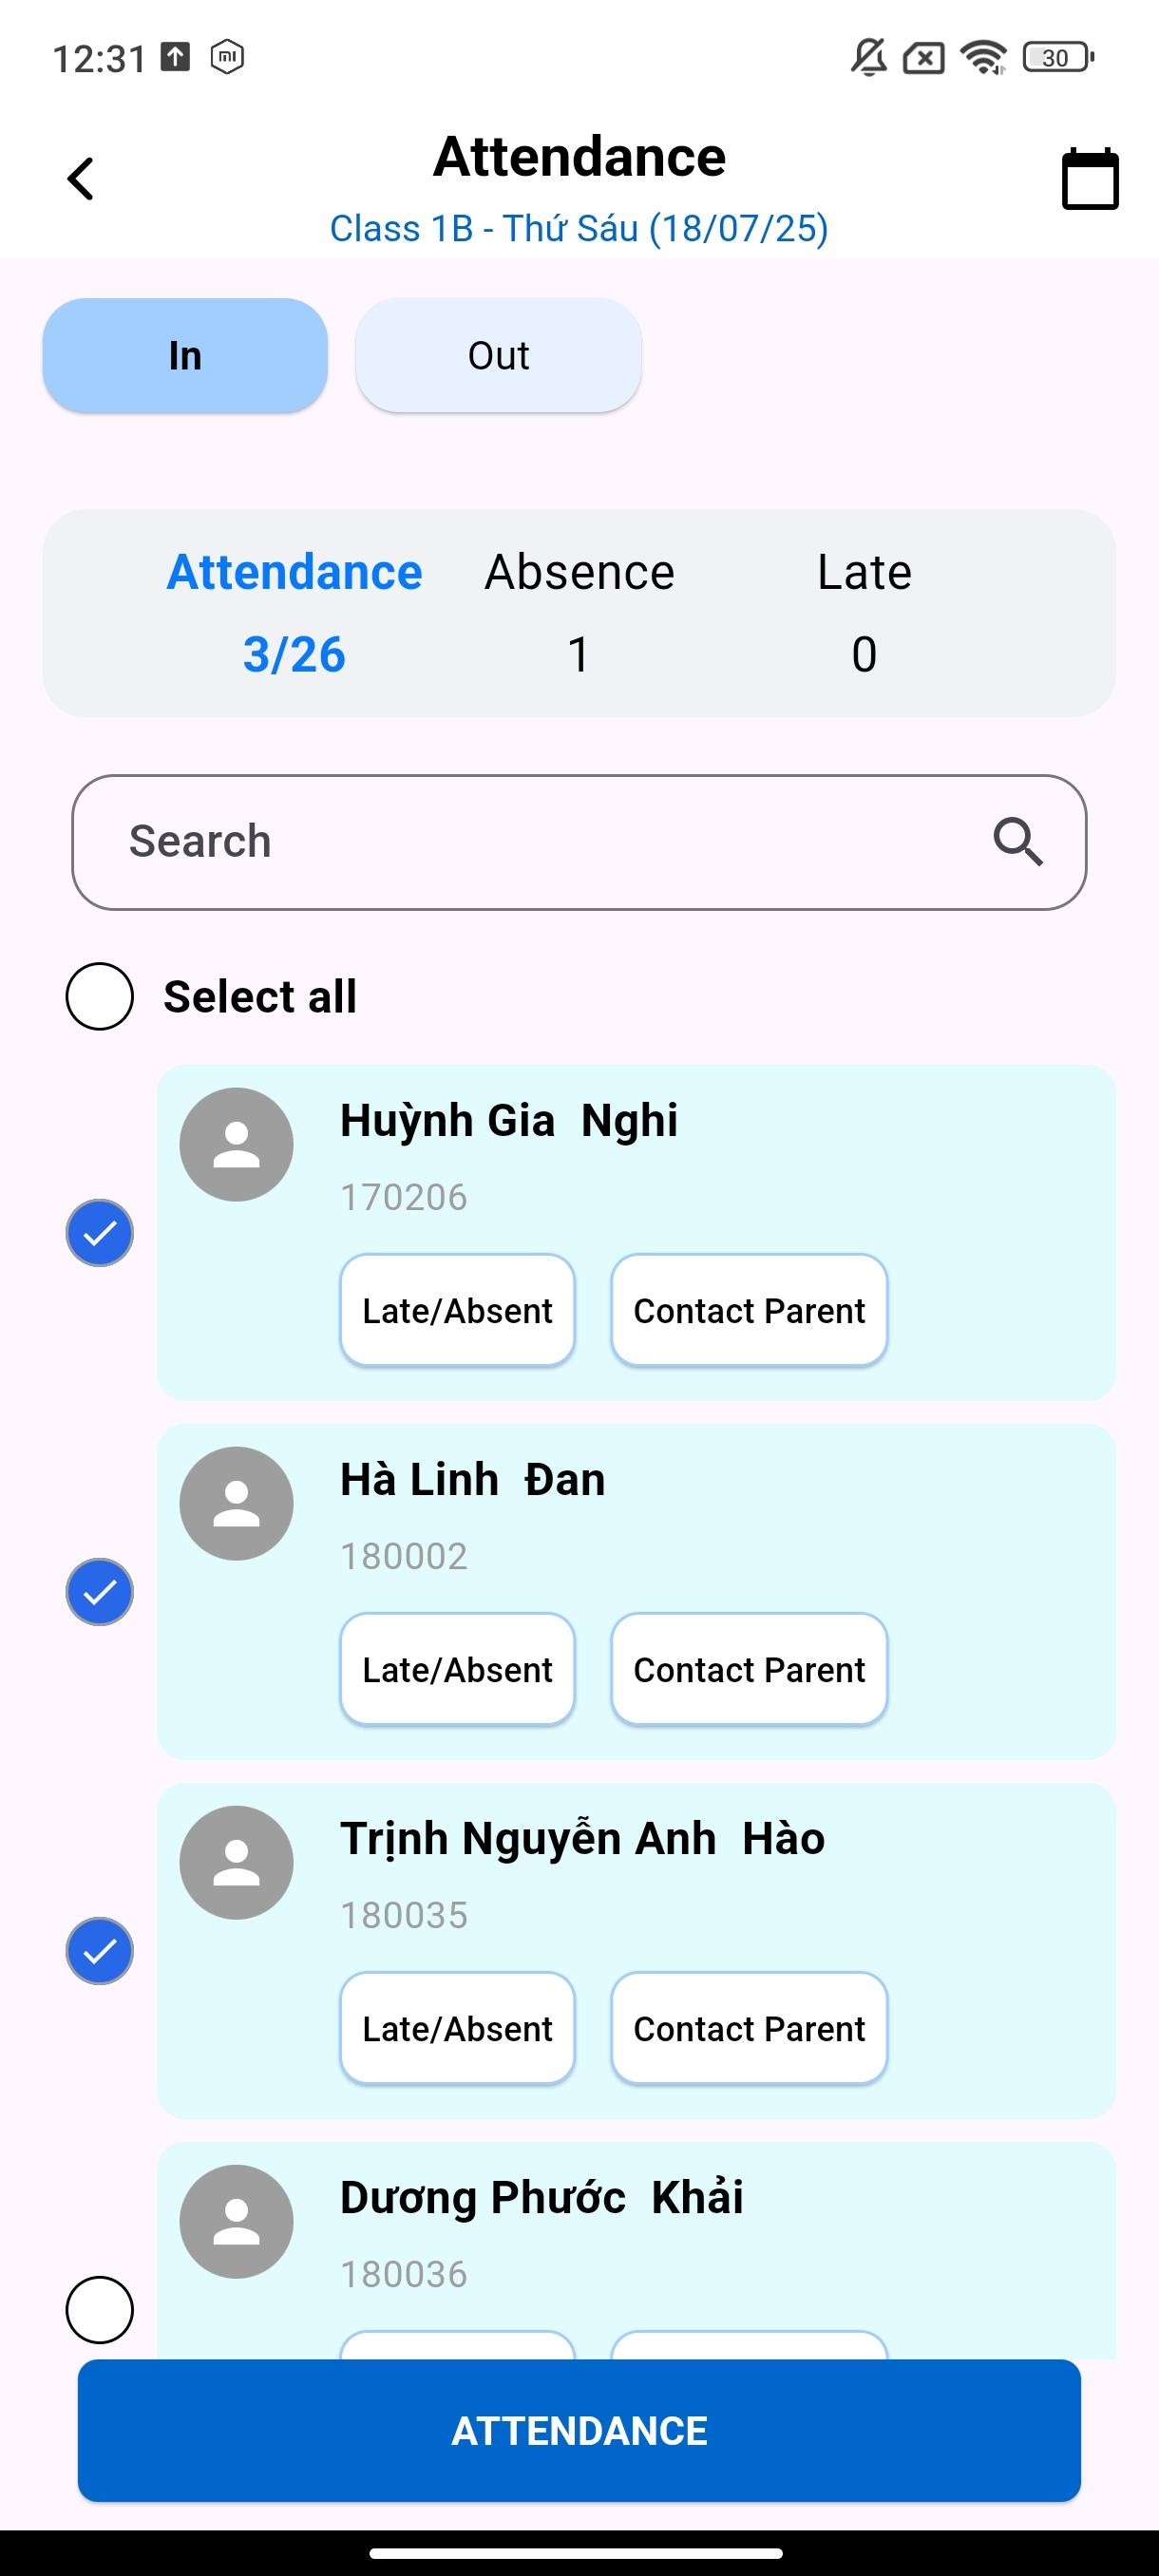
\includegraphics[width=0.6\textwidth]{images/attendance_teacher_view.png}
        \caption{Attendance - Teacher View}
        \label{subfig:attendance_teacher_view}
    \end{subfigure}
    \hfill
    \begin{subfigure}{0.45\textwidth}
        \centering
        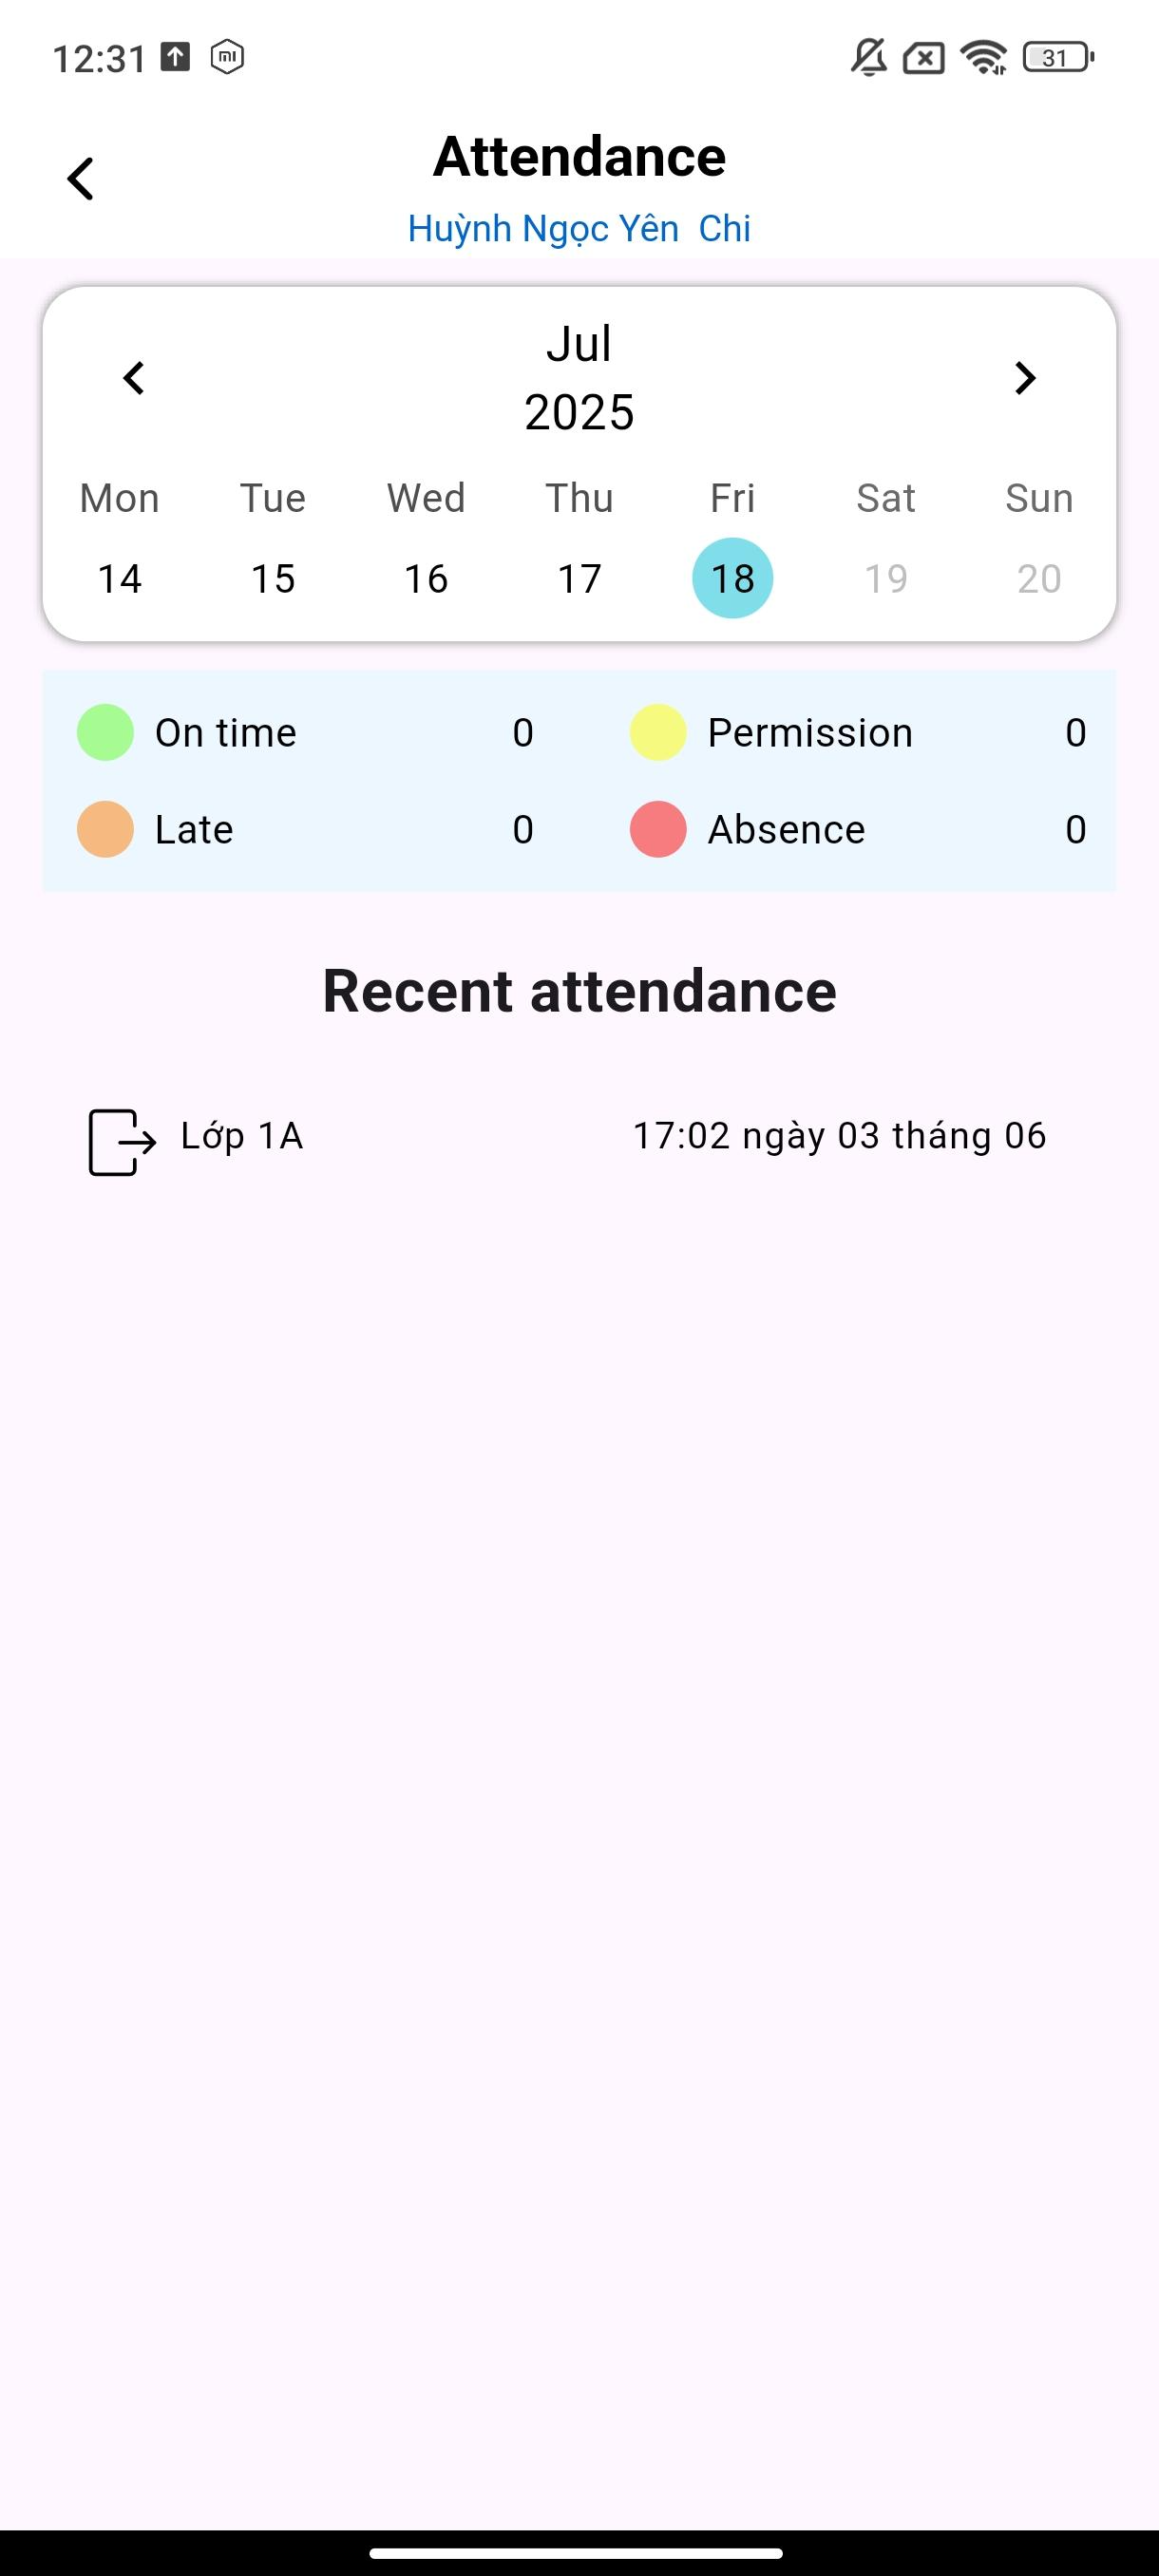
\includegraphics[width=0.6\textwidth]{images/attendance_parent_view.png}
        \caption{Attendance - Parent View}
        \label{subfig:attendance_parent_view}
    \end{subfigure}
    \caption{Attendance mobile app}
    \label{fig:attendance_mobile_app}
    \end{figure}
    \begin{figure}[H]
    \centering
    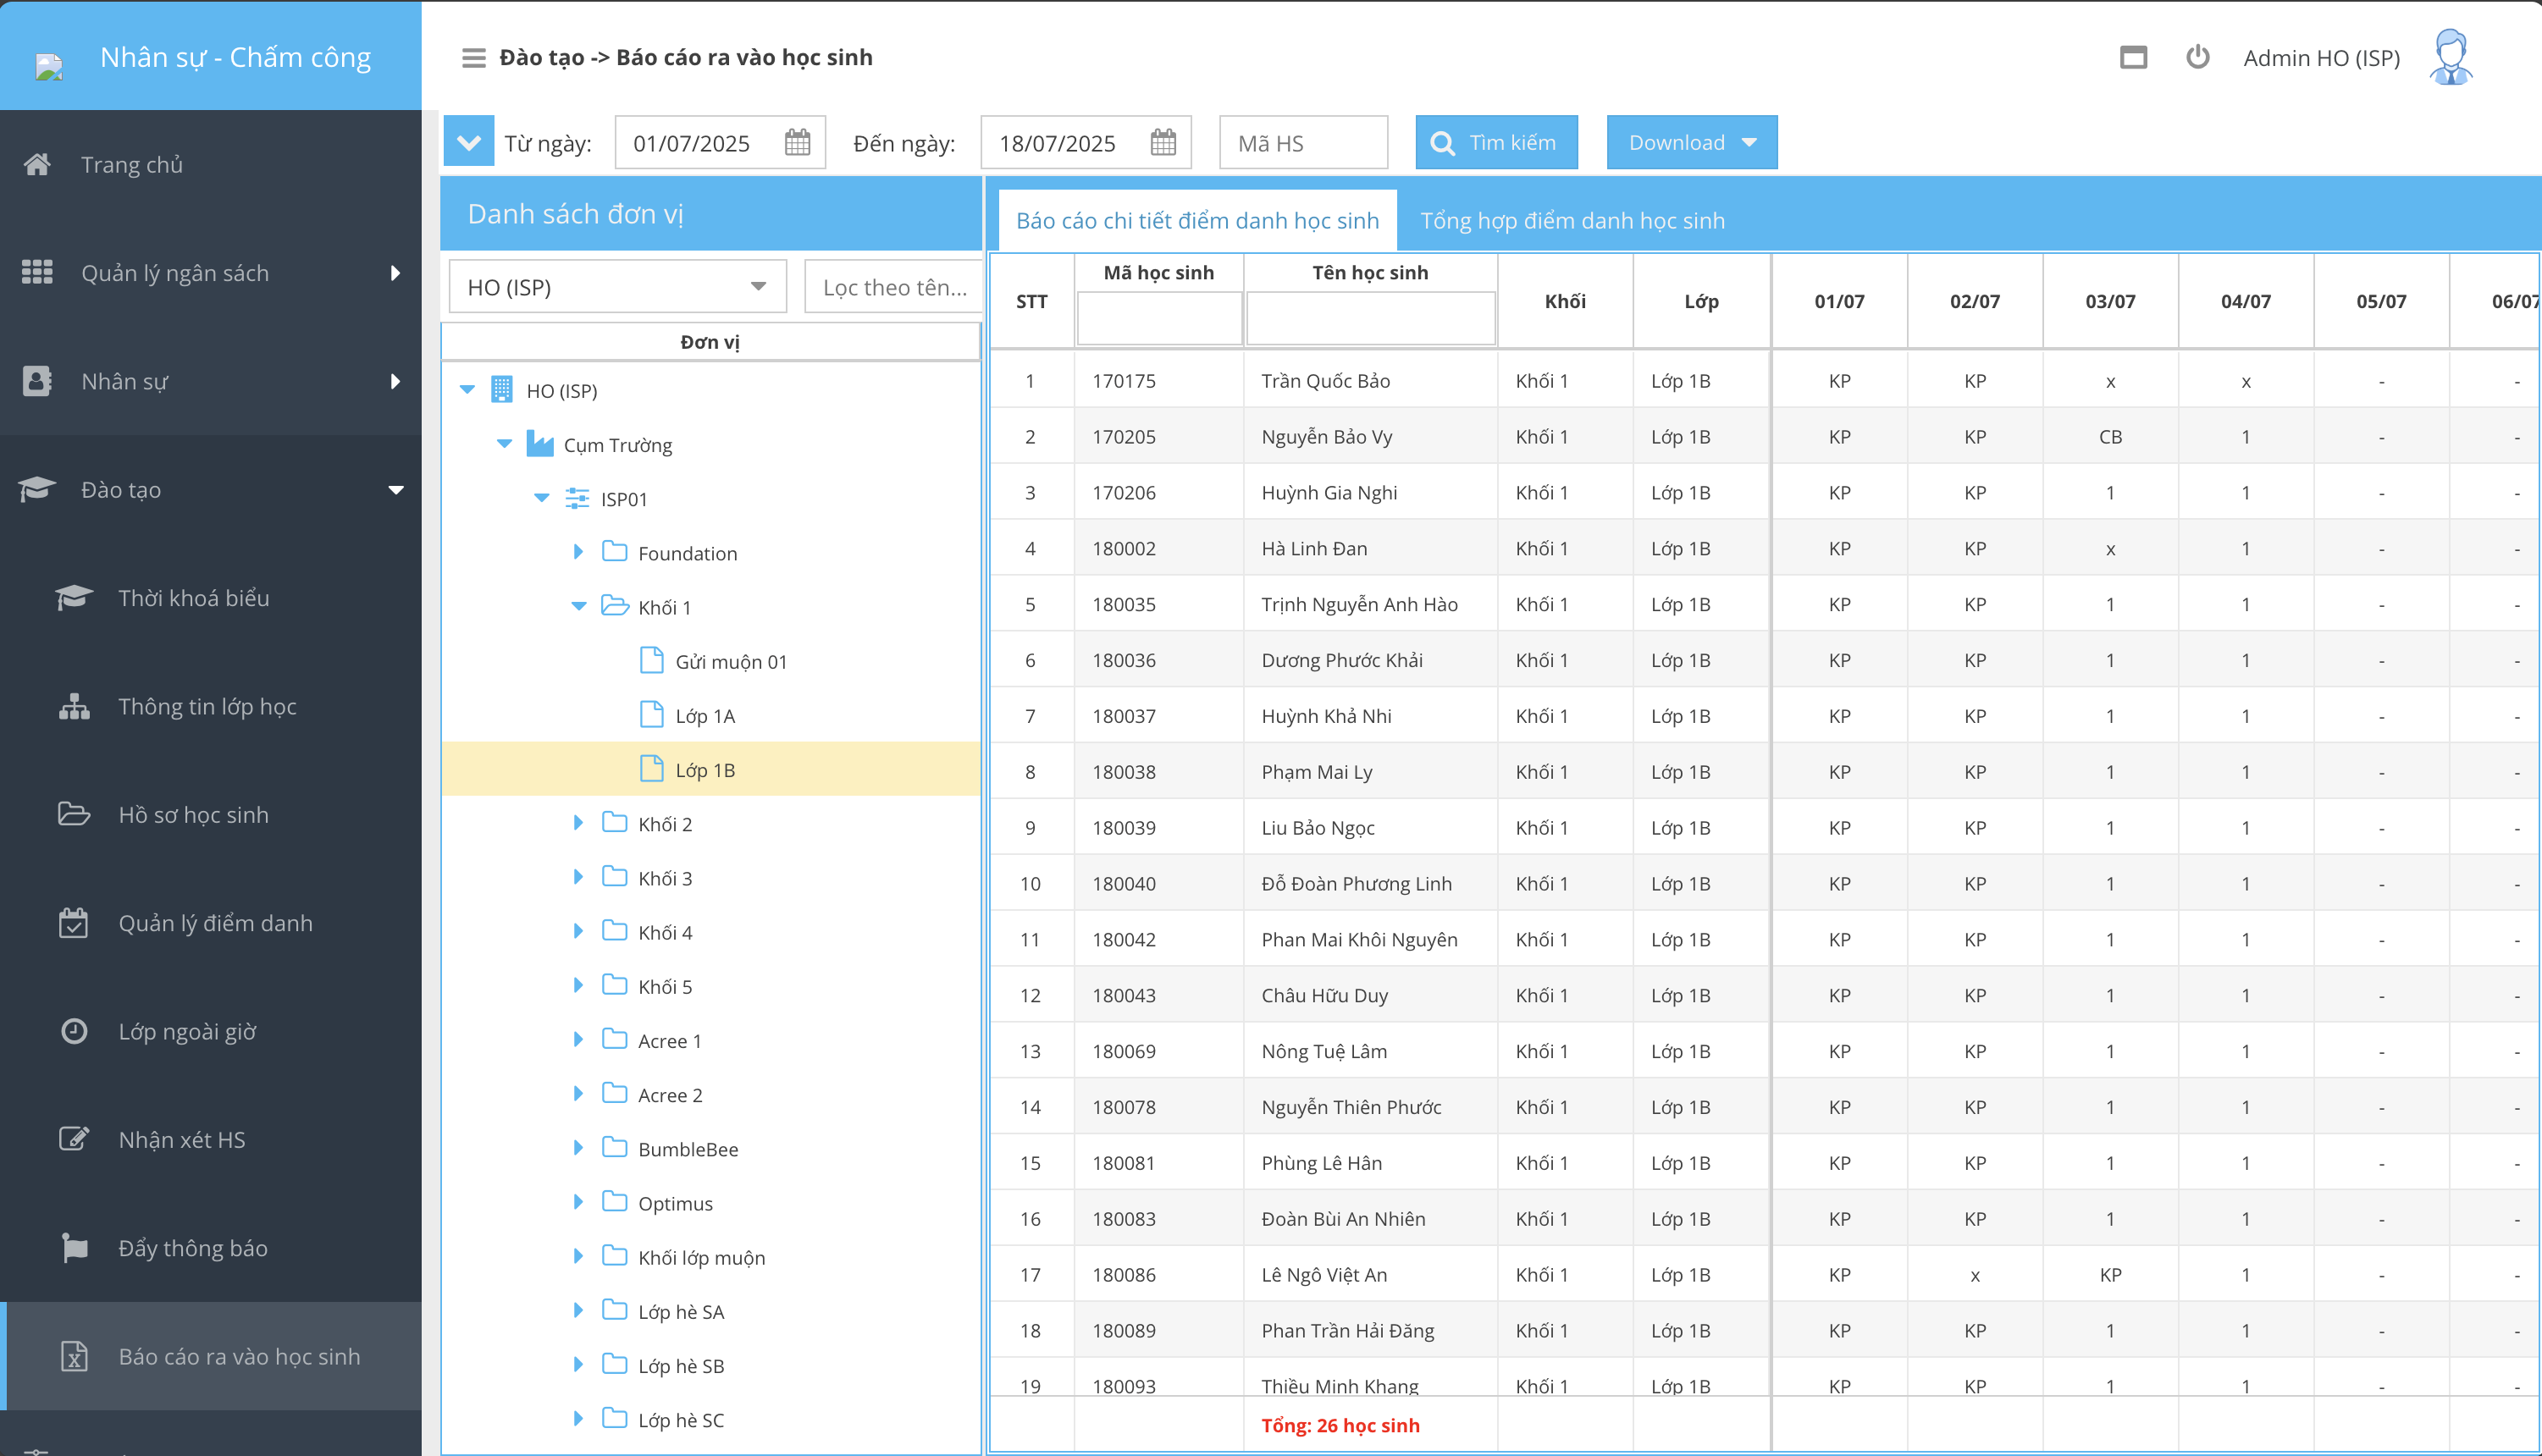
\includegraphics[width=1\textwidth]{images/student_attendance_report.png}
    \vspace{-1em}
    \caption{Student attendance report web app.}
    \label{fig:attendance_report_web}
    \end{figure}
    %--------------
    \item \textbf{Student Assessments Management}
    \begin{figure}[H]
    \centering
    \begin{subfigure}{0.45\textwidth}
        \centering
        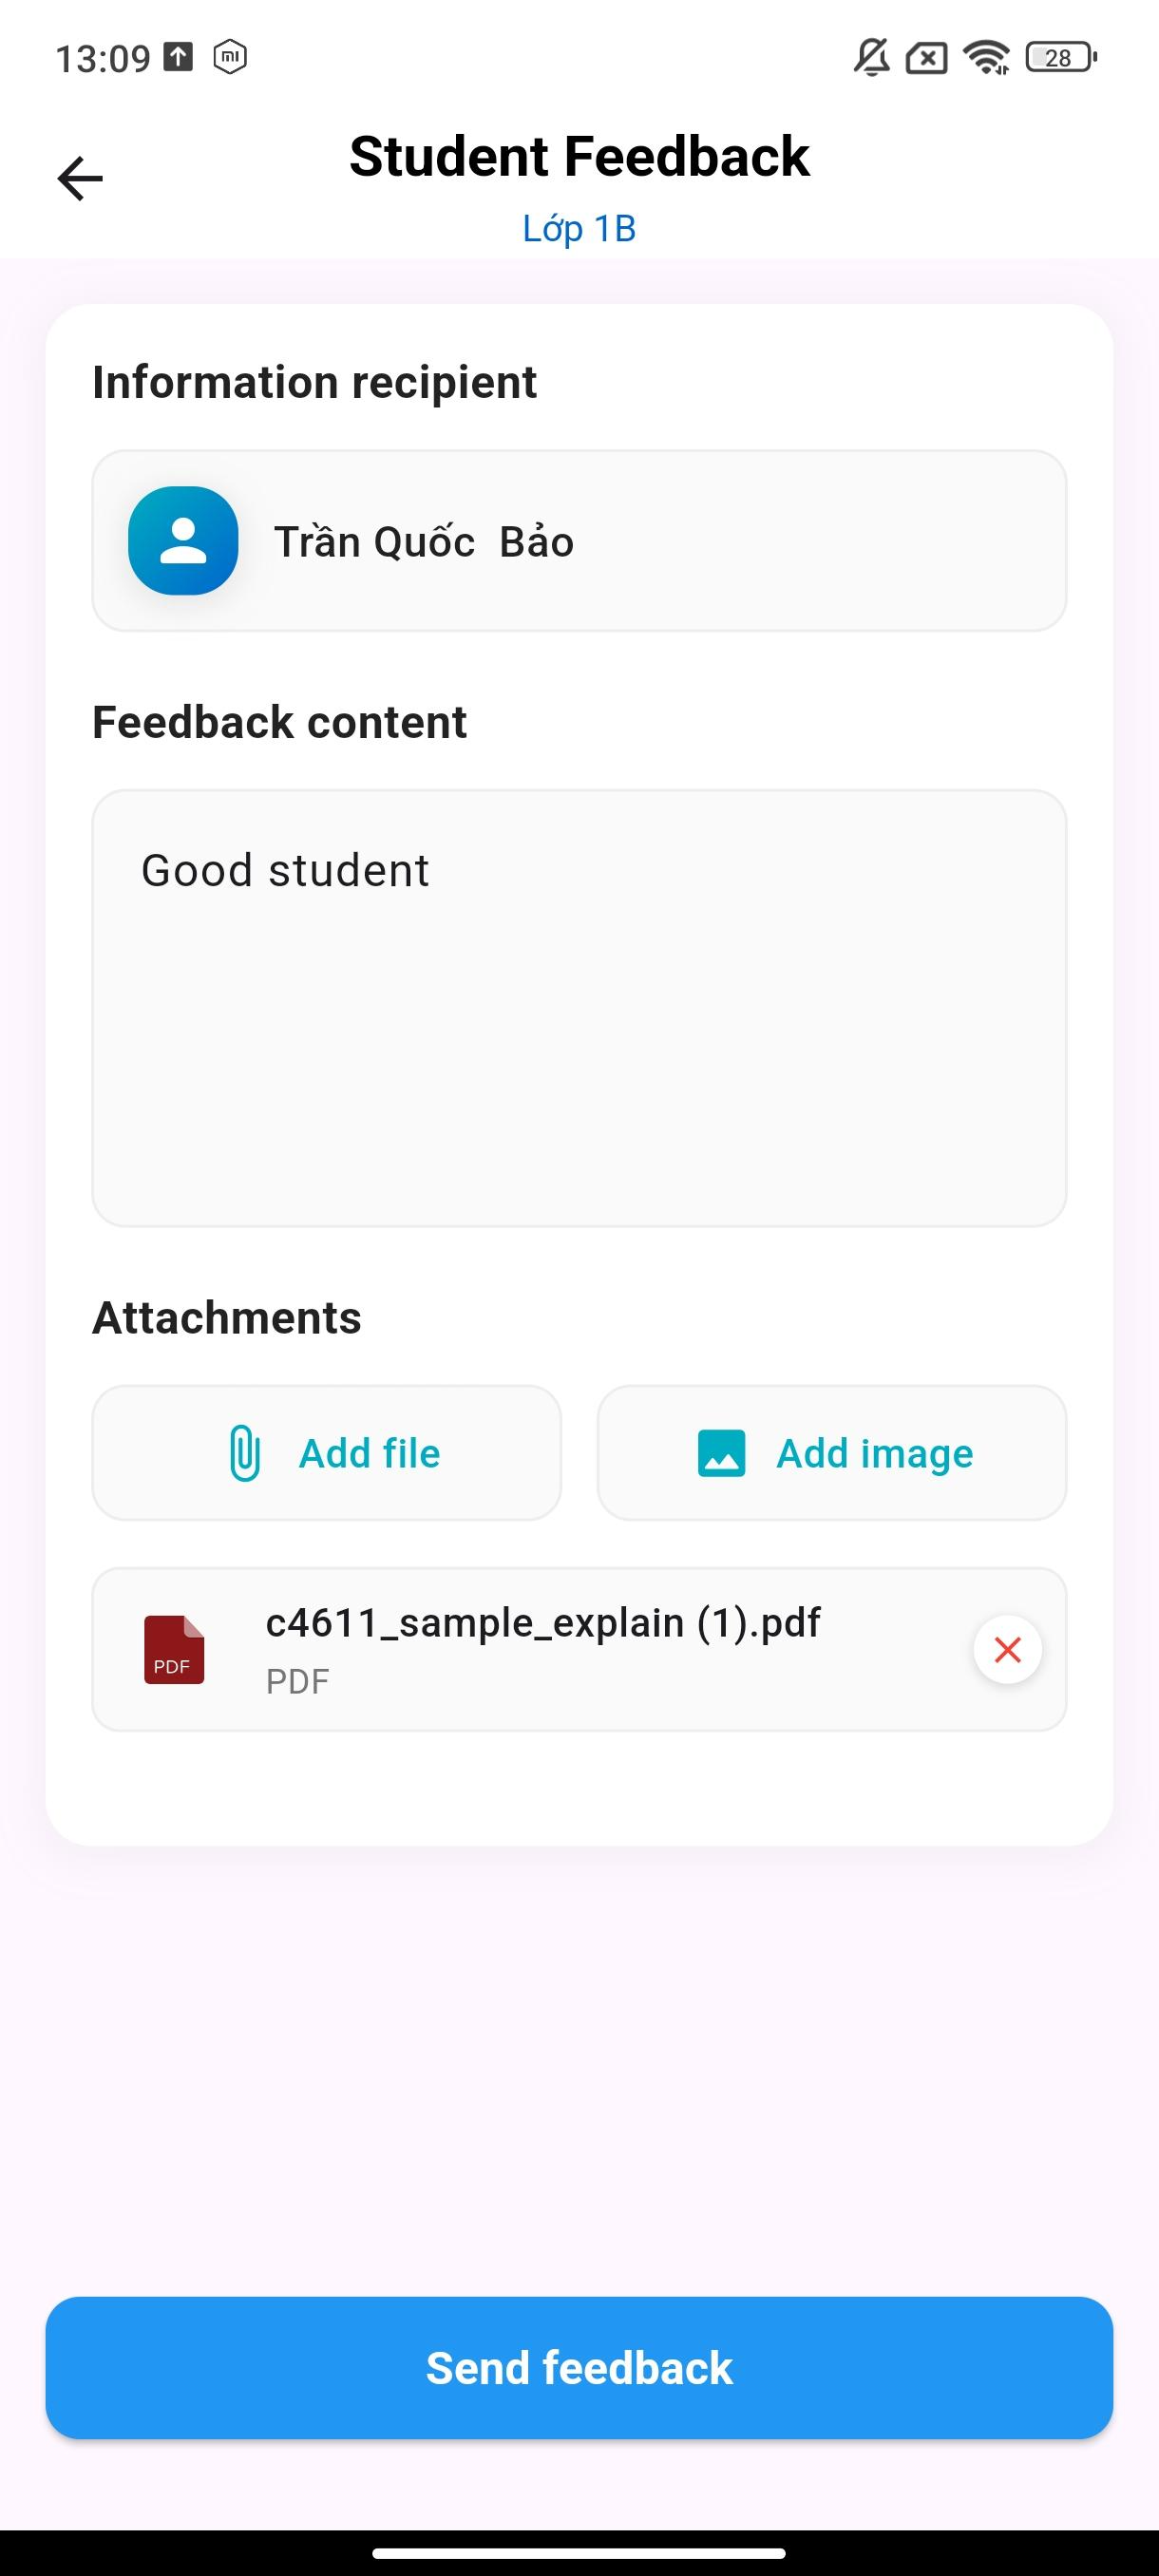
\includegraphics[width=0.6\textwidth]{images/assess_teacher_view.png}
        \caption{Assess Student - Teacher View}
        \label{subfig:assess_student_teacher_view}
    \end{subfigure}
    \hfill
    \begin{subfigure}{0.45\textwidth}
        \centering
        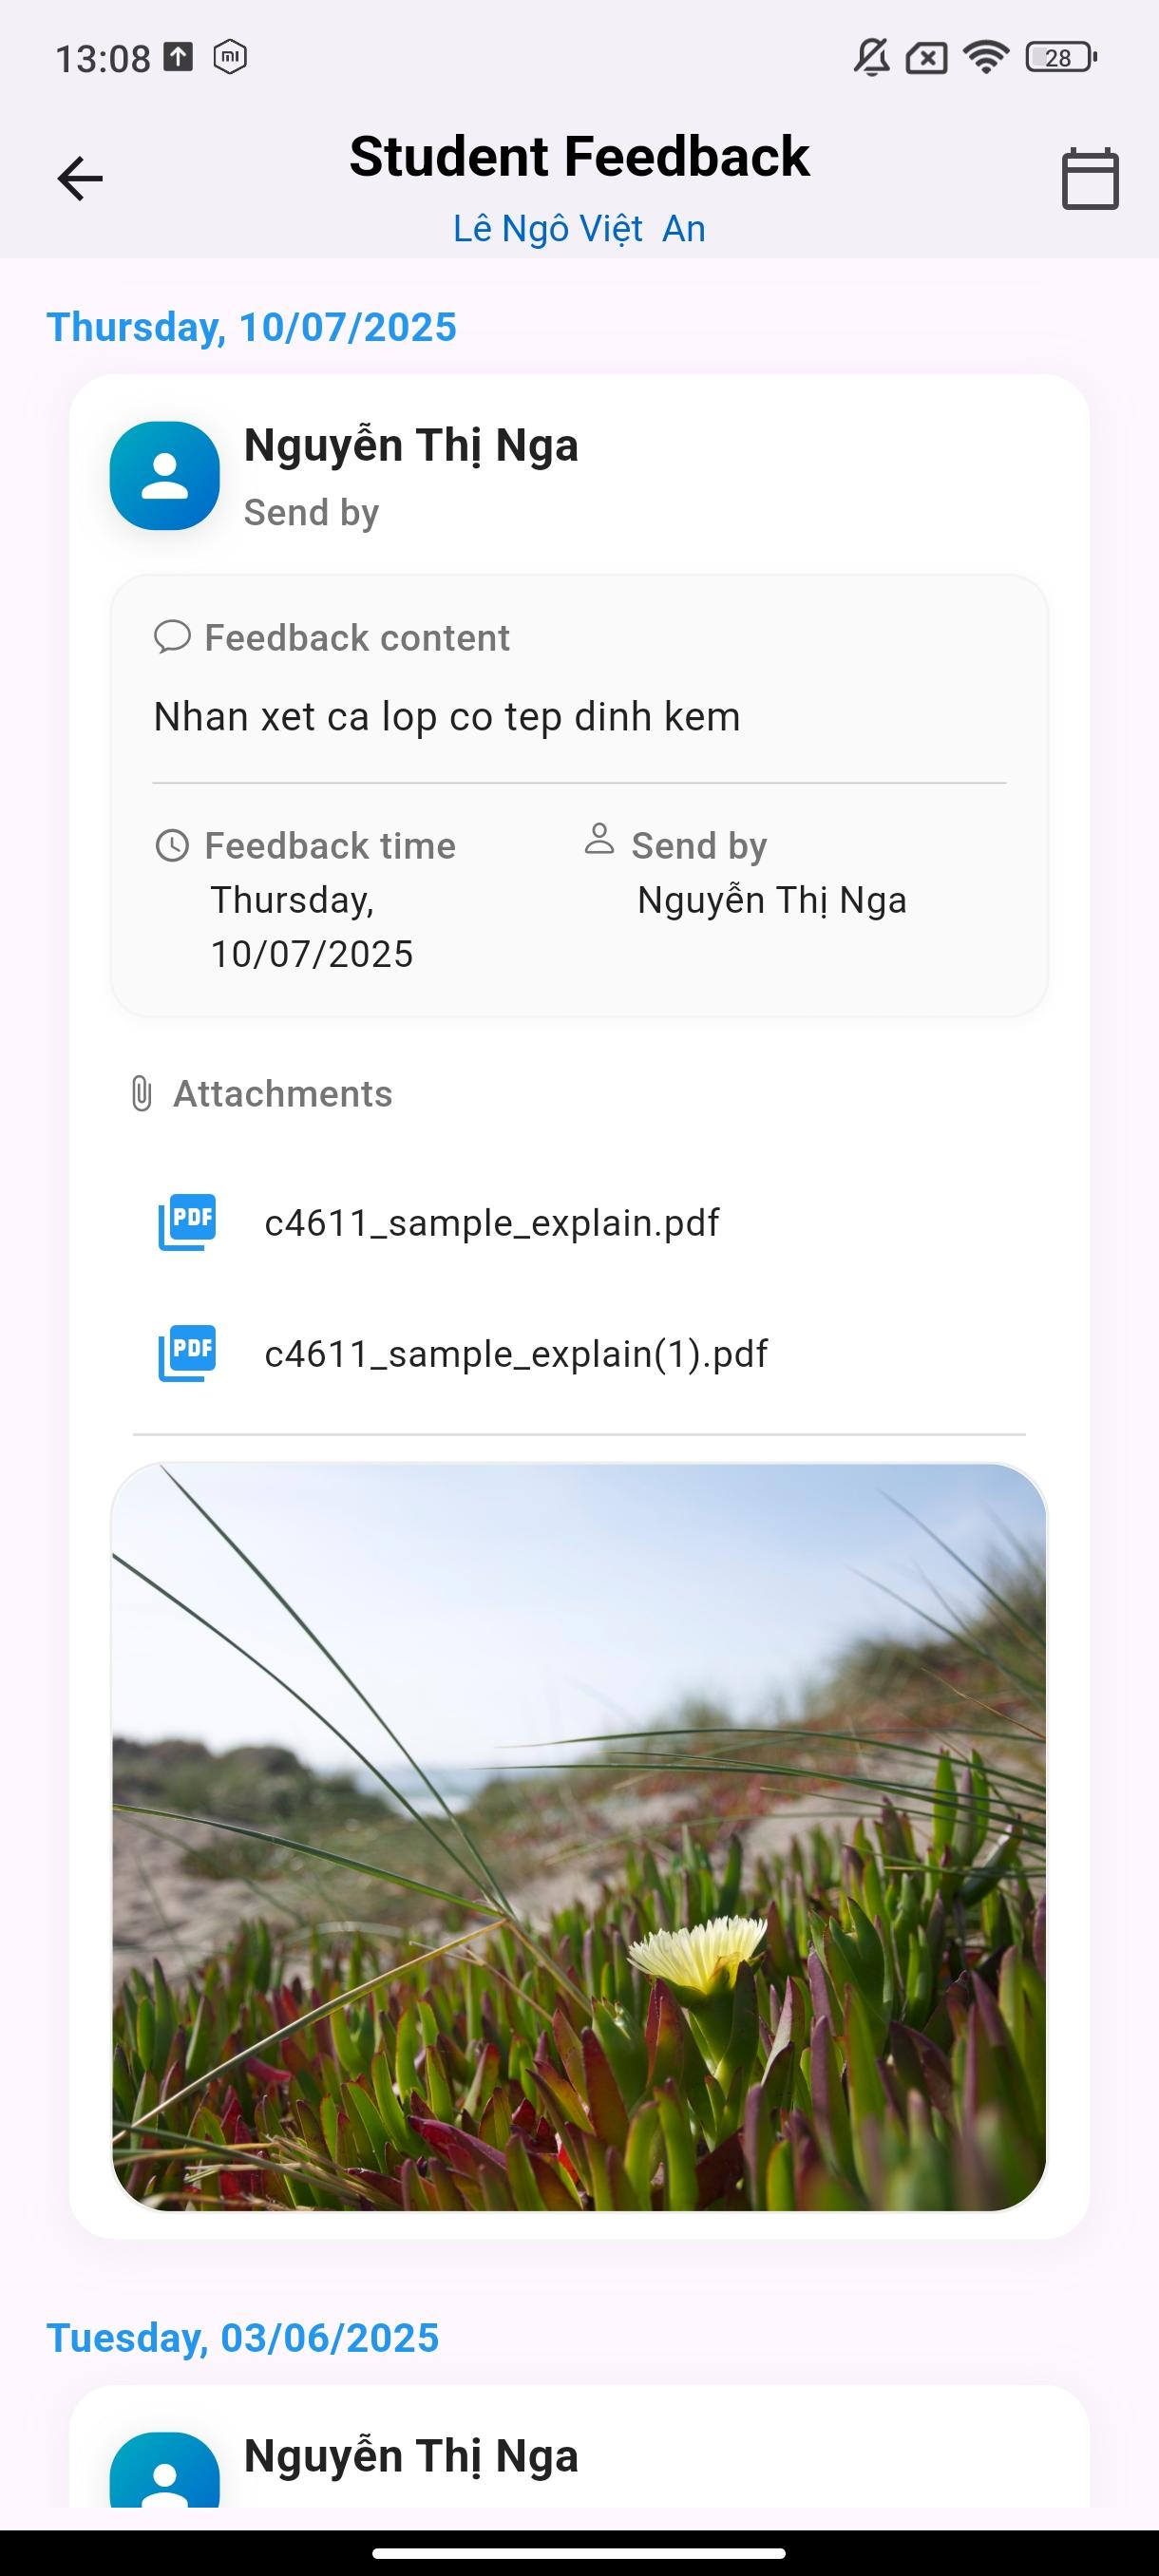
\includegraphics[width=0.6\textwidth]{images/assess_student_view.png}
        \caption{Assess Student - Parent View}
        \label{subfig:assess_student_parent_view}
    \end{subfigure}
    \caption{Assess Student mobile app}
    \label{fig:assess_student_mobile_app}
    \end{figure}
    %---------------------
    \newpage
    \item \textbf{Medicine Reminder Management}
    \begin{figure}[H]
    \centering
    \begin{subfigure}{0.45\textwidth}
        \centering
        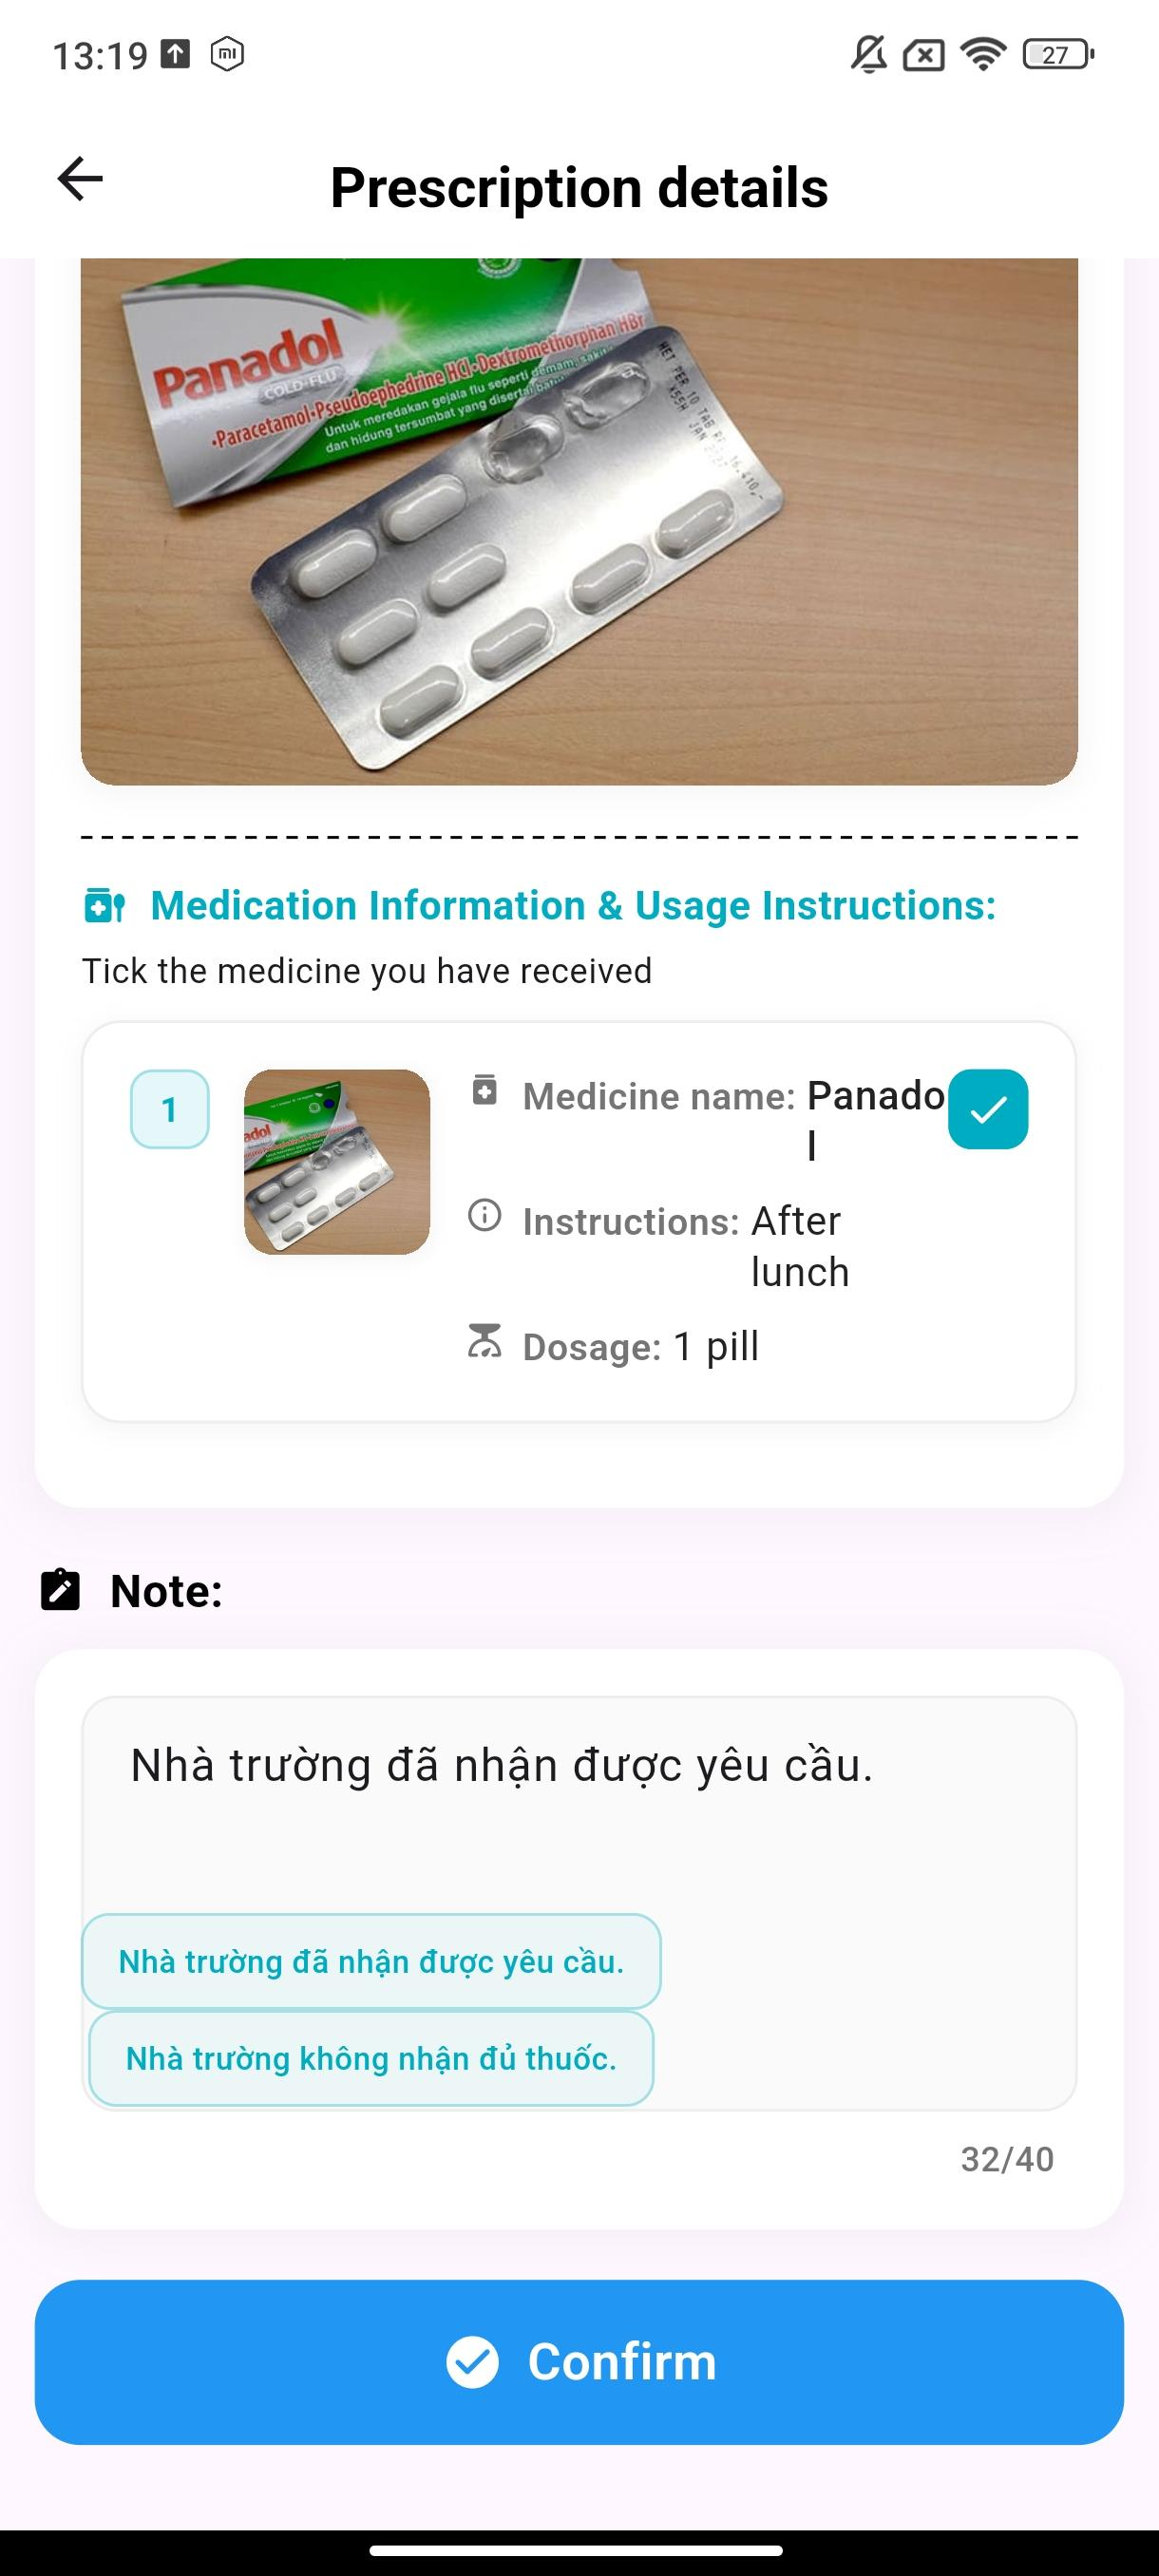
\includegraphics[width=0.6\textwidth]{images/medicine_reminder_confirmation_teacher.png}
        \caption{Medicine Reminder - Teacher Confimation View}
        \label{subfig:medicine_reminder_teacher_view}
    \end{subfigure}
    \hfill
    \begin{subfigure}{0.45\textwidth}
        \centering
        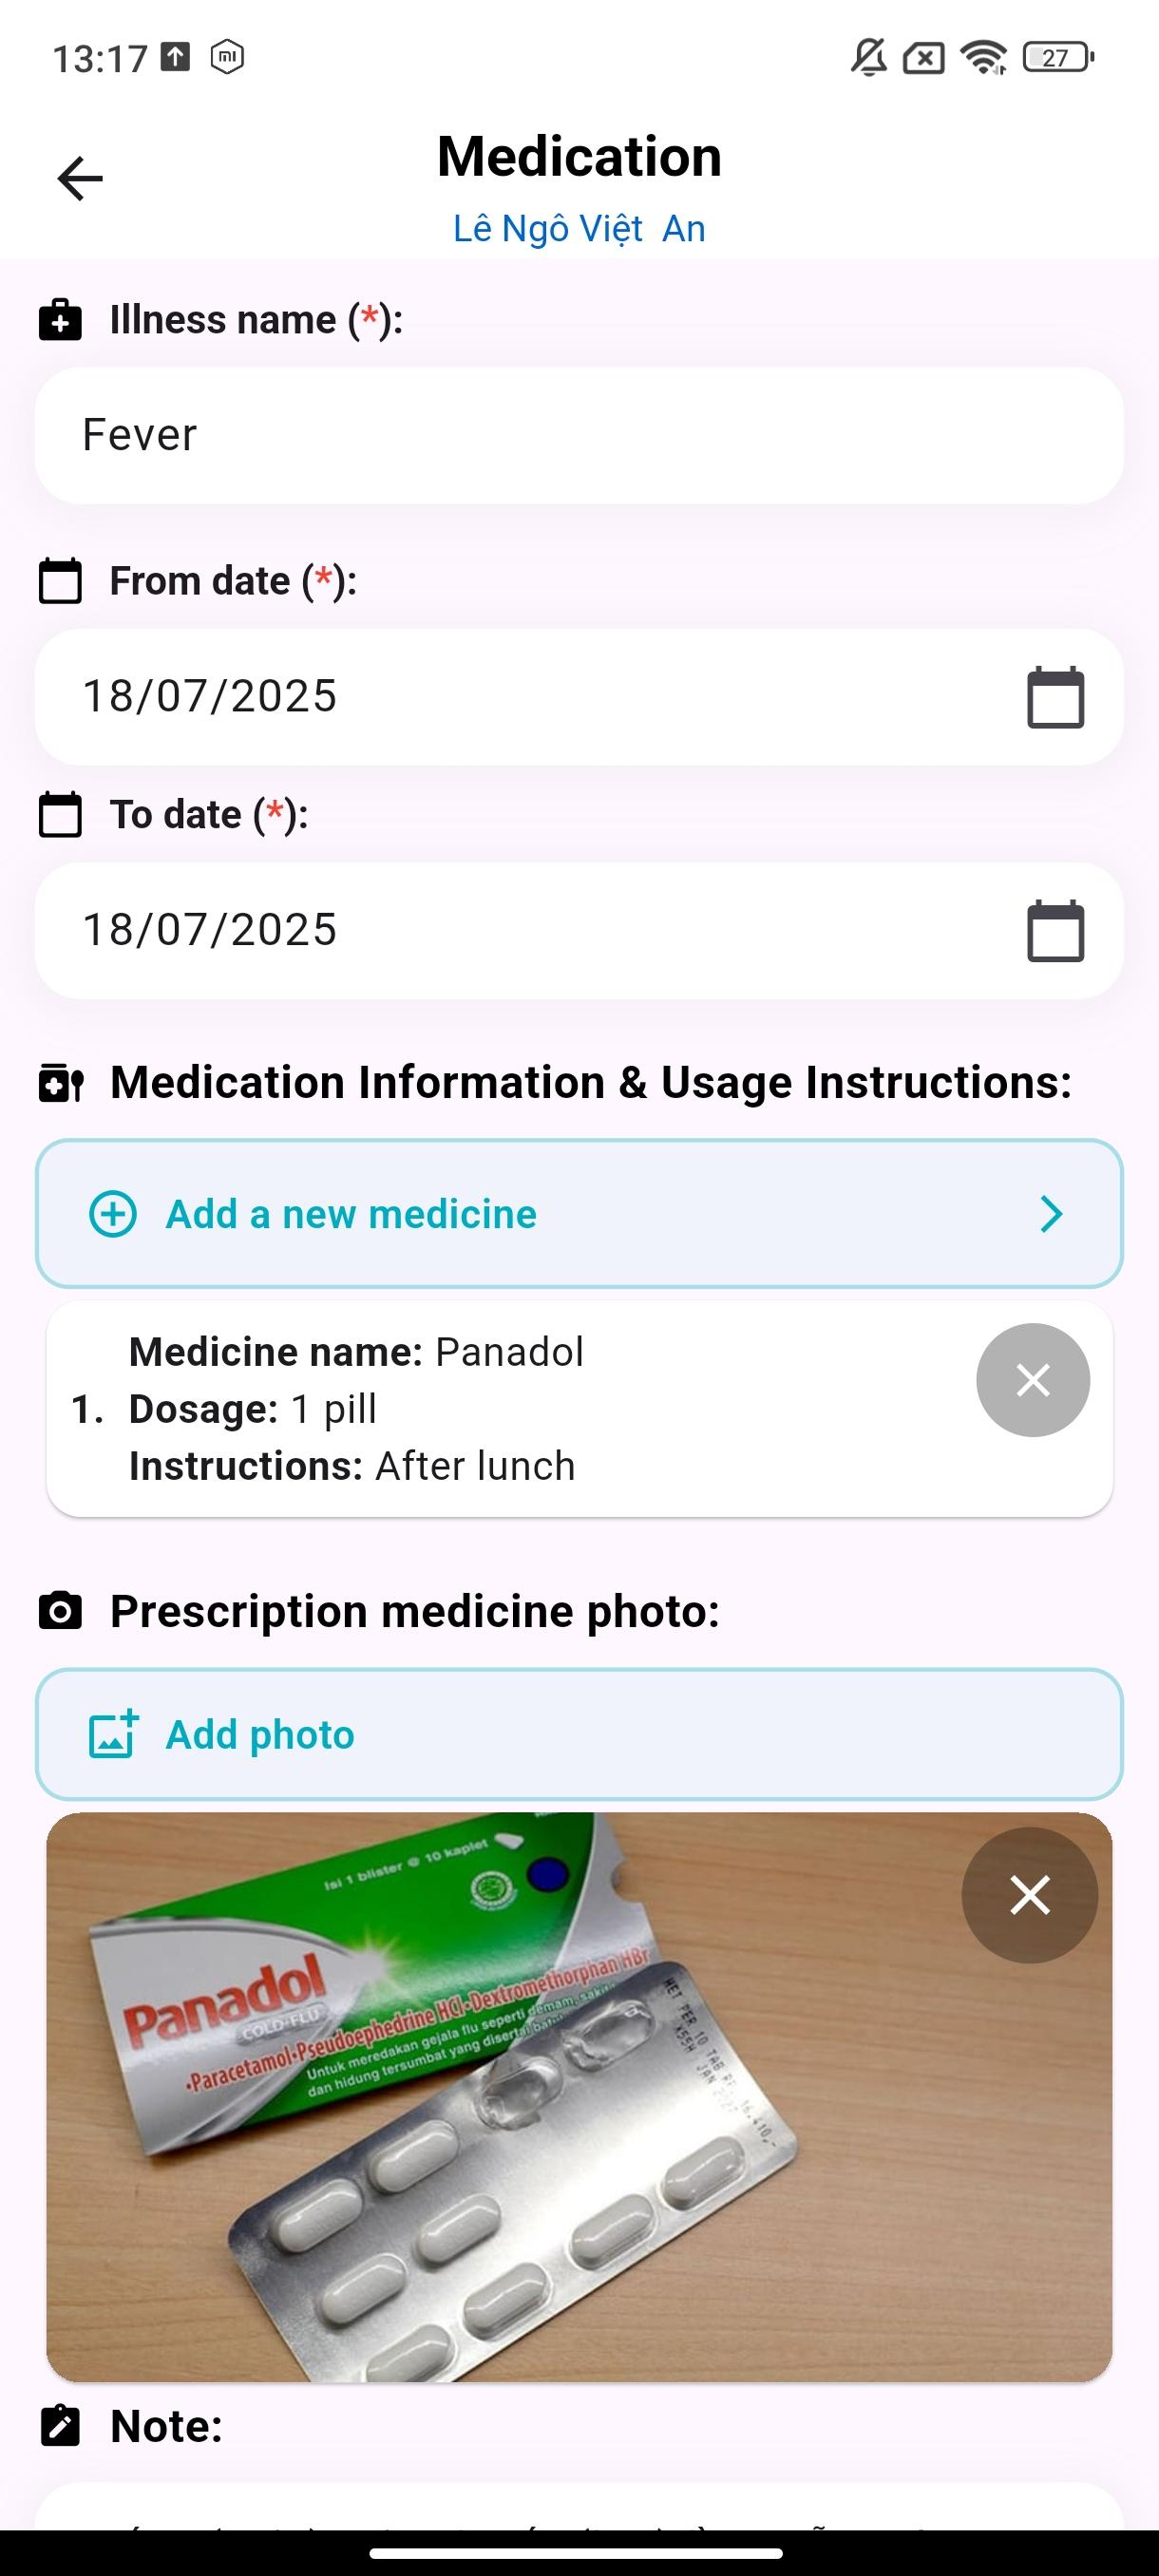
\includegraphics[width=0.6\textwidth]{images/medicine_reminder_parent_view.png}
        \caption{Medicine Reminder - Parent Create View}
        \label{subfig:medicine_reminder_parent_view}
    \end{subfigure}
    \caption{Medicine Reminder mobile app}
    \label{fig:medicine_reminder_mobile_app}
    \end{figure}
    %-----------------
    \item \textbf{Notification Management}
    \begin{figure}[H]
    \centering
    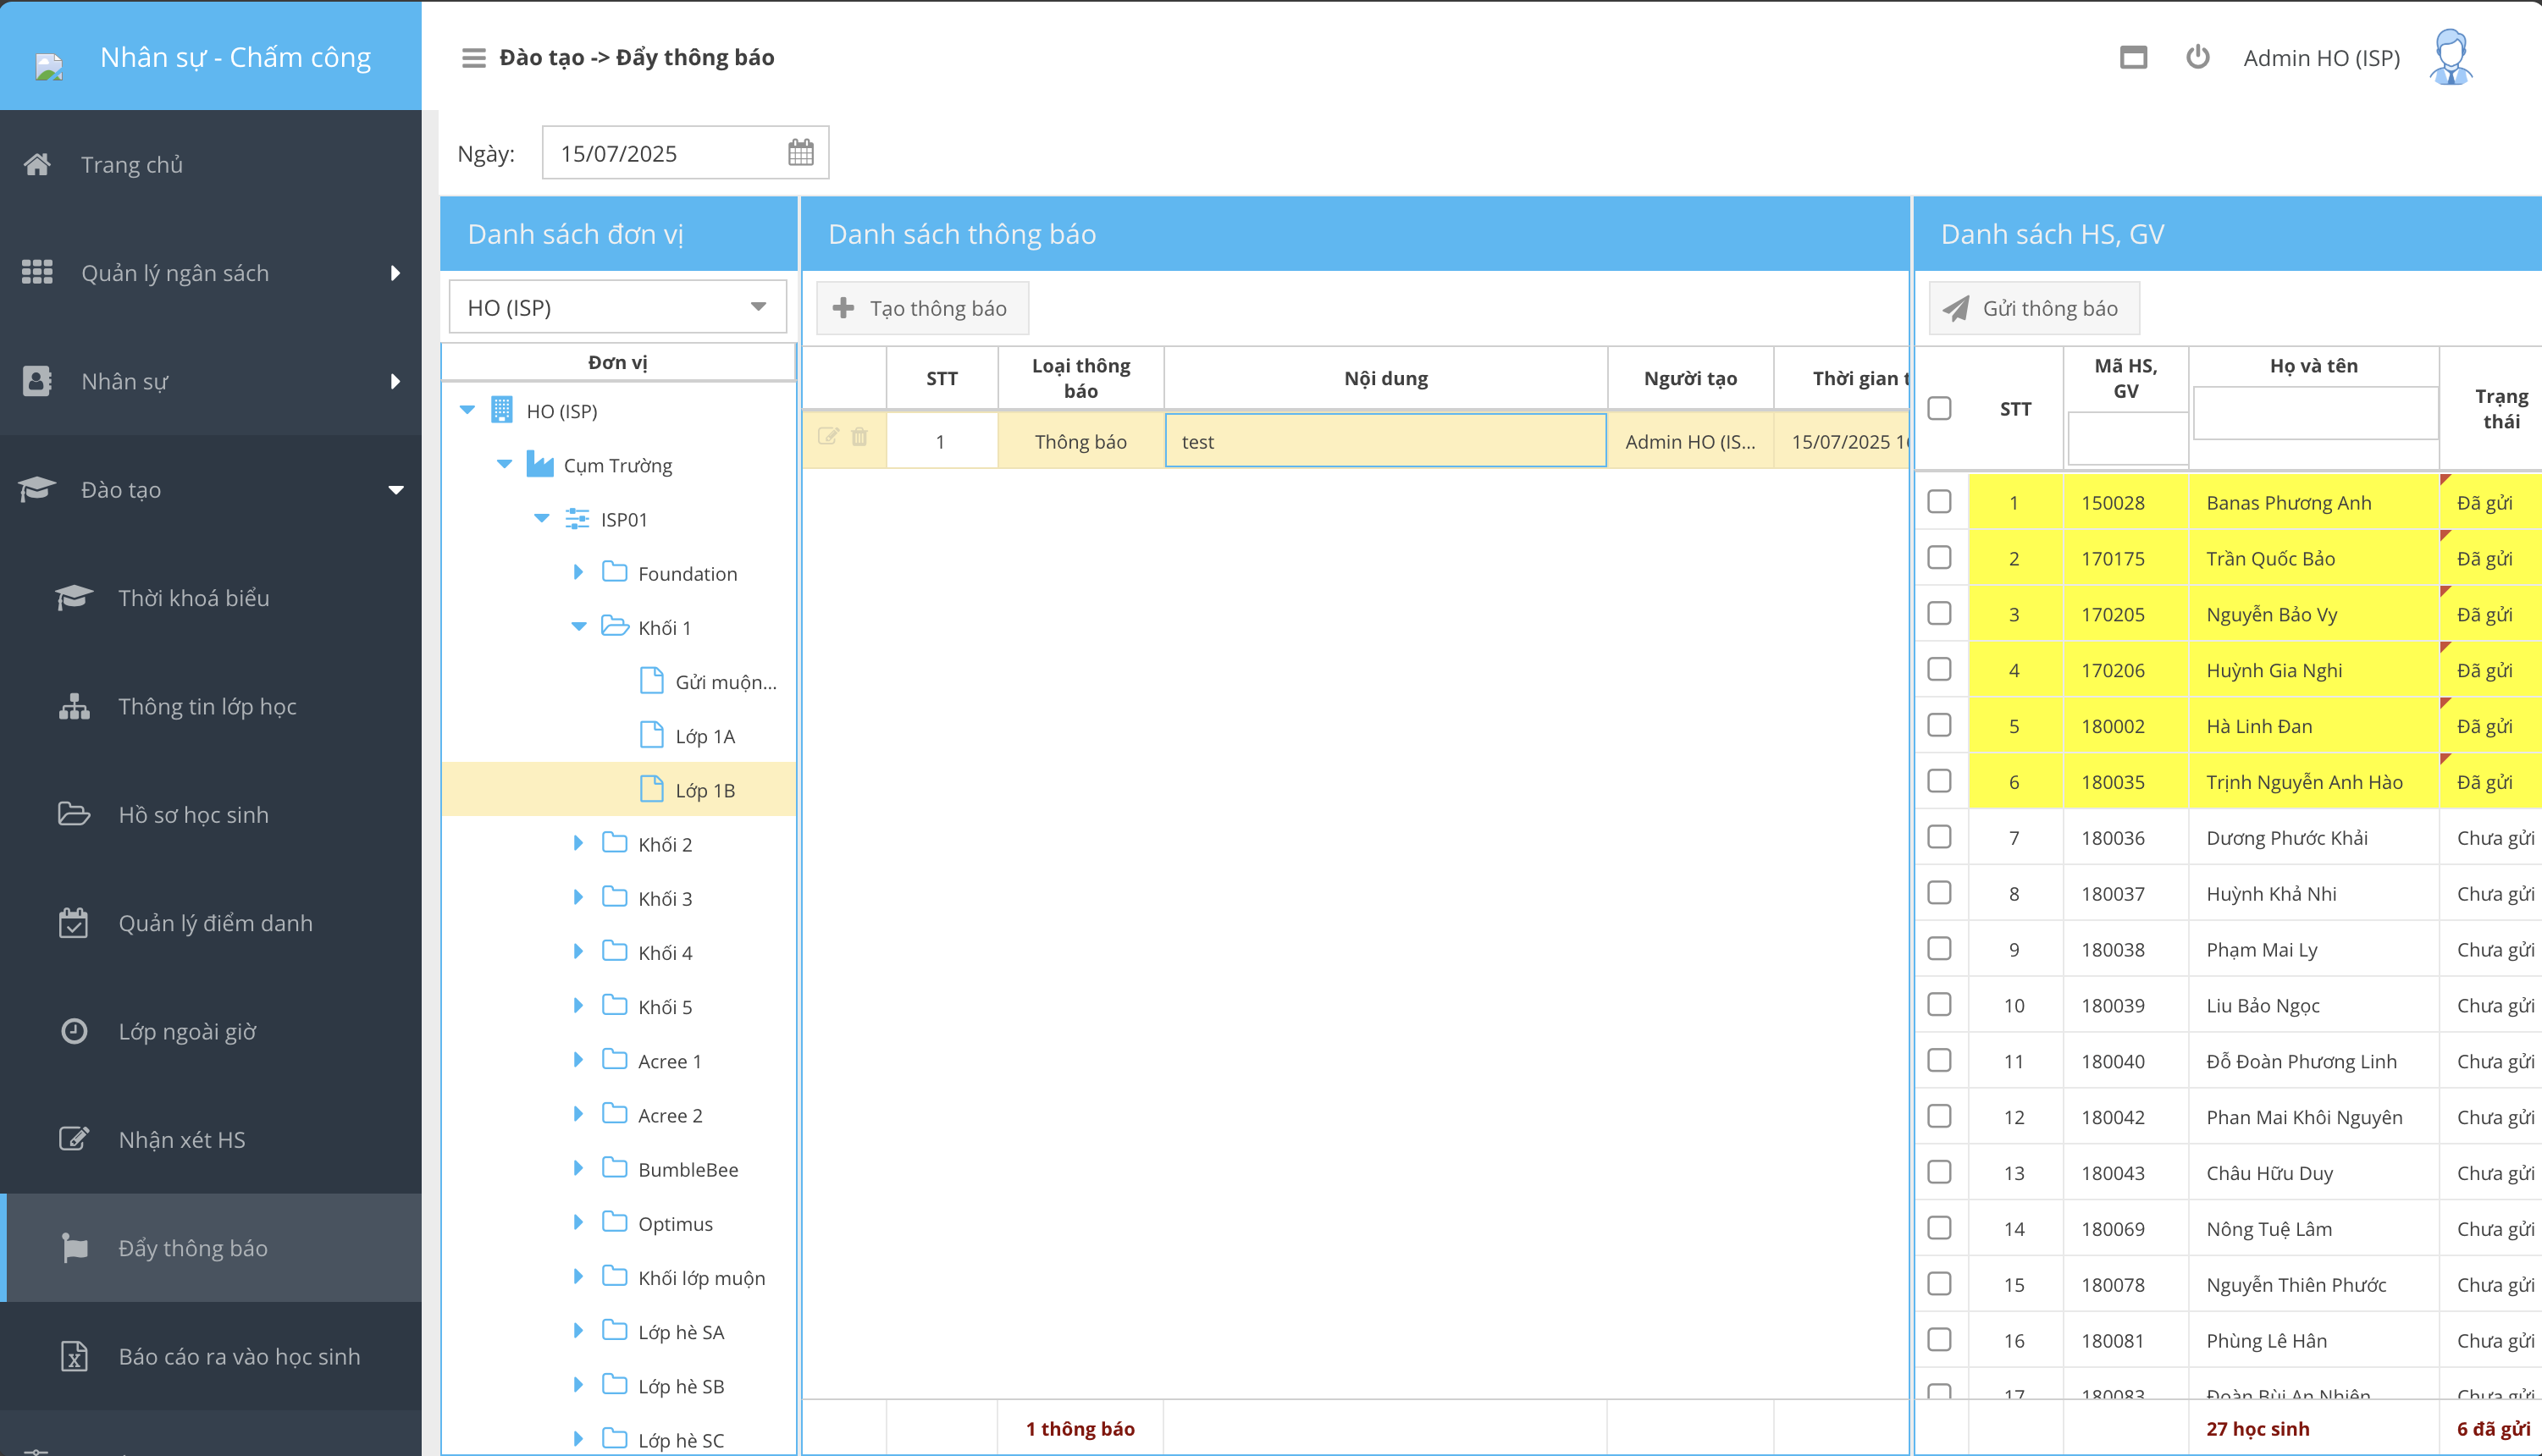
\includegraphics[width=1\textwidth]{images/notification_web.png}
    \vspace{-1em}
    \caption{Push notification web app.}
    \label{fig:push_notification_web}
    \end{figure}
    \begin{figure}[H]
    \centering
    \begin{subfigure}{0.45\textwidth}
        \centering
        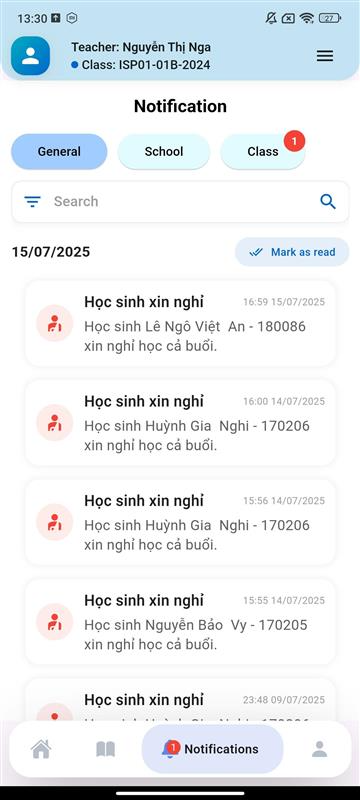
\includegraphics[width=0.6\textwidth]{images/notification_teacher_view.png}
        \caption{Notification - Teacher View}
        \label{subfig:notification_teacher_view}
    \end{subfigure}
    \hfill
    \begin{subfigure}{0.45\textwidth}
        \centering
        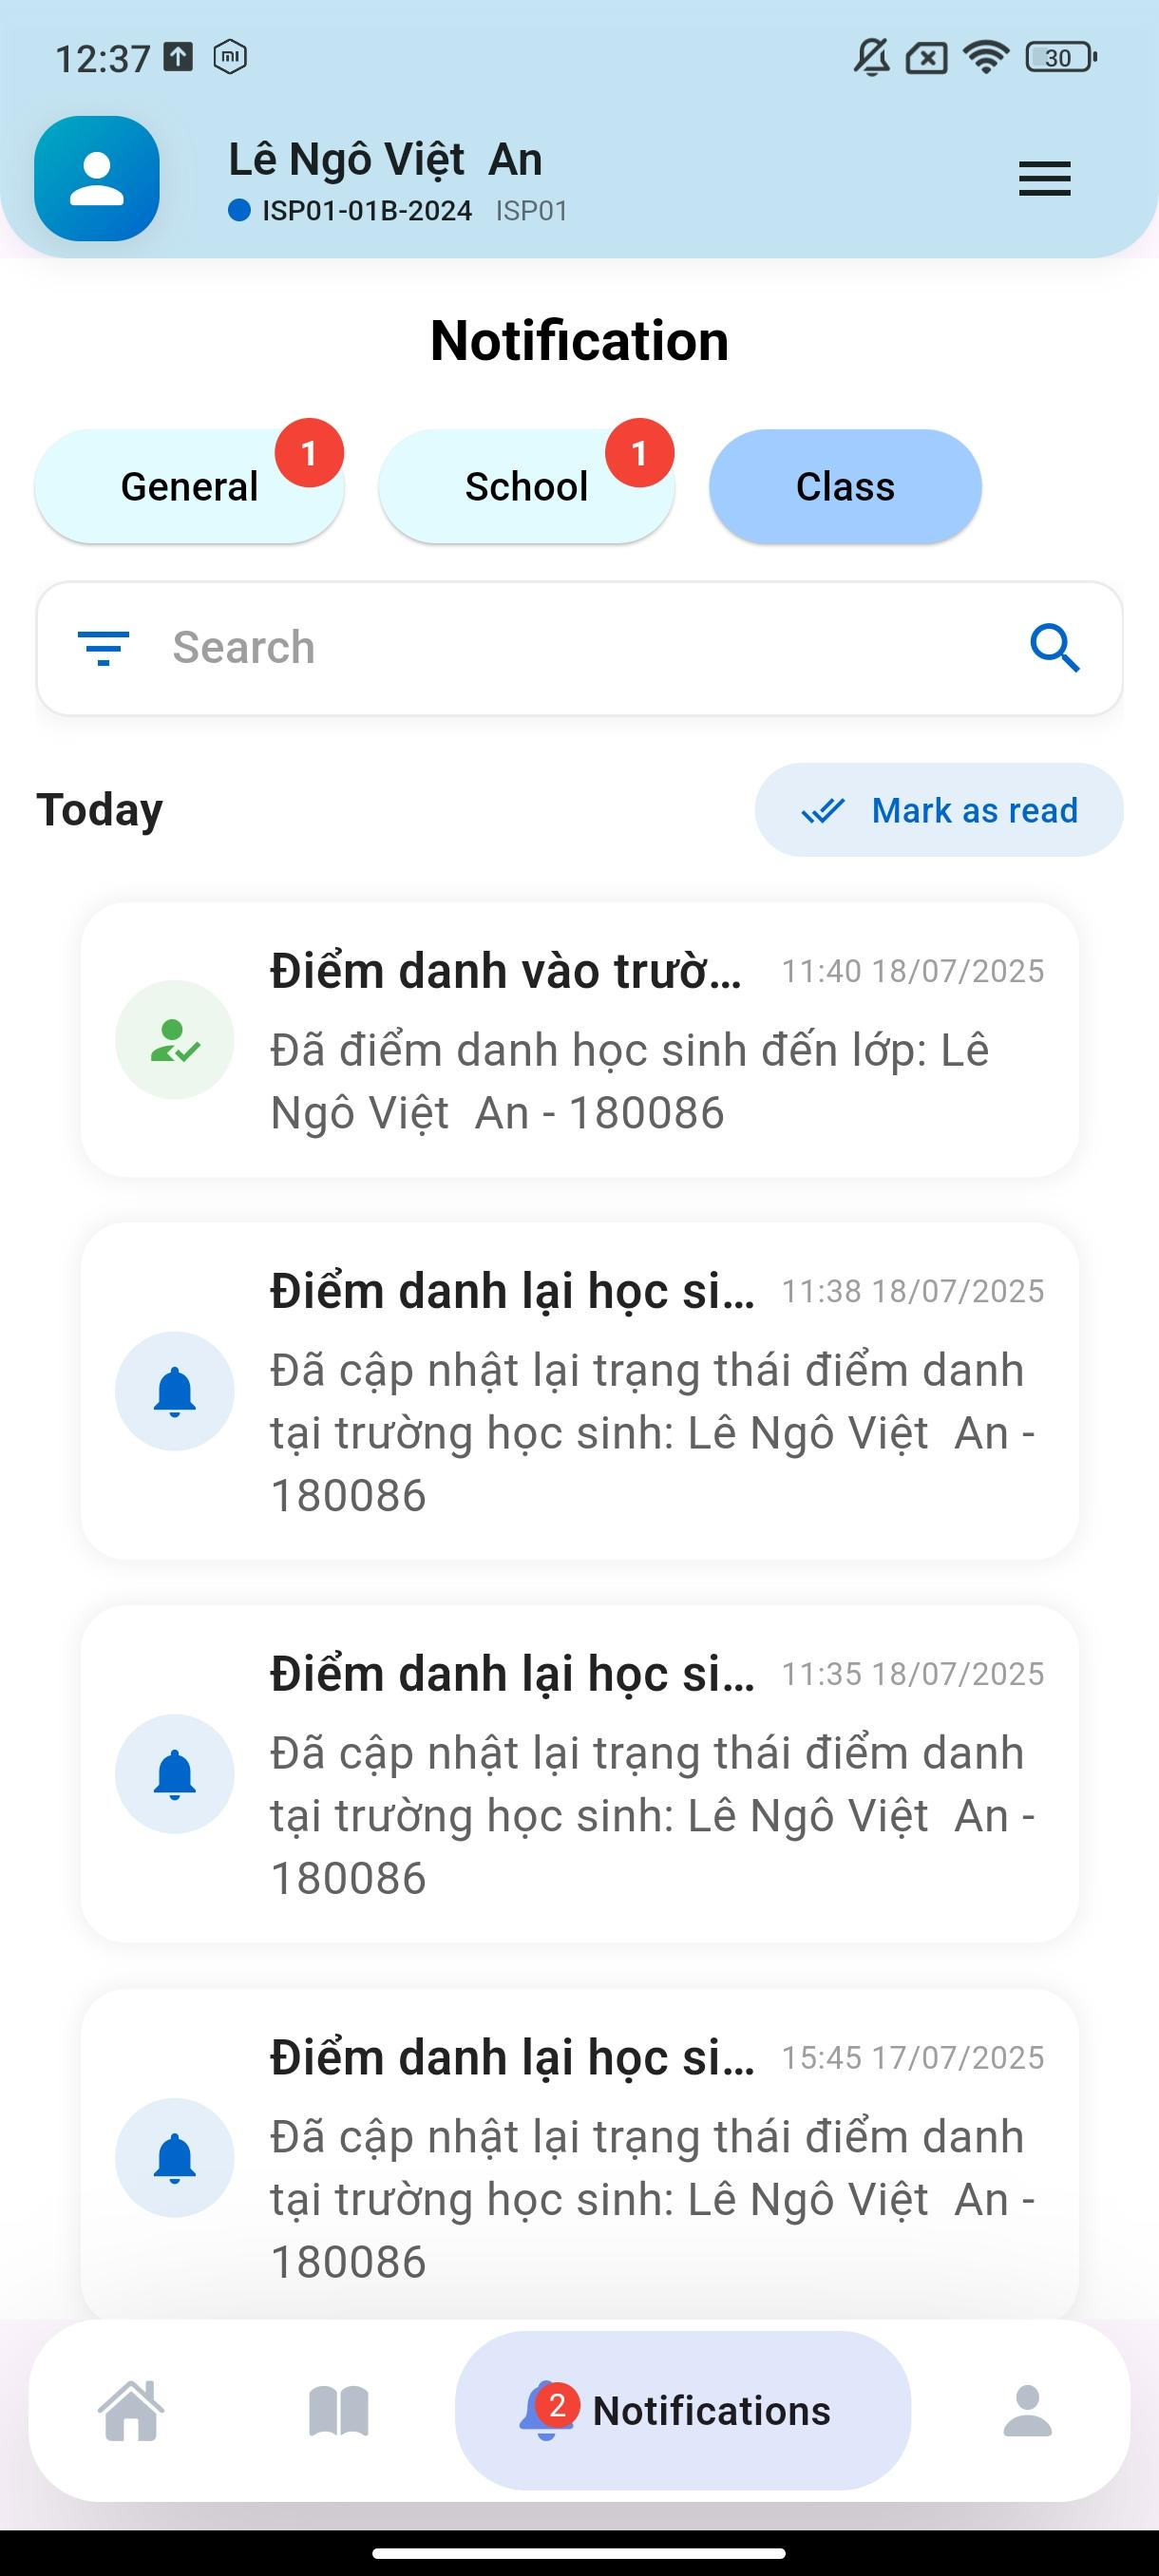
\includegraphics[width=0.6\textwidth]{images/notification_parent_view.png}
        \caption{Notification - Parent Create View}
        \label{subfig:notification_parent_view}
    \end{subfigure}
    \caption{Notification mobile app}
    \label{fig:notification_mobile_app}
    \end{figure}
    %-----------------
    \end{itemize}
\vspace{0.1cm}
\begin{minipage}{\textwidth}
    \setlength{\parindent}{2em}
   Additionally, I have \textbf{implemented and updated some key features} for the system such as:
\end{minipage}
\begin{itemize}[itemsep=-0.05cm, topsep=0.2cm]
    \item \textbf{Import/Export employee and student data}
    \item \textbf{Registering bus stop} (for mobile app)
    \item \textbf{Real-time Bus tracking} (for back-end part not the UI part)
\end{itemize}
\begin{minipage}{\textwidth}
    \setlength{\parindent}{2em}The modules and features I implemented have \textbf{passed almost all business test cases} and have been published for client verification. Additionally, I have \textbf{improved the system's performance} when handling large volumes of data, reducing the load time from minutes to just 3 seconds by \textbf{implementing pagination and multithreading}. Furthermore, the team and I have \textbf{collaborated to successfully publish the mobile application to the App Store and Google Play (CH Play)}, expanding accessibility for end users.
\end{minipage}
\begin{figure}[H]
    \centering
    
\includegraphics[width=0.35\textwidth]{images/ios_pathway.png}
    \caption{Mobile app on iOS}
    \label{subfig:ios_app}
\end{figure}
\begin{figure}[H]
    \centering
    
\includegraphics[width=0.6\textwidth]{images/android_pathway.png}
    \vspace{-1em}
    \caption{Mobile app on Android}
        \label{subfig:android_app}
\end{figure}


  % 5.2 Results
  % \subsection{Contributions}
  % \begin{minipage}{\textwidth}
    \setlength{\parindent}{2em}In this project, we focus on developing the mobile application of the system, enhancing the web application with new features, and maintaining the system and bug fixes. Specifically, we have implemented the following modules:
\end{minipage}\\
\begin{itemize}[itemsep=-0.05cm, topsep=0.1cm]
    \item \textbf{Leave Request Management} (for mobile)
    \item \textbf{Bus Management}
    \item \textbf{Newsfeed Management}
    \item \textbf{Assessments Management}
    \item \textbf{Health Management}
    \item \textbf{Notification Management}
\end{itemize}
\vspace{0.1cm}
\begin{minipage}{\textwidth}
    \setlength{\parindent}{2em}
   Additionally, we have implemented key features for the system such as:
\end{minipage}
\begin{itemize}[itemsep=-0.05cm, topsep=0.2cm]
    \item \textbf{Import/Export employee data}
    \item \textbf{Student attendance marking}
    \item \textbf{Student attendance reporting}
    \item \textbf{Bus tracking}
\end{itemize}
\vspace{0.2cm}
\begin{minipage}{\textwidth}
    \setlength{\parindent}{2em}The modules and features we implemented have \textbf{passed almost all business test cases} and have been published for client verification. Additionally, we have \textbf{improved the system's performance} when handling large volumes of data, reducing the load time from minutes to just 3 seconds by \textbf{implementing pagination and multithreading}. Furthermore, we \textbf{collaborated to successfully publish the mobile application to the App Store and Google Play (CH Play)}, expanding accessibility for end users.
\end{minipage}

  % 5.2 Discussions
  \subsection{Discussions}
  \begin{minipage}{\textwidth}
    \setlength{\parindent}{2em}
    Despite successfully implementing most of the modules and features assigned to me, a few challenges remain:
\end{minipage}\\
\vspace{-0.4cm}
\begin{itemize}[itemsep=-0.05cm]
    \item \textbf{Low performance}: Some features under my responsibility still suffer from performance issues, causing slow response times and negatively affecting the user experience.
    \item \textbf{Incomplete functionality}: The real-time bus tracking feature has been developed on the back end, but the user interface still needs to be implemented.
    \item \textbf{UI/UX Inconsistencies}: Some screens in the mobile app still lack design consistency, which may confuse users or reduce usability.
    \item \textbf{Limited Testing Coverage}: Due to time constraints, some modules were tested only under ideal conditions, which may lead to bugs in edge cases or on lower-end devices.
\end{itemize}

% \vspace{-0.2cm}
% \setlength{\parindent}{2em}The server performance issues primarily occur during high-traffic periods, such as morning attendance check-ins when hundreds of employees and students access the system simultaneously. These response delays, while not system-critical, can cause temporary inconvenience for users and may affect the efficiency of daily operations. We are actively monitoring server performance metrics and implementing optimization strategies to solve these bottlenecks.

% \vspace{0.1cm}
% \setlength{\parindent}{2em}Regarding incomplete features, the current production version represents a solid foundation with core HR and attendance management capabilities fully operational. However, several advanced modules outlined in the desired features remain in various stages of development.

% These pending features may include enhanced reporting dashboards, advanced analytics capabilities, integration modules for third-party educational software, or specialized functionalities requested by the client schools during the implementation process.

% \setlength{\parindent}{2em}The ongoing challenges highlight the iterative nature of enterprise software deployment, where continuous improvement and feature enhancement are essential for long-term success. The team's transparent acknowledgment of these issues demonstrates a commitment to quality and user satisfaction rather than rushing incomplete features to production.

% VII. CONCLUSION AND FUTURE SCOPE
\newpage
\section{ CONCLUSIONS AND FUTURE WORK}\label{sec:conclusion_and_future_scope}
\indent

  This section summarizes the key achievements and and outlines our strategic plans for future development.
  % 6.1 Results
  \subsection{Conclusions}
  \begin{minipage}{\textwidth}
    \setlength{\parindent}{2em}
    In conclusion, most of the objectives have been achieved. The majority of the modules and features assigned to me have been successfully developed and passed the required business test cases, demonstrating their stability and readiness for use. The backend APIs, built using Spring Boot, are efficient and well-structured, while the database design is secure, reliable, and consistent—effectively supporting the implemented features.

    The mobile application has been successfully published on both the Google Play Store and App Store. However, it is currently in the testing phase rather than in full production as initially expected. Once officially released, it is projected to serve around 5,000 students.

    Despite these achievements, there are still a few challenges to address, including low performance in some features, incomplete functionality in certain modules, and UI/UX inconsistencies.
\end{minipage}\\

% \setlength{\parindent}{2em}While the system faces ongoing challenges with server performance optimization and feature completion, these issues are characteristic of any ambitious software deployment and reflect the platform's continuous evolution rather than fundamental flaws. The transparent acknowledgment of these limitations, coupled with active development efforts to address them, demonstrates a mature approach to software lifecycle management and user satisfaction.

% \setlength{\parindent}{2em}The success at Inspire School and Pathway School serves as a compelling proof of concept for GMES School's potential to transform educational administration across Vietnam and beyond. As server performance improves and remaining features are implemented, the platform is well-positioned to expand its footprint in the educational sector. The combination of proven web-based functionality and the forthcoming mobile application creates a comprehensive solution that addresses the complex needs of modern educational institutions while providing the scalability necessary for future growth.

% \setlength{\parindent}{2em}The success at Inspire School and Pathway School serves as a compelling proof of concept for the GMES School system's potential to transform educational administration across Vietnam and beyond. The combination of proven web-based functionality and the forthcoming mobile application creates a comprehensive solution that addresses the complex needs of modern educational institutions while providing the scalability necessary for future growth.

% \setlength{\parindent}{2em}Ultimately, GMES School exemplifies how thoughtful technology design, iterative development, and user-focused implementation can create meaningful change in educational management, setting the stage for broader adoption and continued innovation in the sector.

  % 6.2 Discussions
  \subsection{Future Work}
  \begin{minipage}{\textwidth}
    \setlength{\parindent}{2em}
    To improve the system, several key areas for future development have been identified:
\end{minipage}\\
\vspace{-0.5cm}
\begin{itemize}[itemsep=-0.05cm]
    \item \textbf{Launch the mobile application}: The main priority is to release the mobile application to the production environment.
    \item \textbf{Boost performance}:Improve overall system performance by implementing load balancing and optimizing database connections to ensure reliable access for all users, even during peak usage across school institutions.
    \item \textbf{Add new features}: Continuously improve the system by completing existing features and adding new ones that meet the evolving needs of the school.
\end{itemize}

\newpage
\phantomsection
\addcontentsline{toc}{section}{REFERENCES}
\section*{REFERENCES}
\renewcommand{\refname}{} % This hides the default "References" title
% Patch the bibliography to remove the default horizontal rule
\makeatletter
\patchcmd{\thebibliography}
  {\section*{\refname}}  % This is the part inserting the heading and line
  {}                     % Replace it with nothing
  {}{}
\makeatother
 
\begin{thebibliography}{9}
\bibitem{vietname_education_2024_2025}
Minh Giảng. Toan canh giao duc viet nam 2024-2025. \textsc{url}: \url{https://tuoitre.vn/toan-canh-giao-duc-viet-nam-nam-hoc-2024-2025-2024090510153954.htm}.
\bibitem{what_is_sencha}
What is Sencha Ext JS? \textsc{url}: \url{https://pangea.app/glossary/sencha-ext-js}.
\bibitem{sencha_doc}
Sencha documentation \textsc{url}: \url{https://docs.sencha.com/extjs/7.9.0/}.
\bibitem{mvc_design_pattern}
Saket Kumar. MVC Design Pattern \textsc{url}: \url{https://www.geeksforgeeks.org/system-design/mvc-design-pattern/}.
\bibitem{flutter_doc}
Flutter documentation \textsc{url}: \url{https://docs.flutter.dev/}.
\bibitem{what_is_jvsb}
IBM. What is Java Spring Boot? \textsc{url}: \url{https://www.ibm.com/think/topics/java-spring-boot}.
\bibitem{what_are_microservices_g4g}
Tapan Rawat. What are Microservices? \textsc{url}: \url{https://www.geeksforgeeks.org/system-design/microservices/}.
\bibitem{what_is_microservices_architecture}
What is Microservices Architecture? \textsc{url}: \url{https://www.geeksforgeeks.org/system-design/microservices/}.
\bibitem{what_is_orm}
Ihechikara Abba. What is an ORM \- The Meaning of Object Relational Mapping Database Tools \textsc{url}: \url{https://www.freecodecamp.org/news/what-is-an-orm-the-meaning-of-object-relational-mapping-database-tools/}.
\bibitem{what_is_orm_baeldung}
Guilherme Chehab. What Is an ORM? How Does It Work? How Should We Use One? \textsc{url}: \url{https://www.baeldung.com/cs/object-relational-mapping}.
\bibitem{web_socket_explained}
Alex Diaconu. WebSockets explained: What they are and how they work \textsc{url}: \url{https://ably.com/topic/websockets}.
\bibitem{using_websocket_implement_with_stomp}
Tomasz Dabrowski. Using Spring Boot for WebSocket Implementation with STOMP \textsc{url}: \url{https://www.toptal.com/java/stomp-spring-boot-websocket}.
\bibitem{web_socket_with_spring}
Aliaksandr Liakh. WebSockets With Spring, Part 3: STOMP Over WebSocket \textsc{url}: \url{https://medium.com/swlh/websockets-with-spring-part-3-stomp-over-websocket-3dab4a21f397}.
\end{thebibliography}

% \newpage
% \phantomsection
% \addcontentsline{toc}{section}{APPENDICES}
% \section*{APPENDICES}
% \input{appendicies.tex}

\end{document}